\documentclass[a4paper]{book}

\setcounter{tocdepth}{0}
\usepackage{graphicx}
\usepackage[backend=biber,defernumbers=true]{biblatex}
%\defbibheading{chapbib}{%
%  \section{Publications}
%  \markboth{Publications}{Publications}
%}
\usepackage{hyperref}
% Chapter-local namespace for cross referencing
\newcommand{\localref}[1]{\ref{{\thechapter}_#1}}
\newcommand{\locallabel}[1]{\label{{\thechapter}_#1}}
%\usepackage{layout}
%\usepackage{showframe}
\usepackage[a4paper,top=1in,bottom=1in,left=1.25in,right=1in, marginparwidth=0in]{geometry}
\usepackage{multirow}
\usepackage{comment}

%%% for Japanese
\usepackage{CJKutf8}
\newcommand*{\Ja}[1]{%
  \begin{CJK}{UTF8}{ipxm}#1\end{CJK}}
%%%


\title{ACIS Annual Report FY2015}

\begin{document}

%\layout

\date{}

\maketitle
\tableofcontents

\chapter*{Preface}

\addcontentsline{toc}{chapter}{Preface}
\chapter*{Mission and Overview}

\addcontentsline{toc}{chapter}{Mission and Overview}
\chapter*{Organization}

\begin{figure}[h]
\centering
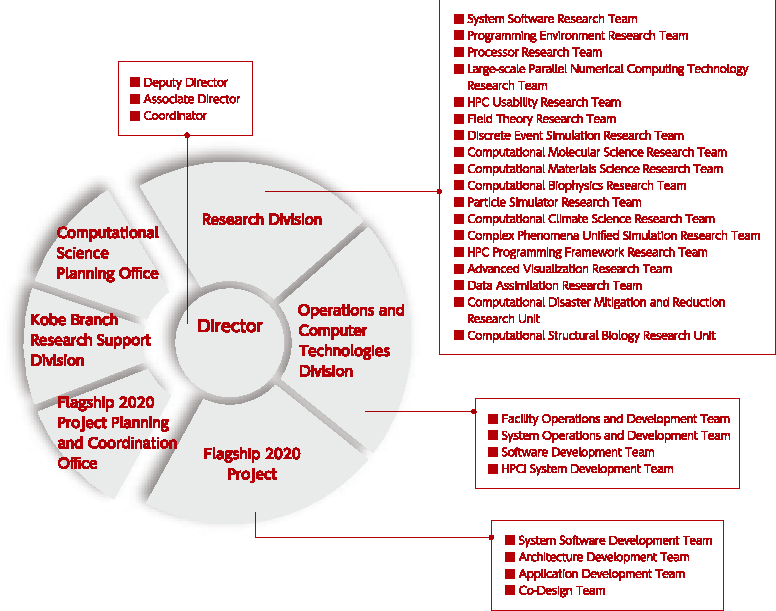
\includegraphics[width=\textwidth,keepaspectratio]{organization/organization-portrait.pdf}
\end{figure}

\addcontentsline{toc}{chapter}{Organization}

\begin{refsection}[sample_division/sample_group/group.bib]
\nocite{*}
\chapter{Sample Group}

\section{Members}

\begin{itemize}
  \item[] Ichiro Kobe (Team Leader)
  \item[] Jiro Kobe (Senior Scientist)
  \item[] Saburo Kobe (Research Scientist)
\end{itemize}

\section{Research Activities}

Text for research activities.

\section{Research Results and Achievements}

Text for research Results and achievements. Journal-artcile~\cite{sample-journal}.
Conference-paper~\cite{sample-conference}.
Invited-talk~\cite{sample-invited}.

For cross referencing, use \verb|\locallabel| and \verb|\localref| to avoid conflicting names defined by other groups. For example, a figure can be referenced as Figure~\localref{fig:sample-label1}.

\begin{figure}
\centering
  
\includegraphics[width=0.5\textwidth,keepaspectratio,natwidth=193,natheight=40]
  {sample_division/sample_group/test1.png}
  \caption{Caption for a sample figure}
  \locallabel{fig:sample-label1}
\end{figure}

\section{Schedule and Future Plan}

Text for schedule and future plan.

%%% DO NOT EDIT BELOW

\section{Publications}

%\printbibliography[keyword=journal, heading=subbibliography, title={Journal Articles}, prefixnumbers={1-}, resetnumbers=true]
%\printbibliography[keyword=proceedings, heading=subbibliography, title={Conference Papers}, prefixnumbers={2-}, resetnumbers=true]
%\printbibliography[keyword=invited, heading=subbibliography, title={Invited Talks}, prefixnumbers={3-}, resetnumbers=true]
%\printbibliography[keyword=poster, heading=subbibliography, title={Posters and Presentations}, prefixnumbers={4-}, resetnumbers=true]
%\printbibliography[keyword=deliverable, heading=subbibliography, title={Patents and Deliverables}, prefixnumbers={5-}, resetnumbers=true]

\printbibliography[keyword=journal, heading=subbibliography, title={Journal Articles}, resetnumbers=true]
\printbibliography[keyword=proceedings, heading=subbibliography, title={Conference Papers}]
\printbibliography[keyword=invited, heading=subbibliography, title={Invited Talks}]
\printbibliography[keyword=poster, heading=subbibliography, title={Posters and Presentations}]
\printbibliography[keyword=deliverable, heading=subbibliography, title={Patents and Deliverables}]

\end{refsection}


\part{Research Division}

\chapter*{}

This part presents the research activity of the Research Division of RIKEN Advanced Institute for Computational Science (AICS) for the period of 1 April 2015 to 31 March 2016.

This is the sixth year for AICS since its foundation in 2010.  The Research Division continued to operate with 16 teams and 3 units as established in 2012.  As of 1 April 2014, the number of researchers in the Division was 126 in total.

The research activity in this fiscal year resulted in ??? journal papers, ??? conference reports, ??? invited talks, ??? posters and presentations, ??? patents and deliverables.

Memorable awards bestowed upon AICS researchers included No. 1 ranking on Graph500 in June and November 2015, back from No. 2 in November 2014.  Combined with the No. 4 position on Top500 Ranking and No. 2 on HPCG ranking maintained through 2015, they continued to illustrate the well-balanced and versatile performance of the K computer in its 4th year of operation.

Many research-related events took place in this fiscal year.  The 6th AICS International Symposium, which became an annual event at Kobe, was held on 22 – 23 February 2016 under the title “Plans and future for international collaborations on extreme scale computing”.  AICS also hosted “Lattice 2015 – the 33rd International Symposium on Lattice Field Theory” on 14 – 18 July, 2015, a major conference in the field of computational particle physics.

We hope that this volume conveys the excitement of research and development at the forefront of computational and computer science being conducted at Research Division of RIKEN AICS to readers.

\vspace{1cm}

\noindent
July 2016

\begin{flushright}
Akira Ukawa\\
Research Division Director\\
and Deputy Director\\
RIKEN AICS
\end{flushright}

\begin{refsection}[research/ishikawa/group.bib]
\nocite{*}
\chapter{System Software Research Team}
%=============================================================================
\section{Members}
%=============================================================================

\begin{itemize}
  \item[] Yutaka Ishikawa (Team Leader)
  \item[] Atsushi Hori (Senior Scientist)
  \item[] Yuichi Tsujita (Research Scientist)
  \item[] Kazumi Yoshinaga (Postdoctoral Researcher)
  \item[] Akio Shimada (Research Associate)
  \item[] Masayuki Hatanaka (Research Associate)
  \item[] Norio Yamaguchi (Research Associate)
  \item[] Toyohisa Kameyama (Technical Staff)
\end{itemize}

%=============================================================================
\section{Research Activities}
%=============================================================================
The system software team focuses on the research and development of an
advanced system software stack not only for the "K" computer but also
for towards exascale computing.  There are several issues in carrying
out future computing. Two research categories are taken into account:
i) scalable high performance libraries/middleware, such as file I/O
and low-latency communication, and ii) a scalable cache-aware, and
fault-aware operating system for next-generation supercomputers based
on many core architectures.

%==============================================================================
\section{Research Results and Achievements}
%==============================================================================

%------------------------------------------------------------------------------
\subsection{PRDMA (Persistent Remote Direct Memory Access)}
%------------------------------------------------------------------------------
%The goal of this research is to design and evaluate an efficient MPI
%implementation for neighborhood communication by taking advantage of
%the Tofu interconnect, which has multiple RDMA (Remote Direct Memory
%Access) engines and network links per MPI process. The neighborhood
%communication pattern is commonly used in the ghost (or halo) cell
%exchanges.

The PRDMA (Persistent RDMA)\cite{dist-prdma} is an enhancement of MPI persistent
communication primitives to reduce the communication latency and to
improve the overlap between computation and communication over an
RDMA-enabled interconnect. The RDMA-base transfers can progress the
non-blocking communication without CPU intervention, and reduce extra
copy overheads and memory consumption for data transfers due to the
Zero-Copy feature. The MPI persistent communication is defined in MPI
standard since MPI version 1.1 specification. For example, when
calling with the same communication parameters from an iterative
stencil loop, the MPI persistent communication can avoid the redundant
setup cost on every call, including the RDMA buffer address
exchanges. Also, the initial costs to schedule the communication
requests are amortized over a number of stencil iterations.

We implemented the prototype of the PRDMA protocol over the Open MPI
provided on the K computer in FY2012. In FY2013, We improved the
performance in the ghost cell exchange pattern, such as derived
datatype handling and special handling upon non-periodic boundary
condition.
Furthermore, we applied the PRDMA to an optimized prototype
implementation of MPI-3 Neighborhood Collectives, as known as
MPI\_Neighbor\_alltoallw, over MPICH on the K computer in FY2014.

In FY2015, we improved the quality of the MPICH on K computer, and
made it available for public use on the K computer. In addition, we
have been implementing the prototype of the PRDMA-based MPI-RMA
implementation on the Tofu2 interconnect of FX100 to compare with the
MPI-3 neighborhood collectives. The MPI-RMA passive synchronization
such as MPI\_Win\_lock / unlock does not require the involvement of
target process. To implement a truly passive locking on the FX100, we
designed a distributed lock queue using RDMA Atomic operations of
Tofu2 interconnect. In Figure \localref{fig:prdma}, the vertical axis shows the elapsed
time in second for 1000 calls of MPI\_Win\_lock and MPI\_Win\_unlock with
MPI\_LOCK\_SHARED, and the horizontal axis shows the number of MPI
processes which acquires the same lock. The FX10 indicates the result
of the Open MPI based generic implementation without RDMA Atomics. The
FX100 indicates the result of the MCS-based Readers-Writer lock
(Readers Preference) implementation using Tofu2 RDMA Atomics. The
FX100 achieves 130 [us] at 256 processes (114 [s] in FX10).

\begin{figure}
\begin{center}
 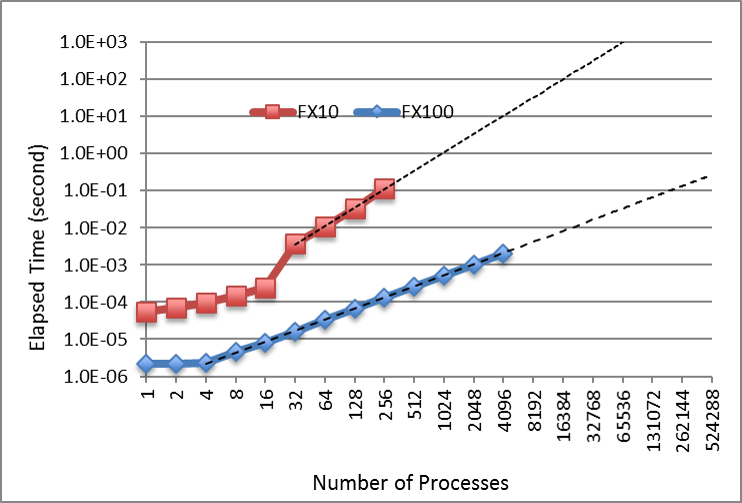
\includegraphics[width=0.7\textwidth,natwidth=557,natheight=377]{mpich-winlock.png}
\end{center}
  \caption{Benchmark Result of MPI\_Win\_lock / unlock with empty critical section}
  \locallabel{fig:prdma}
\end{figure}

%------------------------------------------------------------------------------
\subsection{OFI/LLC and RMPI}
%------------------------------------------------------------------------------
\begin{figure}
\begin{center}
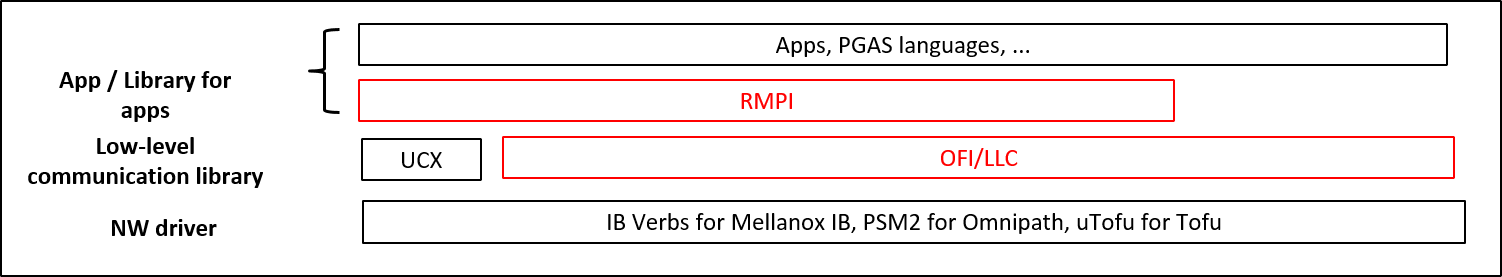
\includegraphics[width=0.8\textwidth,natwidth=1127,natheight=208]{mpich1.png}
\end{center}
 \caption{Relationships between applications, communication libraries and network driver}
 \locallabel{fig:mpich1}
\end{figure}

Two communication libraries have been developed. The first one is
called Low-Level Communication Library, which will adopt Open Fabric
Interface (OFI) and is called OFI/LLC. The second one is called
RIKEN-MPI (RMPI) which is based on MPICH. The relationships between
applications, RMPI, OFI/LLC and network drivers are explained by using
Figure \localref{fig:mpich1}. A network driver provides communication
functions to OFI/LLC. OFI/LLC provides communication functions to both
parallel language runtimes (e.g. MPI library) and applications
(e.g. visualization) via a low-level interface. RMPI provides
communication functions to applications via a high-level interface.

\begin{figure}
\begin{center}
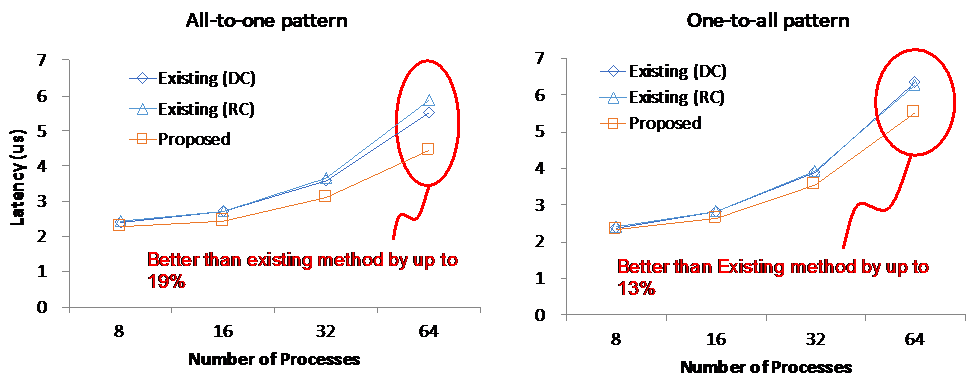
\includegraphics[scale=0.8,natwidth=703,natheight=276]{mpich2.png}
\end{center}
 \caption{Communication latency in all-to-one and one-to-all communication patterns}
 \locallabel{fig:mpich2}
\end{figure}

Two optimizations are performed in FY2015\cite{takagi2015}.  The first optimization
finds the proper numbers for different kinds of hardware contexts at
run-time.  The purpose is to maximize the performance while limiting
its memory consumption to the amount at which it is possible to run
parallel applications with millions of compute nodes.

The conventional network hardware provides a communication model in
which the memory-area for communication information for an end-point
pair (called context) is never released at run-time. The next
generation network hardware adds a new communication model in which
the memory-area can be allocated and released at run-time to save
memory. However, you lose performance just to make all end-point pairs
use the new model because it has a certain amount of performance
overhead when allocating. Therefore, it is needed to find how many
end-point pairs should use the conventional model and how many the new
model. We propose a method to find the proper combination of the
number-pair at run-time. This is done by calculating the benefits of
different combinations of the number-pair at run-time by using the
communication statistics and an analytic model. It was implemented
in OFI/LLC and evaluated using two micro-benchmarks performing
all-to-one and one-to-all types of communications. The latency is
reduced by up to 19\% and 13\%, respectively, as shown in Figure
\localref{fig:mpich2}.

\begin{table}
 \caption{Memory consumption per compute node of MPICH and LLC}
         \locallabel{tab:mpich}
%% 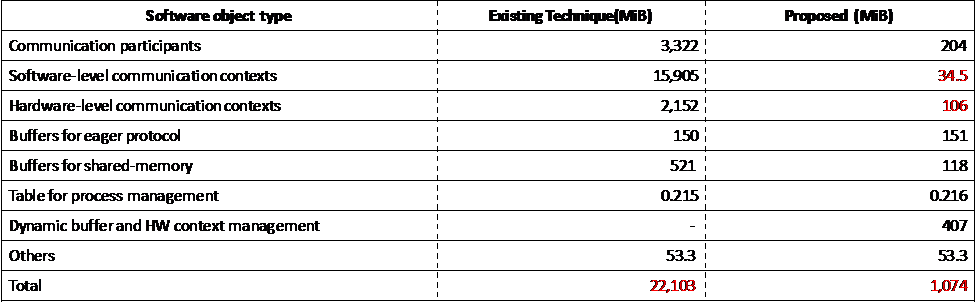
\includegraphics[natwidth=702,natheight=220]{mpich3.png}
\begin{center}
\begin{tabular}{l|r|r} \hline
Software object type &           Existing Technique (MiB) &      Proposed (MiB) \\ \hline
Communication participants &            3,322   & 204 \\
Software-level communication contexts & 15,905  & 34.5 \\
Hardware-level communication contexts & 2,152   & 106 \\
Buffers for eager protocol &            150     & 151 \\
Buffers for shared-memory &             521     & 118 \\
Table for process management &          0.215   & 0.216 \\
Dynamic buffer and HW context management & -    & 407 \\
Others &                                53.3    & 53.3 \\
Total &                                 22,103  & 1,074 \\ \hline
\end{tabular}
\end{center}
\end{table}

The second optimization is for the both OFI/LLC and RMPI libraries. It
tries to keep only active software contexts in memory. The
purpose is to limit the per-node memory consumption with the same
target as the first optimization.

The conventional communication libraries prepare software contexts of
the number proportional to the number of MPI processes. The proposed
method only keeps a constant number of software contexts in memory by
releasing inactive contexts when necessary. The mechanism was
evaluated by using an analytic model of the memory consumption which
is created by analyzing source code of OFI/LLC and MPICH. Table
\localref{tab:mpich} shows the memory consumption with 4,194,304 MPI
processes on 1,048,576 compute nodes. The proposed method reduces the
memory consumption per compute node from 22~GiB to 1~GiB when compared
to the existing technique.

%------------------------------------------------------------------------------
\subsection{Scalable MPI-IO Using Affinity-Aware Aggregation}
%------------------------------------------------------------------------------
\begin{figure}
\begin{center}
 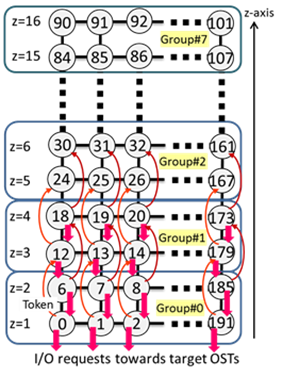
\includegraphics[width=0.5\textwidth,natwidth=204,natheight=271]{earth1.png}\\
(a) I/O throttling approach
\end{center}
\begin{center}
 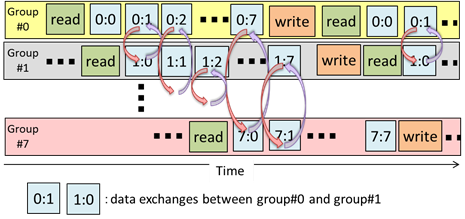
\includegraphics[width=0.7\textwidth,natwidth=335,natheight=158]{earth2.png}\\
(b) associated stepwise data exchanges
\end{center}
  \caption{Optimization Techniques in EARTH} \locallabel{fig:earth1}
\end{figure}

A commonly used MPI-IO library named ROMIO has the two-phase I/O
(TP-IO) scheme to improve collective I/O performance for
non-contiguous accesses. This research is addressing to optimize TP-IO
implementation for further I/O performance improvements than the
original one.
In the FY2015, we have proposed enhanced TP-IO approach named EARTH
(Effective Aggregation Rounds with THrottling) in the MPI library at
the K computer\cite{tsujita2015}. It has been arranged to have cooperative stepwise data
exchanges based on the optimized aggregator layout and I/O throttling
approach done in the FY2014. Its I/O throttling scheme and stepwise
data exchanges are illustrated in Figure \localref{fig:earth1}.

Figure \localref{fig:earth1}(a) illustrates I/O throttling approach of the
EARTH using token-relay. EARTH divided processes into groups which are
associated with target Object Storage Target (OST) of the FEFS file
system on the K computer. Then the EARTH throttles I/O request
generation of each process, where process that receives a token issues
I/O request. As a result, network and I/O request contention can be
minimized. Furthermore, stepwise data exchanges in Figure
\localref{fig:earth1}(b) improve data exchange times by splitting
all-to-all manner data exchanges into sub-groups which are associated
with I/O throttling. This stepwise data exchange scheme has two
advantages compared with the original all-to-all manner data
exchanges. One is minimization in waiting time to complete data
exchanges. Another is mitigation of network contention.

Performance evaluation was carried out using computing nodes ranged
from 192 to 3,072 nodes. I/O performance evaluation was done by using
the HPIO benchmark with non-contiguous access patterns on a local file
system of the FEFS on the K computer. The number of nodes was arranged
not to have any interference from other users' applications. In the K
computer case, we specified the number of nodes in a 3D manner node
allocation, where we chose the following five patterns; 2x3x32,
4x3x32, 8x3x32, 8x6x32, and 8x12x32. We deployed one MPI process per
one computing node, thus the number of MPI processes was the same with
that of used computing nodes. Figure \localref{fig:earth2} shows I/O
throughput values relative to the number of MPI processes.

\begin{figure}
\begin{center}
 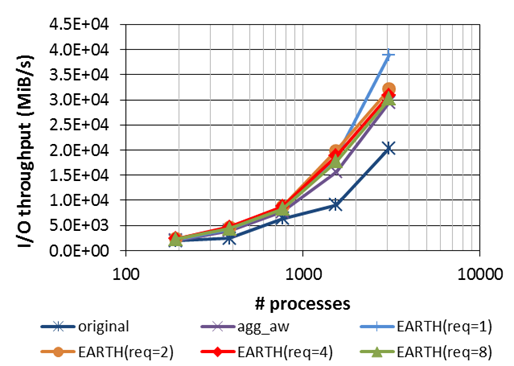
\includegraphics[natwidth=370,natheight=264]{earth3.png}
\end{center}
  \caption{I/O throughput of collective write}
  \locallabel{fig:earth2}
\end{figure}

In this evaluation, we examined the number of I/O requests for 1, 2,
4, and 8 in the I/O throttling scheme indicated by
{\it EARTH(req=1)}, {\it EARTH(req=2)}, {\it EARTH(req=4)},
and {\it EARTH(req=8)}, respectively
in addition to the original implementation indicated by {\it original}
and aggregator layout optimization only version ({\it agg\_aw}). The
EARTH optimization outperformed the original one and aggregator layout
optimization only version. From this evaluation, one I/O request case in
the EARTH optimization was the best when we had 3,072 processes. Our
future work is the way for tuning the number of I/O requests to gain
the best I/O performance.

%------------------------------------------------------------------------------
%\subsection{Partitioned Virtual Address Space}
\subsection{New Process / Thread Model}
%------------------------------------------------------------------------------
From FY2012, we have been developing a new process/thread model that
is suitable for the many-core architectures. The many-core
architectures are gathering attention towards the next generation
supercomputing. Many-core architectures have a large number of low
performance cores, and then the number of parallel processes within a
single node becomes larger on many-core environments. Therefore, the
performance of inter-process communication between the parallel
processes within the same node can be an important issue for parallel
applications.

Partitioned Virtual Address Space (PVAS) is a new execution model to
achieve high-performance inter-process communication on the many-core
environments. With PVAS, multiple processes run in the same virtual
address space as shown in Figure \localref{fig:pvas} to eliminate the
communication overhead due to the process boundaries that the current
modern OSes introduce for inter-process protection. In PVAS, the data
owned by the other process can be accessed by the normal load and
store machine instructions, just like the same way accessing the data
owned by itself. Thus, high-performance inter-process communication is
achieved.

We implemented the prototype of the PVAS execution model in the Linux
kernel in FY2012. We improved its quality and published it as open
source software in FY2013. To demonstrate the potential of PVAS, Open
MPI has been modified to utilize PVAS since then\cite{shimada2015}. Especially in
FY2015, proposed and developed PVAS was ported to McKernel.

\begin{figure}
\begin{center}
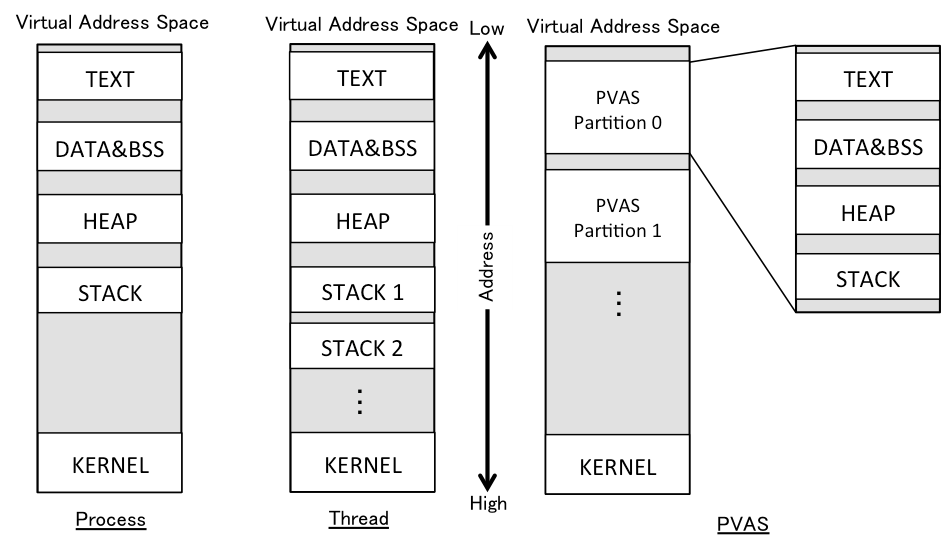
\includegraphics[width=0.7\textwidth, natwidth=678,natheight=391]{pvas.png}
\end{center}
 \caption{Partitioned Virtual Address Space}\locallabel{fig:pvas}
\end{figure}

It is already known that process oversubscription, which binds multiple parallel processes
to one CPU core, can hide the communication latency and reduce CPU
idle time. However, the lightweight OS kernels for Exascale systems
may no longer support OS task scheduling to reduce OS noise. Without
OS task scheduling, only one parallel process per CPU core is allowed
to run, and the process oversubscription is impossible. Even if the OS
task scheduling is supported, the overhead of the context switch
hinders the application performance and ruins the advantage of
process oversubscription. 

To tackle this issue, we proposed user-level process
(ULP) in FY2015. The user-level process is a process which can be scheduled in
the user-space. The ULP was implemented as an extension of PVAS. ULP
has the beneficial features of the user-level
thread. Meanwhile, it has its own program code and data like a
traditional process. By assigning a role of a parallel process to a
user-level process, high-performance process oversubscription can be
achieved without OS task scheduling. Moreover, the process
oversubscription utilizing ULP does not change the 
programming model of the parallel application.

The context switching times of conventional Linux process, Linux
thread and ULP over the number of execution entities are compared in
Figure \localref{fig:pvas-contextswitch}. Theoretically, there is no need
of calling any systemcall to switch user-level processes, however, the
privileged FS segment register is used to point Thread Local Storage
(TLS) must be switched at the time of context switch on the x86 CPU
architecture. As shown in Figure \localref{fig:pvas-contextswitch}, the
fastest one is ULP without switching the FS register, and send fastest
one is ULP with the FS switching. Anyway the context switching times
of conventional processes (KLP) and threads (KLP) are much higher than
those of ULPs.

\begin{figure}
\begin{center}
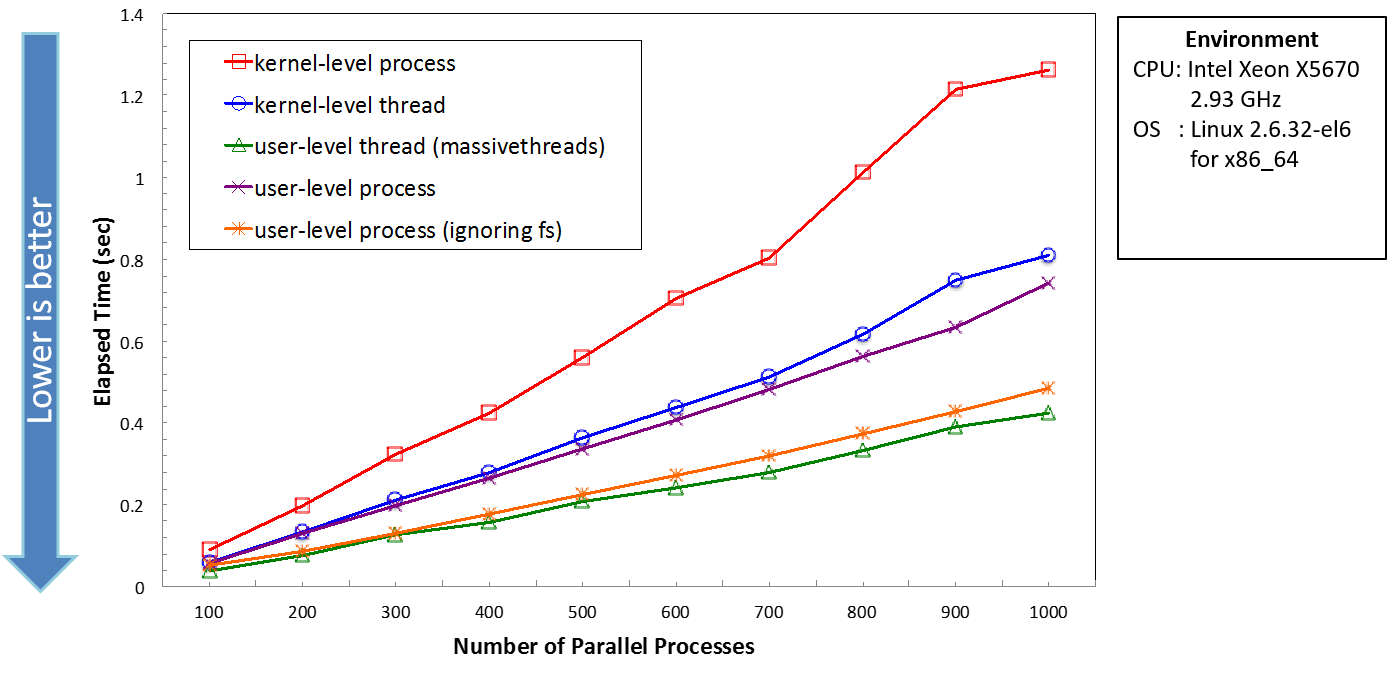
\includegraphics[width=0.8\textwidth,natwidth=1040,natheight=506] {pvas-contextswitch.png}
\end{center}
 \caption{Context Switching Time (KLP, KLT and ULP)}\locallabel{fig:pvas-contextswitch}
\end{figure}

%------------------------------------------------------------------------------
\subsection{Fault Resilience}
%------------------------------------------------------------------------------
With the increasing fault rate on high-end supercomputers, the topic
of fault tolerance has been gathering attention. To cope with this
situation, various fault-tolerance techniques are under investigation;
these include user-level, algorithm-based fault-tolerance techniques
and parallel execution environments that enable jobs to continue
following node failure. Even with these techniques, some programs,
such as stencil computation, having no dynamic load balancing function
may underperform after a failure recovery. Even when spare nodes are
present, they are not always substituted for failed nodes in an
effective way.

There are some questions of how spare nodes should be allocated, how
to substitute them for faulty nodes, and how much the communication
performance is affected by such a substitution. The third question
stems from the modification of the rank mapping by node substitutions,
which can incur additional message collisions. In a stencil
computation, rank mapping is done in a straightforward way on a
Cartesian network without incurring any message collisions. However,
once a substitution has occurred, the node-rank mapping may be
destroyed. Therefore, these questions must be answered in a way that
minimizes the degradation of communication performance.

\begin{figure}
\begin{center}
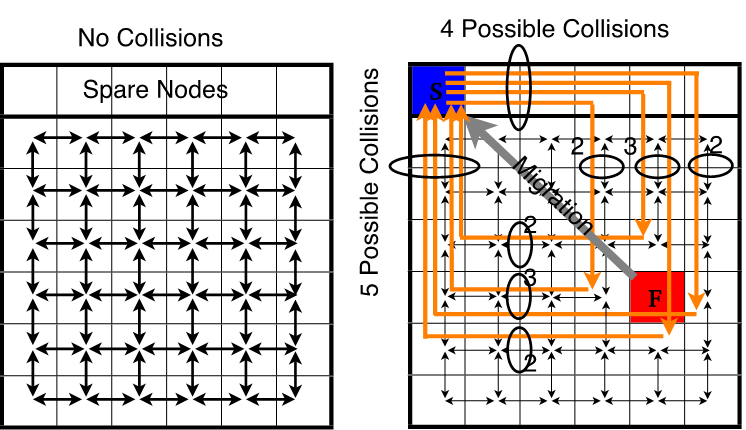
\includegraphics[width=0.7\textwidth,natwidth=373,natheight=215] {resilience1.png}
\end{center}
 \caption{Message collisions by substituting a failed node (5P-stencil)}\locallabel{fig:resilience1}
\end{figure}

Several spare-node allocation and node-substitution methods
had been proposed, compared and analyzed in terms of communication
performance(Figure \localref{fig:resilience1})\cite{hori2015}.

\begin{figure}
\begin{center}
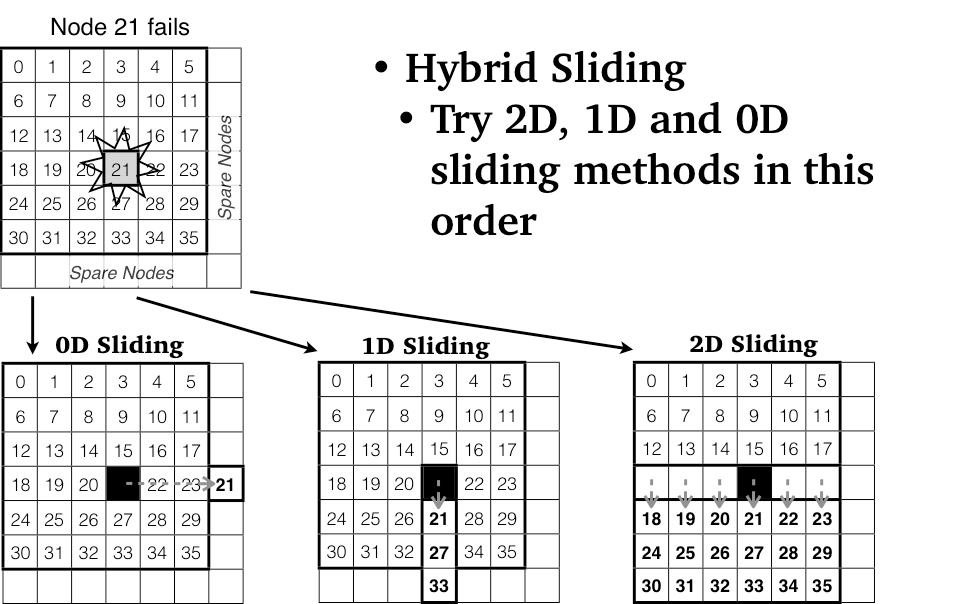
\includegraphics[width=0.7\textwidth,natwidth=958,natheight=604] {resilience2.png}
\end{center}
 \caption{Proposed Three Failed Node Substitution Methods}\locallabel{fig:resilience2}
\end{figure}

In FY2015, the proposed methods were evaluated using BlueGene Q (JUQUUEN at J\"ulich Supercomputing Center) and the K computer.
Figure \localref{fig:resilience2} shows the communication performance
degradation on the K computer\cite{yoshinaga2015}. The black lines represent the
simulation results with 3D mesh network having the same size with the
K computer evaluation (12x12x12) and the red lines represent the
evaluation results of the K computer. In all cases, the hybrid sliding
method is used. Left graph shows the cases with 7P stencil
communication pattern (4 MiB), upper right graph shows the cases with
the barrier collective communication, and the lower right graph shows
the allreduce collective communication (16 KiB). Figure
\localref{fig:resilience3} shows the communication performance on BG/Q with
the same way as in Figure cite{fig:resilience2}, unless otherwise
noted.

\begin{figure}
\begin{center}
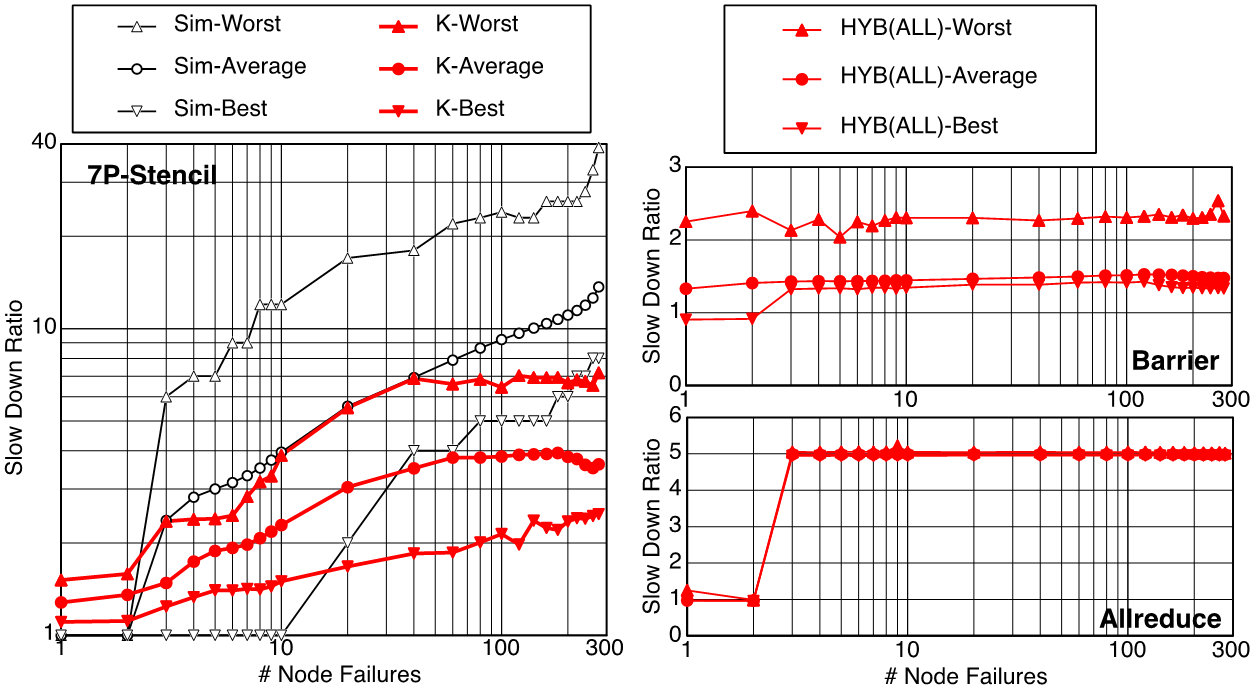
\includegraphics[width=0.8\textwidth,natwidth=628,natheight=347] {resilience3.png}
\end{center}
 \caption{Communication Performance Degradation by Using Spare Nodes 
the K computer (12x12x12)}\locallabel{fig:resilience3}
\end{figure}

\begin{figure}
\begin{center}
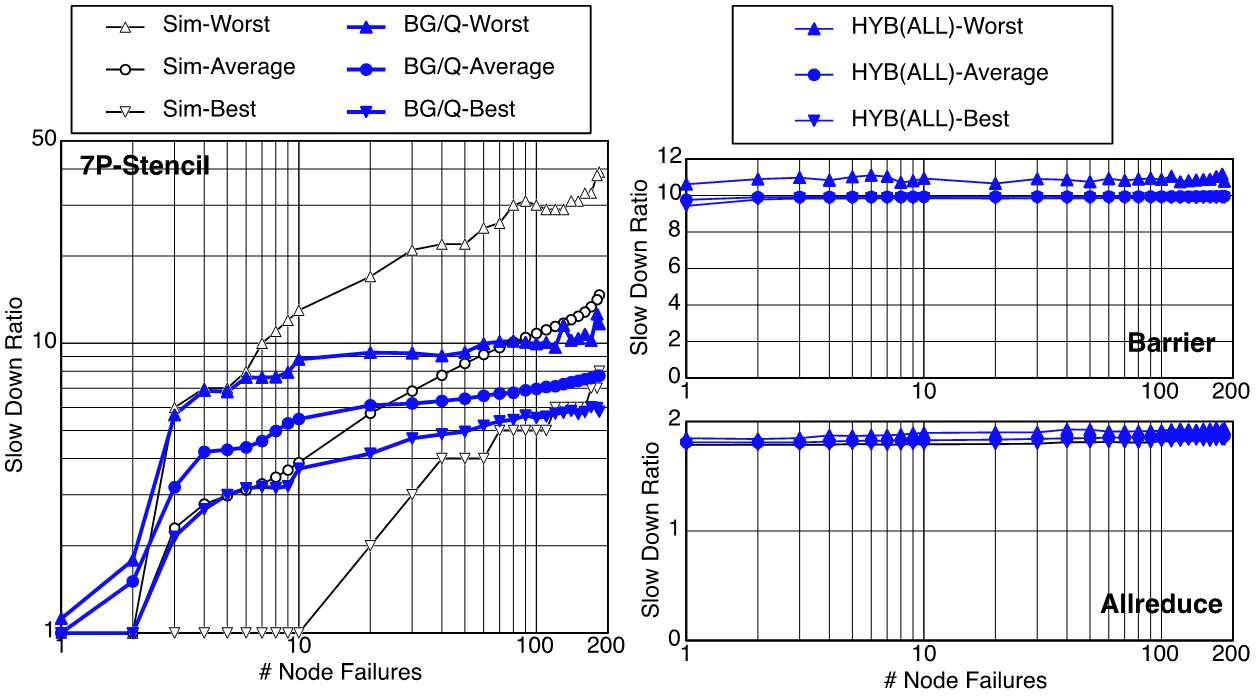
\includegraphics[width=0.8\textwidth,natwidth=904,natheight=499] {resilience4.png}
\end{center}
 \caption{Communication Performance Degradation by Using Spare Nodes 
the K computer (12x12x12)}\locallabel{fig:resilience4}
\end{figure}

As shown in Figures \localref{fig:resilience3} and
\localref{fig:resilience4}, the actual patterns of the stencil
communication performance degradation can vary in the K computer and
BG/Q. The collective communication performance degradation, however,
is relatively constant over the number of failed nodes.

%------------------------------------------------------------------------------
\subsection{Big data processing on the K computer}
%------------------------------------------------------------------------------
This research was conducted by collaboration between the Data
Acquisition team of RIKEN SPring-8 Center and the System Software
Research team of RIKEN AICS. The goal of this project is to establish
the path to discover the 3D structure of a molecule from a number of
XFEL (X-ray Free Electron Laser) snapshots. The K computer will be used to
analyze the huge data transmitted from RIKEN Harima where SACLA XFEL
facility is located.

In order to reduce quantum noise, each representative image must be
averaged out more than hundred images. In addition to this, the
sampled X-ray images must cover all possible orientations of the
molecule. The number of images, although it depends on desired
accuracy and the size of the molecule, can be one million in typical
cases. Thus, the massive power of the K computer is needed.

\begin{figure}
\begin{center}
 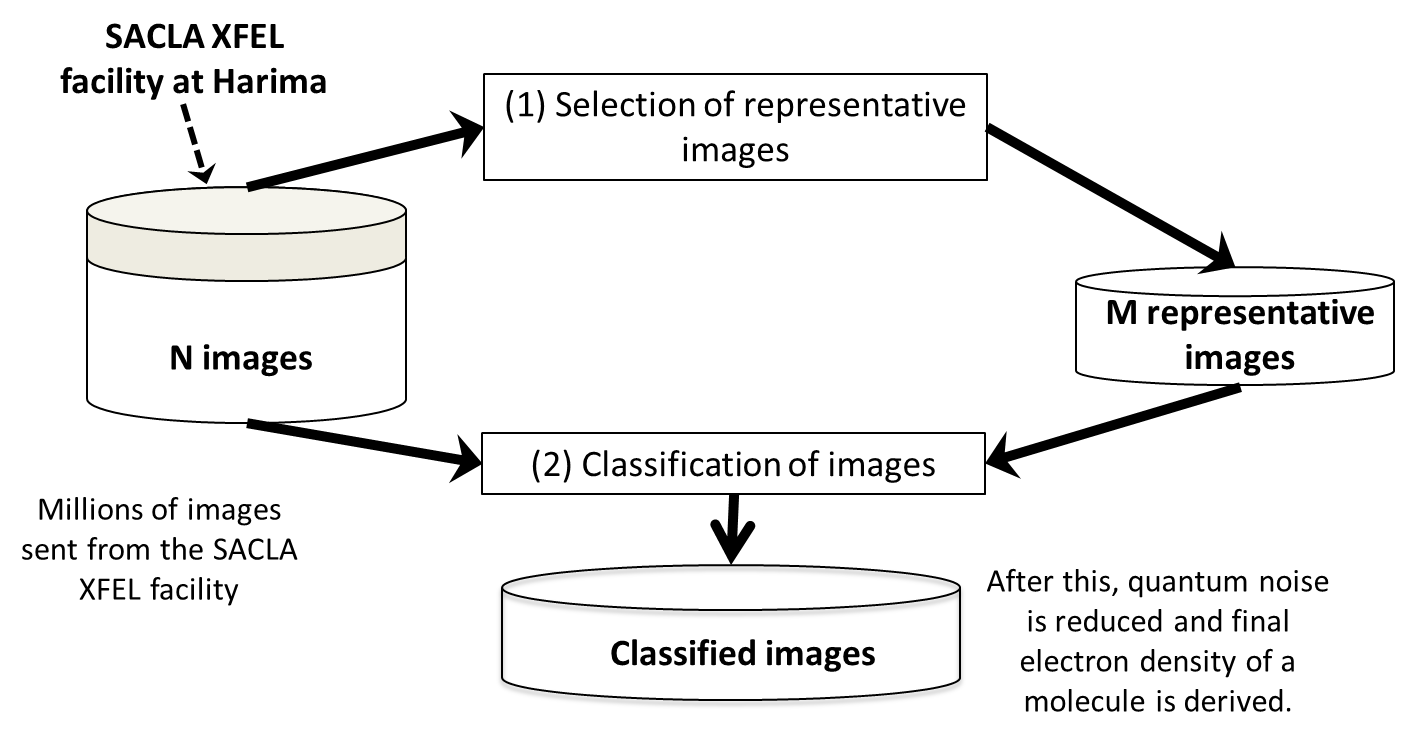
\includegraphics[width=0.7\textwidth,natwidth=1013,natheight=534] {carp1.png}
\end{center}
  \caption{Block diagram of the procedure running on the K computer}\locallabel{fig:carp1}
\end{figure}

We had developed a parallel software running on the K
computer to analyze images obtained by a light source, SACLA. The
developed software consists of two components as shown in \localref{fig:carp1}. The first phase is to select the representative images by a classic
clustering computation. Thus, all images must be compared with all
others. The second phase is to classify the rest of images into the
representative images. In this stage, we need to calculate for all
possible combinations of representative images and rest of the images.

\begin{figure}
\begin{center}
 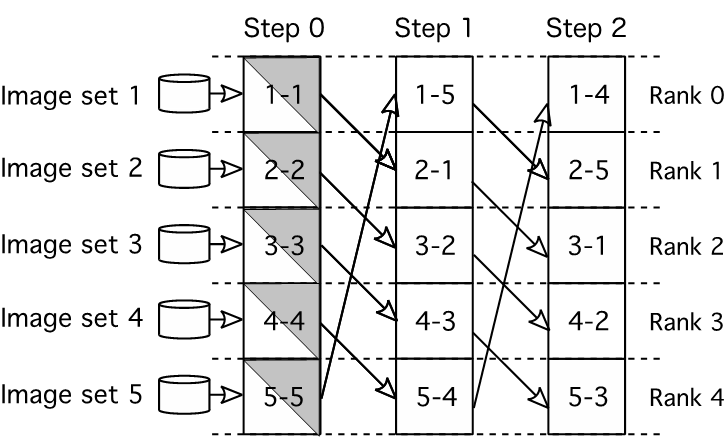
\includegraphics[width=0.7\textwidth,natwidth=523,natheight=316] {carp3.png}
\end{center}
  \caption{I/O minimization and load balancing}\locallabel{fig:carp3}
\end{figure}

After developing the first version of the program, 
we started to develop a new framework, named pCarp\cite{dist-carp}, to analyze any possible combination of two
records in a dataset processed by all participating processes. This
parallel processing can be used not only our target application (XFEL), but also can be
used to analyze gene sequencing data, images obtained by electron
microscopes, and so on. 
The pCarp framework takes care of parallelization and I/O minimization, while
sequential input program to read data from a file and sequential output
program to do the computation of two image data and to output the
result (Figure \localref{fig:carp3}). The most benefit of this framework is that 
the users do not need to write any
parallel programs, but write just two sequential programs; the input and output programs.

In FY2015, we found that the performance of the first version of pCarp was no good 
because there was a 
large overhead to transfer data between the pCarp framework and user sequential programs.
This overhead, however, was successfully reduced by introducing new data transfer mechanism.
New version of pCarp can not only on the K computer, but also on the conventional clusters.

%=============================================================================
\section{Schedule and Future Plan}
%=============================================================================
Results of the System Software Research Team are being taken over by the
System Software Development Team of Flagship 2020 project.
The members mainly will work for the Flagship 2020 project from the
next year.  The MPI-IO library with the EARTH optimization will be
available at the K computer in the next year.  The team will mainly
maintain the published software.

\long\def\mycomment#1{}
\mycomment{
\begin{itemize}
\item
The PRDMA will also be applied to a prototype implementation of MPI-4 Persistent Collectives in our MPICH on K computer.

\item
OFI/LLC V1.2 for Intel Omni-path architecture and RMPI V1.2 based on
MPICH-3.2 will be developed in FY2016.
%The development will focus on development of the missing MPI functions
%(i.e. connect/accept) and adapting to Intel Omni-path
%architecture. OFI/LLC V1.3 for Intel Omni-path architecture and RMPI
%V1.3 based on MPICH-3.3 will be developed until the end of March. The
%development will focus on bringing optimizations in OFI/LLC to the
%master branch of the source code repository of OFI and trying to
%integrate the interface extensions for inter-domain communications
%into the OFI standard.

\item
The EARTH optimization will be available at the K computer after minor
modifications. Further optimization such as tuning scheme for the
number of I/O requests in throttling will be considered.

\item New Process / Thread Model\\
Integration of the proposed task model with the McKernel which is under
development by AICS System Software Development team is planned.
% Also,
%we are doing a collaborative research with ANL on the User-level
%process which was developed in last FY2013 to enhance the performance
%of irregular applications.
%
%\item Fault Resilience\\
%Based on the investigation in FY2014, we will start developing a
%framework to allow user applications to be fault-resilient easily.
\end{itemize}
}


%%% DO NOT EDIT BELOW

\section{Publications}

%\printbibliography[keyword=journal, heading=subbibliography, title={Journal Articles}, prefixnumbers={1-}, resetnumbers=true]
%\printbibliography[keyword=proceedings, heading=subbibliography, title={Conference Papers}, prefixnumbers={2-}, resetnumbers=true]
%\printbibliography[keyword=invited, heading=subbibliography, title={Invited Talks}, prefixnumbers={3-}, resetnumbers=true]
%\printbibliography[keyword=poster, heading=subbibliography, title={Posters and Presentations}, prefixnumbers={4-}, resetnumbers=true]
%\printbibliography[keyword=deliverable, heading=subbibliography, title={Patents and Deliverables}, prefixnumbers={5-}, resetnumbers=true]

\printbibliography[keyword=journal, heading=subbibliography, title={Journal Articles}, resetnumbers=true]
\printbibliography[keyword=proceedings, heading=subbibliography, title={Conference Papers}]
\printbibliography[keyword=invited, heading=subbibliography, title={Invited Talks}]
\printbibliography[keyword=poster, heading=subbibliography, title={Posters and Presentations}]
\printbibliography[keyword=deliverable, heading=subbibliography, title={Patents and Deliverables}]

\end{refsection}


\begin{refsection}[research/sato/group.bib]
\nocite{*}
\chapter{Programming Environment Research Team}

\section{Members}

\begin{itemize}
  \item[] Mitsuhisa Sato (Team Leader)
  \item[] Hitoshi Murai (Research Scientist)
  \item[] Miwako Tsuji (Research Scientist) 
  \item[] Masahiro Nakao (Research Scientist)
  \item[] Jinpil Lee (Postdoc Researcher)
  \item[] Yuetsu Kodama (Senior Research Scientist)
  \item[] Hidetoshi Iwashita (Research Associate)
  \item[] Shinichi Ito (Research Associate)
  \item[] Makoto Ishihara (Agency Staff)
  \item[] Masahiro Yasugi (Senior Visiting Researcher)
  \item[] Hitoshi Sakagami (Senior Visiting Researcher)
  \item[] Brian Wylie (Visiting Researcher)
  \item[] Christian Feld (Visiting Researcher)
  \item[] Kengo Nakajima (Senior Visiting Researcher)
  \item[] Tomoko Nakashima (Assistant)
\end{itemize}

\section{Research Activities}

The K computer system is a massively parallel system which has a huge
number of processors connected by the high-speed network. In order to
exploit full potential computing power to carry out advanced
computational science, efficient parallel programming is required to
coordinate these processors to perform scientific computing. We
conducts researches and developments on parallel programming models
and language to exploit full potentials of large-scale parallelism in
the K computer and increase productivity of parallel programming.

In 2015FY, in order to archive these objectives above, we carried out the following researches:

\begin{description}
\item[(1)] We are working on the development and improvement of XcalableMP (XMP) programming languages. XcalableMP is a directive-based language extension, designed by XcalableMP Specification Working Group (XMP Spec WG) including some members from our team as a community effort in Japan. It allows users to develop parallel programs for distributed memory systems easily and to tune the performance by having minimal and simple notations. In this year, we have improved Coarray functions in Fortran. The feature of coarray of the Omni XcalableMP compiler is implemented for the K compiler. In addition, some benchmarks and an application are parallelized with XcalableMP and their performance is evaluated on the K computer.

\item[(2)] As an extension of XcalableMP to exascale computing, we are proposing a new programming model, XcalableACC, for emerging accelerator clusters, by integrating XcalableMP and OpenACC. We continue working on the language design and the compiler development of XcalableACC. This research is funded by JST CREST project on “post-petascale computing”.

\item[(3)] Co-design for HPC is a bidirectional approach, where a system would be designed on demand from applications, and applications must be optimized to the system. We started the design of tools for co-design, including the SCAMP profiler for the network of large scale systems.

\item[(4)] As the post-K computer will be a large-scale multicore-based system, we are investigating programming models for manycore-based parallel systems as a next version of XcalableMP, including dynamic tasking and load balancing as well as advanced PGAS models for distributed memory systems.


\item[(5)] We conducted several collaborations on the performance evaluation with JSC, University of Tsukuba, Kyusyu Institute of Technology and other groups. In the collaborations with Kyusyu Institute of Technology, a task parallel language Tascell was evaluated on the K computer. We are developing tools for performance analysis of large-scale parallel programs, by enhancing a tuning tool Scalasca, which is being developed by JSC, for the K computer. This tool is used for performance analysis of real applications, in collaboration with their developers.

\end{description}

In addition to the research activities, we conduct promotion activities to disseminate our software. To promote XcalableMP as a means for parallelization of programs, we made the XcalableMP workshop, seminars or lectures as follows.

\begin{itemize}
\item XcalableMP workshop and LENS workshop (Oct. 29, 30)
\item Tutorial of XMP at Osaka University (Oct 23)
\item Tutorial of XMP at University of Tsukuba (Dec 9) 
\item FOCUS seminar on XMP (Jan 8)
\end{itemize}

The seminar or tutorials consist of both classroom and hands-on learning

\section{Research Results and Achievements}

We are developing Omni XcalableMP that is an open-source XcalableMP compiler, in cooperation with the university of Tsukuba. The latest version 0.9.2  has been released in November, 2015

\subsection{Improvement of the coarray feature of XcalableMP}

Coarray Fortran (CAF) is a parallel language that is a language extension of Fortran. To support the local view, XMP contains coarray features, which were adopted from Coarray Fortran (CAF) defined as part of Fortran 2008 standard. Based on experience of the implementation of Omni XMP C compiler, we have implemented and improved main part of CAF specification into XMP Fortran compiler.

We performed two imporvements for memory allocation / registration and 
Communication.

\subsubsection{Improvement of Memory Allocation / Registration}

Coarrays are variables that can be accessed from other nodes. To allow remote nodes to access the local data, the address of the data must be registered at runtime with the low-level communication library, e.g., Tofu library in case of the K computer. To reduce runtime overhead of this operation for all coarrays, we made a mechanism that registers all static coarrays just before the execution of the program. The compiler generates the initializer for all static coarrays appearing in the program file at compile time and generates the caller calling the initializer at linkage time.
   
\subsubsection{ Improvement of Communication }

To reduce communication latency overhead, contiguous data should be transferred simultaneously. For partially contiguous multidimensional array data, the length of the contiguous portion and the periodic pattern should be detected at compile time or at runtime. We made an algorithm and implemented on the compiler and the runtime library. Figure \localref{fig:fig1} shows an example of partially-contiguous communication data (colored elements) and major parameters in the algorithm. The parameters, lengths and addresses of data elements, are analyzed by the compiler and forwarded to the runtime library to find the contiguity.

\begin{figure}
\centering
  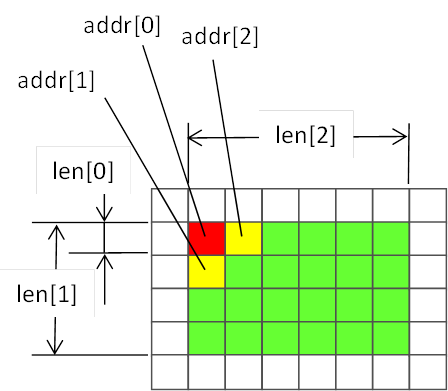
\includegraphics[]{research/sato/fig1.png}
  \caption{Parameters that determines data contiguity}
  \locallabel{fig:fig1}
\end{figure}

\subsubsection{Experimental Results}

\begin{description} 

\item[(1) Himeno benchmark] \ \\

We ported Himeno benchmark program written with MPI to four different CAF programs. They used the same Fujitsu Fortran compiler with the same options including automatic thread parallelization. While the MPI version has 610 lines excluding comment and empty lines, the CAF versions have 402 to 415 lines, 32\% to 34\% shorter.

The result on grid size XL (1024   512   512) is shown in Figure \localref{fig:fig2}. Two CAF programs are respectively 5\% and 2\% faster than the MPI version in average.

\begin{figure}
\centering
  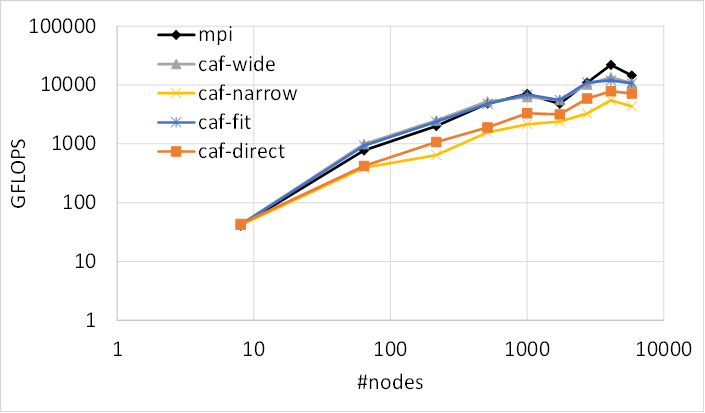
\includegraphics[]{research/sato/fig2.png} 
  \caption
{Four different CAF programs vs. the original MPI on Himeno benchmark}
  \locallabel{fig:fig2}
\end{figure}

\item [ (2) NAS Parallel benchmark ] \ \\

We ported NAS Parallel benchmarks CG, EP, FT and MG written in MPI for CAF respectively. Figure \localref{fig:fig3} shows the result of CG Class-C as an instance and summarizes the history of the CAF program tuning. Finally CAF program V49 exceeds the original MPI version in performance. On EP, the CAF version is only 2\% less performance in average than the original without tuning. On FT, the first version of CAF program extract more than 93\% of the performance of the original in all evaluation ranges of Class B, C and D. Besides the CAF program has still room for performance tuning. On MG, the final version of CAF provides almost the same performance as the original in average.

\begin{figure}
\centering
  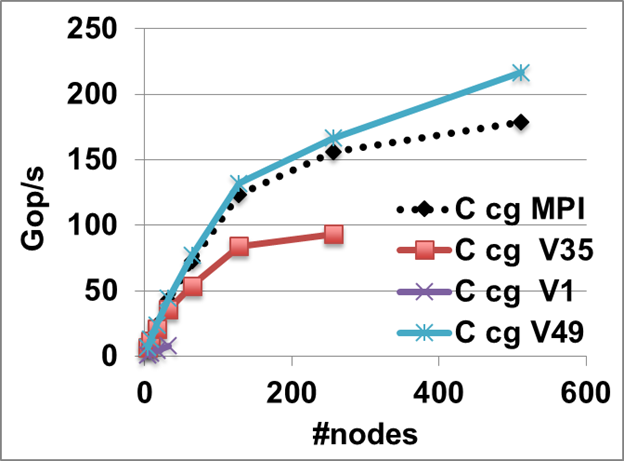
\includegraphics[]{research/sato/fig3.png} 
  \caption {Porting and performance tuning of CAF program on NPB CG Class-C}
  \locallabel{fig:fig3}
\end{figure}

\end{description}

\subsection{ Performance Evaluation of the HPC Challenge Benchmark with XcalableMP}

To evaluate productivity and performance of XcalableMP, we have implemented four benchmarks, namely STREAM, HPL, FFT, RandomAccess, in the HPC Challenge Benchmark Suite by using XcalableMP. 

The figure \localref{fig:fig4} shows that the performance results of the XMP implementations. For a comparison purpose, we have also evaluated the performances of the MPI implementations which are reference implementations. The horizontal axis means that the number of compute nodes, the left vertical axis means that the performance corresponding to the bar, the right vertical axis means that the ratio of the performance of the XMP implementation to that of the MPI implementation corresponding to the line. When the performance ratio is greater than 1, the performance of the XMP implementation is better than that of the MPI implementation. The figure shows that the performances of XMP are almost the same as those of MPI.

\begin{figure}
\centering
  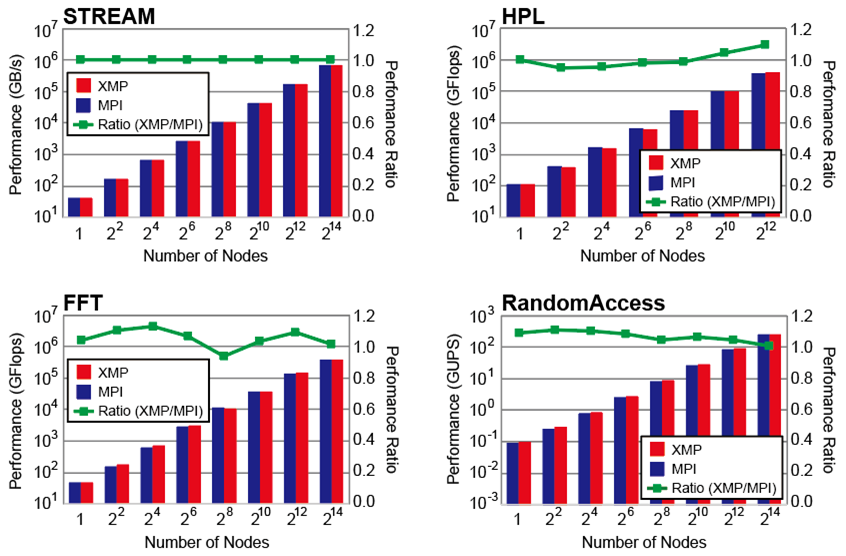
\includegraphics[width=1.0\textwidth]{research/sato/fig4.png}
  \caption{Performance of HPC Challenge Benchmark with XcalableMP}
  \locallabel{fig:fig4}
\end{figure}


The table \localref{tbl:table1}  shows that source lines of code (SLOC) of the benchmarks in XMP and MPI. The table shows that the SLOCs of the XMP implementations are much less than those of the MPI implementations.

\begin{table}
\centering
  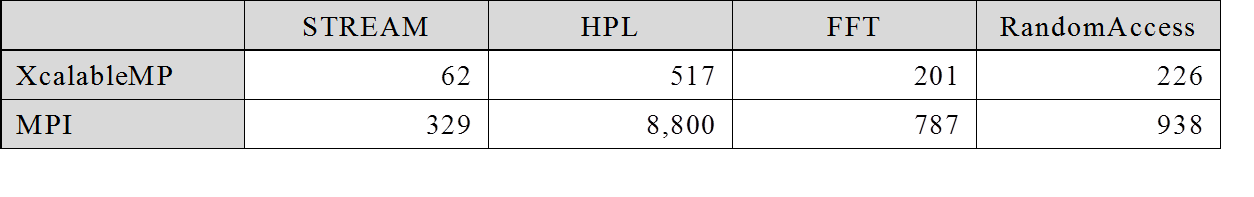
\includegraphics[width=0.9\textwidth]{research/sato/table1.png}
  \caption{SLOC of HPC Challenge Benchmark with XcalableMP}
  \locallabel{tbl:table1}
\end{table}

\subsection { Performance of Three-dimensional Fluid Simulation with XcalableMP
}

The three-dimensional Eulerian fluid code written in Fortran,
IMPACT-3D, which performs compressible and inviscid fluid computation
to simulate converging asymmetric flows related to laser fusion, is
parallelized by three different domain decomposition methods, namely
the domain is divided in (1) only Z direction, (2) both Y and Z
directions and (3) all of X, Y and Z directions using by using
directives only for the “global-view” programming model of
XcalableMP (XMP). The program is also hand-coded with MPI using
the same domain decomposition methods, and the performance difference
between XMP and MPI codes is evaluated on the K computer.

As one node consists of 8 cores in the K computer, one process is
dispatched onto each node and each process performs parallel
computations with 8 threads, which are explicitly described by OpenMP
in both XMP and MPI programs. We run both XMP and MPI codes with three
different decomposition methods and evaluate the weak scaling on the K
computer using Omni XcalableMP/Fortran compiler 0.7.0 and Fujitsu
Fortran K-1.2.0.15. A number of cores for execution and corresponding
simulation parameters are summarized in Table \localref{tbl:table2}. lx, ly, lz are
Fortran array size of first, second, third dimension, and nx, ny, nz
are a number of division in X, Y, Z direction, respectively.

\begin{table}
\centering
  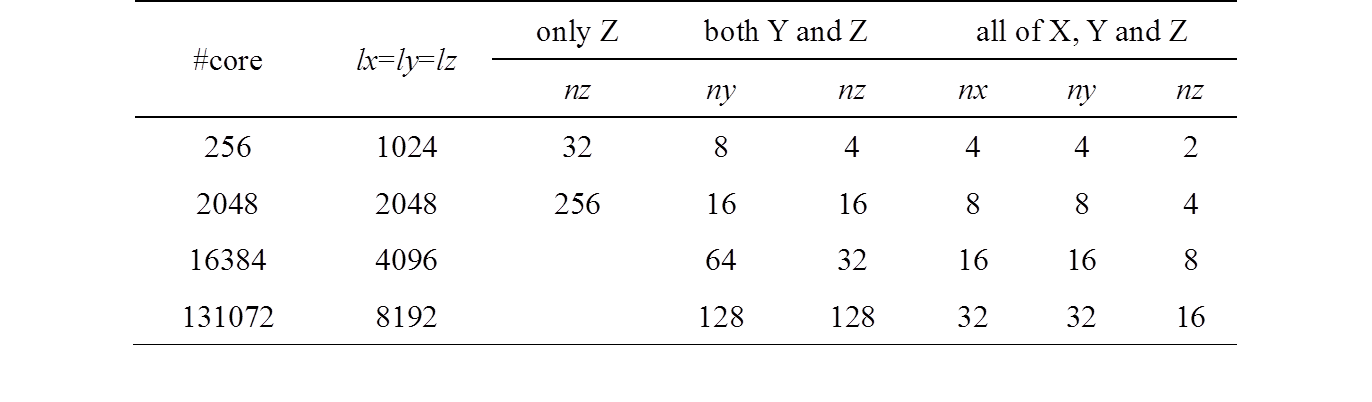
\includegraphics[width=0.9\textwidth]{research/sato/table2.png}
  \caption{Simulation parameters}
  \locallabel{tbl:table2}
\end{table}

Performance is measured by a hardware monitor installed on the K computer, and three indexes are obtained. The total number of floating point operations is counted by the hardware monitor and is interpreted to MFLOPS using elapsed time. Finally it is divided by theoretical peak MFLOPS and output as MFLOPS/PEAK value. The average amount of transfer data per second between memory and CPU is also monitored. It is divided by theoretical peak memory access throughput and output as Memory throughput/PEAK value. The hardware monitor counts the number of instructions, and the number of SIMD instructions is divided by the total number of instructions to obtain SIMD execution usage.

MFLOPS/PEAK values for all 6 cases, namely (MPI, XMP) x (only Z, both Y and Z, all of X, Y and Z) are shown in Fig. \localref{fig:fig5} (a). Performance of XMP codes is as same as that of MPI codes, and small differences among three decomposition methods are found. But we can get only 8 ~ 9 \% of peak performance of the K computer. From the hardware monitor, we found that SIMD execution usage was less than 5\% in all cases, and this could degrade the performance. Most cost intensive DO loops in IMPACT-3D include IF statements, which are needed to correctly treat extremely low velocity and flow direction change regardless of XMP and MPI codes, and the IF statement prevents the native Fortran compiler from generating SIMD instructions inside the DO loop. Thus relatively low performance is obtained.

As the true rate of the IF statement is nearly 100\% in IMPACT-3D, speculative execution of SIMD instruction causes almost no overhead. So forcing the compiler to generate the SIMD instructions could be useful to enhance the performance, and it can be done with “simd=2” compiler option. All codes are recompiled with that option and rerun. SIMD execution usage increases up to around 50\% in all cases, and we can expect performance improvement. MFLOPS/PEAK values for all cases are shown in Fig. \localref{fig:fig5} (b). MPI code performance is improved and we can get up to 20\% of the peak performance. XMP code performance is also improved, but these are below 15\% even XMP code performance is almost same as MPI code performance without “simd=2” option. Although Memory throughput/PEAK values of MPI codes are 55\%, those of XMP codes are only 37\% and this low memory throughput is one of candidates for low sustained performance.

In the converted code by the XMP/F compiler, all Fortran arrays are treated as allocatable arrays even the original code uses static arrays. The allocatable array prevents the native Fortran compiler from optimizing the DO loop with prefetch instructions because the array size cannot be determined at compilation time, and it could cause low memory throughput. All Fortran static arrays in the hand-coded MPI code for the decomposition method of all of X, Y and Z directions are just replaced by allocatable arrays and we check a performance difference. Performance of the MPI code is shown in Fig. \localref{fig:fig5} (c) for static arrays (blue dash) and allocatable arrays (purple dash). MFLOPS/PEAK values are dropped from 20\% to 15\%, and this performance degradation without the prefetch instructions is confirmed. To force the native Fortran compiler to perform the prefetch optimization, we can use additional “prefetch\_stride” compiler option. All codes are recompiled with “simd=2” and “prefetch\_stride” options and rerun. Performance improvements by this compiler option are shown in Fig. \localref{fig:fig5} (c) for both MPI (purple dash to red dash) and XMP (purple solid to red solid) codes. MFLOPS/PEAK values are improved by 2 ~ 3\% with the prefetch optimization.

\begin{figure}
\centering
  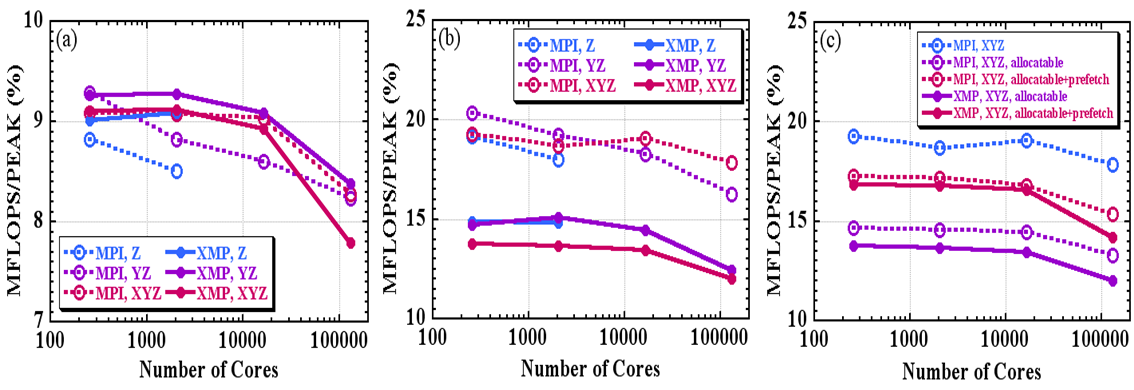
\includegraphics[width=1.0\textwidth]{research/sato/fig5.png}
  \caption{Performance comparison between MPI and XMP on the K computer with (a) no optimization for three decomposition methods, (b) SIMD optimization for three decomposition methods and (c) allocatable array optimization for the decomposition method of all of X, Y and Z directions.}
  \locallabel{fig:fig5}
\end{figure}

\subsection {Design of SCAMP (SCAlable Mpi Profiler) as a co-design tool for large-scale network}

Co-design for HPC is a bidirectional approach, where a system would be designed on demand from applications, and applications must be optimized to the system. In order to co-design the network of large scale systems, it is important to evaluate the communication performance of applications. The trace driven simulator estimates the network performance based on trace files. Firstly, user should run their application on a real system in parallel to obtain the trace files from all processes. These trace files should contain MPI function calls, and their arguments and time stamps, etc. Then, the performance of a virtual system is estimated by using the trace files. While the trace driven simulator is straightforward, sometimes it is not appropriate for the simulation of large parallel systems since it is difficult to obtain the number of trace files for the future system if the current system is smaller than the future one. In order to tackle this scaling-problem in the trace driven simulator, we propose a method called SCAMP (SCAlable Mpi Profiler), which creates a large number of pseudo trace files based on the small number of trace files obtained from a small system and drives the network simulator using the pseudo trace files to estimate the performance of the large systems. 

According to the experiments using SCAMP and using K-computer, as shown in Figure \localref{fig:fig7}, SCAMP overestimates the performance of benchmarks, i.e. the runtime estimated by SCAMP is shorter than the real runtime on K-computer. The reason is that while we have focused only on the network performance, the computation time would change as the number of nodes increases.

\begin{figure}
\centering
  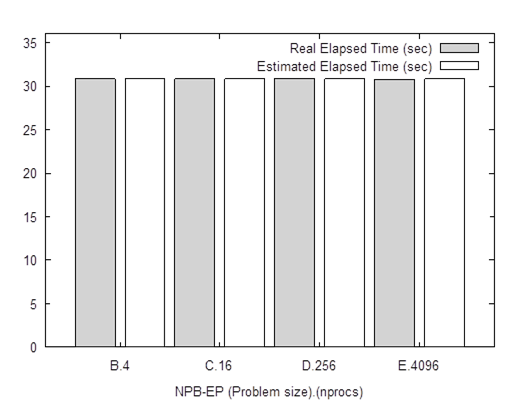
\includegraphics[width=0.45\textwidth]{research/sato/fig6.png}
  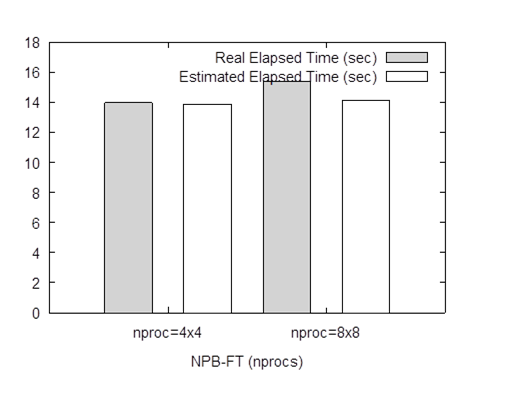
\includegraphics[width=0.5\textwidth]{research/sato/fig7.png}
  \caption{Comparison between real time and estimated time by SCAMP}
  \locallabel{fig:fig7}
\end{figure}

\subsection{Performance evaluation of Tascell on the K computer}
 
Tascell is a task parallel language that supports distributed memory environments. A Tascell worker spawns a real task only when requested by another idle worker. The worker spawns a task after restoring its oldest task-spawnable state by temporarily backtracking. This mechanism eliminates the cost of spawning/managing logical threads. It also promotes the reuse of workspaces and improves the locality of reference since it does not need to prepare a workspace for each concurrently runnable logical thread. Furthermore, a single Tascell program can run efficiently on shared and distributed memory environments.

This study aims to evaluate Tascell on massively parallel systems; in particular, we employed 1024 nodes of the K Computer with 8192 cores in total. In addition, we revised the implementation of Tascell to get it working on such systems.

In the conventional implementation of Tascell, inter-node communication is realized by TCP/IP communication via message routing servers called Tascell servers. This implementation is suitable for dynamic addition of computation nodes and wide-area distributed environments. On the other hand, Tascell servers often become communication bottlenecks. Furthermore, in recent supercomputer environments, there may be no appropriate places for deploying Tascell servers, and TCP/IP may not be available for inter-node communication; it is hard or impossible to run the conventional implementation in such an environments.

Therefore, we implemented inter-node communication in Tascell using MPI, which is supported by most practical supercomputer systems. At the same time, we adopted a server-less implementation in order to overcome the deployment and bottleneck problems, excluding the support of wide-area distributed environments. Note that programmers can write Tascell programs without concern about the underlying communication layer.

We evaluate the performance of our MPI-based implementation on the K computer using 7168 workers (7 workers x 1024 nodes).
The result is shown in Figure \localref{fig:fig8}.

In order to enable our implementation to work with the MPI implementation on the K computer and many other MPI implementations, it only requires the MPI\_THREAD\_FUNNELED support level, in which only the main thread can make MPI calls, and the two-sided communication paradigm. With such minimum requirements, our MPI-based implementation successfully realized both high performance and deadlock freedom.

\begin{figure}
\centering
  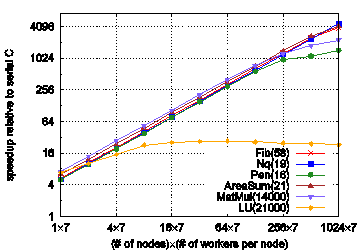
\includegraphics[width=0.9\textwidth]{research/sato/fig8.png}
  \caption{Evaluation results (Speedup) of Tascell programs on the K computer}
  \locallabel{fig:fig8}
\end{figure}

\section{Schedule and Future Plan}

From this year, we started the study of the programming models for post-petascale, including programming models and runtime techniques to support manycore. We already propose XcableACC as a solution for accelerator-based system, which is to be explored in the JST CREST project. As the post-K computer will be a large-scale multicore-based system, we will investigate programming models for manycore-based parallel systems including dynamic tasking and load balancing as well as advanced PGAS models for distributed memory systems.

As in recent years, an important action for XcalableMP project is to disseminate our XcalableMP to applications users. As in last years, we organized several schools and hands-on, workshop with potential users also in this year. We will continue these promotion activities while we will study more optimization technique of XcalableMP compiler to improve the performance. As a research agenda especially for the K computer, we will contribute the scalability of large-scale applications for the K computer.

%%% DO NOT EDIT BELOW

\section{Publications}

%\printbibliography[keyword=journal, heading=subbibliography, title={Journal Articles}, prefixnumbers={1-}, resetnumbers=true]
%\printbibliography[keyword=proceedings, heading=subbibliography, title={Conference Papers}, prefixnumbers={2-}, resetnumbers=true]
%\printbibliography[keyword=invited, heading=subbibliography, title={Invited Talks}, prefixnumbers={3-}, resetnumbers=true]
%\printbibliography[keyword=poster, heading=subbibliography, title={Posters and Presentations}, prefixnumbers={4-}, resetnumbers=true]
%\printbibliography[keyword=deliverable, heading=subbibliography, title={Patents and Deliverables}, prefixnumbers={5-}, resetnumbers=true]

\printbibliography[keyword=journal, heading=subbibliography, title={Journal Articles}, resetnumbers=true]
\printbibliography[keyword=proceedings, heading=subbibliography, title={Conference Papers}]
\printbibliography[keyword=invited, heading=subbibliography, title={Invited Talks}]
\printbibliography[keyword=poster, heading=subbibliography, title={Posters and Presentations}]
\printbibliography[keyword=deliverable, heading=subbibliography, title={Patents and Deliverables}]

\end{refsection}

%\begin{refsection}[research/taiji/group.bib]
\nocite{*}
\chapter{Processor Research Team}

\section{Members}

\begin{itemize}
  \item[] Ichiro Kobe (Team Leader)
  \item[] Jiro Kobe (Senior Scientist)
  \item[] Saburo Kobe (Research Scientist)
\end{itemize}

\section{Research Activities}

Text for research activities.

\section{Research Results and Achievements}

Text for research Results and achievements. Journal-artcile~\cite{sample-journal}.
Conference-paper~\cite{sample-conference}.
Invited-talk~\cite{sample-invited}.

For cross referencing, use \verb|\locallabel| and \verb|\localref| to avoid conflicting names defined by other groups. For example, a figure can be referenced as Figure~\localref{fig:sample-label1}.

\begin{figure}
\centering
  
\includegraphics[width=0.5\textwidth,keepaspectratio,natwidth=193,natheight=40]
  {sample_division/sample_group/test1.png}
  \caption{Caption for a sample figure}
  \locallabel{fig:sample-label1}
\end{figure}

\section{Schedule and Future Plan}

Text for schedule and future plan.

%%% DO NOT EDIT BELOW

\section{Publications}

%\printbibliography[keyword=journal, heading=subbibliography, title={Journal Articles}, prefixnumbers={1-}, resetnumbers=true]
%\printbibliography[keyword=proceedings, heading=subbibliography, title={Conference Papers}, prefixnumbers={2-}, resetnumbers=true]
%\printbibliography[keyword=invited, heading=subbibliography, title={Invited Talks}, prefixnumbers={3-}, resetnumbers=true]
%\printbibliography[keyword=poster, heading=subbibliography, title={Posters and Presentations}, prefixnumbers={4-}, resetnumbers=true]
%\printbibliography[keyword=deliverable, heading=subbibliography, title={Patents and Deliverables}, prefixnumbers={5-}, resetnumbers=true]

\printbibliography[keyword=journal, heading=subbibliography, title={Journal Articles}, resetnumbers=true]
\printbibliography[keyword=proceedings, heading=subbibliography, title={Conference Papers}]
\printbibliography[keyword=invited, heading=subbibliography, title={Invited Talks}]
\printbibliography[keyword=poster, heading=subbibliography, title={Posters and Presentations}]
\printbibliography[keyword=deliverable, heading=subbibliography, title={Patents and Deliverables}]

\end{refsection}

\begin{refsection}[research/imamura/group.bib]
\nocite{*}
\chapter{Large-Scale Parallel Numerical Computing Technology Research Team}

\section{Members}

\begin{itemize}
  \item[] Toshiyuki Imamura (Team Leader)
  \item[] Yoshiharu Ohi (PostDoctoral Researcher)
  \item[] Yusuke Hirota (PostDoctoral Researcher)
  \item[] Daichi Mukunoki (PostDoctoral Researcher)
  \item[] Daisuke Takahashi (Senior Visiting Researcher)
  \item[] Franz Franchetti (Visiting Researcher)
  \item[] Yoshio Okamoto (Visiting Researcher)
  \item[] Takeshi Fukaya (Visiting Researcher)
  \item[] Cong Li (Student Trainee)
  \item[] Doru Thom Popovich (Student Trainee)
  \item[] Yukiko Akinaga (Assistant)
\end{itemize}

\section{Research Activities}

The Large-scale Parallel Numerical Computing Technology Research Team conducts research and development of large-scale, highly parallel and high-performance numerical software for K computer. Simulation programs require various numerical techniques to solve systems of linear equations, to solve eigenvalue problems, to compute and solve non-linear equations, and to do fast Fourier transforms. In order to take advantage of the full potential of K computer, we must select pertinent algorithms and develop a software package by assembling numerical libraries based on the significant concepts of high parallelism, high performance, high precision, resiliency, and scalability.
Our primary mission is to develop and deploy highly parallelized and scalable numerical software on K computer, namely KMATHLIB. It comprises several components such as for solving
\begin{itemize}
\item systems of linear equations,
\item eigenvalue problems,
\item singular value decomposition,
\item fast Fourier transforms, and
\item nonlinear equations.
\end{itemize}
The K-specific topics and technical matters for emerging supercomputer systems are also our challenging works such as
\begin{itemize}
\item Tofu interconnect,
\item parallel I/O,
\item fault detection (soft-error), and
\item higher accuracy computing.
\end{itemize}

We are going to complete this project through a tight collaboration among computational science (simulation), computer science (hardware and software), and numerical mathematics. Our final goal is to establish fundamental techniques to develop numerical software libraries for next generation supercomputer systems based on strong cooperation within AICS.

\section{Research Results and Achievements}

Following series of the annual reports from 2012-13 to 2014-15, we summarize the latest results of our running projects, mainly focused on 1) development of KMATHLIB, 2) development of EigenExa, 3) investigation of FDTD related methods, and 4) other fundamental studies to optimize the BLAS kernels through automatic parameter tuning. The plans and the publication list are also presented in the last section.

\subsection{KMATHLIB Project}

\subsubsection{Development of KMATHLIB for the integration of OSS packages}

Since FY2012-2013, we have developed an integration framework named KMATHLIB, which supports a broad range of numerical libraries, and its API covers the computation resources from hundreds of nodes to the whole system of K computer.

\begin{figure}
\centering
  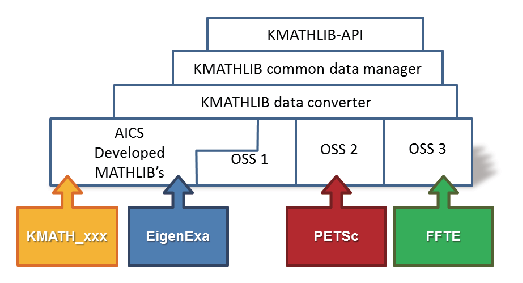
\includegraphics[width=0.66\textwidth,keepaspectratio,natwidth=193,natheight=40]
  {research/imamura/KMATHLIB_API.eps}
  \caption{Software layer of KMATHLIB}
  \locallabel{fig:Fig1}
\end{figure}

Fig. \localref{fig:Fig1} draws the schematic of KMATHLIB. KMATHLIB API is on the top layer and is accessed by users directly. Since we designed a flexible plugin mechanism and APIs, favorite OSS can be plugged in like the bottom highlighted part of Fig. \localref{fig:Fig1}. We intended to develop KMATHLIB API so that it encapsulates any components related to the libraries and conceals the differences of APIs and data structures. KMATHLIB API adopts a modern API style of the standard numerical libraries, like PETSc and FFTE. Thus, we only have to use a unique procedure to use the numerical solver plugged in the KMATHLIB package. In this FY2015-2016, we have updated the plugin mechanism to enable users to enhance the KMATHLIB library according to their computational environment  \cite{EigenExa,KMATH-EIGEN-GEV,KMATH-RANDOM}.

\subsubsection{Maintenance and modification of KMATHLIB API}

In FY2015, as a part of KMATHLIB project, we developed KMTHLIB API. KMATHLIB API is an application programming interface for development of computational science software. It provides a common interface and related functions for using various numerical libraries to reduce the cost of the development and maintenance of computational science software. Based on application and investigation on real simulation codes\cite{JKIS-JCPC2016, MSII-MC+SNA+MC2015}, the mechanism of software plugin and kernel functions are designed and implemented. The current KMATHLIB API contains the user interface and functions to use several basic (built-in) numerical libraries.

In March 2016, we organized a tutorial program for the KMATHLIB project, and the KMATHLIB API was available on a Fujitsu FX10 computer at that time.
In the end, the tarball and user's manual of KMATHLIB API has been released (23 May, 2016) \cite{KMATHLIB-API}.

\subsubsection{Feasibility study of asynchronous algorithms for applied mathematics}

The asynchronous algorithms and their representation methods have been investigated as a part of research on the development of algorithms for manycore processors. In FY2015, we have investigated some conventional asynchronous algorithmi, including the incomplete LU factorization algorithm proposed by E. Chow et al., a Jacobi/Gauss-Seidel like algorithm, and a logic of parallel adders, We classified the algorithms into two groups: (1) algorithms based on the approximation of operators and (2) algorithms which represent the original solution with the ones of other problems. Base on the classification, we derived a new back substitution algorithm of a narrow banded matrix for manycore processors. We carried out preliminary experiments on an Intel Xeon Phi 3120P, which show that the derived algorithm achieved 1.8 times speedup over a sequential implementation of the DTBSV of Intel Math Kernel Library in the case of a $32\times10^6$ dimensional band matrix with bandwidth 3 (shown in Fig. \localref{fig:Fig2}).

\begin{figure}
\centering
  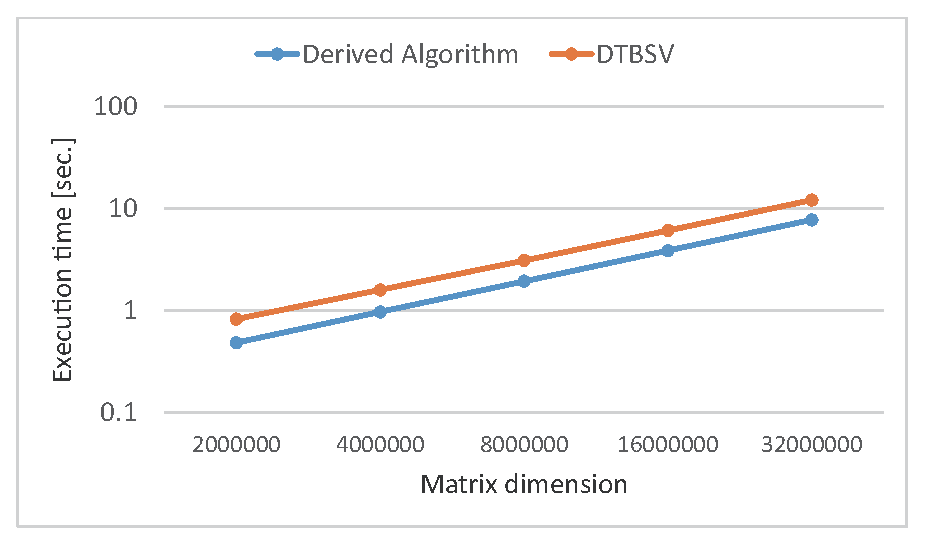
\includegraphics[width=0.66\textwidth,keepaspectratio,natwidth=193,natheight=40]
  {research/imamura/DTBSV-2.eps}
  \caption{The execution time of DTBSV in Intel Math Kernel Library and the implementation of the derived algorithm}
  \locallabel{fig:Fig2}
\end{figure}

\subsubsection{A solver for generalized eigenvalue problems of banded matrices}

We have researched on the solver for generalized eigenvalue problems of banded matrices (GEPBs) since FY2013-2014. In FY2015-2016, we studied techniques to implement the algorithm proposed in FY2014-2015 for manycore systems. We implemented communication hiding technique on an Intel Xeon Phi system and evaluated its performance.
%
Fig. \localref{fig:Fig3} shows that
the implementation run on `a CPU(16threads) + a Xeon Phi' outperforms the routine DSYGVD, a de facto standard numerical library, run on `a CPU(16threads)' about 7.1 times by elapsed time.
%
Also, the simultaneous use of a CPU and a Xeon Phi accelerates the performance 2.2 times over the single use of a CPU.
%
The related results were presented in the SIAM LA \cite{HI-SIAMLA2015} and EPASA \cite{HI-EPASA2015} as oral and poster presentations in 2015, respectively.

\begin{figure}
\centering
  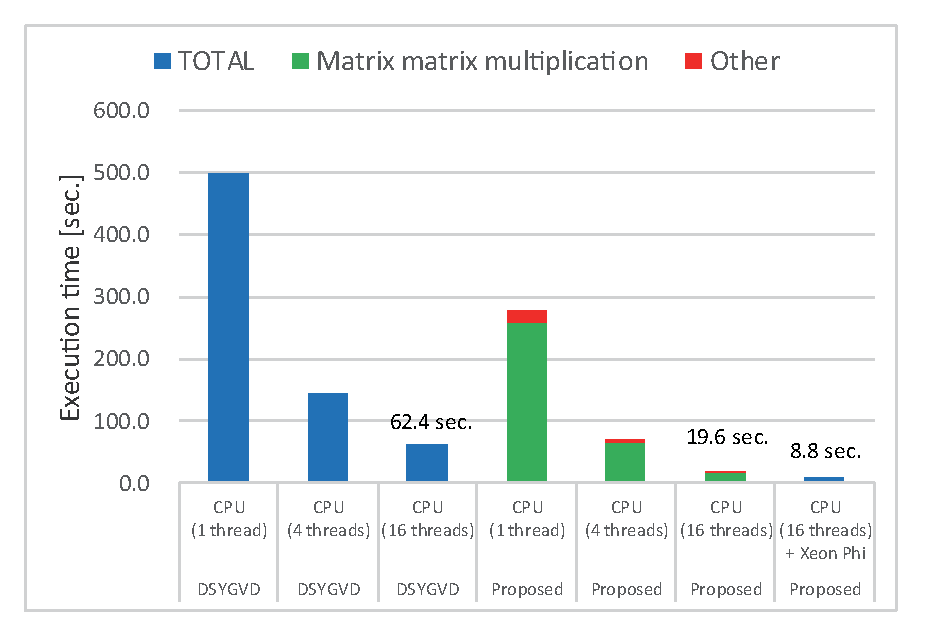
\includegraphics[width=0.66\textwidth,keepaspectratio,natwidth=193,natheight=40]
  {research/imamura/bandEigen.eps}
  \caption{The execution time of DSYGVD and the implementations of the proposed algorithm for a CPU, and the implementation for an Intel Xeon Phi system. The test matrix is a 10,000-dimensional random matrix.}
  \locallabel{fig:Fig3}
\end{figure}


\subsection{EigenExa Project}

We conducted the EigenExa Project with the grant support of `Development of System Software Technologies for post-Peta Scale High Performance Computing' by JST CREST (the project code name was `Development of an Eigen-Supercomputing Engine using a Post-Petascale Hierarchical Model' and the leader was Prof. Tetsuya Sakurai, University of Tsukuba) during FY2010-FY2015. In FY2015-16, we concluded our EigenExa project, on which we developed a parallel dense eigenvalue solver. The EigenExa library was already released in August 2013, and the current release version is 2.3d (31 August 2015).

Following FY2014-2015, we continued to promote the library and evaluated the performance on some available supercomputer systems, such as a Fujitsu FX10, an NEC SX-ACE, an IBM BlueGene/Q, and Intel Cluster systems. In the performance evaluation, we reported the preprocessing part of tri-diagonalization and pent-diagonalization at PDSEC2015 \cite{FI-PDSEC2015}, and the divide and conquer part at EPASA2015 \cite{FI-EPASA2015}.

\subsubsection{Communication avoiding algorithm for the Householder tri-diagonalization}

Communication avoidance (CA) is considered to be a promising technology to overcome the drawbacks resulting from the communication latency. Well-known examples of the CA algorithm reported in the literature are the tall skinny QR decomposition (TSQR) algorithm and the matrix powers kernel (MPK) algorithm. We investigated the related algorithm CholQR2, and showed a policy or a sort of new performance metric of the Chebyshev basis conjugate gradient (CBCG) method on K computer \cite{KFTHFIS-PPAM2015}.

Even though the CA algorithms induce more flops counts, the CA algorithms tend to reduce the number of communication, which is often dominant part of parallel computing on modern systems. To derive a new communication avoiding Householder scheme, we applied two simple principles (or simple rule) for transformation; i) distributive property of linear operators, ii) combining a couple of communication into one.
In Fig \localref{fig:Fig4}, the underlined statement requires two \verb+MPI_Allreduce+'s per iteration. This is the optimal version because matrix-vector multiplication needs at least two collective communications when we take advantage of the symmetric property of the matrix. Since the naive Householder tridiagonalization has to call five \verb+MPI_Allreduce+'s per iteration, the proposed version drastically reduces the number of communications and leads to better parallel scalability. The proposed algorithm CAHTR(3) was presented in ParCo2015 conference\cite{IFHYM-ParCo2015}, and Communication Hiding (CH) technique was also presented at SIAM LA 2015 \cite{I-SIAMLA2015}. At the moment, the parallel implementation of the present version 2.3 or later yields good performance acceleration on K computer compared with the non-CA/CH optimized version (see Fig. \localref{fig:Fig4_2}).

\begin{figure}
\centering
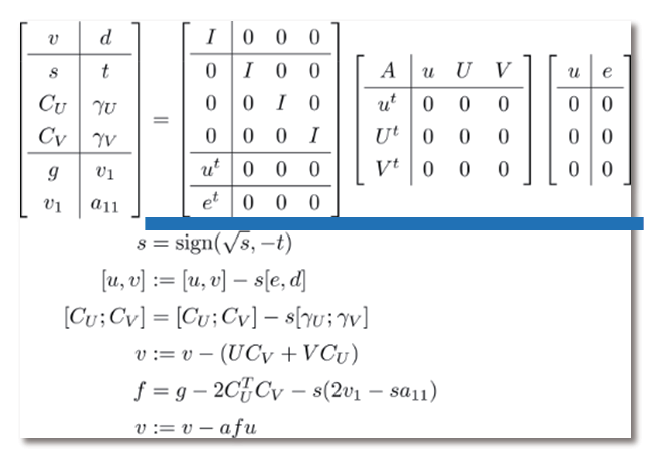
\includegraphics[width=0.66\textwidth,keepaspectratio,natwidth=193,natheight=40]
  {research/imamura/CAHTR_3.eps}
  \caption{Communication avoiding Householder tridiagonal transformation}
  \locallabel{fig:Fig4}
\end{figure}

\begin{figure}
\centering
  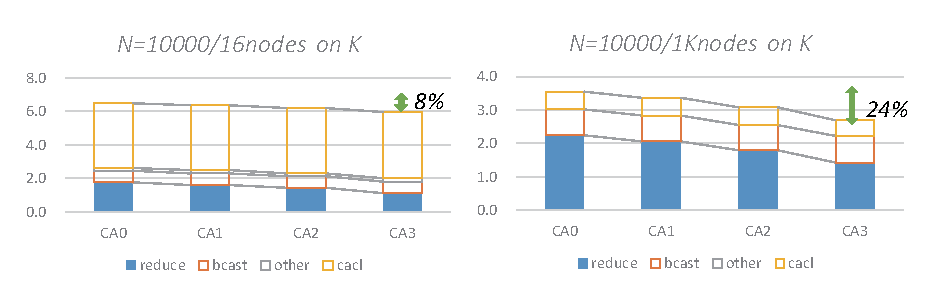
\includegraphics[width=\textwidth,keepaspectratio,natwidth=193,natheight=40]
  {research/imamura/CAHTR_on_K.eps}
	\caption{Big impact of performance improvement by CAHTR (Communication Avoiding Householder TRidiagonalization). The blue bars correspond to the elapsed time of \texttt{MPI\_{}Allreduce} operations.}
  \locallabel{fig:Fig4_2}
\end{figure}


\subsection{Investigation of the FDTD Related Methods}

\subsubsection{FDTDM (Finite-Difference Time-Domain Method)}

Since electronic apparatuses downsize in a short period and the cost-cut of development is strongly demanded, numerical simulation is thought to be useful to a industrial design process.
%
High definition and large-scale simulations must be indispensable for reliable evaluation.
%
The finite-difference time-domain method (FDTDM) is applied for numerical simulations of electromagnetic wave propagation phenomena, while most of the preexistent software of FDTDM are commercial.
%
Modification to the software or change of a simulation scenario sometimes are limited due to the software licencing.
%
Therefore, we decided to develop open source software based on FDTDM for K computer.
%
Since FY2014-2015, we have surveyed the computational electromagnetics and social contribution of numerical simulation by using FDTDM and related methods.


\subsubsection{MTDM (Meshless Time-Domain Method)}

In the simulation using FDTDM, the node arrangement of the electric and magnetic fields based on a staggered grid often becomes a significant difficulty when we treat a complex shaped domain including a curved surface.
%
The hybrid idea of FDTDM and a meshless method yields a novel spatial discretization scheme of the meshless time-domain method (MTDM).
%
The meshless method is a mathematical approach to find an approximate solution of the boundary value problem of the partial differential equation without using the grid which is used in the finite element method.
%
Therefore, it is expected that analysis of electromagnetic wave propagation phenomena in a complex shaped domain can be easily executed by using MTDM.
%
In FY2015-2016, we developed a test version of the three-dimensional MTDM simulator \cite{OI-PFR2015}.
%

\subsection{A study for development of high-performance linear algebra libraries on future architectures}

Traditional linear algebra libraries such as Basic Linear Algebra Subprograms (BLAS) are still important building blocks for computational science. 
As processor architectures become more and more complex, more challengings on development and code optimization are met. Also, they are required not only to achieve high performance, but also to support accurate, fault-tolerant, and energy-efficient computations toward the Exascale computing. Therefore, we are conducting a study for developing such linear algebra kernels on modern many-core architectures such as GPUs. 

\subsubsection{High performance memory-bound BLAS routines with automatic thread-block size adjustment on CUDA}

In the previous FYs, we proposed a sophisticated implementation of general and symmetric matrix-vector multiplication (GEMV and SYMV) routines on CUDA \cite{ASPEN.K2,MUBLAS-GEMV}.  
In this FY2015-2016, we have extended the study to other memory-bound linear algebra kernels \cite{MIT-HPC150, IMYM-HPC151}. The performance of CUDA kernels often depends on the number of threads per thread-block (thread-block size), and the optimal thread-block size often differs according to the GPU hardware running the kernel and the given data size to the kernel. We proposed a method to determine the nearly optimal thread-block size for the DGEMV kernel. Our proposed method automatically and theoretically determines the thread-block size using an occupancy model for thread-blocks on a grid along with warp-occupancy and some rules (Fig. \localref{fig:Fig5}),
Also, we improved and extended our GEMV and SYMV implementations to support multi-GPU environments. Our implementations, especially GEMV kernels, achieved better throughput and performance stability with respect to the matrix size on up to 4 Kepler GPUs when compared to the existing implementation
\begin{figure}
\centering
  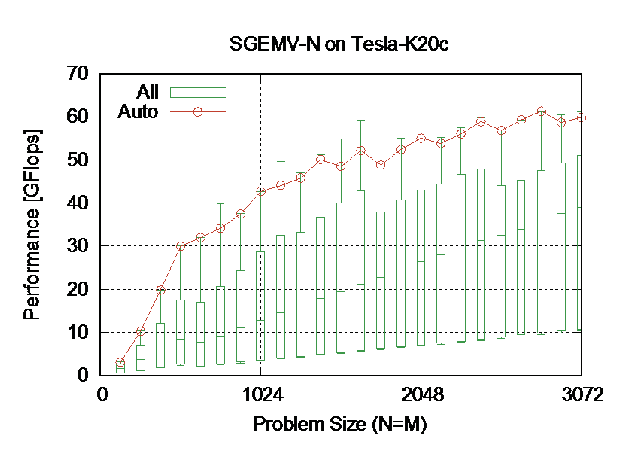
\includegraphics[width=0.66\textwidth,keepaspectratio,natwidth=193,natheight=40]
  {research/imamura/MUBLAS.eps}
  \caption{Performance of SGEMV-N (single-precision, non-transposed) on Tesla K20c Kepler GPU. The green line (All) shows the performance distribution obtained by all possible configurations of thread-block size. The red line (Auto) shows the performance obtained by our method.}
  \locallabel{fig:Fig5}
\end{figure}

\subsubsection{Short length floating-point formats (SLFP) for fast and energy efficient computation (work-in-progress)}

The required precision depends on the purpose of the computation. However, most numerical libraries only support IEEE754 32- and 64-bit floating point formats. To optimize the performance of numerical software prominently with respect to the precision, we proposed new floating-point formats that have shorter bit-length than IEEE standards on both CPUs and GPUs \cite{MI-HPC152}. By eliminating waste data movement in the computation using the shorter floating-point formats, we expect to improve the computation speed and energy efficiency. In our preliminary evaluation on a GPU, the proposed method achieved better performance and energy efficiency. A preliminary version is available from our webpage \cite{SLFP}.

\subsection{Seminar}
We hosted researchers from foreign research institutes, and organized a part of AICS HPC seminars in this FY2015-2016 (see also the webpage \url{https://sites.google.com/site/aicshpcseminar/}).
\begin{itemize}
\item 4-{th} AICS HPC Seminar, Friday, September 11, 2015,
\begin{enumerate}
\item Cong Li (the Department of Computer Science at the University of Tokyo (Ph.D. student)), `Evaluation of Communication-Avoiding Block Chebyshev Basis Conjugate Gradient Method Based On Large Scale Experiment'
\item Prof. Bruno Lang (Computer Science (Algorithms) at University of Wuppertal), `High-performance large-scale eigenvalue computations'
\end{enumerate}
\item 7-{th} AICS HPC Seminar, Tuesday, March 29, 2016,
\begin{enumerate}
\item Dr. Osni Marques (Lawrence Berkeley National Laboratory, US), 'Tuning the Coarse Space Construction in a Spectral AMG Solver'
\item  Prof. Yusaku Yamamoto (The University of Electro-Communications, Japan), `Roundoff Error Analysis of the CholeskyQR2 and Related Algorithms'
\item Dr. Susumu Yamada (Japan Atomic Energy Agency, Japan), `Quadrature precision basic linear algebra subprograms with FMA instruction and its applications'
\item Dr. Toshiyuki Imamura (RIKEN AICS, Japan), `EigenExa: Dense Symmetric eigenvalue solver for distributed parallel systems'
\end{enumerate}
\end{itemize}

\subsection{International Collaborations}

Our team has joined a new international project which runs on the Joint Laboratory for Extreme Scale Computing (JLESC) framework. The project is a collaboration with Inge Gutheil from Juelich Supercomputer Center (JSC) (\url{https://jlesc.github.io/about/}).
The title of the proposed project is `HPC libraries for solving dense symmetric eigenvalue problems', and we plan to evaluate the several aspects of the routines on the existing production and prototype supercomputers available to give the users recommendations which routine to use for their specific task.
In the 4th JLESC meeting in Bonn, December 2015, we had a pre-meeting of this project concerning a research update and planning in 2016 of each member.

At the 6-th AICS International Symposium in February 2016 at AICS, we also presented key research topics that would be potential themes for collaboration such as
\begin{enumerate}
\item application of EigenExa to application codes,
\item numerical algorithms, and
\item higher/reduced precision numerical kernels.
\end{enumerate}
In order to specify more detailed plans and roadmap for the collaborations,
we discussed with a couple of institutes that signed up MoU.


\section{Schedule and Future Plan}

\subsection{KMATHLIB project}

To promote KMATHLIB, the eternal maintenance of useful plugged-in OSS is of significance. From FY2014-2015, we extended plugin solvers such as for sparse linear equations, GEBPs, and SVD for tensors.
This FY2015-2016, we only did the investigation of the GEBPs solver on distributed highly parallel computers such as K computer due to the lack of human resources, whereas we will be able to release the solver package for GEBP as a part of KMATHLIB in FY2016-FY2017. In addition, we already completed the preliminary studies for the solver on many-core accelerators such as an Intel Xeon Phi, Knight Corner, aka KNC, thus, we are going to continue to study on both KNC and extend it to the emerging processor, an Intel Xeon Phi Knight Landing, aka KNL, in FY2016-2017.

\subsection{EigenExa project}

After the first release of the EigenExa library, several application codes adopt to use EigenExa. Continual maintenance of the EigenExa library becomes our important mission. In addition, the performance improvement and scalability towards the future systems such as a post-K computer. Even though, we introduced the Communication Avoiding (CA) and Communication Hiding (CH) techniques to the present EigenExa implementation, to apply these techniques to block algorithms must be established because other eigenvalue solver projects adopt this approach naturally.

Also, a lightweight or flexible implementation of BLAS kernels for small linear algebra is also an important issue. Through reviews to the application users on K computer system, major groups demand a very wide variety of spectrum and problem sizes.
Since the present version of EigenExa was intended to accelerate and scale up for the ultra-scale problem, we recognized to increase the performance on a diagonalization of a small dimension matrix, such as a couple of thousand dimensions.
Also, we will modify the EigenExa library to calculate not only full spectrum but a part of the spectrum, as other modern eigenvalue solvers do.

\subsection{FDTD related method}

One of the future works related to the FDTD project is to investigate the behavior of the three-dimensional MTDM scheme. In fact, we confirmed numerical errors in three-dimensional MTDM simulations when particular collocation point was selected.
Since the goal of MTDM is to apply for practical and industrial simulation codes, we recognize that it is significant to free numerical instability as well as to obtain performance improvement.
Also, we need to promote MTDM, which has been originally studied in our project.

\subsection{Other issues}

% check
In this annual report, we have untouched topics, fault tolerance (or resilience), and high precision computing such as double-double format computing. Some of these topics have been already investigated as one of the keywords for the petascale computing. For example, following issues were researched in previous FY's;
\begin{enumerate}
\item algorithmic-based fault torelance,
\item numerical reproducibility,
\item quad precision numerical tools, and
\item dynamical process mapping. 
\end{enumerate}
We are going to present them at international conferences soon.

In particular, we recognized that the research related to numerical precision, higher precision and reproducibility become important in near future.
The higher-precision numerical framework or software toolkit must be organized on modern or future supercomputer systems as well as the post-K computer.
For the feasibility study, we already have started research on a higher precision computational kernel of a spectral method \cite{SYMMI-JSIAM2015}. We will soon merge a higher-precision numerical library into KMATHLIB, and investigate the effect of numerical precision on real application codes.

% add mode if needed

%%% DO NOT EDIT BELOW

\section{Publications}

%\printbibliography[keyword=journal, heading=subbibliography, title={Journal Articles}, prefixnumbers={1-}, resetnumbers=true]
%\printbibliography[keyword=proceedings, heading=subbibliography, title={Conference Papers}, prefixnumbers={2-}, resetnumbers=true]
%\printbibliography[keyword=invited, heading=subbibliography, title={Invited Talks}, prefixnumbers={3-}, resetnumbers=true]
%\printbibliography[keyword=poster, heading=subbibliography, title={Posters and Presentations}, prefixnumbers={4-}, resetnumbers=true]
%\printbibliography[keyword=deliverable, heading=subbibliography, title={Patents and Deliverables}, prefixnumbers={5-}, resetnumbers=true]

\printbibliography[keyword=journal, heading=subbibliography, title={Journal Articles}, resetnumbers=true]
\printbibliography[keyword=proceedings, heading=subbibliography, title={Conference Papers}]
\printbibliography[keyword=invited, heading=subbibliography, title={Invited Talks}]
\printbibliography[keyword=poster, heading=subbibliography, title={Posters and Presentations}]
\printbibliography[keyword=deliverable, heading=subbibliography, title={Patents and Deliverables}]

\end{refsection}


\begin{refsection}[research/maeda/group.bib]
\nocite{*}
\chapter{HPC Usability Research Team}

\section{Members}

\begin{itemize}
  \item[] Ichiro Kobe (Team Leader)
  \item[] Jiro Kobe (Senior Scientist)
  \item[] Saburo Kobe (Research Scientist)
\end{itemize}

\section{Research Activities}

Text for research activities.

\section{Research Results and Achievements}

Text for research Results and achievements. Journal-artcile~\cite{sample-journal}.
Conference-paper~\cite{sample-conference}.
Invited-talk~\cite{sample-invited}.

For cross referencing, use \verb|\locallabel| and \verb|\localref| to avoid conflicting names defined by other groups. For example, a figure can be referenced as Figure~\localref{fig:sample-label1}.

\begin{figure}
\centering
  
\includegraphics[width=0.5\textwidth,keepaspectratio,natwidth=193,natheight=40]
  {sample_division/sample_group/test1.png}
  \caption{Caption for a sample figure}
  \locallabel{fig:sample-label1}
\end{figure}

\section{Schedule and Future Plan}

Text for schedule and future plan.

%%% DO NOT EDIT BELOW

\section{Publications}

%\printbibliography[keyword=journal, heading=subbibliography, title={Journal Articles}, prefixnumbers={1-}, resetnumbers=true]
%\printbibliography[keyword=proceedings, heading=subbibliography, title={Conference Papers}, prefixnumbers={2-}, resetnumbers=true]
%\printbibliography[keyword=invited, heading=subbibliography, title={Invited Talks}, prefixnumbers={3-}, resetnumbers=true]
%\printbibliography[keyword=poster, heading=subbibliography, title={Posters and Presentations}, prefixnumbers={4-}, resetnumbers=true]
%\printbibliography[keyword=deliverable, heading=subbibliography, title={Patents and Deliverables}, prefixnumbers={5-}, resetnumbers=true]

\printbibliography[keyword=journal, heading=subbibliography, title={Journal Articles}, resetnumbers=true]
\printbibliography[keyword=proceedings, heading=subbibliography, title={Conference Papers}]
\printbibliography[keyword=invited, heading=subbibliography, title={Invited Talks}]
\printbibliography[keyword=poster, heading=subbibliography, title={Posters and Presentations}]
\printbibliography[keyword=deliverable, heading=subbibliography, title={Patents and Deliverables}]

\end{refsection}

\begin{refsection}[research/kuramashi/group.bib]
\nocite{*}
\chapter{Field Theory Research Team}

\section{Members}

\begin{itemize}
  \item[] Ichiro Kobe (Team Leader)
  \item[] Jiro Kobe (Senior Scientist)
  \item[] Saburo Kobe (Research Scientist)
\end{itemize}

\section{Research Activities}

Text for research activities.

\section{Research Results and Achievements}

Text for research Results and achievements. Journal-artcile~\cite{sample-journal}.
Conference-paper~\cite{sample-conference}.
Invited-talk~\cite{sample-invited}.

For cross referencing, use \verb|\locallabel| and \verb|\localref| to avoid conflicting names defined by other groups. For example, a figure can be referenced as Figure~\localref{fig:sample-label1}.

\begin{figure}
\centering
  
\includegraphics[width=0.5\textwidth,keepaspectratio,natwidth=193,natheight=40]
  {sample_division/sample_group/test1.png}
  \caption{Caption for a sample figure}
  \locallabel{fig:sample-label1}
\end{figure}

\section{Schedule and Future Plan}

Text for schedule and future plan.

%%% DO NOT EDIT BELOW

\section{Publications}

%\printbibliography[keyword=journal, heading=subbibliography, title={Journal Articles}, prefixnumbers={1-}, resetnumbers=true]
%\printbibliography[keyword=proceedings, heading=subbibliography, title={Conference Papers}, prefixnumbers={2-}, resetnumbers=true]
%\printbibliography[keyword=invited, heading=subbibliography, title={Invited Talks}, prefixnumbers={3-}, resetnumbers=true]
%\printbibliography[keyword=poster, heading=subbibliography, title={Posters and Presentations}, prefixnumbers={4-}, resetnumbers=true]
%\printbibliography[keyword=deliverable, heading=subbibliography, title={Patents and Deliverables}, prefixnumbers={5-}, resetnumbers=true]

\printbibliography[keyword=journal, heading=subbibliography, title={Journal Articles}, resetnumbers=true]
\printbibliography[keyword=proceedings, heading=subbibliography, title={Conference Papers}]
\printbibliography[keyword=invited, heading=subbibliography, title={Invited Talks}]
\printbibliography[keyword=poster, heading=subbibliography, title={Posters and Presentations}]
\printbibliography[keyword=deliverable, heading=subbibliography, title={Patents and Deliverables}]

\end{refsection}

%\begin{refsection}[research/ito/group.bib]
\nocite{*}
\chapter{Discrete-Event Simulation Research Team}

\section{Members}

\begin{itemize}
  \item[] Ichiro Kobe (Team Leader)
  \item[] Jiro Kobe (Senior Scientist)
  \item[] Saburo Kobe (Research Scientist)
\end{itemize}

\section{Research Activities}

Text for research activities.

\section{Research Results and Achievements}

Text for research Results and achievements. Journal-artcile~\cite{sample-journal}.
Conference-paper~\cite{sample-conference}.
Invited-talk~\cite{sample-invited}.

For cross referencing, use \verb|\locallabel| and \verb|\localref| to avoid conflicting names defined by other groups. For example, a figure can be referenced as Figure~\localref{fig:sample-label1}.

\begin{figure}
\centering
  
\includegraphics[width=0.5\textwidth,keepaspectratio,natwidth=193,natheight=40]
  {sample_division/sample_group/test1.png}
  \caption{Caption for a sample figure}
  \locallabel{fig:sample-label1}
\end{figure}

\section{Schedule and Future Plan}

Text for schedule and future plan.

%%% DO NOT EDIT BELOW

\section{Publications}

%\printbibliography[keyword=journal, heading=subbibliography, title={Journal Articles}, prefixnumbers={1-}, resetnumbers=true]
%\printbibliography[keyword=proceedings, heading=subbibliography, title={Conference Papers}, prefixnumbers={2-}, resetnumbers=true]
%\printbibliography[keyword=invited, heading=subbibliography, title={Invited Talks}, prefixnumbers={3-}, resetnumbers=true]
%\printbibliography[keyword=poster, heading=subbibliography, title={Posters and Presentations}, prefixnumbers={4-}, resetnumbers=true]
%\printbibliography[keyword=deliverable, heading=subbibliography, title={Patents and Deliverables}, prefixnumbers={5-}, resetnumbers=true]

\printbibliography[keyword=journal, heading=subbibliography, title={Journal Articles}, resetnumbers=true]
\printbibliography[keyword=proceedings, heading=subbibliography, title={Conference Papers}]
\printbibliography[keyword=invited, heading=subbibliography, title={Invited Talks}]
\printbibliography[keyword=poster, heading=subbibliography, title={Posters and Presentations}]
\printbibliography[keyword=deliverable, heading=subbibliography, title={Patents and Deliverables}]

\end{refsection}

\begin{refsection}[research/nakajima/group.bib]
\nocite{*}
\chapter{Computational Molecular Science Research Team}

\section{Members}

\begin{itemize}
  \item[] Takahito Nakajima (Team Leader)
  \item[] Tomomi Shimazaki (Senior Scientist)
  \item[] Noriyuki Minezawa (Senior Scientist)
  \item[] Michio Katouda (Research Scientist)
  \item[] Taichi Kosugi (Research Scientist)
  \item[] Tomoki Kobori (Research Scientist)
  \item[] Keisuke Sawada (Research Scientist)
  \item[] Muneaki Kamiya (Visiting Scientist)
  \item[] Yutaka Nakatsuka (Visiting Scientist)
\end{itemize}

\section{Research Activities}
\subsection{Development of original molecular theory}
An atomic- and molecular-level understanding of drug actions and the mechanisms of a variety of chemical reactions will provide insight for developing new drugs and materials.
Although a number of diverse experimental methods have been developed, it still remains difficult to investigate the state of complex molecules and to follow chemical reactions in detail.
Therefore, a theoretical molecular science that can predict the properties and functions of matter at the atomic and molecular levels by means of molecular theoretical calculations is keenly awaited as a replacement for experiment.
Theoretical molecular science has recently made great strides due to progress in molecular theory and computer development.
However, it is still unsatisfactory for practical applications.
Consequently, our main goal is to realize an updated theoretical molecular science by developing a molecular theory and calculation methods to handle large complex molecules with high precision under a variety of conditions.
To achieve our aim, we have so far developed several methods of calculation.
Examples include a way for resolving a significant problem facing conventional methods of calculation, in which the calculation volume increases dramatically when dealing with larger molecules;
a way for improving the precision of calculations in molecular simulations;
and a way for high-precision calculation of the properties of molecules containing heavy atoms such as metal atoms. 

\subsection{New molecular science software NTChem}
Quantum chemistry software comprises immensely useful tools in material and biological science research.
Widely diverse programs have been developed in Western countries as Japan has lagged.
In fact, only a few programs have been developed in Japan.
The mission of our research team is to provide K computer users with a high-performance software for quantum molecular simulation.
In the early stage of the K computer project, no quantum chemistry software was available for general purpose and massively parallel computation on the K computer because not every program was designed for use on it.
Therefore, we have chosen to develop a new comprehensive ab initio quantum chemistry software locally: NTChem.
NTChem is completely new software that implements not only standard quantum chemistry approaches, but also original and improved theoretical methods that we have developed in our research work.
The main features of the current version, NTChem2013, are the following:
\begin{enumerate}
\renewcommand{\labelenumi}{\arabic{enumi}).}
\setlength{\itemsep}{0cm}
\item Electronic structure calculation of the ground state of atoms and molecules based on Hartree–Fock (HF) and density functional theory (DFT) methods.
\item Linear-scaling or low-scaling DFT: Gaussian and finite-element Coulomb (GFC) resolution-of-the-identity (RI) DFT, pseudospectral DFT/HF, and dual-level DFT. 
\item Low-scaling SCF calculation using diagonalization-free approaches: purification density matrix, pseudo-diagonalization, and quadratic convergence SCF. 
\item Excited-state DFT calculation: time-dependent DFT (TDDFT) and transition potential (DFT-TP). 
\item Accurate electron correlation methods for ground and excited states: M{\o}ller–Plesset perturbation theory, coupled-cluster (CC) theory, and quantum Monte Carlo (QMC) method.
\item Massively parallel computing on the K computer and Intel-based architectures: HF, DFT, resolution-of-the-identity second-order M{\o}ller–Plesset (RI-MP2) method, and QMC method.
\item Two-component relativistic electronic structure calculation with spin–orbit interactions: Douglas–Kroll (DK) (DK1, DK2, and DK3), regular approximation (RA) (zeroth-order RA (ZORA) and infinite-order RA (IORA)), and Relativistic scheme for Eliminating Small Components (RESC).
\item Model calculations for large molecular systems: quantum mechanics/molecular mechanics (QM/MM) and Our own N-layered Integrated molecular Orbital and molecular Mechanics (ONIOM). 
\item Calculation of solvation effects: COnductor-like Screening MOdel (COSMO) (interfaced with the HONDO program), averaged solvent electrostatic potential/molecular dynamics (ASEP/MD), and QM/MM-MD.
\item Efficient calculation for chemical reaction pathway.
\item Ab initio molecular dynamics calculation.
\item Calculation of magnetic properties: nuclear magnetic resonance (NMR) chemical shifts, magnetizabilities, and electron paramagnetic resonance (EPR) g tensors.
\item Population analysis: Mulliken and natural bond orbital (NBO) analysis (interfaced with NBO 6.0).
\item Orbital interaction analysis: maximally interacting orbital (MIO) and paired interacting orbital (PIO) methods.
\end{enumerate}

\section{Research Results and Achievements}
\subsection{Development of original molecular theory and software}
\subsubsection{Fast estimations of two-electron repulsive integrals using Pseudospectral method}
A fast estimation of two-electron repulsive integrals (ERIs) is an important and imperative subject in any ab initio quantum chemical calculationsa.
Since the computational cost of the ERIs formally increases as $N^4$, where $N$ is the number of basis functions, we often suffer from much time-consuming estimations in large molecular systems.
In order to address the tough problem, several methodologies have been developed to date.
Among them, the pseudospectral (PS) method is a strong candidate for a quick and efficient evaluation of the ERIs.
In the PS method, one analytical integral is replaced by a numerical summation consisting of discrete grid points so that the computational cost is reduced from $O(N^4)$ to $O(MN^2)$, where $M$ is the number of grid points.
Because of the discretization of a continuous integral space, the PS method is not only fast in estimations of the ERIs but also suitable for recent massively parallel computations using numerous CPU cores.
Nevertheless, ab initio quantum chemical calculations with the PS method have never demonstrated in large molecular systems which contains more than 1,000 atoms.
To this end, we implement the PS and PS-GAP methods into our NTChem program and investigate the performances of these methods using the MPI-parallelized code.
The PS-GAP method is a further accelerated method that the PS and Gaussian and plane-wave (GAPW) methods are combined. 
In the following all quantum chemical calculations, the pure density functional theory was adopted, and the Kohn–Sham orbital was expanded by Def2-SVP Gaussian basis set.
We employed one-dimensionally polymerized glucose-alanine chain and three-dimensionally distributed H$_2$O molecular cluster as test systems.
The largest size system is constituted by 1,226 atoms and 10,128 basis functions.
The LIBINT library was utilized in computations of analytical integrals, and the parallel FFTW library was exploited in the GAPW and PS-GAP methods.
The performance check of PS and PS-GAP methods was conducted on the Research Center for Computational Science (RCCS) and the K computer system. First, we investigated computational scalings of the PS and PS-GAP methods with respect to the number of basis functions.
We performed MPI computations using 16 CPU cores on the RCCS and compare the computational times of the ERIs among usual analytical, GAPW, PS, and PS-GAP methods.
Figure~\localref{fig:ps_basis}  exhibits the computational times as a function of the number of basis functions.
We find that the PS-GAP method is much faster than the other methods whereas the PS method is the slowest among all methods.
Moreover, the PS-GAP method is found to achieve the low-dimensional scaling by less than square.
This suggests that the PS-GAP method allows us fast calculations even for much larger systems than present maximum size one.
Next, we examined parallel efficiencies of PS and PS-GAP methods in terms of large-scale parallel computations.
The glucose-alanine chain with 8,202 basis functions and H$_2$O molecular cluster with 10,128 basis functions were adopted for test systems.
We carried out MPI/OpenMP hybrid computations using eight threads per one MPI process.
One MPI process was assigned to one node on the K Computer.
Figure~\localref{fig:ps_node} shows the computational time of the ERIs as a function of used nodes.
As well as the test of computational scalings on the RCCS, we realize the fast evaluation of the ERIs using the PS-GAP method.
For the efficacy of large-scale parallelization, the PS method shows a good parallel efficiency whereas the PS-GAP method seems to quickly saturate with nodes.
On the other hand, we find that the conventional analytical method also shows a good efficiency and is faster than the PS method in the case of the H$_2$O molecular cluster.

\begin{figure}[b]
\centering
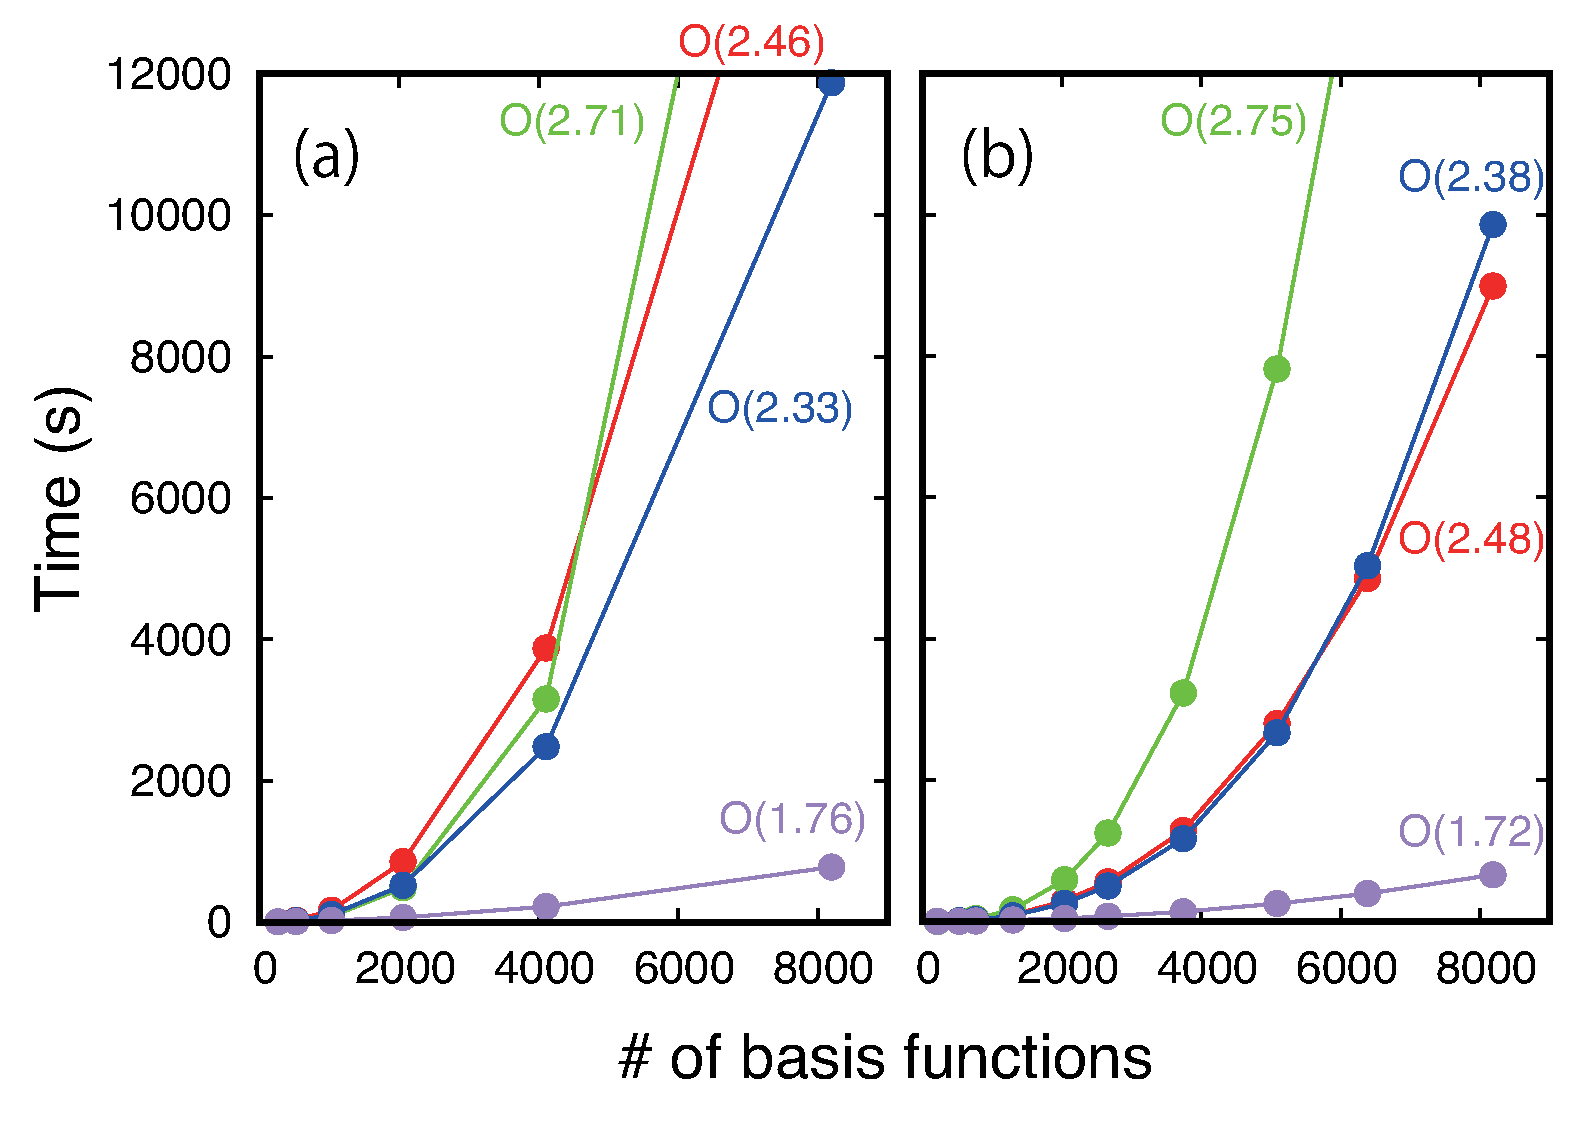
\includegraphics[width=0.525\textwidth]
{research/nakajima/ps_basis.eps}
\caption{Computational time of two-electron repulsive integrals in glucose-alanine chain (a) and H$_2$O molecular cluster (b) as a function of the number of basis functions.
The red, blue, green, and purple circles denote the analytical, GAPW, PS, and PS-GAP methods, respectively.}
\locallabel{fig:ps_basis}
\end{figure}

\begin{figure}[t]
\centering
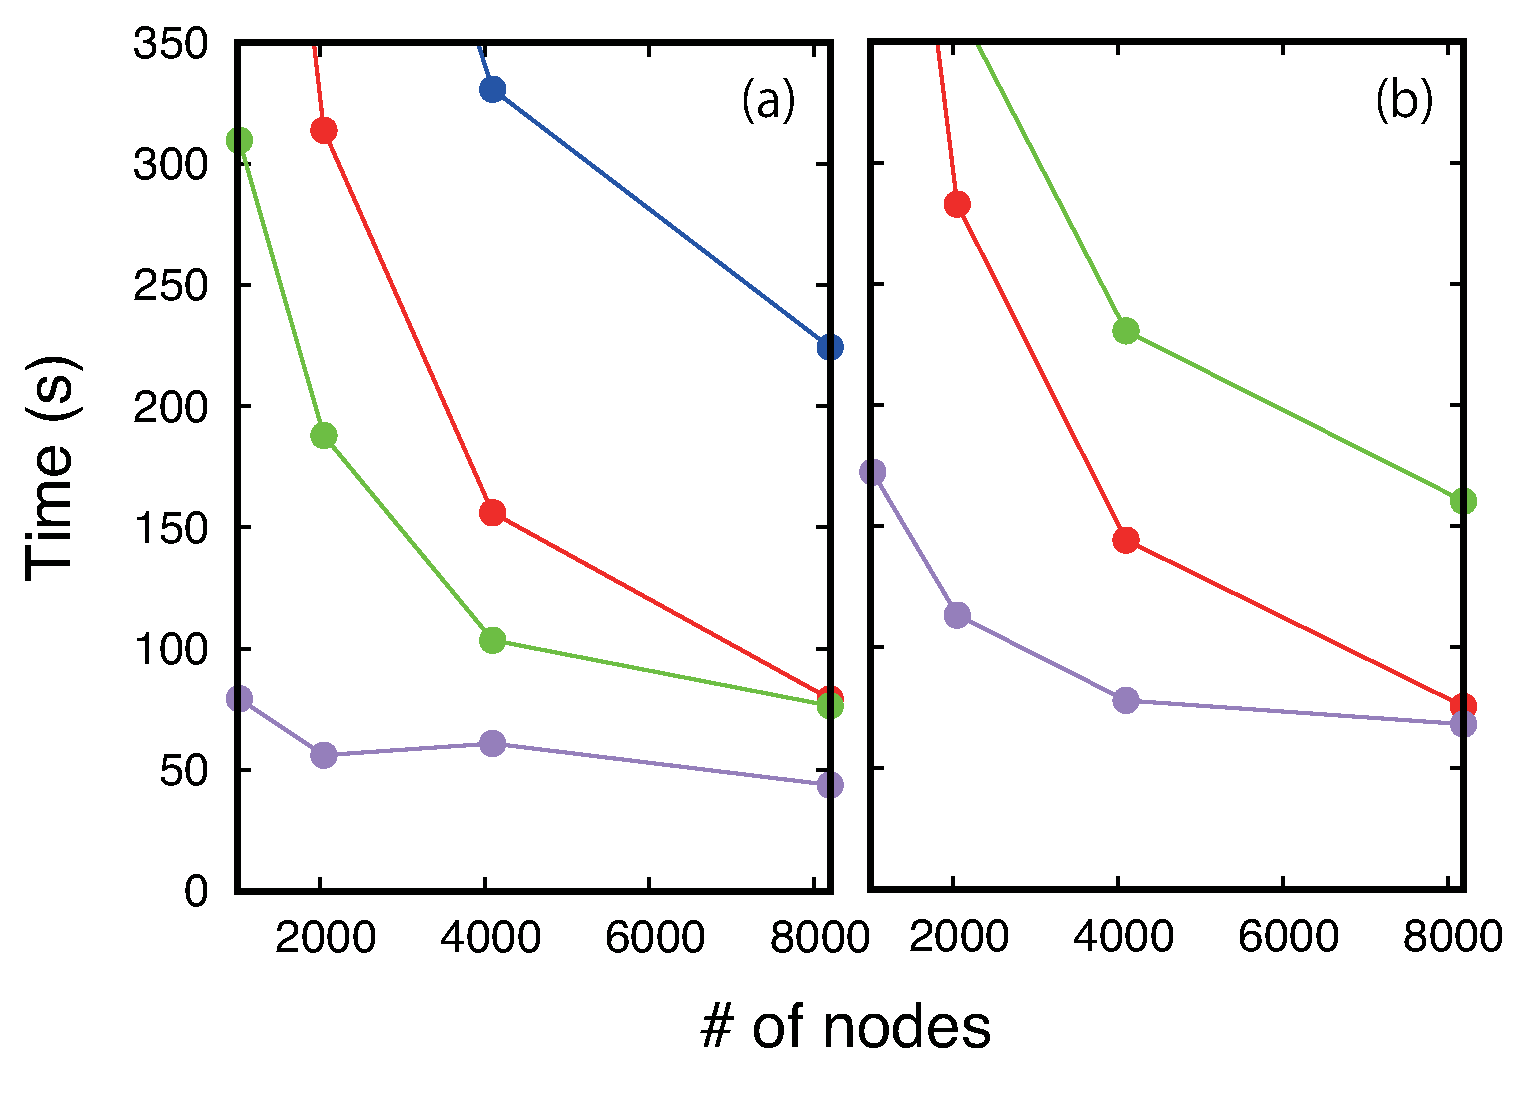
\includegraphics[width=0.525\textwidth]
{research/nakajima/ps_node.eps}
\caption{Computational time of two-electron repulsive integrals in glucose-alanine chain with 8,202 basis functions (a) and H$_2$O molecular cluster with 10,128 basis functions (b) as a function of used nodes.
The red, blue, green, and purple circles denote the analytical, GAPW, PS, and PS-GAP methods, respectively.}
\locallabel{fig:ps_node}
\end{figure}

\subsubsection{Development of massively parallel algorithm of linear response time-dependent density functional theory for excited-state calculations on peta-flops supercomputers}
Linear response time-dependent density functional theory (LR-TDDFT) is an efficient approach for the calculation for excited-states of large molecules.
In the previous study, we developed the MPI/OpenMP hybrid parallel code of LR-TDDFT calculations with random phase approximation (RPA) and Tamm–Dancoff approximation (TDA) [Int. J. Quant. Chem. 115,349 (2015).] in NTChem software.
However, the parallel scalability of this code was limited up to about 1,000 MPI processes on the K computer due to the problems of the parallelization scheme and the I/O overhead of the Davidson diagonalization in the LR-TDDFT calculations.
In this FY, we have developed a new MPI/OpenMP hybrid parallel algorithm for LR-TDDFT/RPA and LR-TDDFT/TDA calculations.
In this algorithm, we have devised an efficient parallelization scheme of the Davidson diagonalization utilizing more than 1,000 MPI processes on the peta-scale supercomputers such as the K computer.
In this scheme, the Davidson diagonalization is parallelized utilizing the distributed memory avoiding the I/O operation reading and writing data to disks.
Vectors needed for Davidson diagonalization (trial vectors, sigma vectors, and residual vectors) are divided to the two-dimensional blocks, and these blocks are distributed to each process.
Matrix-matrix and matrix-vector multiplications evaluating the residual vector and orthogonalization of trial vectors are the computation demanding tasks in the Davidson diagonalization.
These multiplications are performed efficiently applying the OpenMP parallelized basic linear algebra subprograms (BLAS) library.
The scalability of parallel algorithm has been evaluated performing some test calculations of large nano-size molecules.
The largest calculation is the calculation of crambin protein (PDB ID: 1CRN) at the LR-TDDFT/RPA/def2-SVP level (642 atoms 6,177 atomic orbitals (AOs), and 50 excited states) using from 768 to 7,680 nodes of the K computer.
The parallel scalability is good up to 4,608 nodes. Parallel speedups are 80\% and 57\% using 1,536 nodes and 4,608 nodes, respectively. 
The elapsed time is 251 minutes using 4,608 nodes, which demonstrates that the LR-TDDFT excited state calculations of molecular materials and biological molecules contacting up to 600 atoms and 6,000 AOs become routinely possible utilizing the K computer.
The new parallel LR-TDDFT code has been released with NTChem 2013 Version 7.0 on Dec. 2015.

\subsubsection{Development of analytical energy gradient for two-component relativistic time-dependent density functional theory with spin–orbit interaction}
Precise information on excited state potential energy surfaces is the most important prerequisite for a deeper understanding of photochemical reaction or the shape of absorption and luminescence spectra.
In particular, the inclusion of spin–orbit coupling and other relativistic effects is crucial for a proper description of excited-state characters, relaxation dynamics, radiative and nonradiative decay pathways, as well as lifetimes and reactivity for systems containing heavy elements.
The development and efficient implementation of an analytic gradient theory for reliable theoretical models incorporating both electron correlation and relativistic effects has been awaited.
Recently, we have developed two-component relativistic time-dependent density functional theory with spin–orbit interactions (SO-TDDFT), which is becoming popular methodologies for computing excited states containing heavy elements because of its reasonable cost and relatively high accuracy.
In this work, we have implemented the analytical gradient for two-component relativistic TDDFT with spin–orbit interactions in the NTChem program.
Our implementation is based on the derivation of the geometrical derivatives for nonrelativistic TDDFT presented by Furche and Ahlrichs.
The noncollinear exchange-correlation potential presented by Wang {\it et al}. has been applied.
The higher-order matrix elements of the noncollinear exchange-correlation kernel for the relaxed one-particle and two-particle density matrices have been derived and implemented into efficient computer codes with the aid of a newly-developed computerized symbolic algebra system.
In addition, various DFT functionals including the recently proposed range-separated hybrid functionals are applicable to the calculations of excitation energy for spin–orbit coupled states.

\subsubsection{Development of a method for electronic-structure calculations based on self-energy functional theory}
Electronic-structure calculations based on the density functional theory (DFT) have been used in quantum chemistry and providing reliable explanations and predictions of many molecular systems.
While the elaboration of techniques of DFT-based calculations is continued in the community, the limitation of the framework of DFT is known to exist and should be overcome, which is problematic particularly for strongly correlated systems.
For such systems, model Hamiltonians have been used traditionally, in which only few adjustable parameters looking important are often introduced by hand.
Among many approaches proposed so far, the approach based on the self-energy functional theory (SFT) [Potthoff, Eur. Phys. J. B 32 (2003) 429.] is promising.
It has been applied to systems with model Hamiltonians such as a Hubbard chain [Potthoff, Eur. Phys. J. B 36 (2003) 335.] and NiMnSb [Allmaier {\it et al}, Phys. Rev. B 81 (2010) 054422.],
however, no calculation based purely on SFT has not been reported to our knowledge.
Since a SFT-based calculation uses the result of exact diagonalization for the subspace appropriately chosen from the entire Hilbert space, it is expected that the many-body effects are taken into account accurately for describing the strongly correlated system.
We started to develop a method for SFT-based quantum chemistry calculations.
Specifically, we first construct the second-quantized Hamiltonian by calculating one- and two-electron integrals for a molecule and divide the entire Hilbert space into the subspaces
so that as many the molecular orbitals in the vicinity of the Fermi level are contained in one of the subspaces as computationally possible.
We then perform exact diagonalization for the subspaces and calculate the thermodynamic potential of the molecule [Potthoff, Eur. Phys. J. B 32 (2003) 429.] from the self-energies $\Sigma$ of the subspaces as $\Omega = F[\Sigma] - \mathrm{Tr} \ln (-G_0^{-1} + \Sigma)$,
where $F [\Sigma]$ is the universal functional of the self-energies and $G_0$ is the non-interacting Green's function.

\subsubsection{Theoretical study on the cooperative exciton dissociation process based on dimensional and hot charge-transfer state effects in an organic photocell}
In recent years, organic electronics devices such as electroluminescent displays, transistors, and photocells, have actively been studied because of various properties of organic materials, such as lightweight, thin film structures, flexibility, manufacturing costs, design, and so on.
We have been studying organic photocell devices.
It is critical to understand the energy conversion mechanism from the solar photon flux in organic semiconductors, especially the dynamics of strongly bound electron–hole pairs (excitons).
In organic photocells, excitons are first created by absorbing photons.
They then diffuse to the donor–acceptor interface of the organic semiconductor.
Finally, they are dissociated to create free electrons and holes after the electron (charge) transfer process.
Here, we studied the cooperative exciton dissociation process based on dimensional and hot charge transfer state effects.
In last FY, we introduced a local temperature to handle with the hot charge-transfer (CT) sate, and calculated the exciton dissociation probability based on the one-dimensional organic semiconductor model.
Although the hot CT state plays essential roles, the probabilities calculated are not enough high to efficiently separate bounded electron-hole pairs.
In this FY, therefore, we focused on the dimensional effect together with the hot CT state effect.
We showed that cooperative behaviors between both effects can significantly improve the exciton dissociation process.

\subsubsection{Development of trajectory surface hopping algorithm for the time- dependent density functional theory: Toward the understanding of working mechanisms of organic photovoltaic solar cells}
The solar cell can convert solar energy into electric energy and is a valuable resource of clean energy that is free from environment pollution.
While people have used silicon-based solar cells widely in a real life, organic photovoltaic devices are considered to be promising in a next generation due to their versatility, easy processing, low cost, and so on.
The photo-energy conversion efficiency is a critical factor in the development of new solar cells.
So it is necessary to derive a valuable relationship between the conversion efficiency and the properties of constituent organic molecules.
Nowadays, quantum chemistry calculations routinely afford (1) the energy gap between the highest occupied molecular orbital and lowest unoccupied molecular orbital, (2) excitation energies, and (3) oscillator strengths.
Although these data give guidelines to develop new photo-functional materials, they are insufficient to reveal the details of photochemical processes after light absorption;
how solar cells work relies on the mechanisms of the exciton (electron-hole pair) generation and its separation/migration.
Therefore, it is desirable to simulate the relaxation processes on the excited-state potential energy surfaces (PESs) directly and to observe the real-time behavior of electron–hole pair.
A large size of organic dye molecules hampers the on-the-fly molecular dynamics simulation by sophisticated wavefunction approaches.
Furthermore, photochemical processes involve a large number of PESs, and one must take accounts of non-adiabatic transition between these electronic states.
To satisfy these requirements, we have implemented a combined method of time-dependent density functional theory (TD-DFT) and trajectory surface hopping (TSH) algorithm.
For now, the TSH input data was taken from the TDDFT output given by the program package GAMESS.
The TSH program needs the non-adiabatic coupling vector (NACV), which is not trivial at the TDDFT level of theory.
Instead of deriving analytic NACV, we introduced isotropic scalar NAC as the overlap of wavefunctions at consecutive time steps and computed it on the fly.
Some test calculations in progress show the efficiency and robustness of the proposed method.

\subsection{Applications of original molecular theory to new materials and drugs}
\subsubsection{Theoretical study on spin-forbidden transitions of metal complexes by two-component relativistic time-dependent density functional theory}
Spin-forbidden transitions of metal polypyridyl sensitizers are studied by the two-component relativistic time-dependent density functional theory with spin–orbit interaction based on Tamm–Dancoff approximation.
The spin-forbidden transitions for a phosphine-coordinated Ru(II), DX1, as well as the modified DX1 complexes whose Ru is replaced with Fe and Os, are calculated.
The role of the central metals in spin-forbidden transitions is discussed toward the exploration for new efficient sensitizers.
In addition, we study spin-forbidden transitions of Os polypyridyl sensitizers.
The absorption spectra, including spin-forbidden-transition peaks, for the Os complexes are reasonably reproduced in comparison with the experimental ones.
The extension of the conjugated lengths in the Os complexes is investigated and found to be effective to enhance photo absorption for spin-allowed transitions as well as spin-forbidden ones.
This study provides fruitful information for a design of new dyes in terms of conjugation lengths.

\subsubsection{Large-Scale QM/MM calculations of hydrogen bonding networks for proton transfer and water inlet channels for water oxidation - Theoretical system models of the oxygen-evolving complex of photosystem II}
In order to confirm theoretical system models of photosystem II (PSII), quantum mechanics (QM)/molecular mechanics (MM) calculations using a large-scale QM model (QM Model V) have been performed to elucidate hydrogen bonding networks and proton wires for proton release pathways (PRPs) of water oxidation reaction in the oxygen-evolving complex (OEC) of PSII.
Full geometry optimizations of PRP by the QM/MM model have been carried out starting from the geometry of heavy atoms determined by the recent high-resolution X-ray diffraction (XRD) experiment on PSII refined to 1.9 \AA\ resolution.
The optimized MnMn and CaMn distances by large-scale QM/MM are consistent with the EXAFS results, removing out the discrepancy between the refined XRD and EXAFS.
Computational results from QM/MM calculations have demonstrated the labile nature of the MnaO(5)Mnd bond of the CaMn4O5 cluster in the OEC of PSII which allows left (L)-opened, quasi-central (CQ)-, and right (R)-opened structures.
This confirms the feasibility of the left- and right-hand scenarios for water oxidation in the OEC of PSII that are dependent on the hydrogen bonding networks.
The QM/MM computations have elucidated the networks structures: hydrogen bonding O. . .O(N) and O. . .H distances and O(N)H. . .O angles in PRP, together with the ClO(N) and Cl. . .H distances and O(N)H. . .Cl angles for chloride anions.
The obtained hydrogen bonding networks are fully consistent with the results from XRD and available experiments such as EXAFS, showing the reliability of our theoretical system model that is crucial for investigations of functions of PSII such as water oxidation.
The QM/MM computations have elucidated possible roles of chloride anions in OEC of PSII for proton transfers.
The QM/MM computational results have provided useful information for the understanding and explanation of several experimental results obtained with mutants of the OEC of PSII.
The possible implications of the present results are discussed in relation to our theoretical system models of PSII, strong or weak perturbations of the system structures by mutations, damage-free X-ray free-electron laser structure of PSII, and bioinspired working hypotheses for the development of artificial water oxidation systems which use 3d transition metal complexes.

\subsubsection{Full geometry optimizations of the CaMn$_4$O$_4$ model cluster for the oxygen evolving complex of photosystem II}
Full geometry optimizations of ([CaMn$_4$O$_4$(CH$_3$COO)$_8$(py)(CH$_3$COOH)$_2$], (py: pyridine) (1)) were performed at the UB3LYP theoretical level.
This model 1 is a theoretical model for the synthetic model ([CaMn$_4$O$_4$(ButCOO)$_8$(py)(ButCOOH)$_2$], (But: t-butyl) (2)) which closely mimics the native oxygen evolving complex (OEC) in photosystem II.
It was shown that the X-ray structure of 2 was well reproduced by 1 in the (Mn1(III), Mn2(IV), Mn3(IV), Mn4(III)) valence state with the unprotonated O5 (O5 = O2-), and two different valence states were obtained in the one-electron oxidized state.
Importance of the Jahn-Teller effect of the Mn(III) site for the structural deformations was presented.

\subsubsection{Theoretical study on selective recognition of biomolecule in supramolecule}
The purpose of this study is to analyze and understand of molecular recognition using quantum chemical calculations.
In 2009, Sawada {\it et al}. observed only single nucleotide duplex could form stably in water inside artificial cage-like supramolecule [Sawada {\it et al}. Nature Chemistry 1, 53 (2009).].
Since it was said that at least four complementary nucleotide base pairs had been necessary in order to form stable structure in water, this result can be called great progress.
In our study, we approached this issue in terms of the molecular orbital (MO) method and tried to clarify structural stability and selectivity mechanism of the target.
The selectivity in this target is that single base pair is spontaneously formed as anti-Hoogsteen (AH) type, not Watson–Click (WC) type.
In order to elucidate this selectivity, we prepared both AH-type and WC-type nucleotide duplex and performed structure optimizations with/without surrounding cage-like supramolecule.
According to the result, AH-type structure is more stable than WC-type one by 53.1 kcal/mol inside cage-like supramolecule and the same energy gain becomes only 0.2 kcal/mol without the supramolecule.
Moreover, our calculation indicates the importance of non-covalent bonding between the cage and nucleotide duplex which originates from $\pi$-$\pi$/CH-$\pi$ interaction.

\section{Schedule and Future Plan}
In the next financial year, we will continue to develop new algorithms and improve the parallel efficiency of the NTChem2013 suit of program.
In the present implementation of LR-TDDFT, the replicated memory algorithm is adopted for the evaluations of Fock like matrix.
This situation limits the application of the present code to the systems having less than 7,000 AOs on the K computer.
To overcome this problem, we are developing the distributed-memory parallel code of Fock-like matrix calculations.
Furthermore, the spin–orbit coupling often plays an important role for the excites states containing heavy elements.
We are developing the massively parallel algorithm and code of two-component relativistic LR-TDDFT to account for the spin–orbit interactions explicitly in the excited state calculations.
We will also develop transition properties and nonadiabatic coupling constant matrix elements, which are the key quantity in the description of excited-state dynamics.
In addition, for further acceleration of the PS and PS-GAP methods, we are planning to do coding and tuning of related programs in NTChem so that we will apply the improved PS and PS-GAP methods to several large molecular systems.
For self-energy functional theory (SFT), we further will continue to parallelize the calculations of one- and two-electron integrals and of exact diagonalization and of Green's functions.
The implementation of SFT-based electronic-structure calculations for periodic systems are in progress.
It is interesting to develop a unified approach to the understanding of the internal conversion (IC) and intersystem crossing (ISC) processes.
The suppression of unfavorable quenching pathways may help the design of new organic materials with high efficiencies.
One of the attractive points in NTChem program is the availability of relativistic methods.
The spin–orbit TDDFT (SO-TDDFT), in particular, can deal with both singlet and triplet states on an equal footing.
The SO-TDDFT/TSH simulation involving both spin states can be performed in a similar way as the singlet-state-only TSH because a natural extension of the conventional TDDFT coupling yields the SO-TDDFT counterpart.
Another direction is to develop a hybrid method of quantum mechanics/molecular mechanics (QM/MM).
Bulk heterojunction solar cell, for example, is a composite system of p- and n-type layers.
It is natural to split the whole system to reduce the computational cost.
The QM method is applied to the small region, the interface between the p- and n-type materials, while the remaining part is treated as MM.
The method will give insights into the environmental effects on charge transport dynamics that occurs at the interface.
We earnestly hope that NTChem will be an important tool leading the way toward a new frontier of computational molecular science.


%%% DO NOT EDIT BELOW

\section{Publications}

%\printbibliography[keyword=journal, heading=subbibliography, title={Journal Articles}, prefixnumbers={1-}, resetnumbers=true]
%\printbibliography[keyword=proceedings, heading=subbibliography, title={Conference Papers}, prefixnumbers={2-}, resetnumbers=true]
%\printbibliography[keyword=invited, heading=subbibliography, title={Invited Talks}, prefixnumbers={3-}, resetnumbers=true]
%\printbibliography[keyword=poster, heading=subbibliography, title={Posters and Presentations}, prefixnumbers={4-}, resetnumbers=true]
%\printbibliography[keyword=deliverable, heading=subbibliography, title={Patents and Deliverables}, prefixnumbers={5-}, resetnumbers=true]

\printbibliography[keyword=journal, heading=subbibliography, title={Journal Articles}, resetnumbers=true]
\printbibliography[keyword=proceedings, heading=subbibliography, title={Conference Papers}]
\printbibliography[keyword=invited, heading=subbibliography, title={Invited Talks}]
\printbibliography[keyword=poster, heading=subbibliography, title={Posters and Presentations}]
\printbibliography[keyword=deliverable, heading=subbibliography, title={Patents and Deliverables}]

\end{refsection}

\begin{refsection}[research/yunoki/group.bib]
\nocite{*}
\chapter{Computational Materials Science Research Team}

\section{Members}

\begin{itemize}
  \item[] Ichiro Kobe (Team Leader)
  \item[] Jiro Kobe (Senior Scientist)
  \item[] Saburo Kobe (Research Scientist)
\end{itemize}

\section{Research Activities}

Text for research activities.

\section{Research Results and Achievements}

Text for research Results and achievements. Journal-artcile~\cite{sample-journal}.
Conference-paper~\cite{sample-conference}.
Invited-talk~\cite{sample-invited}.

For cross referencing, use \verb|\locallabel| and \verb|\localref| to avoid conflicting names defined by other groups. For example, a figure can be referenced as Figure~\localref{fig:sample-label1}.

\begin{figure}
\centering
  
\includegraphics[width=0.5\textwidth,keepaspectratio,natwidth=193,natheight=40]
  {sample_division/sample_group/test1.png}
  \caption{Caption for a sample figure}
  \locallabel{fig:sample-label1}
\end{figure}

\section{Schedule and Future Plan}

Text for schedule and future plan.

%%% DO NOT EDIT BELOW

\section{Publications}

%\printbibliography[keyword=journal, heading=subbibliography, title={Journal Articles}, prefixnumbers={1-}, resetnumbers=true]
%\printbibliography[keyword=proceedings, heading=subbibliography, title={Conference Papers}, prefixnumbers={2-}, resetnumbers=true]
%\printbibliography[keyword=invited, heading=subbibliography, title={Invited Talks}, prefixnumbers={3-}, resetnumbers=true]
%\printbibliography[keyword=poster, heading=subbibliography, title={Posters and Presentations}, prefixnumbers={4-}, resetnumbers=true]
%\printbibliography[keyword=deliverable, heading=subbibliography, title={Patents and Deliverables}, prefixnumbers={5-}, resetnumbers=true]

\printbibliography[keyword=journal, heading=subbibliography, title={Journal Articles}, resetnumbers=true]
\printbibliography[keyword=proceedings, heading=subbibliography, title={Conference Papers}]
\printbibliography[keyword=invited, heading=subbibliography, title={Invited Talks}]
\printbibliography[keyword=poster, heading=subbibliography, title={Posters and Presentations}]
\printbibliography[keyword=deliverable, heading=subbibliography, title={Patents and Deliverables}]

\end{refsection}

\begin{refsection}[research/sugita/group.bib]
\nocite{*}
\chapter{Computational Biophysics Research Team}

\section{Members}

\begin{itemize}
 \item[] Yuji Sugita (Team Leader (Concurrent))*, **
 \item[] Osamu Miyashita (Senior Research Scientist)
 \item[] Jaewoon Jung (Research Scientist)
 \item[] Chigusa Kobayashi (Research Scientist)
 \item[] Yasuhiro Matsunaga (Research Scientist)
 \item[] Hiromi Kano (Assistant)
 \item[] Takaharu Mori (Research Scientist (Concurrent))**
 \item[] Isseki Yu (Research Scientist (Concurrent))**
 \item[] Raimondas Galvelis (Postdoctoral Researcher (Concurrent))**
 \item[] Takao Yoda (Visiting Scientist) ***
 \item[] Mitsunori Ikeguchi (Visiting Scientist)****
 \item[] Naoyuki Miyashita (Visiting Scientist)
 \item[] Michael Feig (Visiting Scientist)
\end{itemize}

* The main affiliation of these people is Laboratory for Biomolecular Function Simulation, Computational Biology Research Core, RIKEN Quantitative Biology Center.

** The main affiliation is RIKEN Theoretical Molecular Science Laboratory.

*** The main affiliation is Nagahama Bio Institute.

**** The main affiliation is Yokohama City University.

\section{Research Activities}

In this team, we have developed GENESIS(Generalized Ensemble Simulation
System) for molecular dynamics simulations. The key features of GENESIS
are that it is highly parallelized for K and other massively parallel
supercomputers and that GENESIS contains a lot of enhanced
conformational sampling methods and various molecular models for
multi-scale and multi-resolution simulations. We have already open the
code of GENESIS as free software under the license of GPLv2 and will
update it every two year by adding new functions and optimizing the code
into K or other computational platforms. These activities are necessary,
in particular, for biological applications, since many interesting
biological phenomena happen on the milliseconds or slower but current
all-atom MD simulations cover only 1-10 microseconds on the
general-purpose supercomputers or GPU clusters. We intend to spread
GENESIS into academia as well as industries as a basic MD program that
is useful for research and development. 

\section{Research Results and Achievements}

\subsection{Developement of GENESIS}

We have already optimized GENESIS for large scale MD simulations on K
computer. In the given fiscal year, we further optimized it by
increasing parallel efficiency and enlarging the available number of
processors. First, we make use of a multiple-program, multiple-data
approach by separating computational resources responsible for real
space and reciprocal space interactions. Second, we assign multiple time
step integrator where time-consuming parts are skipped regularly based
on the multiple-program and multiple-data approach. Our new
implementation was tested on the K computer, and we could obtain very
good performance results for big systems consisting of 1 million, 8.5
million, and 28 million atoms systems just increasing the parallel
efficiencies. One MD cycle with the PME calculations for systems
containing 1 million, 8.5 million, and 28 million atoms could be
finished within 2.8 ms, 5.4 ms, and 8 ms (Figure~\localref{fig:fig01}).

\begin{figure}[tbp]
\centering
  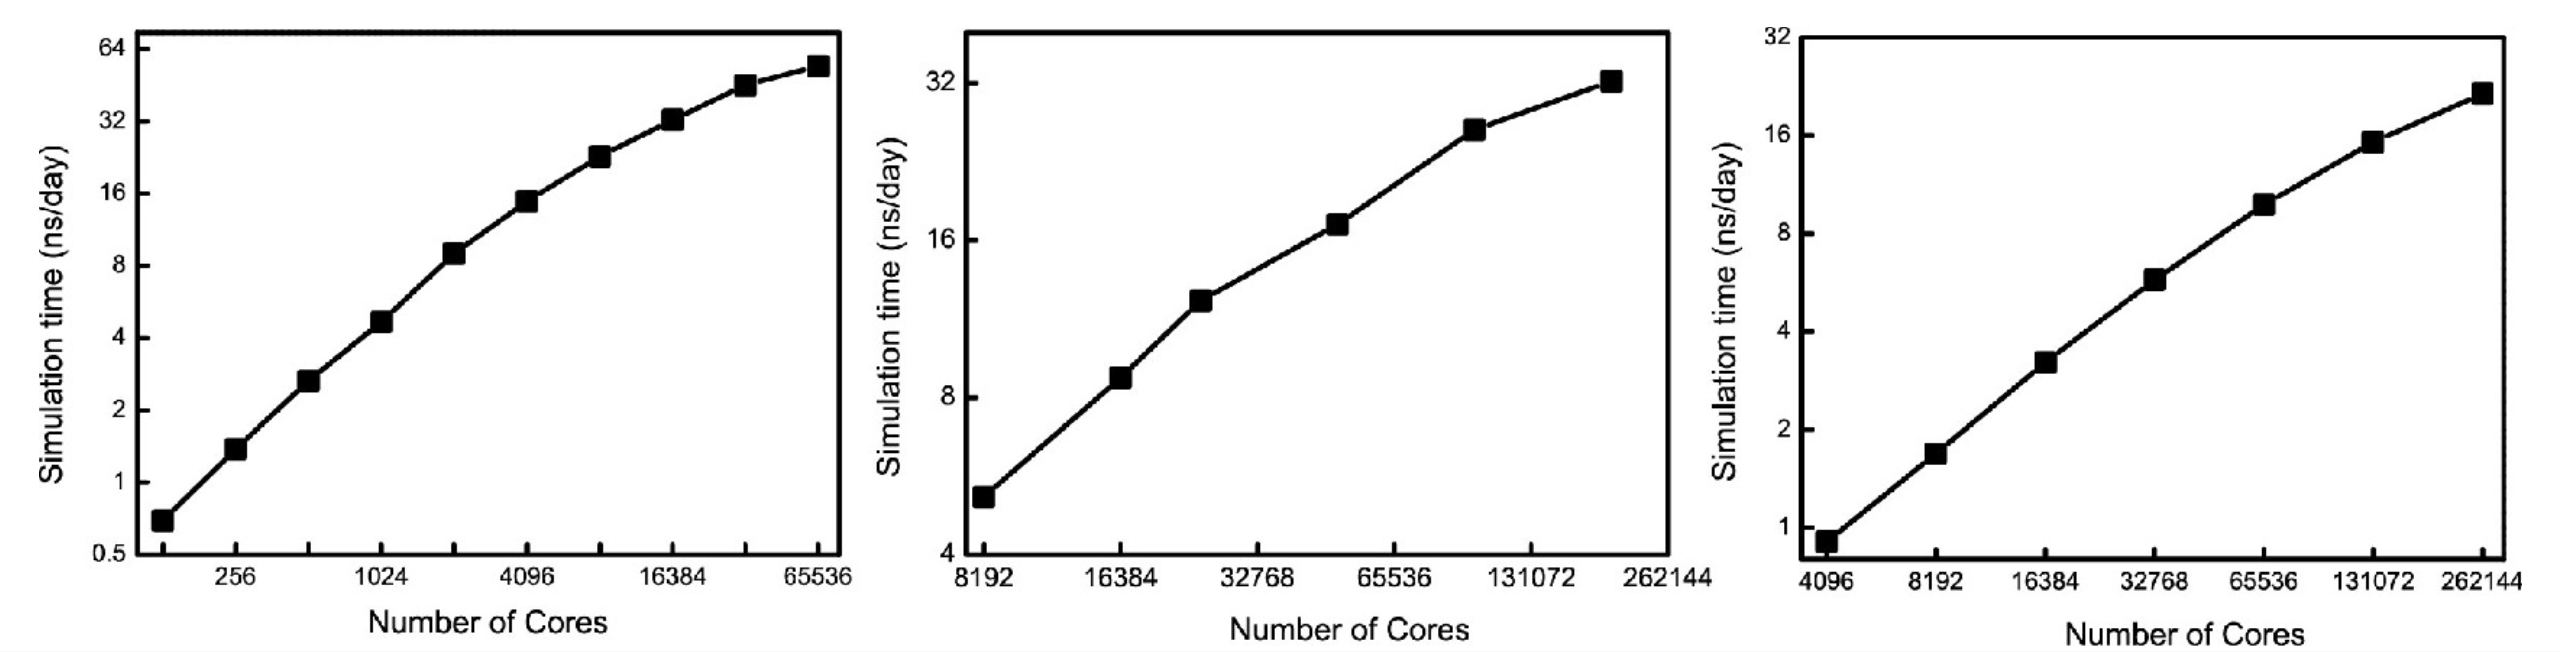
\includegraphics[width=0.8\textwidth,keepaspectratio,natwidth=193,natheight=40]
  {research/sugita/fig01.png}
  \caption{GENESIS performance of 1M (left), 8.5M (middle), and 28M (right) systems}
  \locallabel{fig:fig01}
\end{figure}

\subsection{Multi-resolution simulation methods for reactions couple with large conformational changes}

Recently, experimental studies proposed that large conformational
changes of proteins play important roles on biological functions. The
conformational changes can originate as domain motions, where rigid
structural units (domains) change their positions and/or orientations
with respect to each other through flexible hinges or loops. It is
difficult to investigate atomistic details of multi-domain proteins by
experimental studies. In addition, it is still difficult to simulate
using all-atom MD due to the slow time-scale. To overcome the
difficulties, we have developed multi-resolution simulation method
including the following three steps; 1. Analysis for “dynamic domains”
and the magnitude of local domain motions in a protein through “Motion
Tree”, a tree diagram that describes conformational changes in a
hierarchical manner from two structures. (Koike et al., {\it J. Mol. Biol.},
2014) 2. Development of a structure-based coarse-grained (CG) model
enables a stable and efficient MD simulation from the information of
domain motion obtained by ``Motion Tree''~\cite{Kobayashi01}. The CG
model provides a stable trajectory that is comparable to experimental
studies and long-time all-atom MD simulations. 3. Performing sampling
simulations with the CG model and investigate conformational changes in
response to reactions in biological systems. We examine how many CVs are
required to capture the correct transition-state structure during the
open-to-close motion of adenylate kinase using a coarse-grained model in
the mean forces string method to search the minimum free-energy
pathway~\cite{Kobayashi02}.

\subsection{Systematic evaluation of collective variable choice for describing conformational changes of a protein}

Collective variables (CVs) are often used in molecular dynamics
simulations based on enhanced sampling algorithms to investigate large
conformational changes of a protein. The choice of CVs in these
simulations is essential because it affects simulation results, and
impacts on the free-energy profile, the minimum free-energy pathway
(MFEP), and the transition-state structure. Here, we examine how many
CVs are required to capture the correct transition-state structure
during the open-to-close motion of Adenylate Kinase using a
coarse-grained model in the mean forces string method to search the
MFEP. Various numbers of large amplitude principal components (PCs) are
tested as CVs in the simulations. The incorporation of local coordinates
into CVs, which is possible in higher dimensional CV spaces, is
important for capturing a reliable MFEP. The Bayesian measure proposed
by Best and Hummer is sensitive to the choice of CVs, showing sharp
peaks when the transition-state structure is captured. We thus evaluate
the required number of CVs needed in enhanced sampling simulations for
describing protein conformational changes (Figure~\localref{fig:fig02}~\cite{Matsunaga02}).

\begin{figure}[tbp]
\centering
  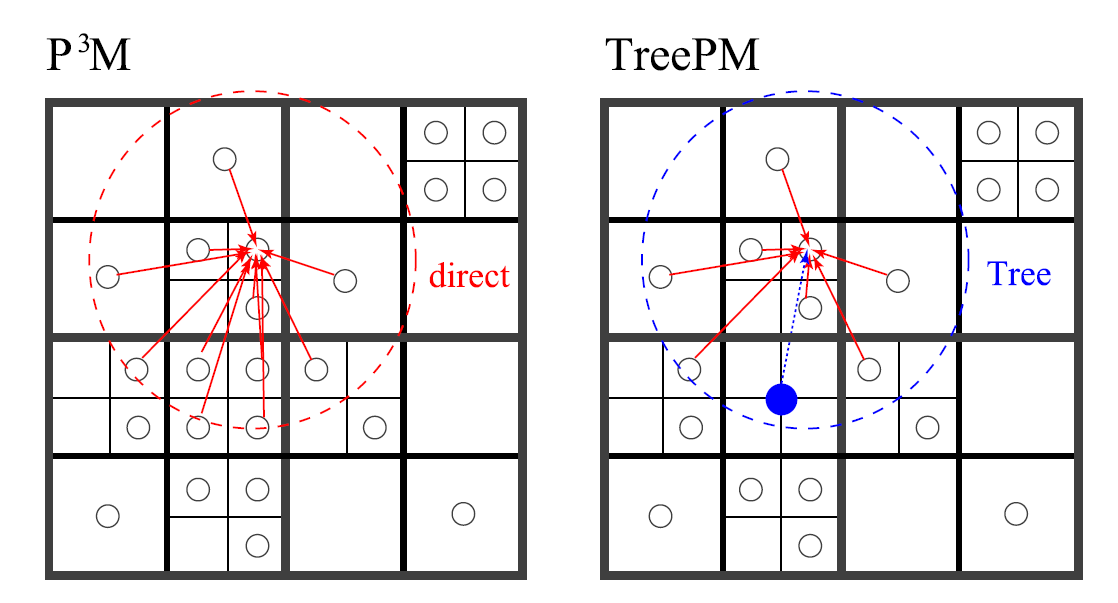
\includegraphics[width=0.8\textwidth,keepaspectratio,natwidth=193,natheight=40]
  {research/sugita/fig02.png}
  \caption{Free-energy landscape in the distances between domains'
 centers of mass. Lines indicate minimum free energy paths calculated in
 2D (dark blue), 3D (light blue), 10D (yellow), and 20D (red) principal
 component spaces.} 
  \locallabel{fig:fig02}
\end{figure}

\subsection{Molecular crowding effect on GTP hydrolysis reaction in Ras-GAP complex}

Macromolecular crowding effects have essential role in biomolecular
system. Such effects have been extensively investigated experimentally,
and also in classical Molecular Dynamics (MD) calculations. However, in
the quantum chemistry level, those effects are not investigated due to
the computational costs and methodological difficulties. In this study,
we studied the molecular crowding effect on the GTP hydrolysis reaction
in Ras-GAP complex by QM/MM RWFE method, which can take crowding effects
into account with a reasonable computational cost. We modeled a crowding
environment by adding 7 BSAs to the system as a crowder, and refined the
reactant and transition states of the hydrolysis reaction by QM/MM RWFE
method, where MD calculations were performed by GENESIS at
K-computer. The structural difference around GTP were not significant
between solution and crowding environment. However, there was a large
difference in the electrostatic potential (ESP) imposed by the
surroundings as shown in Figure~\localref{fig:fig03}. This large ESP
change suggests that there must be significant differences in the free
energy barrier between crowding and solution environments.

\begin{figure}[tbp]
\centering
  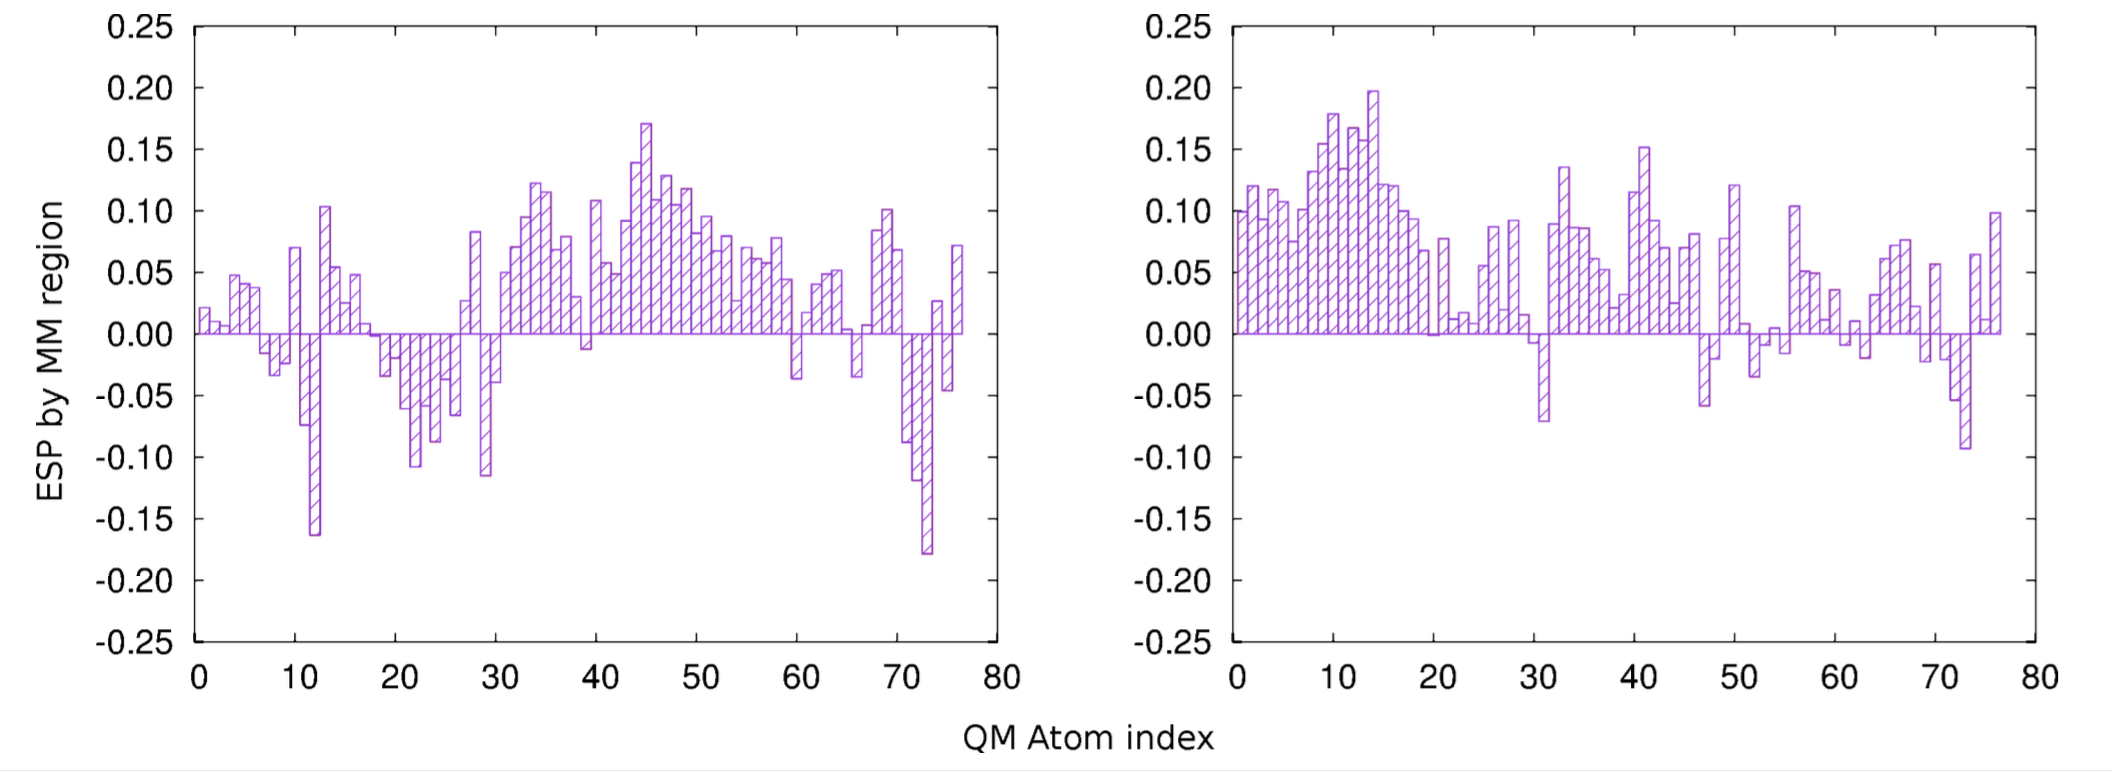
\includegraphics[width=0.8\textwidth,keepaspectratio,natwidth=193,natheight=40]
  {research/sugita/fig03.png}
  \caption{Electrostatic potential on QM atoms of the reactant state in
 the model crowding environment (left) and solution (right). QM atom
 index 43-55 corresponds to triphosphate moiety of GTP.} 
  \locallabel{fig:fig03}
\end{figure}

\section{Schedule and Future Plan}

So far, GENESIS has been optimized mainly on K computer. In this year or
later, we consider other platforms than K, such as intel CPU cluster,
nvidia GPU processor, and post K. Since these CPU (or GPU) architectures
are quite different with each other, a single MD kernel does not work
well for all the different computational platforms. So, GENESIS will
have multiple kernels that are optimized to one of the computational
platforms. The disadvantage of this approach is that we have more effort
on programming, reducing potential bugs for each kernel, and so on. It
should be hard task for our team, but there is no other good ways to
improve the performance of GENESIS in multiple platforms. 

We would like to simulate more and more large biological systems for
investigating slow biological dynamics. For this purpose, we need to
develop multi-scale and multi-resolution programs that are scalable on K
or post-K computers. Currently, GENESIS/SPDYN is useful for all-atom MD
simulations on these supercomputers, but does not show good performance
on CG-modeling and simulations of biological systems due to the small
number of particles and load-balance problems. We need a new program
that is suitable for such CG-modeling and simulations by introducing a
different parallelization scheme. Such new program, which we call CGDYN,
will be developed soon. 

Another important aspect is the introduction of quantum effect to
investigate the chemical reactions in enzymes. Bond-formation or
breaking can not be simulated by using classical force fields, but
should be investigated by using ab initio Quantum theory. Considering
the large system size in biological systems, only possible approach is
to use QM/MM hybrid calculations. We have a basic QM/MM code for
computing potential energies of QM/MM systems and optimizing the systems
based on the hybrid QM/MM potential energy functions. We plan to extend
the calculations for larger periodic boundary systems and to allow the
reaction calculations in proteins. 

%%% DO NOT EDIT BELOW

\section{Publications}

%\printbibliography[keyword=journal, heading=subbibliography, title={Journal Articles}, prefixnumbers={1-}, resetnumbers=true]
%\printbibliography[keyword=proceedings, heading=subbibliography, title={Conference Papers}, prefixnumbers={2-}, resetnumbers=true]
%\printbibliography[keyword=invited, heading=subbibliography, title={Invited Talks}, prefixnumbers={3-}, resetnumbers=true]
%\printbibliography[keyword=poster, heading=subbibliography, title={Posters and Presentations}, prefixnumbers={4-}, resetnumbers=true]
%\printbibliography[keyword=deliverable, heading=subbibliography, title={Patents and Deliverables}, prefixnumbers={5-}, resetnumbers=true]

\printbibliography[keyword=journal, heading=subbibliography, title={Journal Articles}, resetnumbers=true]
\printbibliography[keyword=proceedings, heading=subbibliography, title={Conference Papers}]
\printbibliography[keyword=invited, heading=subbibliography, title={Invited Talks}]
\printbibliography[keyword=poster, heading=subbibliography, title={Posters and Presentations}]
\printbibliography[keyword=deliverable, heading=subbibliography, title={Patents and Deliverables}]

\end{refsection}

\begin{refsection}[research/makino/group.bib]
\nocite{*}
\chapter{Particle Simulator Research Team}

\section{Members}

\begin{itemize}
  \item[] Junichiro Makino (Team Leader)
  \item[] Keigo Nitadori (Research Scientist)
  \item[] Yutaka Maruyama (Research Scientist)
  \item[] Masaki Iwasawa (Postdoctoral Researcher) 
  \item[] Ataru Tanikawa (Postdoctoral Researcher)
  \item[] Takayuki Muranushi (Postdoctoral Researcher)
  \item[] Natsuki Hosono (Postdoctoral Researcher)
  \item[] Daisuke Namekata (Postdoctoral Researcher)
  \item[] Miyuki Tsubouchi (Technical Staff)

\end{itemize}

\section{Research Activities}

We are developing particle-based simulation software that can be used
to solve problems of vastly different scales.

Simulation schemes for hydrodynamics and structural analysis can
bedivided into grid-based and particle-based methods. In grid-based methods, the computational region is mapped to
regular or irregular grids. Continuous distributions of physical
values are represented by discrete values at grid points, and the
governing partial differential equation is approximated to a set of
finite difference equations.

\begin{figure}[tbp]
\centering
  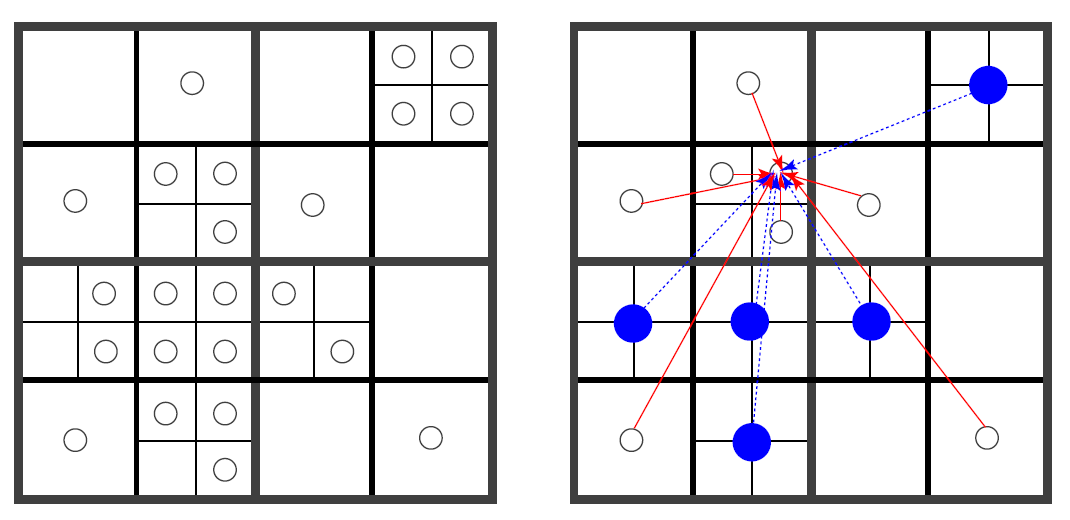
\includegraphics[width=0.8\textwidth,keepaspectratio]
  {research/makino/fig01.png}
  \caption{Basic idea of tree algorithm}
  \locallabel{fig:fig01}
\end{figure}


%% \begin{figure}[tbp]
%% \centering
%%   \includegraphics[width=0.8\textwidth,keepaspectratio]
%%   {research/makino/fig02.png}
%%   \caption{XXX}
%%   \locallabel{fig:fig02}
%% \end{figure}

%% \begin{figure}[tbp]
%% \centering
%%   \includegraphics[width=0.8\textwidth,keepaspectratio]
%%   {research/makino/fig03.png}
%%   \caption{XXX}
%%   \locallabel{fig:fig03}
%% \end{figure}

In the case of the particle-based methods, physical values are
assigned to particles, while the partial differential equation is
approximated by the interactions between particles. 

Both methods are widely used, and they have their advantages and
disadvantages. The computational cost of grid-based schemes is
generally lower than that of particle-based methods with similar
number of freedoms. Thus, if an near-uniform grid structure is
appropriate for the problem to be solved, grid-based methods perform
better. 

The advantage of the particle-based methods comes from the fact that
they use "Lagrangian" schemes, in which the particles move following
the motion of the fluid in the case of the CFD calculation. In the
case of grid-based methods, we generally use "Eulerian" schemes, in
which the grid points do not move. 

There are three points in which the Lagrangian schemes are better than
Eulerian schemes.  One is that the Lagrangian schemes are, to some
extent, adaptive to the requirement of the accuracy, since when a
low-density region is compressed to become high density, Second one is
that the timestep criteria are quite different. In the case of the
Lagrangian schemes, the timestep is determined basically by local
sound velocity, while in the Eulerian scheme by global velocity. Thus,
if a relatively cold fluid is moving very fast, the timestep for the
Eulerian schemes can be many orders of magnitude shorter than that for
Lagrangian schemes. Finally, in the case of fast-moving
low-temperature fluid, the required accuracy would be very high for
Eulerian scheme, since the error comes from the high velocity, while
that error would be transferred to internal energy of the fluid
element which is much smaller than that of the kinetic motion.

Of course, there are disadvantages of Lagrangian schemes. The primary
one is the difficulty of construction of such schemes in two or higher
dimensions.  In the case of one-dimensional calculation, it is easy to
move grid points following the motion of the fluid, but in two or
higher dimensions, the grid structure would severely deform if we let
the grid points follow the flow. Thus, we have to reconstruct the grid
structure every so often. This requirement causes the program to
become complex. Moreover, reconstruction of the grid structure (so
called remeshing) means we lose numerical accuracy.

Particle-based methods "solve" this difficulty by not requiring any
mesh. In particle-based methods, particles interact with its
neighboring particles, not through some connection through grid, but
through distance-dependent kernel functions. Thus, there is no need of
remeshing. As a result, particle-based schemes are simple to
implement, and can give reasonable results even when the deformation
is very large. Another important advantage is that it is relatively
easy to achieve high efficiency with large-scale particle-based
simulation.

In the case of grid-based schemes, in order achieve some adaptivity to
the solution, we have to use either irregular grid or regular grid
with adaptive mesh refinment. In both cases, adaptivity breaks the
regularity of the mesh structure, resulting in non-contiguous access
to the main memory. In the case of the particle-based schemes, it does
require some irregular memory access, but it is relatively
straightforward to make good use of spacial locality, and thereby
achieving high efficiency. Similarly, very high parallel performance
can be achieved.

However, it has its own problems. In the case of the SPH method, it
has been known that the standard scheme cannot handle the contact
discontinuity well. It also require rather strong artificial
viscosity, which results in very low effective Reynolds number.

Thus, in many fields of computational sciences, many groups are
working on implementation of high-performance particle-based
simulation codes for their specific problem.

One serious problem here is that, high-performance, highly-parallel
simulation codes for particle-based simulations are becoming more and
more complex, in order to make full use of modern supercomputers. We
need to distribute particles to many computing nodes in an appropriate
way, so that the communication between nodes is minimized and at the
same time near-optimal load balance is achieved. Within each nodes, we
need to write an efficient code to find neighbor particles, rearrange
data structure so that we can make good use of the locality, make good
use of multiple cores and SIMD units within each core.

Even for the case of very simple particle-particle interaction such as the Lenard-Jones potential or Coulomb potential, the calculation code tends to be very large, and since the large fraction of the code is written to achieve a high efficiency on a specific architecture, it becomes very hard to port a code which is highly optimized to one architecture to another architecture.

Our goal is to develop a "universal" software that can be applied to a variety of problems whose scales are vastly different.  
In designing such universal software, it is important to ensure that it runs efficiently on highly parallel computers such as the K computer. Achieving a good load balance with particle-based simulation is a difficult task, since using a regular spatial decomposition method causes severe load imbalance, though this works well for grid-based software. Consequently, we have developed an adaptive decomposition method that is designed to work in a way that the calculation time on each node is almost the same, resulting in near-optimal load balance.

The strategy to develop such a universal software is as follows.

We first construct an highly parallel and very efficient implementation of the TreePM algorithm for  gravitational N-body problem. This is actually not a completely new implementation, but the GreeM code developed by researchers of the Strategic Program for Innovative Research (SPIRE) Field 5 “The origin of matter and the universe. In collaboration with the Field 5 researchers, we improve the
efficiency of the code and study the issues of  the data structure, domain decomposition, load balance strategy etc.

In the second stage, we will develop a prototype of the parallel particle simulation platform. We will design the platform so that it can be used for multiple physical systems. In practice, we consider the following three applications as the initial targets.

1. Gravitational N-body simulation
2. Smoothed Particle Hydrodynamics 
3. Molecular Dynamics

In the meantime, we will also investigate the way to improve the performance and accuracy of the current particle-based algorithms for hydrodynamics.

\section{Research Results and Achievements}

As we stated in section 2, we are working on the three major subtopics, in order to develop the universal platform for particle simulations.

In the following, we briefly describe the status of our research in each subtopic.

\subsection{High-performance gravitational N-body solver.}

We use the TreePM algorithm as the basic method for the evaluation of
gravitational interaction between particles. TreePM is a combination
of the tree method and the $\rm P^3M$ (particle-particle
particle-mesh) scheme. Figure  \localref{fig:fig01} shows the basic idea of the tree
algorithm. The space is divided into a hierarchical octree structure
(quadtree in the figure). Division is stopped when a cell contains one
or no particle. When we calculate the force on a particle, we evaluate
the force from a group of particles, with size larger for more distant
particles. In this way, we can reduce the calculation cost from O(N2)
to O(N log N).


The tree algorithm is widely used, but when the periodic boundary
condition is applied, we can actually use a more efficient efficient
scheme, since we can calculate the long-range, periodic term using
FFT. The $\rm P^3M$ scheme has been used for such problem, but it has
the serious problem that when the density contrast becomes high, the
calculation cost increases very quickly. The TreePM scheme solves this
difficulty by using the tree algorithm to evaluate the forces from
nearby particles. Even when there are very large number of neighbor
particles, the calculation cost does not increase much, since the
calculation cost of the neighbor force is proportional to the
logarithm of the number of neighbors.



In order to map the problem to the distributed-memory parallel
computer such as the K computer, we adopted the approach to divide the
space into domains and assign particles in one domain to one
calculation node. We used the orthogonal recursive multisection method
developed by the team leader some years ago. It is the generalization
of the orthogonal recursive bisection (ORB), which has been widely
used in many parallel implementations of the tree algorithm.

With ORB, we recursively divide space into two halves, each with the
same number of particles. An obvious disadvantage of the ORB approach
is that it can utilize the computing nodes of integral powers of
two. Thus, in the worst case we can use only half of the available
nodes.

The difference between the multisection method and the ORB is that
with the multisection method we allow the divisions to arbitrary
number of domains, instead of bisection. This would allow too many
possible divisions. In our current implementation, we limit the number
of levels to three, and make the numbers of divisions at all levels as
close as possible. Thus, our domain decomposition is topologically a
simple three-dimension grid. This fact makes the multisection method
well suited to the machines with the 3D torus network like the K
computer.



We have developed a "reference code" for gravitational N-body
simulation on the K computer. This code is fairly well optimized for
the K computer, and shows quite good scalability for even for
relatively small-size problems. The asymptotic speed per timestep for
large number of nodes is around 7ms. This speed is comparable to that
of highly optimized molecular dynamics codes on K, even though our
code is designed to handle highly inhomogenous systems.

We used this code as the reference implementation for more generalized
particle simulation platform which will be described in the next
subsection.

\subsection{Particle Simulation Platform.}

In FY 2014, We have completed and released Version 1.0 of the particle
simulation platform, which we call FDPS (Framework for Developing
Particle Simulator). In FY 2015, we have applied a number of
improvements to FDPS. 

The basic idea of FDPS is that the application developer (or the user)
specified the way the particles interact with each other, and the rest
is taken care by FDPS. Here, "the rest" includes domain decomposition
and re-distribution of particles, evaluation of interactions between
particles, including those in different domains (different MPI
processes, for example).

In practice, there are many additional details the user should
give. Consider a relatively simple case of particles interacting with
softened 1/r potential. There are a number of small but important
points one has to decide on. For example, what algorithm should be
used for the interaction calculation? Even if we limit the
possibilities to reasonably adaptive schemes for open boundary
problems, we have the choice between Barnes-Hut tree and FMM. For both
algorithms, there are many different ways to parallelize them on
distributed-memory parallel computers. Also, there are infinitely many
variations for the time integration schemes.

The base layer of FDPS offers the domain decomposition based on the
recursive multisection algorithm, with arbitrary weighting function
for the load balancing. It also offers the parallel implementation of
interaction calculation between particles.

The domain decomposition part takes the array of particles on each
node as the main argument. It then generates an appropriate domain for
each node, redistribute particles according to their locations, and
returns.

The interaction calculation part takes the array of particles, the
domain decomposition structure, and the specification of the
interaction between particles as main arguments. The actual
implementation of this part need to take into account a number of
details. For example, the interaction can be of long-range nature,
such as gravity, Coulomb force, and interaction between computational
elements in the boundary element method (BEM). In this case, the user
should also provide the way to construct approximations such as the
multipole expansion and the way to estimate error. The interaction
might be of short-range nature, with either particle-dependent or
independent cutoff length. In these cases, the interaction calculation
part should be reasonably efficient in finding neighbor particles.

We have successfully implemented all of these functionalities in FDPS
version 1.0. (\url{https://github.com/FDPS/FDPS}). Using FDPS, a
gravitational N-body simulation code can be written in 120 lines, and
that code is actually fully scalable even to full-node runs on K
computer. For SPH calculations, we have also achieved similar scaling.

FDPS is implemented as a class template library in C++ language. It
receives the class definition of particles and a function (or multiple
functions in the case of complex interactions) to evaluate the
interaction between particles. When a user program is compiled with
the FDPS library, the class template is instantiated with the
user-specified definition of the particle class. Thus, even though the
FDPS library functions are generic ones not specialized to a
particular definition of particles, it behaves as if it is a
specialized one.

The measured performance of applications developed using FDPS is quite
good. Both for gravity-only calculation and SPH calculation,
weak-scaling performance is practically perfect, up to the full-node
configuration of K computer. Moreover, the measured efficiency, in
terms of the fraction of the peak floating-point performance, is also
very high. It is around 50\% for gravity-only calculation. For SPH
calculations, at the time of writing the performance is around 10\%.

In FY 2015, we have extended FDPS in several important directions.
The first one is the improvement of the strong scaling. The algorithm
used for the domain decomposition contains one serial bottleneck. The
``sampling'' algorithm used in FDPS 1.0 works well only when the
average number of particles per MPI process is significantly larger
than the total number of MPI processes. We developed a new parallel
algorighm, in which $O(p^{1/3}$ MPI processes are used to decompose
the computational domain. Here $p$ is the total number of MPI
processes. Thus now the requirement for the number of particle is
relaxed from larger than $p$ to  larger than $p^{2/3}$. Now we can
achieve pretty good performance for around 1 billion particles, on the
full nodes of K computer. Previously we need near 100 billion particle
to achieve good efficiency.

The second one is the addition of new interface method to interaction
calculation function, which allows  efficient use of accelerator
hardware such as GPGPU or Intel MIC. In order to achieve high
performance on accelerators, it is important to pass a large chunk of
work at one time. In order to achieve this goal, in the current
version of FDPS the CPU creates the list of multiple interaction
lists, and send all of them at once so that the overhead of the
initialization of the accelerator would not become a bottleneck.
This interface has been tested on NVIDIA GPGPUs as well as the PEZY-SC
processor.








\subsection{Improvements on SPH.}


SPH (Smoothed Particle Hydrodynamics) has been used in many field,
including astrophysics, mechanical engineering and civil
engineering. Recently, however, it was pointed out that the standard
formulation of SPH has numerical difficulty at the contact
discontinuity. The reason is that the formulation of the standard SPH
requires that the density is differentiable, which is by definition no
the case at the contact discontinuity.

We have been working on the possible solution on this problem.  One approach is to reformulate SPH so that it does not use the density in the right-hand side of the equation of motion.  We one way to achieve the density independence.  We constructed an SPH scheme which uses artificial density-like quantity as the base of the volume estimator. It evolves through usual continuity equation, but with additional diffusion term. Thus, we can guarantee the continuity and differentiability of this quantity, except at the initial condition or at the moment when two fluid elements contact with each other. This scheme seems to work extremely well, and we are currently working on the way to extend this scheme so that it can handle free surface accurately.

We are also working on a completely different approach, in which we replace the SPH formulation to evaluate the gradient to other schemes. SPH has a known problem that its kernel estimate contains O(1) error, since the summation of contributions from neighbor particles is not guaranteed to be unity. The reason why SPH uses this mathematically inconsistent formulation is to achieve symmetry and conservation. In SPH discretization, interaction between two particles is symmetric, which guarantees the conservation of linear and angular momenta. However, the use of SPH approximation resulted in rather low accuracy, which limits the reliability of the results obtained using SPH. We are experimenting with several different schemes which can achieve much higher accuracy, while losing some of the nice features of SPH such as the symmetry of interaction.

%% Text for research Results and achievements. Journal-artcile~\cite{sample-journal}.
%% Conference-paper~\cite{sample-conference}.
%% Invited-talk~\cite{sample-invited}.

%% For cross referencing, use \verb|\locallabel| and \verb|\localref| to avoid conflicting names defined by other groups. For example, a figure can be referenced as Figure~\localref{fig:sample-label1}.

%% \begin{figure}
%% \centering
%%   \includegraphics[width=0.5\textwidth,keepaspectratio,natwidth=193,natheight=40]
%%   {sample_division/sample_group/test1.png}
%%   \caption{Caption for a sample figure}
%%   \locallabel{fig:sample-label1}
%% \end{figure}

\section{Schedule and Future Plan}

We plan to improve the performance of FDPS further in FY 2015. In particular, we plan to extend the API so that the users of FDPS can easily use heterogeneous machines such as machines with GPGPUs or Intel MIC.


%%% DO NOT EDIT BELOW

\section{Publications}

%\printbibliography[keyword=journal, heading=subbibliography, title={Journal Articles}, prefixnumbers={1-}, resetnumbers=true]
%\printbibliography[keyword=proceedings, heading=subbibliography, title={Conference Papers}, prefixnumbers={2-}, resetnumbers=true]
%\printbibliography[keyword=invited, heading=subbibliography, title={Invited Talks}, prefixnumbers={3-}, resetnumbers=true]
%\printbibliography[keyword=poster, heading=subbibliography, title={Posters and Presentations}, prefixnumbers={4-}, resetnumbers=true]
%\printbibliography[keyword=deliverable, heading=subbibliography, title={Patents and Deliverables}, prefixnumbers={5-}, resetnumbers=true]

\printbibliography[keyword=journal, heading=subbibliography, title={Journal Articles}, resetnumbers=true]
\printbibliography[keyword=proceedings, heading=subbibliography, title={Conference Papers}]
\printbibliography[keyword=invited, heading=subbibliography, title={Invited Talks}]
\printbibliography[keyword=poster, heading=subbibliography, title={Posters and Presentations}]
\printbibliography[keyword=deliverable, heading=subbibliography, title={Patents and Deliverables}]

\end{refsection}

\begin{refsection}[research/tomita/group.bib]
\nocite{*}
\chapter{Computational Climate Science Research Team}


\section{Members}

\begin{itemize}
  \item[] Hirofumi Tomita (Team Leader)
  \item[] Yoshiyuki Kajikawa (Senior Scientist)
  \item[] Shin-ichi Iga (Research Scientist)
  \item[] Seiya Nishizawa (Research Scientist)
  \item[] Hisashi Yashiro (Research Scientist)
  \item[] Sachiho Adachi (Research Scientist)
  \item[] Yoshiaki Miyamoto (Special Postdoctoral Researcher)
  \item[] Yousuke Sato (Postdoctoral Researcher)
  \item[] Tsuyoshi Yamaura (Postdoctoral Researcher)
  \item[] Ryuji Yoshida (Postdoctoral Researcher)
  \item[] Hiroaki Miura (Visiting Researcher)
  \item[] Mizuo Kajino (Visiting Researcher)
  \item[] Hiroshi Taniguchi (Visiting Researcher)
  \item[] Tomoko Ohtani (Research Assistant)
  \item[] Keiko Muraki (Research Assistant)
\end{itemize}

\section{Research Activities}

Our research team conducts the pioneering research work to lead the future climate simulation. In order to enhance the reliability of climate model more, we have aimed to construct a new climate model based on the further theoretically physical principles. Conducting such a new model needs tremendously large computer resources. Therefore, it is necessary to design the model to pull out the capability of computers as much as possible. Recent development of supercomputers has a remarkable progress. Hence another numerical technique should be needed under the collaboration of hardware research and software engineering for the effective use on the future HPC, including the K computer and Post K computer.

For the above research purpose and background, our team is cooperating with the computational scientists in other fields and computer scientists. We enhance the research and development for the future climate simulations including effective techniques; we build a next-generation climate model. The establishment of the above basic and infrastructure research on the K Computer is strongly required, because this research leads to the post K computer or subsequent ones in the future. 

We highlight the following studies in this fiscal year.
\begin{enumerate}
\item Construction of a new library for climate study:\\
We have proposed the subject “Estimation of different results by many numerical techniques and their combination” as a synergetic research to MEXT in 2011 through the discussion with the Strategic 5 fields (SPIRE). We develop a new library for numerical simulation. The progress in development of SCALE is reported. NICAM-DC was imported to SCALE as a global dynamical core in this fiscal year. The two landmark papers of the SCALE are reported.
\item Grand challenge run for sub-km horizontal resolution run by global cloud-resolving model:\\
Another outstanding simulation of global model NICAM on the K computer, with super-high resolution (870m), has been done. We analyze the simulation in cooperation with the SPIRE3. We report the further comprehensive analysis of convection properties in the simulation.
\item Disaster prevention research in establishment of COE project:\\
Hyogo-Kobe COE establishment project has accepted 5 subjects in 2012. One of subjects is ``the computational research of disaster prevention in the Kansai area''. In this subject, one of sub-subjects is “Examination of heavy-rainfall event and construction of hazard map”, which our team is responsible for. The tuning of physical properties focusing on the climatological precipitations and the preliminary result by direct downscaling are reported.
\end{enumerate}


\section{Research Results and Achievements}


\subsection{Construction of a new library for climate study}

We are working on research and development of a library (named SCALE) for numerical models in fluid dynamical field especially in meteorological field. We examined feasibility of numerical scheme and methods for developing new ones which are suite on massive parallel computers especially the K computer. In order to validate the schemes and test their performance in atmospheric simulations, we have been developing an atmospheric regional model (named SCALE-RM) as a part of the SCALE library. The SCALE library and the SCALE-RM are currently available as open source software at our web site (http://scale.aics.riken.jp/). It is also installed on the K computer and is available for the K computer users as an AICS Software (http://www.aics.riken.jp/en/kcomputer/aics-software.html). In this year, we continued to develop components which are necessary for real atmospheric simulations; a boundary turbulence scheme, an urban canopy model, nesting system, and preprocessing tools. We also have improved the library and the model for better performance in both physical and computational aspects. As a remarkable feature, NICAM-DC ( Nonhydrostatic ICosahedral Atmosphere Model Dynamical Core) was equipped to SCALE library as a global dynamical core. 

\begin{figure}
\centering
  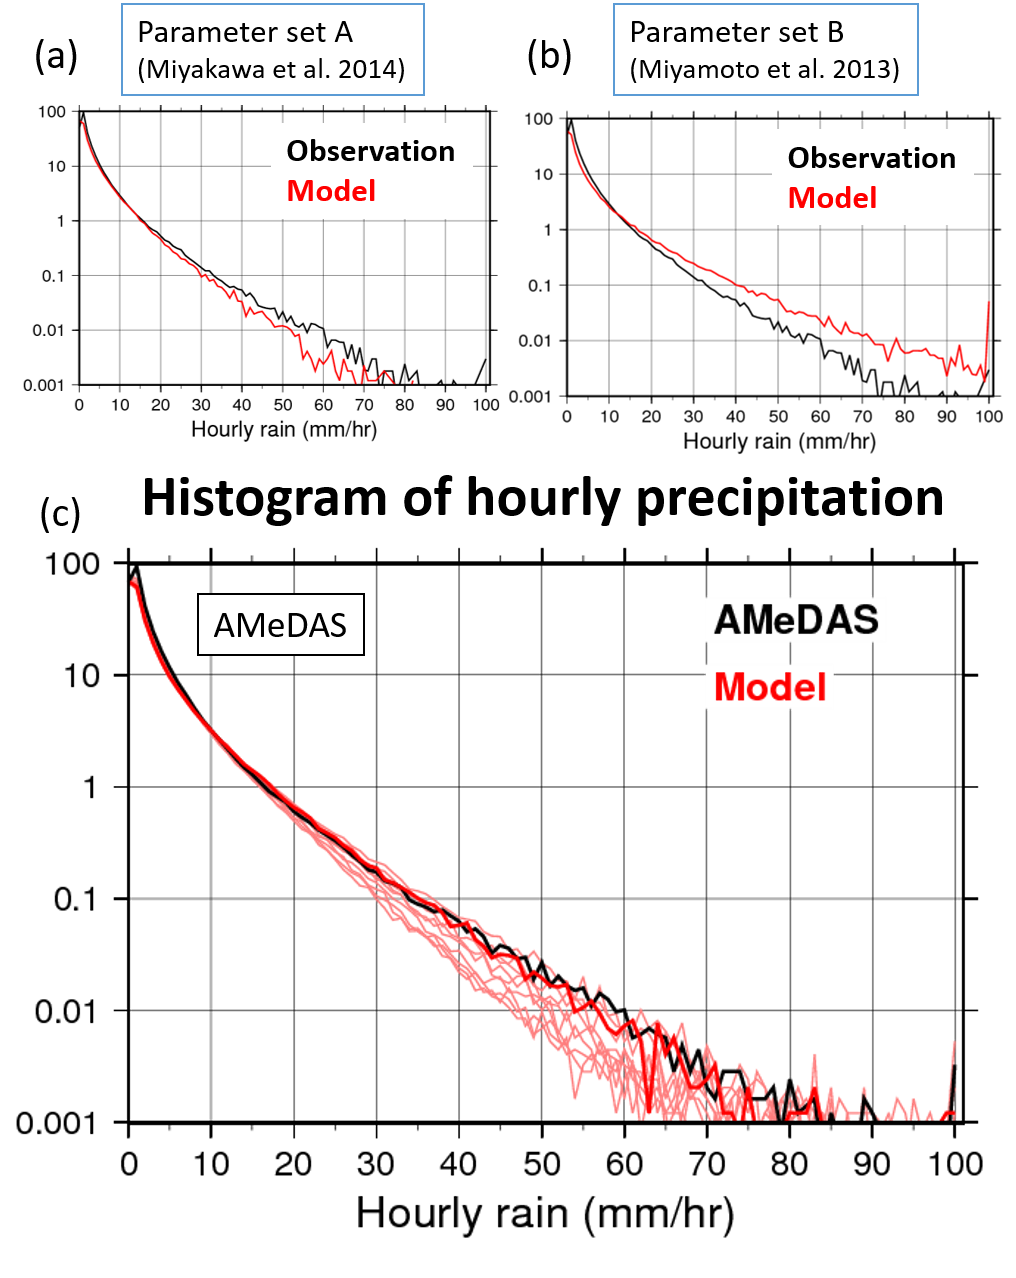
\includegraphics[width=0.5\textwidth,keepaspectratio,natwidth=193,natheight=40]
  {research/tomita/climate-teamFig1.png}
  \caption{Results of microphysics tuning.}
  \locallabel{fig:ctfig1}
\end{figure}


The validation for the physical performance is an important issue as well as code development. In this fiscal year, we tuned the microphysical scheme, focusing on the one-moment bulk method (Tomita et al.2008). Although this scheme was used also in NICAM through the project SPIRE, it depends on the resolution and phenomena we can see. For this purpose, we conducted the series of systematic parameter tuning suitable to Japanese western region using the GSM data as the boundary condition and compared the precipitation with AMeDAS data. Figure \localref{fig:ctfig1} (a) and (b) shows results of hourly precipitation histogram from two typical parameter sets of the microphysics, which has been used in NICAM experiments (Miyakawa et al. 2014, Miyamoto et al.2013). After several key parameters were swept, we successfully tuned the parameters as shown in Fig.\localref{fig:ctfig1} (c).




In this fiscal year, two landmark paper for SCALE was published. The first paper describes the proof-of-concept like study according to SCALE policy (Sato et al. 2015\cite{Sato_et_al_2015}). The three microphysical schemes, the one-moment bulk, two-moment bulk, and spectral bin schemes were compared by sensitivity experiments in which the other components were fixed in SCALE-RM. Since SCALE is targeting to enable self-model inter-comparison easily, this paper is high significant as a SCALE reference paper. The other paper is about the model description of SCALE-RM dynamical core(Nishizawa et al. 2015\cite{Nishizawa_et_al_2015}). In this paper, we reveals that the influence of the grid aspect ratio of horizontal to vertical grid spacing on turbulence in the planetary boundary layer (PBL) in a large-eddy simulation (LES). This paper gives a deep suggestion to meteorological LES. One key point is how the filter length be configured.  It should be based on consideration of the numerical scheme. We also confirmed necessity of a corrective factor for the grid aspect ratio into the mixing length. As shown in Fig.\localref{fig:ctfig2}, these remedy generates the theoretical slope of the energy spectrum; otherwise, spurious energy piling appears at high wave numbers.

\begin{figure}
\centering
  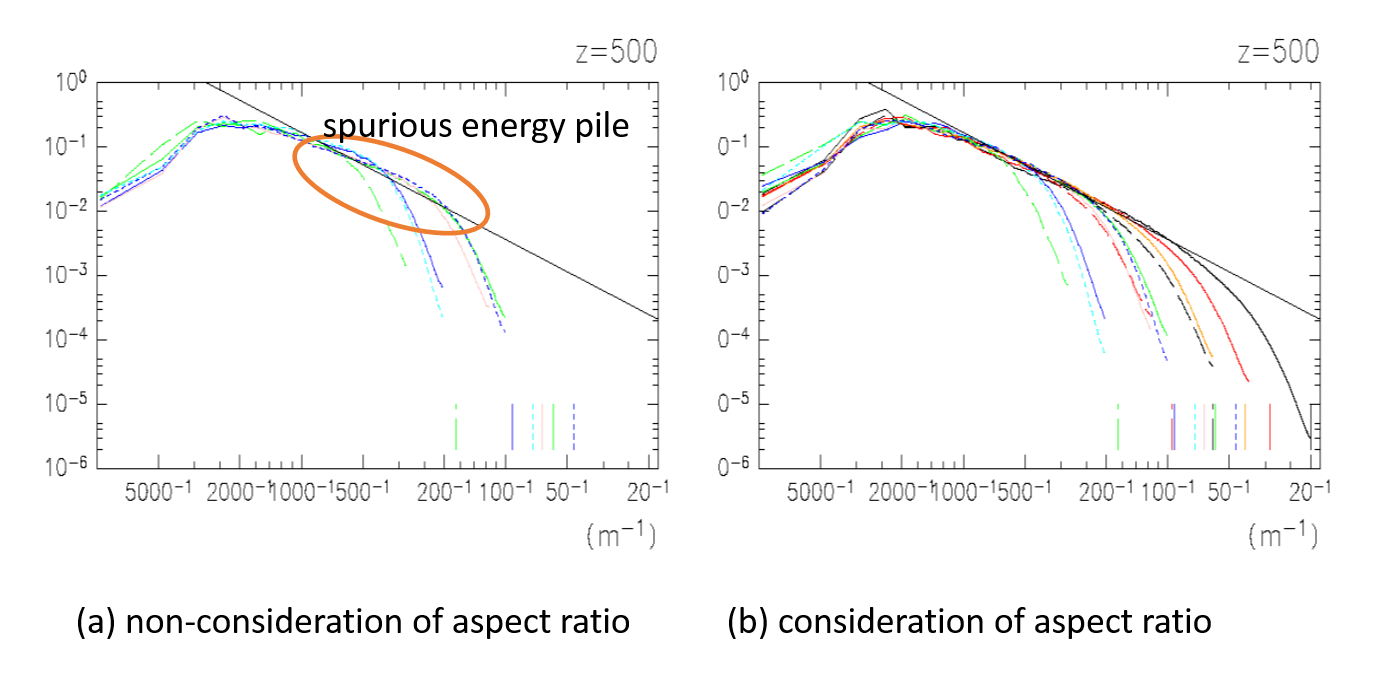
\includegraphics[width=0.8\textwidth,keepaspectratio,natwidth=193,natheight=40]
  {research/tomita/climate-teamFig2.png}
  \caption{The kinetic energy spectrum.}
  \locallabel{fig:ctfig2}
\end{figure}


We investigated also the computational performance of SCALE-RM from the viewpoint of strong scale.  Figure \localref{fig:ctfig4} shows the results of the strong scaling experiments for SCALE-LES. The most time-consuming part is the dynamics, and its scaling factor tends to be saturated by decreasing the problem size. This degradation comes from the increasing ratio of the communication time against the computational time. On the other hand, the scaling of physics gives relatively ideal scaling. In addition, the I/O part is not a bottleneck. To obtain the faster calculation, we implemented several choices both for the temporal and spatial difference schemes. As a result, the longer time step can be obtained in a certain configuration that is 4th order Runge-Kutta scheme in time and 3rd order advection scheme in space.

\begin{figure}
\centering
  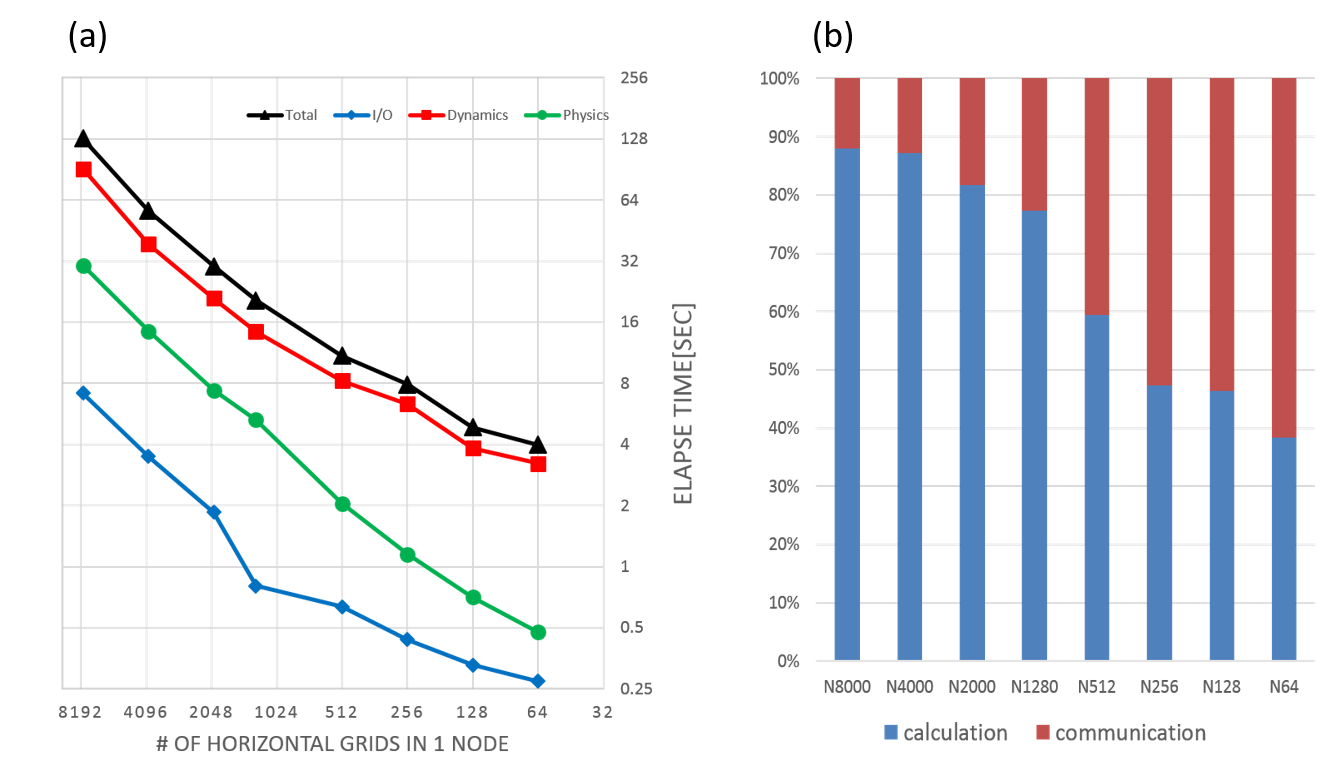
\includegraphics[width=0.8\textwidth,keepaspectratio,natwidth=193,natheight=40]
  {research/tomita/climate-teamFig4.png}
  \caption{(a) Strong scale of SCALE-RM. (b) Ratio of communication to calculation.}
  \locallabel{fig:ctfig4}
\end{figure}


\subsection{Grand challenge run for sub-km horizontal resolution run by global cloud-resolving model}
Using the K computer, we have succeeded in conducting the global simulation with the world’s highest resolution, 870 m, which is published in the 2013 fiscal year (Miyamoto et al. 2013).  In the fiscal year 2015, an additional analyses to reveal the differences in convection properties in various atmospheric disturbances has been done. We focused on the differences in convection under four representative cloudy disturbances: Madden-Julian Oscillation, Tropical Cyclones, Mid-latitudinal Lows, and Fronts (Miyamoto et al. 2015\cite{Miyamoto_et_al_2015x}). In this fiscal year, we summarized the knowledge that we have obtained so far, as a review paper (Kajikawa et al. 2016\cite{Kajikawa_et_al2016}). We conducted further comprehensive analysis of the global-mean state and the characteristics of deep convection, to clarify the difference of the essential change by location and environment. By this paper, this project in our team collaborating with SPIRE was closed once. The subsequent collaboration project leads to the post-K priority project 4.

\subsection{Hyogo-Kobe COE establish project}

In this fiscal year, the boundary conditions inputted to our regional model SCALE-RE was selected. We decided to use the data from the global warming experiments by MRI-AGCM. Figure \localref{fig:ctfig3} (a) shows the target region. Figure \localref{fig:ctfig3} (b) shows the histogram of hourly precipitation of downscaling result, compared with AMeDAS in the present climate. The simulation period is from June to September in 10 years. Owing to the successful model tuning described in the previous section, the observation and model result indicate little difference. Figure \localref{fig:ctfig3} (c) gives comparison between the present and future climates, regarding to the precipitation intensity. The heavy rainfall event increases in the whole Japan area, while the frequency of heavy rainfall is not so changed in the Japanese western area. Figure \localref{fig:ctfig3} (d) shows an expected maximum rainfall intensity that stochastically occurs once twenty years. This result indicates that extreme rainfall occurs in the Kyushu area, but little change occurs in the Kansai area. However, we should note that this result was obtained from just one scenario and one GCM model output; we have to regard this result as one of possible ensembles. For the more reliable result, we should increase the number of scenario and the integration period.

\begin{figure}
\centering
  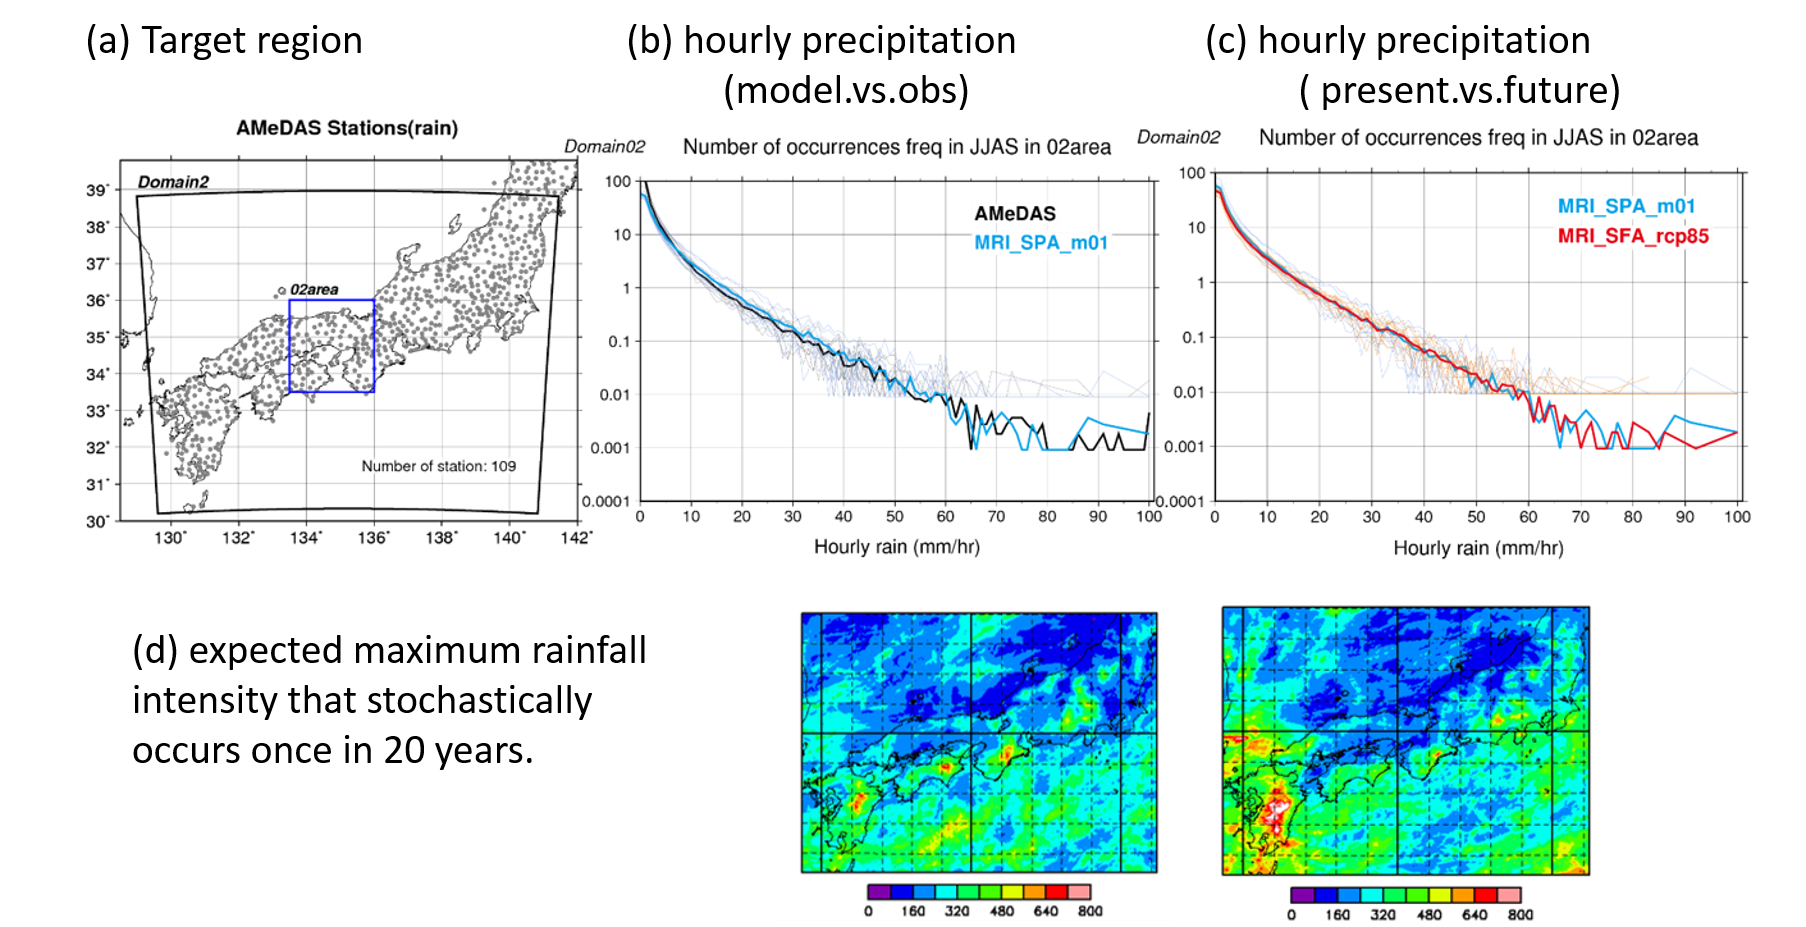
\includegraphics[width=1.0\textwidth,keepaspectratio,natwidth=193,natheight=40]
  {research/tomita/climate-teamFig3.png}
  \caption{The result of the preciptation property in the Japan/Kansai region by the direct downscaling.}
  \locallabel{fig:ctfig3}
\end{figure}


%Text for research Results and achievements. Journal-artcile~\cite{sample-journal}.
%Conference-paper~\cite{sample-conference}.
%Invited-talk~\cite{sample-invited}.
%
%%For cross referencing, use \verb|\locallabel| and \verb|\localref| to avoid conflicting names defined by other groups. For example, a figure can be referenced as Figure~\localref{fig:sample-label1}.

%\begin{figure}
%\centering
%  \includegraphics[width=0.5\textwidth,keepaspectratio,natwidth=193,natheight=40]
%  {sample_division/sample_group/test1.png}
%  \caption{Caption for a sample figure}
%  \locallabel{fig:sample-label1}
%\end{figure}

\section{Schedule and Future Plan}

In the next year, we will continue to further develop, update and maintain the numerical library for the K computer (SCALE library). We also try to enhance the performance of each existing scheme. Especially, validation of cumulus parameterization is necessary. At the same time, we will work on the following three projects in the collaboration with other team in AICS and the scientist in other institute.
\begin{enumerate}
\item On the Hyogo/Kobe COE establish project, we will continue the long-term climate simulation by using SCALE-RM to examine the heavy rainfall over Kobe city area. Several MRI-AGCM results for the future climate is used for increase of scenarios. We will obtain the geographical distribution of the frequency of heavy rainfall and evaluate it more precisely. For this purpose, the pseudo global warming method will be also employed. 
\item We will also contribute to the CREST, Strategic Basic Research Programs “Innovating "Big Data Assimilation" technology for revolutionizing very-short-range severe weather prediction” to develop the main climatological model in SCALE library. In collaboration with the Data Assimilation team in AICS, we developed a prototype of SCALE-LETKF (Local Ensemble Transform Kalman Filter). For this short range forecast, we will pursue both of the computational and physical performance.
\item We join the POST K Science priority project under the collaboration with JAMSTEC. NICAM-LETKF is one of the target applications. Our team will continue to develop and update that application.
\end{enumerate}

%Text for schedule and future plan.
%%
%%


%%% DO NOT EDIT BELOW

\section{Publications}

%\printbibliography[keyword=journal, heading=subbibliography, title={Journal Articles}, prefixnumbers={1-}, resetnumbers=true]
%\printbibliography[keyword=proceedings, heading=subbibliography, title={Conference Papers}, prefixnumbers={2-}, resetnumbers=true]
%\printbibliography[keyword=invited, heading=subbibliography, title={Invited Talks}, prefixnumbers={3-}, resetnumbers=true]
%\printbibliography[keyword=poster, heading=subbibliography, title={Posters and Presentations}, prefixnumbers={4-}, resetnumbers=true]
%\printbibliography[keyword=deliverable, heading=subbibliography, title={Patents and Deliverables}, prefixnumbers={5-}, resetnumbers=true]

\printbibliography[keyword=journal, heading=subbibliography, title={Journal Articles}, resetnumbers=true]
\printbibliography[keyword=proceedings, heading=subbibliography, title={Conference Papers}]
\printbibliography[keyword=invited, heading=subbibliography, title={Invited Talks}]
\printbibliography[keyword=poster, heading=subbibliography, title={Posters and Presentations}]
\printbibliography[keyword=deliverable, heading=subbibliography, title={Patents and Deliverables}]

\end{refsection}

%\begin{refsection}[research/tsubokura/group.bib]
\nocite{*}
\chapter{Complex Phenomena Unified Simulation Research Team}

\section{Members}

\begin{itemize}
  \item[] Makoto Tsubokura (Team Leader)
  \item[] Keiji Onishi (Postdoctoral Researcher)
  \item[] Chung-gang Li (Postdoctoral Researcher) 
  \item[] Leif Niclas Jansson (Postdoctoral Researcher)
  \item[] Rahul Bale (Postdoctoral Researcher)
  \item[] Tetsuro Tamura (Visiting Researcher)
  \item[] Ryoichi Kurose (Visiting Researcher)
  \item[] Gakuji Nagai (Visiting Researcher)
  \item[] Kei Akasaka (Visiting Researcher)
  \end{itemize}

\section{Research Activities}

The objective of our research team is to propose a unified simulation method of solving multiple partial differential equations by developing common fundamental techniques such as the effective algorithms of multi-scale phenomena or the simulation modeling for effective utilization of the massively parallel computer architecture. The target of the unified simulation is supposed to be complex and combined phenomena observed in manufacturing processes in industrial circles and our final goal is to contribute to enhance Japanese technological capabilities and industrial process innovation through the high-performance computing simulation.

Most of the complex flow phenomena observed in manufacturing processes are relating to or coupled with other physical or chemical phenomenon such as turbulence diffusion, structure deformation, heat transfer, electromagnetic field or chemical reaction. While computer simulations are rapidly spreading in industry as useful engineering tools, their limitations to such coupled phenomena have come to realize recently. This is because of the fact that each simulation method has been optimized to a specific phenomenon and once two or more solvers of different phenomena are coupled for such a complicated target, its computational performance is seriously degraded. This is especially true when we utilize a high-performance computer such as K-computer. In such a situation, in addition to the fundamental difficulty of treating different time or spatial scales, interpolation of physical quantities like pressure or velocity at the interface of two different phenomena requires additional computer costs and communications among processor cores. Different mesh topology and hence data structures among each simulation and treatment of different time or spatial scales also deteriorate single processor performance. We understand that one of the keys to solve these problems is to adopt unified structured mesh and data structure among multiple simulations for coupled phenomena. As a candidate of unified data structure for complicated and coupled phenomena, we focused on the building-cube method (BCM) proposed by Nakahashi[1].

\begin{flushleft}
[1]K. Nakahashi, High-Density Mesh Flow Computations with Pre-/Post-Data Compressions, Proc. AIAA 17th CFD Conference (2005) AIAA 2005-4876
\end{flushleft}


\section{Research Results and Achievements}
\subsection{Development of a unified framework for large-scale multiphysics problems}
Based on the Building Cube Method (BCM), we have developed a unified solver framework CUBE (Complex Unified Building cubE) for solving large-scale multphysics problems. The framework has a modular design where CUBE provides a core library containing kernel functionalities e.g. a mesh, flow fields and I/O routines. Solvers are then developed on top of the kernel by connecting necessary kernel modules together, forming a solver pipeline, describing the necessary steps to solve a particular problem.

{\bf Load balancing} is an essential component in today's large scale multiphysics simulations, and with an ever increasing amount of parallelism in modern computer architecture it is essential to reduce even the slightest workload imbalance. An imbalance could severely impact an application's scalability. Traditionally, load balancing is seen as a static problem, closely related to the fundamental problem of parallel computing, namely data decomposition. For a CFD simulation based on BCM, since each cubes contains the same amount of cells the goal is to evenly distribute the cubes among the available cores. However, such a decomposition assumes that the workload for each cube is uniform. For most cubes this is true, but for cubes which contain immersed bodies, combustion, chemical reactions, etc. the workload is slightly higher, which implies a workload imbalance. Therefore, to retain good scalability a load balancing method that balances the workload not only considering the BCM mesh, but also the additional workload from the immersed body, chemical reactions, etc., was developed. 

\begin{figure}[h!]
\centering
  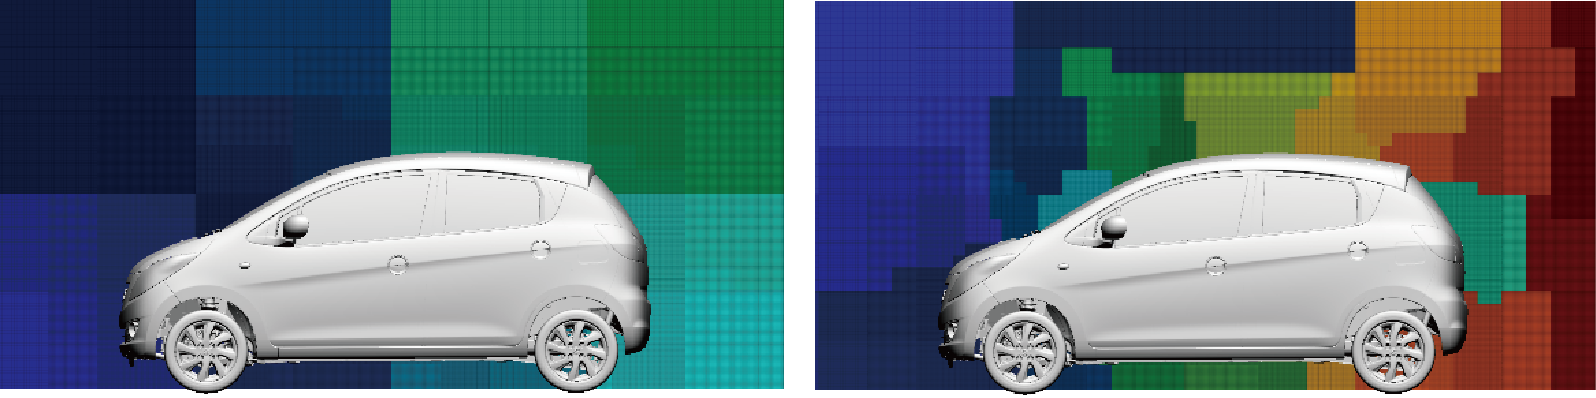
\includegraphics[height=3cm]
  {research/tsubokura/fig1.png}
  \caption{An example of load balancing with respect to the cost of evaluating the immersed geometry and the cost of computing the fluid cells, colored by MPI rank.}
  \locallabel{fig:sample-label1}
\end{figure}


To evaluate the performance of the load balancer, we used CUBE to solve two different incompressible flow problems (full vehicle and a landing gear model) on the K computer. And, the total execution time for performing a fixed number of time steps for both an unbalanced (no load balancing) and a balanced case (using load balancing) on various numbers of cores are compared (Figure~\localref{fig2}).

\begin{figure}[h!]
\centering
  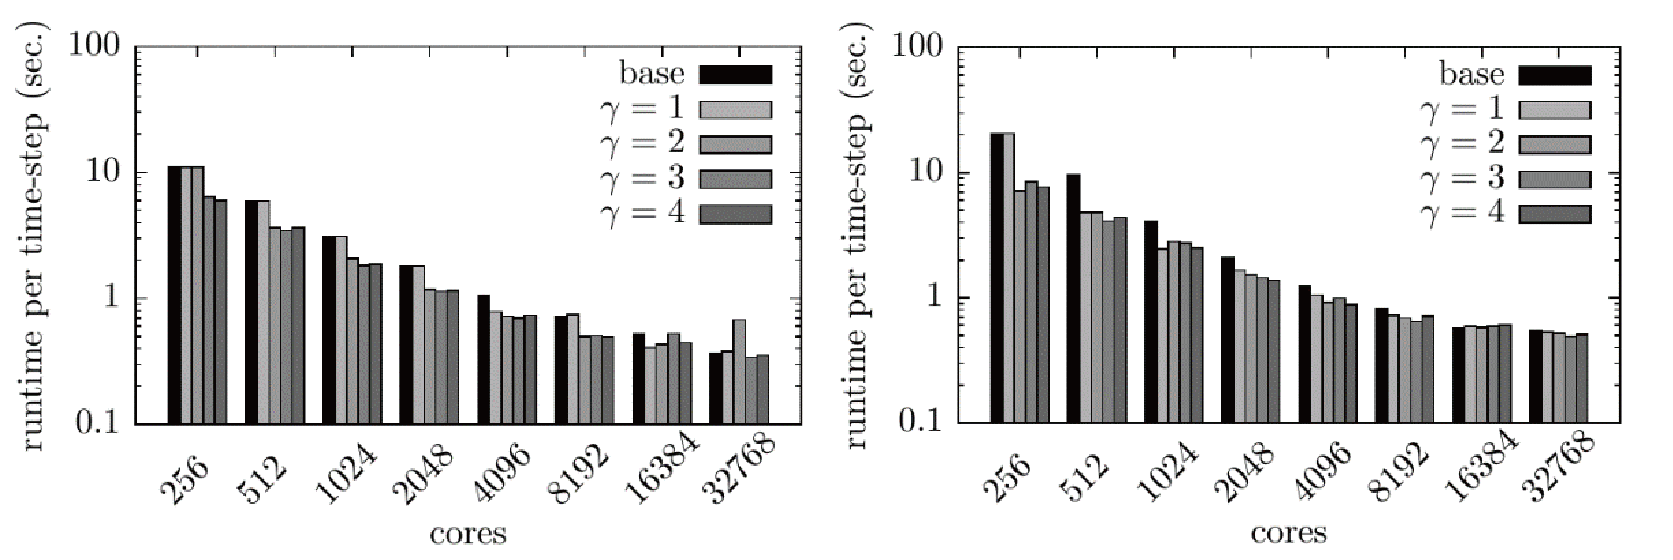
\includegraphics[height=5cm]
  {research/tsubokura/fig2.png}
  \caption{Comparison of  runtime per time-step for balanced and un balanced cases for the landing gear model (left) and the vehicle model (right)}
  \locallabel{fig2}
\end{figure}

\subsection{Development of a very large scale incompressible flow solver with a hierarchical grid system}
The CUBE, name of our software framework, has been developed by conjunction with incompressible flow code which developed to realize the analysis in a real development process of industrial field on the massively parallel environment, including pre- and post-processing. 

{\bf Industrial collaboration, MAZDA}: We have utilized it for the complexed geometrical analysis using dirty CAD data received from automotive company. In last year, we have conducted basic aerodynamics validation using the vehicle geometry of MAZDA Motor Corporation. The conclusion was we need to improve an accuracy of drag force prediction. In this year, we have improved it conducting method survey of interpolation technique onto surface/volume, and the fundamental investigation of approximate domain method on immersed boundary (IB). The difficulty was came from the uncertainty of front/back face of complicated geometry because the interpolation caused huge error if the search of face orientation has been missed. It was highly depends on the complexity of geometry and grid resolution. The method which is drawn by the analogy of Poisson solver providing a front/back face information based on flow solution has been developed. Then we could successfully get a reasonable absolute drag value (about 2\% error), and drag delta between 2 different aerodynamic configurations. At the same time, we could successfully reproduce the characteristic total pressure flow field comparing to wind-tunnel measurement data. 


\begin{figure}[h!]
\centering
  \includegraphics[height=5cm]
  {research/tsubokura/fig3.png}
  \caption{Overview of computational grid and flow field (MAZDA Motor Company).}
  \locallabel{fig3}
\end{figure}

\begin{table}[hbtp]
  \caption{predicted drag on 2 configurations normalized by experimental base case.}
  \label{table1}
  \centering
  \begin{tabular}{lcr}
    \hline
    $C_d$  & Exp.  &  Sim.  \\
    \hline 
    Base  & 1.000  & 1.021 \\
    Aero  & 1.011   & 1.043 \\
    $\Delta C_d$  & 1.15\%  & 1.46\% \\
    \hline
  \end{tabular}
\end{table}

{\bf Industrial collaboration, SUZUKI}: The usability on the practical use of industrial application has been evaluated by discussing with professional engineers of automobile company. we have corroborated with SUZUKI MOTOR CORPORATION to do this work. We have provided CUBE to them with simple documents and training, and they have evaluated by their own way, and gave us their feedback report. The geometry preparation time has been accelerated from 35 hours using commercial software to 2 hours using CUBE framework, based on dirty CAD data. The estimated drag coefficient between 2 configuration had better agreement with measurement than commercial code. It shows CUBE is already ready for usage in the actual design process in term of the usability, human-cost, accuracy, and turn-around time. But, they had a strong request to improve calculation time because their process has a limitation to finish each job within 1 night whereas our method requires 2 or 3 days. To say more, their method is based on Reynold averaged approach based on strong turbulence model which is known to have relatively large error, our method is based on the pure transient approach which generally requires 10 times larger calculation resource comparing to RANS. After the discussion, we have agreed to improve it in near future because it is very important to know the true needs on the field of industrial engineering. As the first step of that, we have developed a new function to enable us to use local refinement grids in the grid generation software. It can reduce the calculation load about from 1/5 to 1/10 for the vehicle case, to accelerate the solution. And the implementation and testing of the local refinement functionality for IB has been started in this year. We thinks it also can lead to the enhancement of effective multi-grid method (MG), or adaptive mesh refinement method (AMR) in the future development scope.

Both of MAZDA and SUZUKI could decide to promote the results inside their organization, and continue the current research activity using our software in FY2016 by submitting the application and accepted the industrial use project on K-computer.

\begin{figure}[h!]
\centering
  \includegraphics[height=5cm]
  {research/tsubokura/fig4.png}
  \caption{Overview of characteristic flow field (SUZUKI MOTOR CORPORATION).}
  \locallabel{fig4}
\end{figure}

\begin{table}[hbtp]
  \caption{predicted drag on 2 configurations normalized by experimental base case.}
  \label{table2}
  \centering
  \begin{tabular}{lcr}
    \hline
    Condition  & CUBE  &  Commercial Code A  \\
    \hline 
Finest grid size	& 2.0 [mm]  &	2.0 [mm] (layer 0.04[mm]) \\
Num. of cells &	400 million & 53 million \\
Fluid Configuration  &	LES (Standard Smagorinsky) & DES (SST k-$\omega$) \\
Num. of timesteps & 145,000 & 4,000 \\
CAD prepare & 8 hours & 8 hours \\
Pre processing time & 2 hours	& 34.5 hours \\
Parallel num. &	4,096 cores (K-computer)  & 512 cores (Intel Xeon) \\
Flow computation time & 258 hours & 8 hours \\
Post processing time & 1.5 hours & 1.2 hours \\
Error of Cd prediction & Applx. 10\% & Applx. 11-16\% \\
Error of $\Delta C_d$  prediction  & 8\%  & 12\% \\
    \hline
  \end{tabular}
\end{table}


{\bf Wind HPC consortium}: At a research activity on Wind-HPC consortium which is organized by Tokyo Institute of Technology and several Japanese major construction companies, the detailed turbulence characteristics on wind canopy of actual urban area geometry that has housings, buildings, vegetation, and street, and so on, has been investigated. And, the academic case validation using square cylinder has been conducted. The results shows reasonable accuracy, so both of results has been published in the paper of architecture design. This research will continue on the FLAGSHIP 2020 project of priority $\sharp$ 4 regarding wind environment evaluation for building construction on severe climate condition through next years.


\begin{figure}[h!]
\centering
  \includegraphics[height=3cm]
  {research/tsubokura/fig5_1.png}
  \caption{Pressure field in Shiodome area(50m Height)}
  \locallabel{fig51}
\end{figure}

\begin{figure}[h!]
\centering
  \includegraphics[height=3cm]
  {research/tsubokura/fig5_3.png}
  \caption{Pressure field in Marunouchi area(50m Height)}
  \locallabel{fig53}
\end{figure}

\begin{figure}[h!]
\centering
  \includegraphics[height=3cm]
  {research/tsubokura/fig5_2.png}
  \caption{Q-criterion (Q=0.0015) in Shiodome area}
  \locallabel{fig52}
\end{figure}

\begin{figure}[h!]
\centering
  \includegraphics[height=3cm]
  {research/tsubokura/fig5_4.png}
  \caption{Q-criterion (Q=0.0015) in Marunouchi }
  \locallabel{fig54}
\end{figure}




\subsection{Development of unified compressible flow solver for unified low to moderate Mach number turbulence with hierarchical grid system}

The Simulation of the low speed compressible turbulence is a key challenge for the industrial applications such as combustion, aeroacoustics and significant heat transfer phenomena. Roe scheme with a low-Mach number fix [1] is adopted to tackle slow flows with variable densities. An immersed boundary method (IBM) for compressible flows with a fast, easy to implement and robust interpolation method is developed to handle the complex geometries.

{\bf Basic Validation with Academic case}: Based on the experiments conducted by Jia and Gogos [2], a steady-state natural convection around a heated sphere under the condition of that, the Grashof number based on the radius of the sphere is 104, is conducted to validate the unified solver. Fig. \localref{fig6a}(a) shows the contour of the velocity magnitude. The entrainment comes from the bottom of the sphere which is consistent with the description by [2]. Fig. \localref{fig6b} shows the temperature contour. Above the top of the sphere, higher temperature region is formed, which cause worse natural convection near the surface so the velocity in this region is quite low. Comparisons of the averaged Nusselt number (Nu), drag coefficients caused by pressure and viscous are tabulated in Table~\localref{tablecdcp}. The results are in good agreement with the experimental data and show the accuracy and availability of our program for dealing with the complex geometry and heat transfer problems. The present results have been published in [3].

\begin{figure}[h!]
\centering
  \includegraphics[height=5cm]
  {research/tsubokura/fig6a.png}
  \caption{A heated sphere: velocity magnitude (m/s) }
  \locallabel{fig6a}
\end{figure}

\begin{figure}[h!]
\centering
  \includegraphics[height=5cm]
  {research/tsubokura/fig6b.png}
  \caption{A heated sphere:  temperature (K)}
  \locallabel{fig6b}
\end{figure}


\begin{table}[hbtp]
  \caption{Comparison with existing experimental data}
  \locallabel{tablecdcp}
  \centering
  \begin{tabular}{cccc}
    \hline
 & $\bar{Nu}$ & $C_{D,p}$ & $C_{D,u}$ \\
    \hline 
Exp. [2] 	& 8.74	& 0.46	& 0.62 \\
Present	& 8.77	& 0.46	& 0.59 \\
    \hline
  \end{tabular}
\end{table}


The simulation of a sphere at Re=104 is performed to investigate the availability of the unified solver for higher Reynolds numbers. Fig. \localref{figmpc} shows the distribution of mean pressure coefficient. The result is well consistent with the [4] and the separation angle can be also accurately captured, which is around 86 degrees.

Fig. \localref{figshcrite} shows the Q criterion contoured by the magnitude of the velocity. The turbulence structures are mainly formed after the separated shear layers generated from the separation point. Besides, the transition from large to small turbulence structures can be also clearly observed in the wake region.

\begin{figure}[h!]
\centering
  \includegraphics[height=5cm]
  {research/tsubokura/fig7a.png}
  \caption{Sphere flow at Re=$10^4$: Distribution of mean pressure coefficient}
  \locallabel{figmpc}
\end{figure}

\begin{figure}[h!]
\centering
  \includegraphics[height=5cm]
  {research/tsubokura/fig7b.png}
  \caption{Sphere flow at Re=$10^4$: Q criterion}
  \locallabel{figshcrite}
\end{figure}


Finally, the simulation of the whole vehicle demonstrates the capability of the unified solver. Fig. \localref{figvelsimvelmag} shows the contour of the velocity magnitude. The development of the boundary layer on the front window and roof can be clearly observed, which shows the capability of unified solver for handling the complex geometry. Besides, the flows penetrate the front of the car to the engine room is also obviously shown, which indicates that our immersed boundary can also treat non-watertight geometry. Fig. \localref{figvstimes} shows the history of the drag and lift coefficients. After reaching the quasi steady state, the average vales of them are good agreement with the experimental data. This is an indication that the unified solver is also able to obtain accurate results for this kind of practical application. In Fig. \localref{figvsflowstr}, the Q-criterion contoured by the magnitude of velocity is shown. The development of turbulent coherent structures near the wheel, mirror and side windows is well captured. In addition, the typical turbulent structures-hair pin can be also obviously observed on the roof. 

\begin{flushleft}
[1] F. Rieper, Journal of Computational Physics, 230 (2011) 5263-5287.

[2] H. Jia, G. Gogos, Int. J. Heat Mass Transfer 19 (1996) 1603-1615.

[3] C. Li, M. Tsubokura, Int. J. Heat Mass Transfer 75 (2016) 52-58.

[4] C. George, S. Kyle, Physics of Fluids, 16 (2004) 1449-1466.
\end{flushleft}

\begin{figure}[h!]
\centering
  \includegraphics[height=3cm]
  {research/tsubokura/fig8a.png}
  \caption{Vehicle Simulation: Snapshot of velocity magnitude}
  \locallabel{figvelsimvelmag}
\end{figure}

\begin{figure}[h!]
\centering
  \includegraphics[height=5cm]
  {research/tsubokura/fig8b.png}
  \caption{Vehicle Simulation: Time series of drag (left) and lift (right) coefficients}
  \locallabel{figvstimes}
\end{figure}

\begin{figure}[h!]
\centering
  \includegraphics[height=6cm]
  {research/tsubokura/fig8c.png}
  \caption{Vehicle Simulation: Snapshot of flow structures extracted by the Q-criterion}
  \locallabel{figvsflowstr}
\end{figure}


\subsection{Development of high performance moving boundary solver for realistic motion}
{\bf Aerodynamics of Vehicle in a turn}: The aerodynamic performance and stability a vehicle is strongly influenced by the crosswinds during cruise and while in turning maneuvers. It is difficult to simulate such real-world flow scenarios in wind tunnel experiments. Furthermore, it is also difficult to measure unsteady aerodynamic forces in wind tunnel experiments. Thus, it is desirable for numerical methods to be able to efficiently and accurately simulate such flow conditions. To this end, here, we present simulation of a vehicle (the complex full vehicle geometry discussed in the previous section) undergoing a turning motion, including wheel rotation and turn, chassis roll and turn, in a uniform flow. This simulation the result of a collaborative work between Mazda Motor Corporation and RIKEN AICS. The detailed vehicle geometry and it motion data were provided by Mazda, and the simulation was carried out at on the K-computer using CUBE. The Lagrangian-Eulerian approach developed during the previous year was used for this simulation. As mentioned above all the vehicle motion, except linear translation, is imposed on the vehicle. If the linear translational motion was imposed on the vehicle, a fine mesh would be needed in the vehicle's path, which makes the mesh size excessively large. An alternate approach, where instead of imposing the linear translation on the vehicle it is imposed on the entire mesh, was used. In this approach the vehicle's center of gravity remains fixed relative to the mesh. So, the fine mesh is needed only in a small region around the vehicle instead of the region of the vehicle's path. This reduced the mesh size by a factor of 3-5.   The results of the simulations are shown in Fig. \localref{figffavitrn}. 

\begin{figure}[h!]
\centering
  \includegraphics[height=4cm]
  {research/tsubokura/fig9.png}
  \caption{Flow field around a vehicle in a turn. (Left) Velocity magnitude on a horizontal plane. (Right) Iso surface of swirl. }
  \locallabel{figffavitrn}
\end{figure}


{\bf Aerodynamic performance of a Ski jumper}: Ski jump is a popular winter sport and is a part of winter Olympics. It is one of the sports in which Japan is competitive and has some of the best ski jumpers in the world. Ski Jump is a sport where aerodynamic interaction of the jumper and air plays a key role in outcome of the sport. Minute changes in an athlete's posture can go a long way, literally.  The distance covered by an athlete is strongly correlated to the drag and lift forces on the athlete while in air. And, these forces are greatly influenced by the athlete's posture. In collaboration with Prof. Keizo Yamamoto of Hokusyo University we investigated the aerodynamic performance of two of Japan's top ski jump athletes, Haruka Iwasa and Sara Takanashi.  Through the unsteady aerodynamic simulation of the two ski jumpers we analyzed the evolution of forces during a short period before and after the jump from the ski ramp. During this period the jumper changes from a sitting posture to a standing posture. Our analysis revealed that the posture and motion of Haruka Iwasa lead to lower drag force and higher lift force compared to the forces on Sara Takanashi. This is consistent with the real-world performance record of the two ski-jumpers.  

\begin{figure}[h!]
\centering
  \includegraphics[height=4.5cm]
  {research/tsubokura/fig10.png}
  \caption{Evolution of flow around Ski jumper Haruka Iwasa during a jump. (Left) Starting posture of the jump. (Right) Final posture of the jump.}
  \locallabel{fig6b}
\end{figure}

\section{Schedule and Future Plan}

\subsection*{(1)Five-year objectives and goals toward 2017}
\begin{itemize}
 \item Construction and development of the simulation technology for bringing out the performance of K-computer
 \item Proposal of the technological trend of HPC simulation toward EXA-scale
\end{itemize}


\subsection*{(2)Long-term objectives}
\begin{itemize}
 \item Establishment of the research and development center for industrial simulation technology
 \item Contribution to computer science by expanding the developed simulation technology to different fields
\end{itemize}


\subsection*{(3)Time schedule}
\begin{figure}[h!]
\centering
  \includegraphics[height=6cm]
  {research/tsubokura/fig11timetable.png}
  \locallabel{fig6b}
\end{figure}

%%% DO NOT EDIT BELOW

\section{Publications}

%\printbibliography[keyword=journal, heading=subbibliography, title={Journal Articles}, prefixnumbers={1-}, resetnumbers=true]
%\printbibliography[keyword=proceedings, heading=subbibliography, title={Conference Papers}, prefixnumbers={2-}, resetnumbers=true]
%\printbibliography[keyword=invited, heading=subbibliography, title={Invited Talks}, prefixnumbers={3-}, resetnumbers=true]
%\printbibliography[keyword=poster, heading=subbibliography, title={Posters and Presentations}, prefixnumbers={4-}, resetnumbers=true]
%\printbibliography[keyword=deliverable, heading=subbibliography, title={Patents and Deliverables}, prefixnumbers={5-}, resetnumbers=true]

\printbibliography[keyword=journal, heading=subbibliography, title={Journal Articles}, resetnumbers=true]
\printbibliography[keyword=proceedings, heading=subbibliography, title={Conference Papers}]
\printbibliography[keyword=invited, heading=subbibliography, title={Invited Talks}]
\printbibliography[keyword=poster, heading=subbibliography, title={Posters and Presentations}]
\printbibliography[keyword=deliverable, heading=subbibliography, title={Patents and Deliverables}]

\end{refsection}

\begin{refsection}[research/maruyama/group.bib]
\nocite{*}
\chapter{HPC Programming Framework Research Team}

\section{Members}

\begin{itemize}
  \item[] Naoya Maruyama (Team Leader)
  \item[] Motohiko Matsuda (Research Scientist)
  \item[] Shinichiro Takizawa (Research Scientist)
  \item[] Mohamed Wahib (Postdoctoral Researcher)
  \item[] Keisuke Fukuda (Research Associate)
  \item[] Koji Ueno (Student Trainee)
  \item[] An Huynh (Student Trainee)
  \item[] Satoshi Matsuoka (Senior Visiting Scientist)
  \item[] Tomoko Nakashima (Assistant)
  \item[] Aya Motohashi (Assistant)
\end{itemize}

Text for research Results and achievements. Journal-artcile~\cite{sample-journal}.
Conference-paper~\cite{sample-conference}.
Invited-talk~\cite{sample-invited}.

For cross referencing, use \verb|\locallabel| and \verb|\localref| to avoid conflicting names defined by other groups. For example, a figure can be referenced as Figure~\localref{fig:sample-label1}.

\begin{figure}
\centering
  \includegraphics[width=0.5\textwidth,keepaspectratio,natwidth=193,natheight=40]
  {sample_division/sample_group/test1.png}
  \caption{Caption for a sample figure}
  \locallabel{fig:sample-label1}
\end{figure}

\section{Research Activities}

We develop high performance, highly productive software stacks that aim to simplify development of highly optimized, fault-tolerant computational science applications on current and future supercomputers, notably the K computer. Our current focus of work includes large-scale data processing, heterogeneous computing, and fault tolerance. A major ongoing project in our group will deliver a MapReduce runtime that is highly optimized for the intra- and inter-node architectures of the K computer as well as its peta-scale hierarchical storage systems. Another major project focuses on performance and productivity in large-scale heterogeneous systems. We also study high performance graph analytics on the K computer. Below is a brief summary of each project.

\section{Research Results and Achievements}

\subsection{KMR}
% Takizawa & Matsuda
\subsubsection{Improve locality when running MPI programs as MapReduce tasks}

Although MapReduce systems can allocate tasks to nodes where their inputs reside to increase data locality for improving performance, these systems only target on tasks implemented as serial programs and do not consider running tasks implemented as parallel programs using MPI as Map or Reduce task.
As many scientific applications are implemented using MPI and some application workflows form ensemble execution patterns of such MPI programs, the workflows can be implemented easily and efficient data access can be achieved if a MapReduce system can allocate tasks implemented using MPI so that it can exploit data locality in them.

We proposed an extension of the execution model of MapReduce to achieve high performance when running MPI programs as Map/Reduce tasks.
We model data to be processed as Key-Value as the traditional MapReduce model.
However, to processing the data, we propose a new \verb|map| function which makes process groups where each process in a group has a key-value whose key is same as those of other processes in the group and applies a user-defined mapper, which is implemented using MPI, to the key-values using processes in each group.

\begin{figure}
\centering
  \includegraphics[width=0.5\textwidth,keepaspectratio,natwidth=193,natheight=40]
  {research/maruyama/lo01.png}
%  \caption{Caption for a sample figure}
  \locallabel{fig:kmr-01}
\end{figure}

To evaluate our proposal, we used $N \times N$ nodes of the K computer and compared performance of our method in which data access was performed locally and that of random data access.
We used a synthetic benchmark program where each node has an individual data and which iterates the following two computation; the first computation groups $N$ nodes in low direction and processes data on them, and the second groups $N$ nodes in column direction and processes data on them.
The result is shown in the figure.
The horizontal axis is the amount of data on each node and the virtical axis is the relative performance of an iteration against random data access.
As can be seen from the figure, the performance of our proposal improve as the number of nodes and the amount of data increase.

\begin{figure}
\centering
  \includegraphics[width=0.5\textwidth,keepaspectratio,natwidth=193,natheight=40]
  {research/maruyama/lo02.png}
%  \caption{Calculation pattern of the benchmark program}
  \locallabel{fig:kmr-02}
\end{figure}

\begin{figure}
\centering
  \includegraphics[width=0.5\textwidth,keepaspectratio,natwidth=193,natheight=40]
  {research/maruyama/lo03.png}
%  \caption{Experimental results}
  \locallabel{fig:kmr-03}
\end{figure}


\subsubsection{Skew-tuned shuffling for load balancing for Reduce operation}

In a MapReduce program, the number of tasks 


\subsubsection{Visualize MapReduce task execution}

\begin{figure}
\centering
  \includegraphics[width=0.5\textwidth,keepaspectratio,natwidth=193,natheight=40]
  {research/maruyama/kmrviz.png}
  \caption{Caption for a sample figure}
  \locallabel{fig:kmrviz}
\end{figure}


\subsubsection{Apache Spark on K computer}


\subsection{High Level Framework for High Performance AMR}
% Wahib

\subsection{High Performance Graph Analytics Study with Graph500}
% Maruyama

\section{Schedule and Future Plan}

\subsection{KMR}
% Takizawa & Matsuda

\subsection{High Level Framework for High Performance AMR}
% Wahib

\subsection{High Performance Graph Analytics Study with Graph500}
% Maruyama

%%% DO NOT EDIT BELOW

\section{Publications}

%\printbibliography[keyword=journal, heading=subbibliography, title={Journal Articles}, prefixnumbers={1-}, resetnumbers=true]
%\printbibliography[keyword=proceedings, heading=subbibliography, title={Conference Papers}, prefixnumbers={2-}, resetnumbers=true]
%\printbibliography[keyword=invited, heading=subbibliography, title={Invited Talks}, prefixnumbers={3-}, resetnumbers=true]
%\printbibliography[keyword=poster, heading=subbibliography, title={Posters and Presentations}, prefixnumbers={4-}, resetnumbers=true]
%\printbibliography[keyword=deliverable, heading=subbibliography, title={Patents and Deliverables}, prefixnumbers={5-}, resetnumbers=true]

\printbibliography[keyword=journal, heading=subbibliography, title={Journal Articles}, resetnumbers=true]
\printbibliography[keyword=proceedings, heading=subbibliography, title={Conference Papers}]
\printbibliography[keyword=invited, heading=subbibliography, title={Invited Talks}]
\printbibliography[keyword=poster, heading=subbibliography, title={Posters and Presentations}]
\printbibliography[keyword=deliverable, heading=subbibliography, title={Patents and Deliverables}]

\end{refsection}

\begin{refsection}[research/ono/group.bib]
\nocite{*}
\chapter{Advanced Visualization Research Team}

\section{Members}

\begin{itemize}
  \item[] Ichiro Kobe (Team Leader)
  \item[] Jiro Kobe (Senior Scientist)
  \item[] Saburo Kobe (Research Scientist)
\end{itemize}

\section{Research Activities}

Text for research activities.

\section{Research Results and Achievements}

Text for research Results and achievements. Journal-artcile~\cite{sample-journal}.
Conference-paper~\cite{sample-conference}.
Invited-talk~\cite{sample-invited}.

For cross referencing, use \verb|\locallabel| and \verb|\localref| to avoid conflicting names defined by other groups. For example, a figure can be referenced as Figure~\localref{fig:sample-label1}.

\begin{figure}
\centering
  \includegraphics[width=0.5\textwidth,keepaspectratio,natwidth=193,natheight=40]
  {sample_division/sample_group/test1.png}
  \caption{Caption for a sample figure}
  \locallabel{fig:sample-label1}
\end{figure}

\section{Schedule and Future Plan}

Text for schedule and future plan.

%%% DO NOT EDIT BELOW

\section{Publications}

%\printbibliography[keyword=journal, heading=subbibliography, title={Journal Articles}, prefixnumbers={1-}, resetnumbers=true]
%\printbibliography[keyword=proceedings, heading=subbibliography, title={Conference Papers}, prefixnumbers={2-}, resetnumbers=true]
%\printbibliography[keyword=invited, heading=subbibliography, title={Invited Talks}, prefixnumbers={3-}, resetnumbers=true]
%\printbibliography[keyword=poster, heading=subbibliography, title={Posters and Presentations}, prefixnumbers={4-}, resetnumbers=true]
%\printbibliography[keyword=deliverable, heading=subbibliography, title={Patents and Deliverables}, prefixnumbers={5-}, resetnumbers=true]

\printbibliography[keyword=journal, heading=subbibliography, title={Journal Articles}, resetnumbers=true]
\printbibliography[keyword=proceedings, heading=subbibliography, title={Conference Papers}]
\printbibliography[keyword=invited, heading=subbibliography, title={Invited Talks}]
\printbibliography[keyword=poster, heading=subbibliography, title={Posters and Presentations}]
\printbibliography[keyword=deliverable, heading=subbibliography, title={Patents and Deliverables}]

\end{refsection}

\begin{refsection}[research/miyoshi/group.bib]
\nocite{*}
\chapter{Data Assimilation Research Team}

\section{Members}

\begin{itemize}
\item[] Takemasa Miyoshi (Team Leader)
\item[] Koji Terasaki (Research Scientist)
\item[] Shigenori Otsuka (Postdoctoral Researcher)
\item[] Keiichi Kondo (Postdoctoral Researcher)
\item[] Shunji Kotsuki (Postdoctoral Researcher)
\item[] Guo-Yuan Lien (Postdoctoral Researcher)
\item[] Takumi Honda (Postdoctoral Researcher)
\item[] Yasumitsu Maejima (Research Associate)
\item[] Africa Perianez Santiago (Research Associate)
\item[] Hazuki Arakida (Technical Staff)
\item[] Gulanbaier Tuerhong (Technical Staff)
\item[] Juan J. Ruiz (Visiting Scientist)
\item[] Shinichiro Shima (Visiting Scientist)
\item[] Shu-Chih Yang (Visiting Scientist)
\item[] Stephen G. Penny (Visiting Scientist)
\item[] Masaru Kunii (Visiting Scientist)
\item[] Kozo Okamoto (Visiting Scientist)
\item[] Michiko Otsuka (Visiting Scientist)
\item[] Marimo Ohhigashi (Research Assistant)
\item[] Yaping Chang (International Program Associate)
\item[] Yukie Komori (Assistant)
\item[] Rie Deguchi (Assistant)
\end{itemize}

\section{Research Activities}

The Data Assimilation Research Team (DA Team) was launched in October 2012 and is composed of 18 research and technical staff including 7 visiting members as of March 2016. Data assimilation (DA) is a cross-disciplinary science to synergize computer simulations and real-world data, based on statistical mathematics and dynamical systems theory. As computers advance and enable precise simulations, it will become more important to compare the simulations with real-world data. DA Team performs cutting-edge research and development on advanced DA methods and their wide applications, aiming to integrate computer simulations and real-world data in the wisest way. Particularly, DA Team tackles challenging problems of developing efficient and accurate DA systems for ``big simulations'' with real-world ``big data'' from various sources including advanced sensors. The specific foci include 1) theoretical and algorithmic developments for efficient and accurate DA, 2) DA methods and applications by taking advantage of the world-leading K computer and ``big data'' from new advanced sensors, and 3) exploratory new applications of DA in wider simulation fields. These advanced DA studies will enhance simulation capabilities and lead to a better use of high-performance computers including the leading-edge K computer.

In FY2015, we continued on the ongoing data assimilation research in the following aspects: 1) theoretical research on challenging problems, 2) leading research on meteorological applications, 3) optimization of computational algorithms, and 4) exploratory research on wider applications. We also continued close collaborations with several research teams within the AICS Research Division. We have made substantial progress on the following research items:


\paragraph{Theoretical research}
\begin{itemize}
  \setlength{\parskip}{0cm}
  \setlength{\itemsep}{0cm}

\item A paper on the discrete Bayesian optimization approach to find optimal ensemble sizes in a multi-model ensemble Kalman filter (EnKF) was published (1 paper published).

\item A new local particle filter method to treat non-Gaussian PDF was explored (1 paper submitted).
\end{itemize}

\paragraph{Leading research on meteorological applications}
\begin{itemize}
  \setlength{\parskip}{0cm}
  \setlength{\itemsep}{0cm}

\item We have successfully run the largest-ever ensemble DA experiments with 10,240 samples for the global atmosphere using real observations with the real-case Nonhydrostatic ICosahedral Atmospheric Model (NICAM) (1 paper published, press release on November 11, 2015).

\item Impact of localization in ensemble Kalman filter was investigated with 10,240 samples using an intermediate AGCM (1 paper submitted).

\item Non-Gaussian statistics in the global atmospheric dynamics were investigated with the 10,240-sample ensemble Kalman filter using an intermediate AGCM.

\item Multi-scale data assimilation was investigated based on 10,240-member ensemble Kalman filter using an intermediate AGCM and NICAM.

\item A DA system for Advanced Microwave Sounding Unit (AMSU)-A radiance data was developed with NICAM-LETKF.

\item A DA system for JAXA's Global Satellite Mapping of Precipitation (GSMaP) data was developed with NICAM-LETKF.

\item A high resolution experiment using NICAM-LETKF system assimilating the conventional, AMSU-A, and GSMaP observations has been performed on the K computer.

\item The spatial and inter-channel observation error correlations of AMSU-A were investigated with the NICAM-LETKF system.

\item An earlier study on the assimilation of global precipitation data with the low-resolution NCEP GFS model were summarized and published (2 papers published).

\item A paper on the new quality control algorithm for the Osaka Phased Array Weather Radar (PAWR) was published (1 paper published).

\item The LETKF system with the SCALE model (SCALE-LETKF) was developed and improved in collaboration with Computational Climate Science Research Team. Several new functions,
  including PAWR assimilation, Himawari-8 satellite data assimilation,
  relaxation-to-prior-spread (RTPS) method, offline-nested domains, were implemented with the SCALE-LETKF system.

\item A near-real-time regional weather analysis and forecast system based on the SCALE-LETKF has been set up and run on the K computer.
  It has produced weather analyses and 5-day forecasts every 6 hours for more than 9 months.

\item The ``Big Data Assimilation'' experiments for a local severe rainstorm case were performed with the SCALE-LETKF system, assimilating the PAWR data.
  The results were compared with the previous NHM-LETKF experiments and the nowcasting experiments (1 paper submitted).

\item A project-wide paper for ``Big Data Assimilation'' with the first results of NHM-LETKF experiments was accepted for publication (1 paper accepted).

\item Model output statistics have been investigated using machine learning algorithms and deep learning algorithms.

\item Convective predictability was investigated by performing breeding experiments. Dependency on the model resolution was investigated.

\item A precipitation nowcasting system was developed to take advantage of the dense and frequent PAWR data (1 paper published).

\item A space-time extrapolation system for GSMaP with DA was developed using LETKF.
  The system has been running in real time since January 2016 (1 paper accepted in June 2016).

\item A new Himawari-8 observation operator for SCALE-LETKF was developed and tested with a tropical cyclone case.

\item Himawari-8 may capture clouds at an earlier stage of convective development before a radar captures large raindrops. This potential advantage was explored.

\item The potential usage of Himawari-8 observation for estimating microphysics parameters through DA was explored.

\item A 4-dimensional NHM-LETKF system was developed to investigate a fail-safe workflow and the relationship between the DA window length and forecast accuracy.

\item A series of DA experiments for a sudden local severe rainstorm case in Kobe on September 11, 2014 was performed to investigate the predictability.
\end{itemize}

\paragraph{Computational optimization}

\begin{itemize}
  \setlength{\parskip}{0cm}
  \setlength{\itemsep}{0cm}

\item Huge-jobs, computing the ``Big Data Assimilation'' problem with the SCALE-LETKF, as big as near full nodes of the K computer were performed to measure the computational time and scalability of the code.

%\item Large ensemble

%\item The computational performance of NICAM-LETKF was improved in collaboration with the Computational Climate Science Research Team (1 paper published).
\end{itemize}

\paragraph{Wider applications}

\begin{itemize}
  \setlength{\parskip}{0cm}
  \setlength{\itemsep}{0cm}

\item A particle filter was applied to a dynamical vegetation model known as the SEIB-DGVM (Spatially-Explicit, Individual-Based Dynamic Global Vegetation Model).
  Uncertainties in the state variables and the parameters were greatly reduced by assimilating satellite based Leaf Area Index.

\item Land surface DA system was developed with SiBUC (Simple Biosphere including Urban Canopy) model and LETKF.

\item A global crop calendar was estimated with the satellite-sensed vegetation index (1 paper published).

\item Impacts of satellite-based solar radiation data on land surface simulations were estimated (1 paper published).
\end{itemize}

Several achievements are selected and highlighted in the next section.

\section{Research Results and Achievements}


\subsection{Big Ensemble Data Assimilation in Numerical Weather Prediction}
\locallabel{sec:big_ensemble_da}
Taking advantage of the K computer,
we have successfully run the largest-ever ensemble DA experiments with 10,240 samples for the global atmosphere
with the real-case Nonhydrostatic ICosahedral Atmospheric Model (NICAM) (Miyoshi et al. 2015)
using the NICAM-LETKF (Local Ensemble Transform Kalman Filter) system developed in FY2014 (Terasaki et al. 2015).
This research result was highlighted by RIKEN Press Release on November 11, 2015.
The samples size of 10,240 is two orders of magnitude larger than the typical choice of about 100. The computational cost for the ensemble DA is proportional to the cubic power of the sample size, and active collaborations with AICS Large-scale Parallel Numerical Computing Technology Research Team (PI: Dr. T. Imamura) played an essential role in accelerating the computation by a factor of 8 using an eigenvalue solver “EigenExa” optimized for the K computer. The large sample size reduces the sampling error (Fig. \localref{fig:1}), and we discovered potential long-range correlations up to about 7,000 km (Fig. \localref{fig:1} b). This suggests potential use of faraway observations to improve numerical weather prediction (NWP), although we usually assume that the impact of observations is limited within a range up to 4,000 km or so. The large ensemble DA experiments would provide fundamental datasets to improve our knowledge on the flow-dependent error statistics including non-Gaussian and multi-scale structures, and would help develop advanced approaches for non-Gaussian and multi-scale DA, the topics at the center of theoretical DA research.

\begin{figure}
\centering
  \includegraphics[width=0.99\textwidth,keepaspectratio,natwidth=193,natheight=40,clip,trim=0 240 0 0]
  {research/miyoshi/miyoshi-team-fig1.png}
  \caption{Horizontal maps of real atmosphere autocorrelations with (a) 80 samples and (b) 10240 samples. Adopted from Fig. 5 of Miyoshi et al. (2015), \copyright IEEE 2015.}
  \locallabel{fig:1}
\end{figure}

\subsection{Near-real-time Implementation of Regional Numerical Weather Prediction (NWP)}
The LETKF-based DA system has been newly developed with the regional NWP model ``SCALE'' in collaboration with Computational Climate Science Research Team (PI: Dr. H. Tomita). Real-world observation data are available from the US National Centers for Environmental Prediction (NCEP) in near real time, by about 3-hour delay from the real time. We have implemented the near-real-time 5-day NWP using the SCALE-LETKF system, and have been running continuously from May 7, 2015. Figure \localref{fig:3} indicates an example of a forecast in a case of the worst disaster in 2015 by flooding of River Kinugawa, Tochigi, Japan. The line-type system is well simulated. By continuously running SCALE-LETKF analysis and forecasts, we accumulate experiences and verification samples, which will be very useful for further improvements of DA and NWP system developments.

\begin{figure}
\centering
  \includegraphics[width=0.99\textwidth,keepaspectratio,natwidth=193,natheight=40]
  {research/miyoshi/miyoshi-team-fig3.png}
  \caption{1-hour accumulated rainfall amount at 0000 JST, September 10, 2015, when River Kinugawa had flooded and caused severe disasters, from a model simulation initiated at 1200 JST, September 8 (left) and surface rain-gauge observation (right) from NTT Docomo environmental sensor network.}
  \locallabel{fig:3}
\end{figure}

\subsection{Effective Use of Satellite Big Data}
Developing DA methods for effective use of various observation data is important. Satellite remote sensing provides a relatively uniform coverage of a broad area of the globe, and plays an essential role in NWP. However, the observed quantities are not direct to the prognostic variables of NWP models, and the data volume and variety keep increasing rapidly as sensor technology advances. Therefore, satellite DA requires algorithmic and methodological developments, and has become a major field in meteorology. We have been actively working on the research on effective assimilation of satellite-based precipitation data including the GPM (global precipitation measuring mission) core satellite data in collaboration with JAXA (Japan Aerospace Exploration Agency), microwave radiances from low-earth orbit satellites, and big data from the new-generation geostationary satellite Himawari-8 in collaboration with JMA (Japan Meteorological Agency) Meteorological Satellite Center and Meteorological Research Institute. Figure \localref{fig:4} shows an example of the impact of assimilating Himawari-8 infrared radiances in the case of Typhoon Soudelor 2015. The outer rainbands north of the vortex are greatly enhanced by assimilating Himawari-8 and becomes much closer to the observation.


\begin{figure}
\centering
  \includegraphics[width=0.99\textwidth,keepaspectratio,natwidth=193,natheight=40,clip,trim=0 230 0 0]
  {research/miyoshi/miyoshi-team-fig4.png}
  \caption{Geostationary satellite Himawari-8 band-14 brightness temperature (K) at 1510 UTC, August 2, 2015 (right) and simulated images with/without assimilating Himawari-8 data (center/left).}
  \locallabel{fig:4}
\end{figure}

\subsection{New Application with Individual-based Dynamical Vegetation Model}
As a new explorative application of DA, we have been working on land-surface and vegetation applications. We have successfully applied DA to the Spatially-Explicit Individual-Based Dynamic Global Vegetation Model (SEIB-DGVM) for the first time. The individual-based model simulates individual plants explicitly; some trees may die, while new trees may emerge. Therefore, the model prognostic variables such as tree height and root depth may change time to time and place to place. Typical DA methods assume the phase space to be predefined and never change. Alternatively, we applied a SIR (Sequential Importance Resampling) particle filter. The results were encouraging. Figure \localref{fig:5} shows the results with the real satellite-based MODIS (Moderate Resolution Imaging Spectroradiometer) LAI (Leaf Area Index) observations at a single location. It is not surprising that the uncertainties of the simulated LAI are reduced significantly (Fig. \localref{fig:5} a), but we also find that the uncertainties of unobserved model parameters and variables are reduced significantly (Fig. \localref{fig:5} b, c).

\begin{figure}
\centering
  \includegraphics[width=0.99\textwidth,keepaspectratio,natwidth=193,natheight=40]
  {research/miyoshi/miyoshi-team-fig5.png}
  \caption{4-year time series of (a) LAI, (b) a model parameter (maximum photosynthesis rate), and (c) a model variable (net ecosystem exchange) for the cases without DA (left) and with DA (right). Adopted from Arakida et al. (2016, \textit{Nonlin.\ Processes Geophys.\ Discuss.}).}
  \locallabel{fig:5}
\end{figure}

\subsection{Theoretical and algorithmic developments}
\locallabel{sec:theoretical}
Theoretical DA research is an important part of DA Team’s scope. Here, we highlight some of the major theoretical developments in FY2015.
A paper on the discrete Bayesian optimization approach to find optimal ensemble sizes in a multi-model ensemble Kalman filter (EnKF) was published (Otsuka and Miyoshi 2015).
Potential impact of assimilation order of observations in serial EnKF was investigated (Kotsuki et al., manuscript in preparation).
A new local particle filter method to treat non-Gaussian PDF was explored (Penny and Miyoshi 2016, \textit{Nonlin.\ Processes Geophys.\ Discuss.}).


%Text for research Results and achievements. Journal-artcile~\cite{sample-journal}.
%Conference-paper~\cite{sample-conference}.
%Invited-talk~\cite{sample-invited}.
%For cross referencing, use \verb|\locallabel| and \verb|\localref| to avoid conflicting names defined by other groups. For example, a figure can be referenced as Figure~\localref{fig:sample-label1}.

%\begin{figure}
%\centering
%  \includegraphics[width=0.5\textwidth,keepaspectratio,natwidth=193,natheight=40]
%  {sample_division/sample_group/test1.png}
%  \caption{Caption for a sample figure}
%  \locallabel{fig:sample-label1}
%\end{figure}

\section{Schedule and Future Plan}

In FY2015, DA team had one additional full-time research staff, and the team will grow further in FY2016.
DA team has been exploring various aspects of DA including theoretical problems, meteorological applications, and wider applications,
with large-scale computing to fully utilize ``Big Data.''
We have very strong projects in weather forecast applications supported by the JST CREST program, JAXA, and MEXT FLAGSHIP 2020 project.
We will continue our efforts in each topic in FY2016.

``Big Data Assimilation'' (BDA) is one of the major activities that we have developed in FY2015.
The prototype system showed promising results, but the computing speed with the K computer did not meet the requirement for real-time implementation.
Also, the physical performance for the 30-minute forecast of precipitation patterns needs to be improved.
In FY2016, we will continue to work on the development of the BDA system to further improve the computational and physical performances.

In FY2016, we also plan to enhance close collaborations with experts in mathematics, sensor technology, and various application fields.
Enhancing collaborations with other AICS Research Teams will also be beneficial.


\section{Publications}
\section*{Journal Articles}
\begin{enumerate}
  \renewcommand*\labelenumi{[\theenumi]}
\item
  Lien, G.-Y., T. Miyoshi, and E. Kalnay: ``Assimilation of TRMM Multisatellite Precipitation Analysis with a low-resolution NCEP Global Forecast System'', Mon. Wea. Rev., Vol.144, p.643--661, 2016.
\item
  Lien, G.-Y., E. Kalnay, T. Miyoshi, and G. J. Huffman: ``Statistical properties of global precipitation in the NCEP GFS model and TMPA observations for data assimilation'', Mon. Wea. Rev., Vol.144, p.663--379, 2016.
\item
  Otsuka, S., G. Tuerhong, R. Kikuchi, Y. Kitano, Y. Taniguchi, J. J. Ruiz, S. Satoh, T. Ushio, and T. Miyoshi: ``Precipitation nowcasting with three-dimensional space-time extrapolation of dense and frequent phased-array weather radar observations'', Weather and Forecasting, Vol.31, p.329--340, 2016.
\item
  Dillon, M. E., Y. G. Skabar, J. Ruiz, E. Kalnay, E. A. Collini, P. Echevarr\'{i}a, M. Saucedo, T. Miyoshi, and M. Kunii: ``Application of the WRF-LETKF Data Assimilation System over Southern South America: Sensitivity to model physics'', Weather and Forecasting, Vol.31, p.217--236, 2016.
\item
  Hattori, M., J. Matsumoto, S. Ogino, T. Enomoto, and T. Miyoshi: ``The Impact of Additional Radiosonde Observations on the Analysis of Disturbances in the South China Sea during VPREX2010'', SOLA, Vol.12, p.75--79, 2016.
\item
  Sluka, T. C., S. G. Penny, E. Kalnay, and T. Miyoshi: ``Assimilating atmospheric observations into the ocean using strongly coupled ensemble data assimilation'', Geophys. Res. Lett., Vol.43, p.752--759, 2016.
\item
  Sueyoshi T., K. Saito, S. Miyazaki, J. Mori, T. Ise, H. Arakida, R. Suzuki, A. Sato, Y. Iijima, H. Yabuki, H. Ikawa, T. Ohta, A. Kotani, T. Hajima, H. Sato, T. Yamazaki, A. Sugimoto: ``The GRENE-TEA model intercomparison project (GTMIP) Stage 1 forcing data set'', Earth Syst. Sci. Data, Vol.8, p.1--14, 2016.
\item
  Miyoshi, T., M. Kunii, J. Ruiz, G.-Y. Lien, S. Satoh, T. Ushio, K. Bessho, H. Seko, H. Tomita, and Y. Ishikawa: ``"Big Data Assimilation" Revolutionizing Severe Weather Prediction'', Bulletin of the American Meteorological Society, 2016.
\item
  Otsuka, M., M. Kunii, H. Seko, K. Shimoji, M. Hayashi, K. Yamashita: ``Assimilation Experiments of MTSAT Rapid Scan Atmospheric Motion Vectors on a Heavy Rainfall Event'', Journal of the Meteorological Society of Japan. Ser. II, Vol.93, 4, p.459--475, 2015.
\item
  J. Ruiz and M. Pulido: ``Parameter Estimation Using Ensemble Based Data Assimilation in the Presence of Model Error'', Mon. Wea. Rev, Vol.143, p.1568--1582, 2015.
\item
  Seko, H., M. Kunii, S. Yokota, T. Tsuyuki, and T. Miyoshi: ``Ensemble experiments using a nested LETKF system to reproduce intense vortices associated with tornadoes of 6 May 2012 in Japan'', Progress in Earth and Planetary Science, Vol.2:42, 2015.
\item
  Kotsuki S., H. Takenaka, K. Tanaka, A. Higuchi and T. Miyoshi: ``1-km-resolution land surface analysis over Japan: Impact of satellite-derived solar radiation'', Hydrological Research Letters, Vol.9(1), p.14--19, 2015.
\item
  Sawada, M., T. Sakai, T. Iwasaki, H. Seko, K. Saito and T. Miyoshi: ``Assimilating high-resolution winds from a Doppler lidar using an ensemble Kalman filter with lateral boundary adjustment'', Tellus A 2015, Vol.67, p.23473, 2015.
\item
  Chang, C.-C., S.-C. Yang and C. Keppenne: ``Applications of the mean re-recentering scheme to improve typhoon track prediction: A case study of typhoon Nanmadol (2011)'', JMSJ Ser. II, Vol.92, 6, p.559--584, 2015.
\item
  Miyoshi, Takemasa; Kondo, Keiichi; Terasaki, Koji: ``Big Ensemble Data Assimilation in Numerical Weather Prediction'', COMPUTER, Vol.48, p.15--21, 2015.
\item
  Otsuka, Shigenori; Miyoshi, Takemasa: ``A Bayesian Optimization Approach to Multimodel Ensemble Kalman Filter with a Low-Order Model'', MONTHLY WEATHER REVIEW, Vol.143, p.2001--2012, 2015.
\item
  Kotsuki, S.; Tanaka, K.: ``SACRA - a method for the estimation of global high-resolution crop calendars from a satellite-sensed NDVI'', HYDROLOGY AND EARTH SYSTEM SCIENCES, Vol.19, p.4441--4461, 2015.
\item
  Miyazaki, S.; Saito, K.; Mori, J.; Yamazaki, T.; Ise, T.; Arakida, H.; Hajima, T.; Iijima, Y.; Machiya, H.; Sueyoshi, T.; Yabuki, H.; Burke, E. J.; Hosaka, M.; Ichii, K.; Ikawa, H.; Ito, A.; Kotani, A.; Matsuura, Y.; Niwano, M.; Nitta, T.; O'ishi, R.; Ohta, T.; Park, H.; Sasai, T.; Sato, A.; Sato, H.; Sugimoto, A.; Suzuki, R.; Tanaka, K.; Yamaguchi, S.; Yoshimura, K.: ``The GRENE-TEA model intercomparison project (GTMIP): overview and experiment protocol for Stage 1'', Geoscientific Model Development, Vol.8, p.2841--2856, 2015.
\item
  Ruiz, Juan J.; Miyoshi, Takemasa; Satoh, Shinsuke; Ushio, Tomoo: ``A Quality Control Algorithm for the Osaka Phased Array Weather Radar'', SOLA, Vol.48--52, 2015.
\end{enumerate}

\section*{Conference Papers}
None.

\section*{Invited Talks}
\begin{enumerate}
  \renewcommand*\labelenumi{[\theenumi]}
\item
  T. Miyoshi, ``Data assimilation toward big data and post-peta-scale supercomputing: a personal perspective'', International Workshop on Theoretical Aspects of Ensemble Data Assimilation for the Earth System, Les Houches, France, 5--10 April 2015.
\item
  T. Miyoshi, ``Numerical Weather Prediction: Chaos, Predictability, and Data Assimilation'',  ICTS Data Assimilation Program organized by CMI, Hong Kong Baptist University, 2015/4/20.
\item
  T. Miyoshi, ``Data Assimilation Toward Big Data and Post-Peta-Scale Supercomputing: A Personal Perspective'',  ICTS Data Assimilation Program organized by CMI, Hong Kong Baptist University, 2015/4/20.
\item
  \Ja{三好建正, ``スパコンを使った最先端の天気予報研究~「京」でゲリラ豪雨に挑む~'', 第27回日本学術振興会産学協力研究委員会「水の先進理工学」第183委員会研究会, 東京, 4/22/2015.}
\item
  K. Terasaki, ``Applying the Local Transform Ensemble Kalman Filter to the non-hydrostatic atmospheric model NICAM'', AICS Caf\'{e}, Kobe, 15 May 2015.
\item
  \Ja{T. Miyoshi, ``ポスト「京」による天気予報革命'', HPCS2015 (ハイパフォーマンスコンピューティングと計算科学シンポジウム), 東京, 5/19/2015.}
\item
  \Ja{T. Miyoshi, ``「ビッグデータ同化」でゲリラ豪雨に挑む'', 第43回メソ気象研究会, 東京, 5/20/2015.}
\item
  \Ja{T. Miyoshi, ``ビッグデータ同化による天気予報革命'', 日本気象学会春季大会, 公開気象講演会, つくば, 5/24/2015.}
\item
  T. Miyoshi, {``}`Big Data Assimilation' Revolutionizing Severe Weather Forecasting'', JpGU Annual Meeting (Japan Geoscience Union), Makuhari, Japan, 5/26/2015.
\item
  T. Miyoshi, ``Satellite Data Assimilation: A Perspective'', JpGU Annual Meeting (Japan Geoscience Union), Makuhari, Japan, 5/28/2015.
\item
  Takemasa Miyoshi, ``Covariance Localization and Inflation'', 14th CAS-TWAS-WMO Forum Data Assimilation Summer School, Beijing, 2 July 2015.
\item
  Takemasa Miyoshi, ``Data Assimilation toward Big Data and Post-peta-scale Supercomputing: A Personal Perspective'', 14th CAS-TWAS-WMO Forum Coupled Data Assimilation Symposium, Beijing, 7 July 2015.
\item
  Shu-Chih Yang, ``Adjusting ensemble for EnKF assimilation: applicatiopns to severe weather prediction'', 14th CAS-TWAS-WMO Forum Coupled Data Assimilation Symposium, Beijing, 7 July 2015.
\item
  T. Miyoshi, {``}`Big Data Assimilation' revolutionizing numerical weather prediction'', 2nd Mini-Symposium on Computations, Brains and Machine, Wako, Japan, 14 July 2015.
\item
  T. Miyoshi, ``Satellite Data Assimilation: A perspective'', the Weather-Chaos meeting, College Park, USA, 8/21/2015.
\item
  T. Miyoshi, ``Data Assimilation toward Big Data and Post-peta-scale Supercomputing: A Personal Perspective'', OneNOAA Science Seminar Series, College Park, USA, 8/24/2015.
\item
  Koji Terasaki, ``Some aspects of the computation of the 3D normal-mode functions'', MODES workshop, 26--28 August 2015.
\item
  T. Miyoshi, ``Numerical Weather Prediction: Chaos, Predictability and Data Assimilation'', iTHES Colloquium, Wako, Japan, 15 September 2015.
\item
  T. Miyoshi, ``Big Data, Supercomputing, and Data Assimilation'', Atmospheric and Oceanic Science Departmental Seminar Series, Maryland, USA, 7--9 October 2015.
\item
  \Ja{三好建正,  ``「ビッグデータ同化」でゲリラ豪雨に挑む'',  サイエンティフィック・システム研究会 科学技術計算分科会 2015年度会合, 神戸, 2015/10/28.}
\item
  \Ja{三好 建正, ``(基調講演)京,ビッグデータ,ポスト京へ'', 日本気象学会2015年度秋季大会シンポジウム「スーパーコンピューティングと気象学」, 京都, 2015/10/28--30.}
\item
  T. Miyoshi, ``Big Data, Supercomputing, and Data Assimilation'', KISTI, Daejeon, Korea, November 4, 2015.
\item
  T. Miyoshi, ``Big Data Assimilation Revolutionizing Numerical Weather Prediction'',  Workshop Big Data and Environment, Buenos Aires, Argentina, 10--13 November 2015.
\item
  T. Miyoshi, {``}`Big Data Assimilation' Revolutionizing Weather Prediction'', NCU, Taiwan, 24 November 2015.
\item
  T. Miyoshi, {``}`Big Data Assimilation' Revolutionizing Weather Prediction'', CWB, Taiwan, 25 November 2015.
\item
  T. Miyoshi, {``}`Big Data Assimilation' Revolutionizing Weather Prediction'', NTU, Taiwan, 26 November 2015.
\item
  \Ja{三好建正, ``天気予報、データ同化、気象防災におけるAI活用の展望'', 理研シンポジウム「理研科学者が拓く``AI (革新知能)''」, 和光, 2015/11/28.}
\item
  T. Miyoshi, Keynote {``}`Big Data Assimilation' revolutionizing numerical weather prediction'', Symposium on "The Frontier of Numerical Weather Prediction", Beijing, China, 11 December 2015.
\item
  \Ja{三好建正, ``「ビッグデータ同化」でゲリラ豪雨に挑む'', 最新気象レーダが拓く安心・安全な社会2015, 京都, 2015/12/24.}
\item
  T. Miyoshi, {``}`Big Data Assimilation' Revolutionizing Numerical Weather Prediction'', International Workshop on the Variations of East Asian Monsoon, Guangzhou, China, 9--11 January 2016.
\item
  Takemasa Miyoshi, ``Ensemble-based Data Assimilation of TRMM/GPM Precipitation Measurements'', JAXA Joint PI meeting of Global Environment Observation Mission 2015 (PMM panel session), Tokyo, 20 January 2016.
\item
  \Ja{三好 建正, ``「ビッグデータ同化」でゲリラ豪雨に挑む'', ソフトウェアジャパン2016 ITフォーラム:JST科学技術振興機構, 東京, 2016/2/4.}
\item
  Takemasa Miyoshi, K. Kondo, K. Terasaki, M. Kunii, J. Ruiz, G.-Y. Lien, S. Satoh, T. Ushio, H. Tomita, Y. Ishikawa, K. Bessho and H. Seko, {``}`Big data assimilation' revolutionizing numerical weather prediction'',  Third International Workshop on Tokyo Metropolitan Area Convection Study for Extreme Weather Resilient Cities (WMO/WWRP, TOMACS/RDP), Tokyo, 4--5 February 2016.
\item
  \Ja{三好建正, ``「ビッグデータ同化」でゲリラ豪雨に挑む'', 気象衛星センター技術談話会, 東京, 2016/2/24.}
\item
  Takemasa Miyoshi, ``Big Data Assimilation: Toward post-peta-scale supercomputing'', Blueprints for Next-Generation Data Assimilation Systems, Boulder, 8--10 March 2016.
\item
  \Ja{三好 建正, ``全球モデルNICAM及び領域モデルSCALEを使った衛星観測データ同化'', GSMaP及び衛星シミュレータ研究集会, 名古屋, 2016/3/17--18.}
\item
  \Ja{三好建正, ``観測ビッグデータを生かすデータ同化の未来'', ポスト「京」重点課題\textcircled{4} 第1回シンポジウム「観測ビッグデータを活用した気象と地球環境の予測の高度化」, 東京, 2016/3/29.}
\end{enumerate}

\section*{Posters and Presentations}

\begin{enumerate}
  \renewcommand*\labelenumi{[\theenumi]}
\item
  Shima, S., K. Hasegawa, and K. Kusano, ``Preliminary numerical study on the cumulus-stratus transition induced by the increase of formation rate of aerosols'', EGU, Vienna, Austria, 14 April 2015, European Geosciences Union General Assembly 2015, Vienna, Austria, 12–-17 April 2015.
\item
  Shima, S., ``Particle-based and probabilistic methods for warm-rain cloud microphysics'', Workshop on Eulerian vs. Lagrangian methods for cloud microphysics, Warsaw, April 20--22, 2015.
\item
  Wang X., Yokozawa M., Arakida H., Mori K., Ise T., Kondo M., Uchida M., Kushida K., and Toda M., ``Simulating a role of fire disturbance on the soil carbon storage of boreal forest and tundra ecosystems in Alaska''. The Fourth International Symposium on the Arctic Research, Toyama, 29 April 2015.
\item
  \Ja{寺崎康児, 三好建正, 小槻峻司, ``NICAM-LETKFの開発:GSMaP降水量及び衛星輝度温度の同化実験'', GSMaP研究会, 2015年5月20日.}
\item
  \Ja{小槻峻司, 寺崎康児, G.-Y. Lien, 三好建正, E. Kalnay, ``NICAM-LETKFを用いたGSMaP降水量の同化実験'', 気象学会2015年度春季大会, つくば, 2015年5月24日.}
\item
  \Ja{近藤圭一・三好建正, ``10240メンバーアンサンブルデータ同化実験による大気の非ガウス性の検証'', 日本気象学会2015年度春季大会, つくば, 2015年5月24日.}
\item
  \Ja{大塚成徳, G. Tuerhong, 菊地亮太, 北野慈和, 谷口雄亮, J. Ruiz, 三好建正, ``フェーズドアレイ気象レーダを用いた三次元降水時間補外実験'', 日本気象学会2015年度春季大会, つくば, 2015年5月24日.}
\item
  \Ja{前島康光・國井勝・瀬古弘・前田亮太・佐藤香枝・三好建正, ``局地的豪雨の予測における稠密な地上観測データ同化の効果'', 日本気象学会2015年度春季大会, つくば, 2015年5月24日.}
\item
  \Ja{寺崎康児, 三好建正, ``NICAM-LETKFを使った 衛星輝度温度データ同化'', 日本気象学会2015年度春季大会, つくば, 2015年5月24日.}
\item
  \Ja{森淳子, 斉藤和之, 宮崎真, 山崎剛, 伊勢武史, 荒木田葉月, 羽島知洋, 飯島慈裕, 町屋広和, 末吉哲雄, 矢吹裕伯, GTMIPグループ, ``北極陸域モデル相互比較とサイト間差異-物理・物質循環過程に着目して-'', Japan Geoscience Union Meeting 2015, 幕張, 2015年5月25日.}
\item
  \Ja{Kunii, M., J. Ruiz, G.-Y. Lien, T. Ushio, S. Satoh, K. Bessho, H. Seko, and T. Miyoshi, ``30-second-update ensemble Kalman filter experiments using JMA-NHM at a 100-m resolution(水平解像度100m のNHMを用いた30 秒サイクルデータ同化実験)'', Japan Geoscience Union Meeting 2015, 幕張, 2015年5月26日.}
\item
  Wang X., Yokozawa M., Arakida H., Mori K., Ise T., Kondo M., Uchida M., Kushida K., and Toda M, ``Simulating soil carbon dynamics in Alaskan terrestrial ecosystems'', Japan Geoscience Union Meeting 2015, Chiba, 26 May 2015.
\item
  \Ja{荒木田葉月・三好建正・伊勢武史・島伸一郎, ``動的植生モデルSEIB-DGVMを用いた葉面積指数に基づくデータ同化実験'', Japan Geoscience Union Meeting 2015, 幕張, 2015年5月26日.}
\item
  \Ja{Okamoto, K., A. Perianez, and M. Kazumori, ``Prospect of future geostationary satellite observations for numerical weather prediction (数値予報における将来の静止衛星観測の展望)'', Japan Geoscience Union Meeting 2015, Makuhari, 24--28 May 2015.}
\item
  Dillon, M. E., J. Ruiz, and T. Miyoshi, ``Impact of including AIRS observations in the WRF-LETKF system over South America (in Spanish)'', Meeting of the Argentinean Meteorological Society, Mar del Plata, Argentina, 26--29 May 2015.
\item
  Saucedo, M., J. Ruiz, and T. Miyoshi, ``Impact of increasing the horizontal resolution of a regional forecast and analysis system based on an Ensemble Kalman Filter: a real case study (in Spanish)'', Meeting of the Argentinean Meteorological Society, Mar del Plata, Argentina, 26--29 May 2015.
\item
  Yang, S.-C., T. Miyohi, K. Kondo, and S.-H. Chen, ``Imrpoving extreme precipitation prediction in Taiwan with a regional EnKF'', 2015 US-Taiwan Extreme precipitation and weather workshop, 30 May 2015.
\item
  Kondo, K. and T. Miyoshi, ``Multi-scale Localization Compared with 10240-member Ensemble Kalman Filter Using Real Observations'', 14th CAS-TWAS-WMO Forum Coupled Data Assimilation Symposium, Beijing, 5 July 2015.
\item
  Terasaki, K. and T. Miyoshi, ``Assimilating AMSU-A brightness temperature in NICAM-LKTKF System'', 14th CAS-TWAS-WMO Forum Coupled Data Assimilation Symposium, Beijing, 5 July 2015.
\item
  Kotsuki, S., K. Terasaki, G.-Y. Lien, T. Miyoshi, and E. Kalnay, ``Ensemble Data Assimilation of GSMaP precipitation into the Nonhydrostatic Global Atmospheric Model NICAM'', 14th CAS-TWAS-WMO Forum Coupled Data Assimilation Symposium, Beijing, 7 July 2015.
\item
  \Ja{三好建正, ``「ビッグデータ同化」の技術革新の創出によるゲリラ豪雨予測の実証'', ビッグデータ応用領域会議, 東京, 2015/08/01.}
\item
  Wang, X., M. Yokozawa, H. Arakida, K. Mori, T. Ise, M. Kondo, M. Uchida, K. Kushida, and M. Toda, ``Simulating soil carbon dynamics in Alaskan terrestrial ecosystems'', AOGS 2015, Singapore, 2--7 August 2015.
\item
  \Ja{三好建正, 寺崎康児, 小槻峻司, 大塚成徳, 佐藤正樹, 富田浩文, ``GSMaPとNICAMを生かした新たな降水プロダクトに向けて'', 2015年度第2回GSMaP研究会, 京都, 2015年9月1日.}
\item
  \Ja{小槻峻司, ``NICAM-LETKFを用いたGSMaP降水量の同化実験'', 2015年度第2回GSMaP研究会, 京都, 2015年9月1日}.
\item
  \Ja{寺崎康児, 三好建正, 小槻峻司, ``NICAM-LETKFの開発:GSMaP降水量及び衛星輝度温度の同化実験'', 2015年度第2回GSMaP研究会, 京都, 2015年9月1日.}
\item
  Lee, J.-Y., T. Imamura, K. Sugiyama, T.-M. Sato, and Y. Maejima, ``Radiative forcing by the Venus clouds and its effects on atmospheric dynamics in the equatorial region'', Comparative Climates of Terrestrial Planets II, Moffett Field, CA, 8--11 Sept 2015.
\item
  Satoh, S., F. Isoda, H. Hanado, T. Ushio, S. Otsuka, and T. Miyoshi, ``Vertical Motion and Growth of Precipitation Measured by Dual Phased Array Weather Radar Every 30 Seconds'', American Meteorological Society 37th Conference on Radar Meteorology, Norman, OK, 14 September 2015.
\item
  Ruiz, J. K., L. Vidal Sr., P. Maldonado, S. Suarez Ruiz, P. Salio, Y. Garcia Skabar, Y. Garcia Skabar, A. C. Saulo, S. W. Nesbitt, E. Kalnay, and T. Miyoshi, ``Local Ensemble Transform Kalman Filter experiments using radar observations: A case study over central Argentina''. American Meteorological Society 37th Conference on Radar Meteorology, Norman, OK, 17 September 2015.
\item
  Otsuka, S., G. Tuerhong, J. J. Ruiz, S. Satoh, T. Ushio, and T. Miyoshi, ``Three-dimensional precipitation nowcasting with rapid and dense phased array weather radar observations'', American Meteorological Society 37th Conference on Radar Meteorology, Norman, OK, 17 September 2015.
\item
  \Ja{荒木田葉月・三好建正・伊勢武史・島伸一郎, ``動的植生モデルSEIB-DGVMを用いた衛星LAIのデータ同化'', 第1回生態系データ同化に関する研究会, 神戸, 2015年9月26日.}
\item
  Satoh, S., T. Ushio, H. Tomita, Y. Ishikawa, K. Bessho, H. Seko, and T. Miyoshi, ``Innovating `Big Data Assimilation' technology for revolutionizing very-short-range severe weather prediction'', oral, October 6, 2015, CREST Big Data Joint Meeting, Sendai.
\item
  Satoh, S., T. Ushio, H. Tomita, Y. Ishikawa, K. Bessho, H. Seko, and T. Miyoshi, ``Innovating `Big Data Assimilation' technology for revolutionizing very-short-range severe weather prediction'', poster, October 6, 2015, CREST Big Data Joint Meeting, Sendai.
\item
  Otsuka, S., S. Kotsuki, and T. Miyoshi, ``Global precipitation nowcasting by spatiotemporal extrapolation with data assimilation'', RIKEN-UMD Data Assimilation Conference 2015, Maryland, USA, 7--9 October 2015.
\item
  Arakida, H., T. Miyoshi$^\ast$, T. Ise, and S. Shima, ``Data assimilation experiments with MODIS LAI observations and the dynamic global vegetation model SEIB-DGVM'', RIKEN-UMD Data Assimilation Conference 2015, Maryland, USA, 7--9 October 2015.
\item
  Terasaki, K. and T. Miyoshi, ``Assimilating AMSU-A brightness temperature in NICAM-LETKF system'', RIKEN-UMD Data Assimilation Conference 2015, 7--9 October 2015.
\item
  Kotsuki, S., K. Terasaki, G.-Y. Lien, T. Miyoshi, and E. Kalnay, ``Ensemble Data Assimilation of GSMaP precipitation into the Nonhydrostatic Global Atmospheric Model NICAM'', RIKEN-UMD Data Assimilation Conference, Maryland, 7 October 2015.
\item
  Honda, T., S. Otsuka, G.-Y. Lien, J. Ruiz, and T. Miyoshi, ``Exploring Himawari-8 and phased array weather radar observations simulated from a sub-kilometer numerical model simulation'', RIKEN-UMD Data Assimilation Conference 2015, Maryland, 7 October 2015.
\item
  Kondo, K. and T. Miyoshi, ``Impact of localization in ensemble Kalman filter with 10240 members'', RIKEN-UMD Data Assimilation Conference 2015, Maryland, 7--9 October 2015.
\item
  Lien, G.-Y., T. Miyoshi, S. Nishizawa, R. Yoshida, H. Yashiro, S. Adachi, and H. Tomita, ``The SCALE-LETKF system and its early applications'', RIKEN-UMD Data Assimilation Conference 2015, Maryland, 7--9 October 2015.
\item
  \Ja{寺崎康児, 近藤圭一, 小槻峻司, 三好建正, ``NICAM-LETKFの開発状況'', ポスト京サブ課題A研究連絡会, 2015/10/20, 東京.}
\item
  \Ja{大塚成徳・三好建正, ``データ同化手法を用いたGSMaP降水データの時空間補外実験'', 日本気象学会2015年度秋季大会, 京都, 2015年10月28日.}
\item
  \Ja{近藤圭一・三好建正, ``LETKFを用いたDual Localization法と10240メンバーによる誤差相関の比較'', 日本気象学会2015年度秋季大会, 京都, 2015年10月28日.}
\item
  \Ja{荒木田葉月・三好建正・伊勢武史・島伸一郎, ``植生モデルSEIB-DGVMへの観測LAIデータの同化実験'', 日本気象学会2015年度秋季大会, 京都, 2015年10月28日.}
\item
  \Ja{荒木田葉月・三好建正・伊勢武史・島伸一郎, ``個体ベースモデルSEIB-DGVMのデータ同化:その課題と展望'', 統合的陸域圏研究連絡会, 京都, 2015年10月28日.}
\item
  \Ja{寺崎康児, 三好建正, ``NICAM-LETKFシステムを使った高解像度データ同化実験'', 日本気象学会2015年度秋季大会, 京都, 2015年10月28日.}
\item
  \Ja{小槻峻司, 寺崎康児, G.-Y. Lien, 三好建正, E. Kalnay, ``NICAM-LETKFを用いた全球降水マップGSMaPデータの同化実験'', 日本気象学会2015年度秋季大会, 京都, 2015年10月28日.}
\item
  \Ja{前島康光・國井勝・瀬古弘・呉宏堯・佐藤香枝・三好建正, ``ビッグデータ同化システムを用いた 局地的豪雨発生過程のシミュレーション'', 日本気象学会2015年度秋季大会, 京都, 2015年10月28日.}
\item
  \Ja{Lien, G.-Y., T. Miyoshi, S. Nishizawa, R. Yoshida, and H. Tomita, ``Development of the SCALE-LETKF for high-resolution data assimilation'', 日本気象学会2015年度秋季大会, 京都, 2015年10月28日.}
\item
  \Ja{本田匠, Guo-Yuan Lien, Juan Ruiz, 三好建正,  足立幸穂,  吉田龍二,  富田浩文, ``SCALEを用いた豪雨シミュレーションの雲微物理パラメータ依存性'', 日本気象学会2015年度秋季大会, 京都, 2015年10月28日.}
\item
  \Ja{大塚道子, ``気象衛星ひまわり高頻度大気追跡風のデータ同化実験'', 日本気象学会2015年度秋季大会, 京都, 2015年10月28日.}
\item
  \Ja{寺崎康児, ``NICAM-LETKFにおける衛星輝度温度及び降水量同化'', 第17回非静力学モデルに関するワークショップ, 那覇, 2015年12月1--2日.}
\item
  \Ja{前島康光, ``4次元NHM-LETKFによる局地的豪雨の予測精度と計算時間の比較'', 第17回非静力学モデルに関するワークショップ, 沖縄, 2015年12月1--2日.}
\item
  \Ja{大塚成徳・三好建正, ``積雲対流の予測可能性に関する100mメッシュのブリーディング実験'', 第17回非静力学モデルに関するワークショップ, 那覇, 2015年12月2日.}
\item
  \Ja{三好建正, ``準リアルタイム数値天気予報実験から学ぶこと'', 第17回非静力学モデルに関するワークショップ, 沖縄, 2015年12月1--2日.}
\item
  \Ja{寺崎康児, ``NICAM-LETKFの開発状況'', NICAM開発者会議, 箱根, 2015年12月7日.}
\item
  Kotsuki, S., K. Terasaki, G.-Y. Lien, T. Miyoshi, and K. Eugenia, ``Ensemble Data Assimilation of GSMaP precipitation into the Nonhydrostatic Global Atmospheric Model NICAM'', JAXA Joint PI meeting, Tokyo, 20 January 2016.
\item
  Terasaki, K., ``Data assimilation experiments with GSMaP and AMSU-A data using NICAM-LETKF system'', JAXA Joint PI meeting, Tokyo, 20 January 2016.
\item
  \Ja{近藤圭一・三好建正, ``「京」にて現実大気の世界最大規模アンサンブルデータ同化に成功 ---天気予報シミュレーションの精度向上へ---'', スーパーコンピュータの今とこれから, 東京, 2016/1/29.}
\item
  \Ja{近藤圭一・三好建正, ``Multi-scale Localization Compared with 10240-member Ensemble Kalman Filter Using Real Observations'', 第6回データ同化ワークショップ, 横浜, 2016年2月1日.}
\item
  \Ja{大塚成徳・小槻峻司・三好建正, ``データ同化手法を用いたGSMaP降水データの時空間補外実験'', 第6回データ同化ワークショップ, 横浜, 2016年2月1日.}
\item
  \Ja{前島康光, 国井勝, Juan J. Ruiz, 呉宏堯, 佐藤香枝, 三好建正, ``孤立積乱雲に伴う局地的豪雨の予測に向けた稠密観測データ同化のインパクト'', 第6回データ同化ワークショップ, 横浜, 2016年2月1日.}
\item
  \Ja{近藤圭一・三好建正, ``「京」にて現実大気の世界最大規模アンサンブルデータ同化に成功 ---天気予報シミュレーションの精度向上へ---'', 第29回国立研究開発法人理化学研究所と産業界との交流会(理研と親しむ会), 東京, 2016/2/15.}
\item
  Kotsuki, S., K. Terasaki, G.-Y. Lien, T. Miyoshi, and E. Kalnay, ``Ensemble Data Assimilation of GSMaP precipitation into the Nonhydrostatic Global Atmospheric Model NICAM'', The 6th AICS International Symposium, Kobe, 22 February 2016.
\item
  Otsuka, S., S. Kotsuki, and T. Miyoshi, ``Global precipitation nowcasting by spatiotemporal extrapolation with data assimilation'', The 6th AICS International Symposium, Kobe, 22--23 February 2016.
\item
  Honda, T., G. Y. Lien, S. Nishizawa, R. Yoshida, S. A. Adachi, K. Terasaki, K. Okamoto, H. Tomita, K. Bessho, T. Miyoshi, ``Assimilating Himawari-8 Brightness Temperature: A Case Study on Typhoon Soudelor (2015)'', The 6th AICS International Symposium, Kobe, 22--23 February 2016.
\item
  Lien, G.-Y., T. Miyoshi, S. Nishizawa, R. Yoshida, H. Yashiro, H. Tomita, and G. Tuerhong, ``A near-real-time weather analysis and forecast system based on the SCALE-LETKF'', The 6th AICS International Symposium, Kobe, 22--23 February 2016.
\item
  Arakida, H., T. Miyoshi, T. Ise, S. Shima, and S. Kotsuki, ``Data assimilation experiments with MODIS LAI observations and the dynamic global vegetation model SEIB-DGVM'', The 6th AICS International Symposium, Kobe, 22--23 February 2016.
\item
  Terasaki, K., S. Kotsuki, and Takemasa Miyoshi, ``High resolution data assimilation experiments with GSMaP and AMSU-A'', The 6th AICS International Symposium, Kobe, 22 February 2016.
\item
  Kondo, K. and T. Miyoshi, ``Multi-scale Localization Compared with 10240-member Ensemble Kalman Filter Using Real Observations'', the 6th AICS International Symposium, Kobe, 22 February 2016.
\item
  Miyoshi, T., ``Big Data Assimilation project progress'', CREST International Symposium on Big Data Application, Tokyo, 4--5 March 2016.
\item
  \Ja{小槻峻司, 寺崎康児, G.-Y. Lien, 三好建正, E. Kalnay, ``NICAM-LETKFを用いた全球降水マップGSMaPのアンサンブルデータ同化実験'', GSMaP研究集会, 名古屋, 2016年3月17日.}
\item
  Arakida, H., T. Miyoshi, T. Ise, S. Shima, and S. Kotsuki, ``Data assimilation experiments with MODIS LAI observations and the dynamic global vegetation model SEIB-DGVM'', The 63rd Annual Meeting of Ecological Society of Japan (ESJ63), Sendai, 22 March 2016.
\item
  \Ja{上原均, 八代尚, 寺崎康児, ``重点課題\textcircled{4}のコデザインについて'', ポスト「京」重点課題\textcircled{4} 第1回シンポジウム「観測ビッグデータを活用した気象と地球環境の予測の高度化」, 東京, 2016/3/29.}
\end{enumerate}

\section*{Patents and Deliverables}
None.

%%% DO NOT EDIT BELOW
%
\section{Publications}

%\printbibliography[keyword=journal, heading=subbibliography, title={Journal Articles}, prefixnumbers={1-}, resetnumbers=true]
%\printbibliography[keyword=proceedings, heading=subbibliography, title={Conference Papers}, prefixnumbers={2-}, resetnumbers=true]
%\printbibliography[keyword=invited, heading=subbibliography, title={Invited Talks}, prefixnumbers={3-}, resetnumbers=true]
%\printbibliography[keyword=poster, heading=subbibliography, title={Posters and Presentations}, prefixnumbers={4-}, resetnumbers=true]
%\printbibliography[keyword=deliverable, heading=subbibliography, title={Patents and Deliverables}, prefixnumbers={5-}, resetnumbers=true]

\printbibliography[keyword=journal, heading=subbibliography, title={Journal Articles}, resetnumbers=true]
\printbibliography[keyword=proceedings, heading=subbibliography, title={Conference Papers}]
\printbibliography[keyword=invited, heading=subbibliography, title={Invited Talks}]
\printbibliography[keyword=poster, heading=subbibliography, title={Posters and Presentations}]
\printbibliography[keyword=deliverable, heading=subbibliography, title={Patents and Deliverables}]

\end{refsection}

\begin{refsection}[research/hirao/group.bib]
\nocite{*}
\chapter{Computational Chemistry Research Unit}

\section{Members}

\begin{itemize}
  \item[] Kimihiko Hirao (Unit Leader)
  \item[] Jong-Won Song (Research Scientist)
  \item[] Yukio Kawashima (Research Scientist)
  \item[] Takao Tsuneda (Senior Visiting Scientist)
  \item[] Bun Chan (Visiting Researcher)
\end{itemize}

\section{Research Activities}

Electronic structure calculations are now indispensible for understanding chemical phenomena. Density functional theory (DFT), which is simple, conceptual, and applicable to large systems, has emerged as a powerful computational tool to tackle molecular electronic structures. DFT efficiently calculates electronic structure with high accuracy, and its algorithm is suitable for parallel computing. DFT now plays an important role in applications of molecular science running on the K Computer. However, conventional DFT could not describe important properties such as van der Waals interaction and charge-transfer excitation, which are essential for accurate calculations for large-scaled molecular systems.\par
We have developed long-range corrected density functional theory (LC-DFT), which overcomes the drawbacks of conventional DFT mentioned above. LC-DFT also succeeded in describing induced/response properties. Recently, we found that LC-DFT obtains accurate energies of highest occupied molecular orbital (HOMO) and lowest occupied molecular orbital (HOMO). This indicates that prediction of chemical reactions can be done by LC-DFT calculations. The development of LC-DFT had a large impact in theoretical chemistry and the number of researches based on LC-DFT is growing intensively. However, LC-DFT has difficulty in describing photochemical reactions. Photochemical process includes avoided crossing among electronic states, spin-forbidden transitions, and states with high and low spins. These properties cannot be calculated accurately by LC-DFT. Moreover, the HF exact exchange, which remedies the shortcoming of the exchange functional in conventional DFT, requires large computational effort for real systems, which is the bottleneck for large-scale calculation. \par
The objective of our project is to establish LC-DFT to be a standard electronic structure theory by expanding its capability. We feature new developments of photo- and electro-chemical reaction theories and its high-speed computational algorithms for using on next-generation supercomputer “K”, and the elucidations of significant reaction mechanisms and the designs of new functional materials in photo and electrochemistry. We also aim to increase reliability of electronic structure calculation by improving the accuracy of LC-DFT. 


\section{Research Results and Achievements}
\subsection{Long-Range Corrected Density Functional Theory with Linearly-Scaled Hartree-Fock Exchange Using a Two-Gaussian Operator}
Hybrid density functionals have become a main quantum chemical tool for the calculation of energies and properties of molecular systems since its development in 1993. The Hartree-Fock (HF) exchange introduced in hybrid functionals remedy the shortcomings of density functional theory (DFT). Development of long-range corrected hybrid scheme for density functional theory, which follows a decade later, widened the applicability of the hybrid functional further. The introduction of the error function HF exchange operator in DFT calculation increased performance on orbital energy, excitation energy, non-linear optical property, barrier height, and so on. Nevertheless, the high cost associated with the evaluation of HF exchange integrals remain as a bottleneck for the broader and more active applications of hybrid functionals to large molecular and periodic systems. We proposed a very simple yet efficient method for the computation of long-range corrected hybrid scheme. It uses a modified two-Gaussian attenuating operator instead of the error function for the long-range HF exchange integral. As a result, the two-Gaussian HF operator, which mimics the shape of the error function operator, reduces computational time dramatically (e.g., about 14 times acceleration in C diamond calculation using periodic boundary condition) and enables lower scaling with system size, while maintaining the improved features of the long-range corrected density functional theory.

\begin{figure}[ht]
\centering
  \includegraphics[width=0.9\textwidth,keepaspectratio,natwidth=193,natheight=40]
% \includegraphics[width=13.0cm]
  {research/hirao/annual_hirao_2015_1.png}
  \caption{Functions of the HF exchange operator (left) and CPU time comparison of the new proposed method vs conventional methods (right). }
  \locallabel{fig:hirao-label1}
\end{figure}

\subsection{Development of efficient algorithm for Gaussian Hartree-Fock exchange operator}
Hybrid density functionals have succeeded in increasing the accuracy of density functional theory (DFT) by including Hartree-Fock (HF) exchange. Nowadays, most electronic structure calculations for isolated systems employ hybrid density functionals. Inclusion of HF exchange lead to improvement of electronic structure calculations for extended systems as well. The accuracy of bandgap, which is a major factor determinig electronic conductivity in extended systems, increased dramatically. However, the computational cost of HF exchange inhibits the use of hybrid density functionals for electronic structure calculations for extended or large-scale systems. We previously developed an efficient screened hybrid functional called Gaussian-Perdew–Burke–Ernzerhof (Gau-PBE) [Song et al., J. Chem. Phys. 135, 071103 (2011)], which is characterized by the usage of a Gaussian function as a modified Coulomb potential for the Hartree-Fock (HF) exchange. We found that the adoption of a Gaussian HF exchange operator considerably decreases the calculation time cost of periodic systems while improving the reproducibility of the bandgaps of semiconductors compared to previously developed well-known methods. We present a distance-based screening scheme here that is tailored for the Gaussian HF exchange integral that utilizes multipole expansion for the Gaussian two-electron integrals. We found the new multipole screening scheme saves the computational cost for the HF exchange integration by efficiently decreasing the number of integrals of the near field region without incurring substantial changes in total energy. In our assessment on the periodic systems of seven semiconductors, the Gau-PBE hybrid functional with a new screening scheme is 1.2 times faster than our previous implementation, and 2.1 times faster than the well-known HSE06 method.

\begin{figure}[ht]
\centering
  \includegraphics[width=0.7\textwidth,keepaspectratio,natwidth=193,natheight=40]
% \includegraphics[width=10.0cm]
  {research/hirao/annual_hirao_2015_2.png}
  \caption{The numbers of calculated HF exchange integrals of HSE, Gau-PBE, and rev-Gau-PBE in C diamond.}
  \locallabel{fig:hirao-label2}
\end{figure}

\subsection{Critical Assessment of Same-Spin Correlation in OP Correlation Functional}
In the present study, we have investigated two significant features of the OP correlation functional, namely the incorporation of the exchange functional into itself, and the inclusion of only opposite-spin (OS) effects. To explore the latter feature, we have compared OP with B95 and a new functional introduced in the present study – the OPB method that combines OP with the same-spin (SS) component of B95. In general, we find that B95 and OPB perform comparably. Our comparisons of the various Density Functional Theory (DFT) procedures suggest that the incorporation of a meta-GGA (e.g., TPSS) into OP and OPB does not necessarily lead to a chemically more accurate procedure than the use of a related GGA (e.g., PBE). An important finding is the more notable (and somewhat more consistent) improvement in performance with the incorporation of SS correlation, particularly for longer-range chemical properties. Nonetheless, on average across our test sets of over 800 systems, the difference between the performances of OP versus B95 or OPB is not exceedingly large. By drawing a parallel between these DFT methods and the wavefunction scaled-MP2-type methods, we reason that one can further develop the OP functional, and perhaps a wider range of correlation functionals by combining it with the technique of range separation.

\subsection{Probing Fullerene Formation by Supercomputers}
Fullerenes are nano-sized carbon materials studied intensively due to its to its wide applicability such as a silver bullet for HIV, cosmetics, and superconductive devices. However, its precise value of ''heat of formation'', which is a fundamental property to understand how materials form and change, was not yet known. We have carried out large-scale computational quantum chemistry calculations on the K computer with NTChem software to obtain heats of formation for $C_{60}$ and some higher fullerenes with the DSD-PBE-PBE/cc-pVQZ double-hybrid density functional theory method. Our best estimated values are 2520.0 $\pm$ 20.7 ($C_{60}$), 2683.4 $\pm$ 17.7 ($C_{70}$), 2862.0 $\pm$ 18.5 ($C_{76}$), 2878.8 $\pm$ 13.3 ($C_{78}$), 2946.4 $\pm$ 14.5 ($C_{84}$), 3067.3 $\pm$ 15.4 ($C_{90}$), 3156.6 $\pm$ 16.2($C_{96}$), 3967.7 $\pm$ 33.4 ($C_{180}$), 4364 ($C_{240}$) and 5415 ($C_{320}$) kJ $mol^{−1}$ . Using the convergence behavior for the calculated per-atom heats of formation, we obtained the formula $\delta_{f}$H per carbon = 722n−0.72  + 5.2 kJ $mol^{−1}$  (n  = the number of carbon atoms), which enables an estimation of $\delta_{f}$H for higher fullerenes more generally. A slow convergence to the graphene limit is observed, which we attribute to the relatively small proportion of fullerene carbons that are in “ low-strain” regions. We further propose that it would take tens, if not hundreds, of thousands of carbons for a fullerene to roughly approach the limit. Such a distinction may be a contributing factor to the discrete properties between the two types of nanomaterials. During the course of our study, we also observe a fairly reliable means for the theoretical calculation of heats of formation for medium-sized fullerenes. This involves the use of isodesmic-type reactions with fullerenes of similar sizes to provide a good balance of the chemistry and to minimize the use of accompanying species.

\begin{figure}[ht]
\centering
  \includegraphics[width=0.5\textwidth,keepaspectratio,natwidth=193,natheight=40]
% \includegraphics[width=8.0cm]
  {research/hirao/annual_hirao_2015_3.png}
  \caption{Illustration of fullerene systems calculated on the K computer.}
  \locallabel{fig:hirao-label3}
\end{figure}

%Text for research Results and achievements. Journal-artcile~\cite{sample-journal}.
%Conference-paper~\cite{sample-conference}.
%Invited-talk~\cite{sample-invited}.

%For cross referencing, use \verb|\locallabel| and \verb|\localref| to avoid conflicting names defined by other groups. For example, a figure can be referenced as Figure~\localref{fig:sample-label1}.

%\begin{figure}
%\centering
%  \includegraphics[width=0.5\textwidth,keepaspectratio,natwidth=193,natheight=40]
%  {sample_division/sample_group/test1.png}
%  \caption{Caption for a sample figure}
%  \locallabel{fig:sample-label1}
%\end{figure}

\section{Schedule and Future Plan}
We will continue our effort to expand the capabilities of LC-DFT. First, we will develop the order-N calculation algorithm of LC-DFT to calculate large molecular systems quantitatively with much less computational time. We have gained insight on how to reduce the time-consuming exact exchange calculation and we will apply our knowledge to the algorithm development. We will then apply this algorithm to excited state calculations on time-dependent density functional theory (TDDFT). We will also develop open-shell spin-orbit TDDFT to calculate molecular systems including metal atoms. Furthermore, we will develop a new method to calculate the nonadiabatic coupling among different electronic states, and carry out nonadiabatic coupling calculations based on TDDFT to reproduce photochemical reactions comprehensively. We are also planning to develop methods for solid-state calculations.

%%% DO NOT EDIT BELOW

\section{Publications}

%\printbibliography[keyword=journal, heading=subbibliography, title={Journal Articles}, prefixnumbers={1-}, resetnumbers=true]
%\printbibliography[keyword=proceedings, heading=subbibliography, title={Conference Papers}, prefixnumbers={2-}, resetnumbers=true]
%\printbibliography[keyword=invited, heading=subbibliography, title={Invited Talks}, prefixnumbers={3-}, resetnumbers=true]
%\printbibliography[keyword=poster, heading=subbibliography, title={Posters and Presentations}, prefixnumbers={4-}, resetnumbers=true]
%\printbibliography[keyword=deliverable, heading=subbibliography, title={Patents and Deliverables}, prefixnumbers={5-}, resetnumbers=true]

\printbibliography[keyword=journal, heading=subbibliography, title={Journal Articles}, resetnumbers=true]
\printbibliography[keyword=proceedings, heading=subbibliography, title={Conference Papers}]
\printbibliography[keyword=invited, heading=subbibliography, title={Invited Talks}]
\printbibliography[keyword=poster, heading=subbibliography, title={Posters and Presentations}]
\printbibliography[keyword=deliverable, heading=subbibliography, title={Patents and Deliverables}]

\end{refsection}

\begin{refsection}[research/hori/group.bib]
\nocite{*}
\chapter{Computational Disaster Mitigation and Reduction Research Unit}

%.....................................................................
\section{Members}

\begin{itemize}
  \item[] Muneo Hori (Unit Leader)
  \item[] Hideyuki Ohtani (Research Scientist)
  \item[] Jian Chen (Research Scientist)
  \item[] Kohei Fujita (Research Scientist)
\end{itemize}

%.....................................................................
\section{Research Activities}

Computational disaster mitigation and reduction research unit is aimed at developing advanced large-scale numerical simulation of natural disasters such as an earthquake, tsunami and heavy rain, for Kobe City and other urban areas in Hyogo Prefecture. Besides for the construction of a sophisticated urban area model and the development of new numerical codes, the unit seeks to be a bridge between Science and Local Government for the disaster mitigation and reduction. 

Our research unit addressed the following research objects in this fiscal year:

\noindent
1) Construction of next generation hazard map for Kobe City. For two scenarios of Nankai Trough Earthquake presumed by National Government, the unit constructed next generation hazard map for Kobe City. Unlike conventional hazard map, the next generation hazard map is based on large scale numerical simulation of the physical processes of seismic wave propagation and seismic structural responses. The map achieves highest spatial resolution as well as higher rationality. Urban area models of Kobe City for underground and man-made structures are used in the physical simulation, and it is these models that determine the quality of the simulation; a more accurate model makes a more reliable estimation of earthquake hazard and disaster. Computational Disaster Mitigation and Reduction Research Unit develops a system that automatically constructs the urban area models using available data resources such as commercial Geographical Information System and governmental data. The system is designed to have high flexibility and expandability so that it can be used for various urban area to which suitable data resources are available.

\noindent
2) Development of system for liquefaction occurrence estimation. Due to complicated processes, the liquefaction occurrence ought to be estimated by using empirical equations that use engineering indices of soil layers of a target site. Computational Disaster Mitigation and Reduction Research Unit constructs a system that estimates the liquefaction occurrence using numerical simulation of the processes of liquefaction, i.e. coupling of soil deformation and underground water flow induced by ground motion. The system succeeds to automatically generate an underground model for 10,000 sites in Kobe City using available boring data and to simultaneously estimate the liquefaction occurrence for a measured or presumed ground motion.

\noindent
3) Estimation of lifeline damage induced by earthquake. Lifeline, or a network of buried pipelines of energy, water and communication, is an essential part of an urban area. Lifeline is damaged by ground deformation or strain, rather than ground motion such as acceleration or velocity, and hence three-dimensional analysis of underground structure responses for a given earthquake is needed to estimate lifeline damage induced by an earthquake. Using large scale finite element method, Computational Disaster Mitigation and Reduction Research Unit is developing a system that estimate lifeline damage, numerically simulating ground deformation of a target area.

%.....................................................................
\section{Research Results and Achievements}

%.....................................................................
\subsection{Construction of next generation hazard map for Kobe City}

National Government has studied a possible scenario of Nankai Trough Earthquake. Two large and extremely large scenarios have been announced for preparation of earthquake disaster. A distribution of possible ground motion index (such as seismic index or peak ground acceleration/velocity) and residential building damage is reported; this distribution is computed by using conventional method of empirical equations. The distribution is summarized as a hazard map for relatively large "mesh" or "grid" of more than 500 m or town-wise number of damaged houses.

Computational Disaster Mitigation and Reduction Research Unit constructs next generation hazard map for Kobe City, using the two presumed scenarios of National Government; see Fig.~\localref{hori:fig:hazard_map}. Unlike the conventional hazard map, the next generation hazard map takes advanage of large scale numerical simulation of the two physical processes, namely, the seismic wave propagation/amplification and the seismic structural responses. Numerical analysis methods for the physical processes are tuned for K computer, and the unit develops underground models for the seismic wave propagation/amplification process and a set of residential buildings the number of which exceeds 100,000 for Kobe City.

%.....................................................................
\begin{figure}
\centering
\includegraphics[scale=0.5]{research/hori/figure/hazard_map.eps}
\caption{Example of next generation hazard map for Kobe City}
\locallabel{hori:fig:hazard_map}
\end{figure}
%.....................................................................

The next generation hazard map has much higher spatial resolution of possible earthquake hazard and damage; for instance, the next generation hazard map is able to compute the seismic response of a residential house by inputting ground motion of the building's site. The map is more rational than the hazard map since it is based on the simulation of the physical processes. Many ground motions could share the same ground motion index, but they surely produce different seismic response for various structures. This is a reason why the simulation of the physical processes of the seismic wave propagation/amplification and the seismic structural responses is made for seismic design.

We have to mention that while the next generation hazard map has higher spatial resolution and rationality, it is the urban model that determines the quality of the hazard map. That is, a more accurate urban model of underground and man-made structures makes a more reliable estimation of earthquake hazard and disaster. The data that are used to construct the urban are model has limited quality and quantity, and hence the models are not perfect. A possible range of earthquake hazard and damage could be estimated by ensemble simulation that uses a numerous set of urban area models which are randomly generated in view of the uncertainty of the data.

The automated construction of an urban area model is a key element of the next generation hazard map. Computational Disaster Mitigation and Reduction Research Unit develops a system that automatically constructs the urban area models, making use of all available data resources such as commercial Geographical Information System and governmental data managed by various sections of local government; see Fig.~\localref{hori:fig:platform}. The system is designed to have high flexibility and expandability, as it takes full advantage of object oriented and aspect oriented programming; the use of aspect oriented programming is especially important since the system has to deal with data of similar data structures but distinct attributes. Hence, is can be used for other urban areas to which suitable data resources are available.

%.....................................................................
\begin{figure}
\centering
\includegraphics[scale=0.5]{research/hori/figure/platform.pdf}
\caption{Platform of processing data resources to generate urban area model}
\locallabel{hori:fig:platform}
\end{figure}
%.....................................................................

\subsection{Development of system for liquefaction occurrence estimation}

Liquefaction is occurred through complicated processes of soil and underground water which are influenced by non-linear mechanical properties of soil, permeability of soil, and underground water pressure. When the coupling of soil deformation and underground water flow increases underground water pressure locally, liquefaction is induced. Hence, the liquefaction occurrence ought to be estimated by using simple empirical equations for a large urban area. The equations use engineering indices of soil layers of a target site which are obtained by analyzing boring hole data.

Computational Disaster Mitigation and Reduction Research Unit constructs a system that estimates the liquefaction occurrence by using numerical simulation of the complicated processes of liquefaction. The simulation uses a model of a target site which consists of a few soil layers and underground water. The coupling of soil deformation and underground water flow for a given ground motion is computed by using a non-linear finite element method; see Fig.~\localref{hori:fig:liquefaction}. The non-linear analysis of soil deformation is essential, and the finite element method specially tuned for this non-linear analysis is implemented in K computer

The developed system has two key features. First, the system is able to automatically generate an underground model of soil and underground water. There are a set of boding hole data for 10,000 sites in Kobe City, and the system succeeds to construct the model for all the site. Second, the system is able to simultaneously carry out numerical simulation of the liquefaction occurrence for all the sites. Each site is analyzed independently from each other, even though the same input ground motion, measured or presumed, is used. Suitable parallel I/O is implemented into the system.

%.....................................................................
\begin{figure}
\centering
\includegraphics[scale=0.5]{research/hori/figure/liquefaction.eps}
\caption{System of liquefaction occurrence estimation}
\locallabel{hori:fig:liquefaction}
\end{figure}
%.....................................................................

%.....................................................................
\subsection{Estimation of lifeline damage induced by earthquake}

Lifeline is a dense network of pipelines that carry energy (electricity and gas), water and sewage, and communication, in an urban area. The pipelines are mostly buried, and, in general, has higher seismic safety compared with structures on the ground. However, the lifeline plays a fundamental role of supporting various activities in an urban area, and a damage of one spot could induce mal-functioning of a certain portion of the network.

A buried pipeline of the lifeline is damaged by ground deformation which is quantified in terms of strain; structures on the ground is damaged by ground motion which is quantified in terms of acceleration or velocity. Hence, three-dimensional analysis of underground structure responses is essential to estimate lifeline damage induced by an earthquake. Moreover, there is no device which measures ground deformation; it is possible to compute ground strain by distributing seismographs, but measuring strain along the pipeline remains a difficult task for the distributed seismographs. The numerical simulation of ground deformation is a unique solution for the estimate lifeline damage.

Using a largest scale finite element method that is implemented in K computer, Computational Disaster Mitigation and Reduction Research Unit is developing a system that estimate lifeline damage of an urban area of a few kilo meter. Numerically simulating ground deformation in this area is used to estimate candidates of the lifeline damage induced by ground motion; see Fig.~\localref{hori:fig:ground_deformation}.

While natural frequency of man-made structure is in the range of a few Hz, it is a standard practice to measure and analyze seismic response in this temporal resolution. A buried pipeline, however, is not damaged by being shaken but by being pulled or pushed, which could be a faster phenomenon than vibration. We thus need to collaborate with experiments in which failure of buried pipeline induced by ground motion is observed.

%.....................................................................
\begin{figure}
\centering
\includegraphics[scale=0.5]{research/hori/figure/ground_deformation.eps}
\caption{Example of ground deformation distribution and induced lifeline damage}
\locallabel{hori:fig:ground_deformation}
\end{figure}
%.....................................................................

\section{Schedule and Future Plan}

The fiscal year of 2016 is the final year of the first phase of the unit; the extension of the unit is determined. We plan to make a next-generation hazard map for a few cities in Hyogo Prefecture, using the system that processes available data resources. Collecting such data is essential, since the system is completed; sustainable improvement is made for the system. Collaboration of regional universities is strengthened, especially one with University of Hyogo. We also plan to combine tsunami simulation to ground motion simulation.

The objectives of the unit research are summarized as follows: 1) Construction of next generation urban area model for a few cities in Hyogo Prefectures; 2) development of system for liquefaction occurrence estimation; and 3) smart visualization of numerical simulation results of earthquake hazard and disaster.

%%% DO NOT EDIT BELOW

\section{Publications}

%\printbibliography[keyword=journal, heading=subbibliography, title={Journal Articles}, prefixnumbers={1-}, resetnumbers=true]
%\printbibliography[keyword=proceedings, heading=subbibliography, title={Conference Papers}, prefixnumbers={2-}, resetnumbers=true]
%\printbibliography[keyword=invited, heading=subbibliography, title={Invited Talks}, prefixnumbers={3-}, resetnumbers=true]
%\printbibliography[keyword=poster, heading=subbibliography, title={Posters and Presentations}, prefixnumbers={4-}, resetnumbers=true]
%\printbibliography[keyword=deliverable, heading=subbibliography, title={Patents and Deliverables}, prefixnumbers={5-}, resetnumbers=true]

\printbibliography[keyword=journal, heading=subbibliography, title={Journal Articles}, resetnumbers=true]
\printbibliography[keyword=proceedings, heading=subbibliography, title={Conference Papers}]
\printbibliography[keyword=invited, heading=subbibliography, title={Invited Talks}]
\printbibliography[keyword=poster, heading=subbibliography, title={Posters and Presentations}]
\printbibliography[keyword=deliverable, heading=subbibliography, title={Patents and Deliverables}]

\end{refsection}

\begin{refsection}[research/tama/group.bib]
\nocite{*}
\chapter{Computational Structural Biology Research Unit}

\section{Members}

\begin{itemize}
  \item[] Florence Tama (Unit Leader)
  \item[] Atsushi Tokuhisa  (Research Scientist)
  \item[] Miki Nakano (Post-doctoral researcher)
  \item[]  Sandhya Tiwari (Post-doctoral researcher)
  \item[]  Sachiko Kikumoto (Assistant)
  \item[]  Yumeno Kusahara (Assistant)
\end{itemize}

\section{Research Activities}
Biological molecular complexes such as proteins and RNAs are of great interest in the area of molecular biology as they are involved in cell replication, gene transcription, protein synthesis, regulation of cellular transport and other core biological functions. Those systems undergo large conformational transitions to achieve functional processes. Therefore characterization of structures of these macromolecular complexes is crucial to understand their functional mechanisms, and play an important role in the development of new drugs to treat human disease.  

Experimentally, X-ray crystallography has been the primary tool to study protein conformations, providing high-resolution structures. Cryo electron microscopy (EM) has provided, although at lower-resolution, critical information on structure and dynamics of large biological molecules. More recently, efforts like in Riken/SPring 8 have focused on developing intense X-ray free-electron laser (XFEL) light sources, which offer a new possibility to image single biological macromolecules. Since crystallization is not necessary for such a protein structure analysis, it would be possible to investigate the structure of macromolecular complexes and proteins under various physiological conditions or to observe elementary steps of a biochemical function. However, at the current experimental condition, it cannot achieve atomic level resolution such as obtained by X-ray crystallography.

Computationally, methods have been developed to predict structures from low-resolution data such as cryo-EM either using rigid body fitting or flexible deformations of known atomic structures. In addition, even when structures of the molecules are unknown, atomic models can be predicted using homology modeling and ab initio predictions. While ab initio prediction still remains difficult for large proteins, success in predicting small proteins have been observed. Finally, algorithms to analyze protein/proteins interactions also have shown success in predicting proteins complexes.

Our research focuses on the development of computational tools to study biological systems, more specifically to help in their 3D structural determination using various experimental techniques and to analyze their potential interactions with small molecules in order to design new drugs. The ultimate line of our interdisciplinary research is too bring experimental data as obtained from X-ray, cryo-EM and XFEL with development and applications of computational tools through the K computer to acquire knowledge on the structure of a physiologically important protein complexes that are unattainable with existing experimental techniques, and to contribute to development of drug design and medical treatment in collaboration with pharmaceutical companies. 


\section{Research Results and Achievements}
\subsection{Refinement 2D raw data}

Following discussions with experimental groups, in this fiscal year, we have been working on refinement of real 2D data. Diffraction patterns from X-ray Free Electron Laser is approximately the Fourier transform of 2D projection image of the target, however the detectors can observe only the intensity and phase cannot be determined. Reconstruction of 2D projection images requires the phase, and a common approach is "phase reconstruction", in which numerical algorithm is used to estimate the phase. To further improve agreement (R-factor) with experimental data, we developed a method that utilizes Limited memory Broyden Fletcher Goldfarb Shanno B Nonlinear Optimizer and Basinhopping algorithm. Such refinement will allow for a more accurate interpretation of the real 2D data derived from XFEL experiments  (see Figure \localref{fig:sample-label1})

\begin{figure}
\centering
  \includegraphics[width=0.5\textwidth,keepaspectratio,natwidth=193,natheight=40]
  {research/tama/Figures/picture1.png}
  \caption{Refinement of 2D raw data}
  \locallabel{fig:sample-label1}
\end{figure}

\subsection{3D reconstruction from XFEL data}
In order to restore the 3D real structure of the molecule from the diffraction patterns obtained by XFEL experiments, computational algorithms are necessary as one needs to estimate the laser beam incidence angles to the molecule and retrieve the phase information. We are developing a program package for XFEL analysis based on XMIPP, which is commonly used for image processing of single-particle 3D cryo electron microscopy. Since XMIPP is designed to work with 2D data in real space, some of the routine were modified to deal with 2D diffraction data in Fourier space. The overall protocol used for 3D reconstruction is shown in Figure \localref{fig:sample-label2}.

\begin{figure}
\centering
  \includegraphics[width=1\textwidth,keepaspectratio,natwidth=386,natheight=80]
  {research/tama/Figures/picture2.png}
  \caption{3D reconstruction from XFEL}
  \locallabel{fig:sample-label2}
\end{figure}


The protocol was tested using simulated diffraction images from the crystal structure of a translation termination complex formed by the Thermus thermophilus 70S ribosome bound with release factor RF2 (PDB ID = 4V67). The algorithm is able to estimate relative orientations of the diffraction images. The resulting reconstructed 3D structure is shown in Figure \localref{fig:sample-label3}.

\begin{figure}
\centering
  \includegraphics[width=0.5\textwidth,keepaspectratio,natwidth=193,natheight=40]
  {research/tama/Figures/picture3.png}
  \caption{3D XFEL reconstruction for the ribosome. (a) Electron density map of the ribosome created from the X-ray structure. (b) Electron density map obtained using the protocol described in Fig \localref{fig:sample-label2}. (c) and (d) are cross section views of the structure factor (structure in Fourier space) for (a) and (b) respectively}
  \locallabel{fig:sample-label3}
\end{figure}

\subsection{Fast image filtering procedure}

For current XFEL experiments, the number of diffraction data is limited. Therefore, we have been developing new approaches to obtain structural and dynamical information by combining such low-resolution and limited information from XFEL data with other data, such as X-ray structure and computational tools. We published algorithms to identify a conformation, among several candidates, that agrees with XFEL data.

To perform ab initio modeling, a large number of conformations need to be explored to find a good model that agrees with the data. Thus it is important that the agreement between the models and the target diffraction can be evaluated quickly. In our previous study, diffraction patterns were first simulated from the candidate models, and then the simulated diffraction patterns were compared with the target pattern. While this approach is accurate, it is also time consuming; the simulation of X-ray diffractions is mathematically complex and 2D image comparisons need to be performed for different alignment angles.

To speed up this process, we have been developing an algorithm to filter out unpromising models using information reduction technique. In this approach, from the original 2D target image, 1D radial profile (average over circles) is calculated. Then for each model, corresponding 1D profile is calculated and compared against the target 1D profile. Such 1D profile can be quickly calculated directly from mass distribution, and 1D profile comparison is also fast. Since 1D approach is an approximation, this is used as a preliminary filtering process to reject the models with low 1D score. Then, we evaluate more precise similar score for the remaining models using 2D images to select the best models.
Recently, we developed a new equation that can increase the sensitivity of the filtering:

\begin{equation}
\tilde{I}(q) = \int^\infty_0 p(s) J_0(2\pi qs) ds \label{relation}
\end{equation}
where $I(q)$ is the 2D profile used for comparison, $J$ is a Bessel function, and $p(s)$ is 2D distance distribution function. This new formula replaces conventional Debye equation used for SAXS analysis and more accurate for 2D diffraction image analysis such as used here. We have tested this approach for a biological molecule to confirm the validity of this formalism (see Figure  \localref{fig:sample-label4})

\begin{figure}
\centering
  \includegraphics[width=0.7\textwidth,keepaspectratio,natwidth=193,natheight=40]
  {research/tama/Figures/picture4.png}
  \caption{Fast image filtering procedure}
  \locallabel{fig:sample-label4}
\end{figure}


\subsection{DNA solvation properties}

Under physiological conditions, where various biomolecules and other components are present, DNA strands may adopt many different structures in addition to the canonical B-form duplex. Such effects of molecular crowding on thermal stabilities of DNA structures maybe associated with the properties of the water molecules around the DNAs. 

Using MD simulations, we studied the thermodynamic properties of water molecules around a hairpin duplex and a G-quadruplex to understand how cosolutes affect the thermal stability of DNA structures. Our findings suggest that differences in the hydration shell structure around DNAs are one factor that affects the thermal stabilities of DNA structures under the crowding conditions. In addition, thermodynamic properties of water molecules around single- and double-stranded DNAs were investigated. Upon the formation of double-stranded DNA, thermodynamics features of the water molecules is primarily changed in the minor groove. Free energies of water molecules around double-stranded DNA are lower than those around single-stranded DNA even in the second and third hydration shells

\begin{figure}
\centering
  \includegraphics[width=0.7\textwidth,keepaspectratio,natwidth=193,natheight=40]
  {research/tama/Figures/picture5.png}
  \caption{Different forms of DNA}
  \locallabel{fig:sample-label5}
\end{figure}




\section{Schedule and Future Plan}

We are planning to continue to develop tools to analyze XFEL data to obtain structural information of biological molecules. In particular, we intend to improve the 3D reconstruction protocol proposed for XFEL data by providing more informed initial reference volume. To achieve such a goal, we plan to maintain a database of shapes and associated diffraction patterns found in biological molecules. In addition, efficiency of the protocols in terms of speed will be addressed. We will also apply our tools to experimental data. In parallel, we will continue the development of algorithms to extract information from a limited number of low-resolution data, since only limited experiments might be feasible for some systems even with the development of experimental techniques. Ab-initio modeling of sample shapes based on the use of simplified representations of the biological molecules as well as optimization procedure will be further developed taking advantage of the newly fast filtering scheme.

As experimental data from cryo-EM and for XFEL will continue to grow in numbers, analysis of such big dataset will increase the necessity of high performance computing. We aim to utilize K and post-K to break the limitation of current processing power to obtain new level of structural information of biological complexes from EM and XFEL data. For this goal, we plan to develop softwares to analyze data to obtain structural models that can utilize computers in different sizes such as cluster and supercomputer. By sharing the software and results from structural modeling with other research institutes, we aim to contribute to the structural biology community.

As our research focuses on developing computational tools to analyze low-resolution experimental data, we intend to establish collaborations with experimental groups in Japan and abroad in order to study structure, function and dynamics of biological molecules.

%%% DO NOT EDIT BELOW

\section{Publications}

%\printbibliography[keyword=journal, heading=subbibliography, title={Journal Articles}, prefixnumbers={1-}, resetnumbers=true]
%\printbibliography[keyword=proceedings, heading=subbibliography, title={Conference Papers}, prefixnumbers={2-}, resetnumbers=true]
%\printbibliography[keyword=invited, heading=subbibliography, title={Invited Talks}, prefixnumbers={3-}, resetnumbers=true]
%\printbibliography[keyword=poster, heading=subbibliography, title={Posters and Presentations}, prefixnumbers={4-}, resetnumbers=true]
%\printbibliography[keyword=deliverable, heading=subbibliography, title={Patents and Deliverables}, prefixnumbers={5-}, resetnumbers=true]

\printbibliography[keyword=journal, heading=subbibliography, title={Journal Articles}, resetnumbers=true]
\printbibliography[keyword=proceedings, heading=subbibliography, title={Conference Papers}]
\printbibliography[keyword=invited, heading=subbibliography, title={Invited Talks}]
\printbibliography[keyword=poster, heading=subbibliography, title={Posters and Presentations}]
\printbibliography[keyword=deliverable, heading=subbibliography, title={Patents and Deliverables}]

\end{refsection}


\part{Operations and Computer Technologies Division}

\chapter*{}

\section*{Overview of Operation and Computer Technologies Division}
Operation and Computer Technologies Division of RIKEN AICS are responsible for operation and enhancement of the K computer
and the facilities. Operation and support of High Performance Computing Infrastructure (HPCI) system are
also a part of our missions.
Operation and Computer Technologies Division has four teams.
The missions and members of the teams are shown as follows:
\begin{itemize}
%\item Operations and Computer Technologies Division:
%  \begin{itemize}
%  \item Staffs:Division Director, Dupty Division Director (1), Senior Visiting Scientists (2), Student Trainee (1)
\item Facility Operations and Development Team (Team Head: Toshiyuki Tsukamoto)\\
  Missions: Operation and Enhancement of the facility for the K computer\\
  Members: Technical Staff(6)
\item System Operations and Development Team (Team Head: Atsuya Uno)\\
  Missions: Operation and Enhancement of the K computer\\
  Members: R\&D Scientist(5), Technical Staff(2)
\item Software Development Team (Team Head: Kazuo Minami)\\
  Missions: Operation and Enhancement of the K computer software and application tunning\\
  Members: R\&D Scientist(6)
\item HPCI System Development Team (Team Head: Manabu Hirakawa)\\
  Missions: Operation and Enhancement of HPCI system and logistics of the HPCI activity\\
  Members: R\&D Scientist(1), Senior Visiting Scientist(2), Visiting Scientist(1)
\end{itemize}

\section*{Overview of activities in JFY2015}
Three and a half years have passed since the start of the K computer official operation.
(Actually five years have also passed since the start of early access which was a service for limited user.)
Although we suffered from many troubles at the beginning of the operation, many of those have already been fixed
and the recent system operation is relatively stable.
However we experienced a rapid increase of irregular down time caused by the file system failures in JFY2014.
To fix them,  we investigated the causes and developed some workarounds to reduce the impact of
such a system failures.
Then in JFY2015 we achieved shorter irregular down time and higher system availability than that of JFY2014.
On the other hand, at the end of the term, a terrible job congestion occured and waiting time of jobs rapidly increased.
We have already investigated the causes of the event and taken some measures for usage in JFY2016.

In terms of facility operation, we achieved to improve Power Usage Effectiveness (PUE)
which is a major metric to evaluate an energy efficiency of IT center etc.
For the improvements we tried to improve a power generation efficiency and reduction of power consumption for cooling.
Actually, we found that by a comparison between high and middle output level cases, the power generation efficiency of
the gas turbine power generator could be improved more than 30\%.
We also achieved 40\% power saving for air handlers compared with that of in JFY2012 by optimizing some operational
parameters such as number of active handlers, blowout temperatue, number of fans, etc.

In JFY2015, we could have many opportunities to present our research activities.
A major achievements are listed as follows:
\begin{enumerate}
\item Kiyoshi Kumahata and Kazuo Minami. HPCG Performance Improvement on the K computer. HPCG BoF at The International Conference for High Performance Computing Networking Storage and Analysis 2015 (SC15) Austin. 2015.:
This presentation showed a tunning techniques to enhance the performance of HPCG benchmark on the K computer.
\item Kazuo Minami. Power Consumption Reduction Effort for the K computer. Exhibits at The International Conference for High Performance Computing Networking Storage and Analysis 2015 (SC15), Austin. 2015.:
This presentation introdeced a stack of operational improvements for reduction of the power consumption of the K computer.
\item Fumiyoshi Shoji et al. “Long term failure analysis of 10 peta-scale supercomputer”. In: In HPC in Asia session at ISC2015, Frankfurt, Germany, July 12-16. 2015.:
This presentation reported a failure analysis of the K computer and awarded as the Best Poster Award.
\end{enumerate}

%\begin{refsection}[operations/tsukamoto/group.bib]
\nocite{*}
\chapter{Facility Operations and Development Team}

\section{Team members}

\begin{itemize}
  \item[] Toshiyuki Tsukamoto (Team Head)
  \item[] Masami Kurokawa (Technical Staff)
  \item[] Mitsuru Tanaka (Technical Staff)
  \item[] Hiroyuki Takitsuka (Technical Staff)
  \item[] Satoru Matsushita (Technical Staff)
  \item[] Katsuyuki Tanaka (Technical Staff)
  \item[] Humio Tsuda (Technical Staff)
  \item[] Mitsuo Iwamoto (Technical Staff)
%  \item[] Hiromi Matsuki (Technical Staff)
%  \item[] Hajime Naemura (Technical Staff)
\end{itemize}

\section{Research Activities}

%Text for research activities.
The K computer facilities have many features not found at other supercomputer sites. These include an expansive and pillar-free computer-room, power supply system that consists of a co-generation system (CGS) and a high-speed current-limiting circuit breaker without uninterruptible power supply (UPS), distribution boards installed not on computer-room walls but under a raised floor, extremely quiet and high-efficiency air conditioners, and water-cooling system for CPUs featuring precise temperature control.
To ensure stable working of K computer and its peripherals, the facility operations and development team (FODT) of the operations and computer technologies division, RIKEN AICS is responsible for operation and enhancement of the facilities. Furthermore, FODT conducts research on the advanced management and operations of AICS’ facilities.
One of the most serious problems is rapid and substantial increase in electricity prices since 2011. Therefore, we investigate the most suitable driving conditions for AICS facilities to achieve effective cost reduction.
Another problem is increased power consumption by AICS. The use of electricity by AICS is strictly limited by a contract between AICS and the local electric supply company. However, recently, the facility’s power consumption exceeded the contract limit. This matter is important because the company requires us to accept a raise in the upper/lower power limit, which amounts to an increase in electricity cost. To prevent this problem, we have investigated a method to control K computer’s power consumption by using emergency job stopping together with the system operations and development team and the software development team of operations and computer technologies division, RIKEN AICS.


\section{Research Results and Achievements}

%Text for research Results and achievements. Journal-artcile~\cite{sample-journal}.
%Conference-paper~\cite{sample-conference}.
%Invited-talk~\cite{sample-invited}.

%For cross referencing, use \verb|\locallabel| and \verb|\localref| to avoid conflicting names defined by other groups. For example, a figure can be referenced as Figure~\localref{fig:sample-label1}.

\subsection{Optimum operation of electric power}

Figure~\localref{fig:fodt-figure1-label} shows the monthly total power supply and the power consumption of K computer from September 2012 to March 2016. The status of power supply, which consists of commercial power purchased from a supply company and the power generated by CGS.

\begin{figure}
\centering
%  \includegraphics[width=0.5\textwidth,keepaspectratio,natwidth=193,natheight=40]
  \includegraphics[width=0.9\textwidth,keepaspectratio]
  {operations/tsukamoto/fig/figure1.pdf}
  \caption{Monthly power supply and K computer power consumption}
  \locallabel{fig:fodt-figure1-label}
\end{figure}

The power consumption of AICS is almost synchronized with that of K computer. The power consumption of AICS is nearly 15,000 kW on average, and the power consumption of K computer accounts for approximately 80\% (12,000 kW) of AICS’ total consumption.
As shown in Figure~\localref{fig:fodt-figure1-label}, AICS’ electric power supply consists of commercial and CGS power. There are two CGS systems in AICS, and they are used by turn for two weeks at a time. Therefore, at least one CGS is always in use. Commercial electric power is covenanted at about 12,500 kW, and power consumption was approximately 12,000 kW (annual average), which corresponds to approximately 90\% load factor.
To minimize the cost, we try to optimize the ratio of commercial and CGS electricity.
To investigate the optimized conditions that minimize the sum of electricity and gas cost, we determined the costs of several ratios of commercial electricity to CGS electricity. We also constructed a model to describe energy flow of the electric power supply and cooling system. Then, we performed computer simulation using the model and actual operating data. In near future, we intend to clarify the cost-optimized conditions that contribute toward reducing costs.



\subsection{Improvements to power usage effectiveness (PUE)}

We have continued to work on improvements for the effective use of electricity. PUE is a well known indicator of the effectiveness of electricity use.
 To improve PUE, we have attempted to optimize the operation of the air-conditioning system since FY2013.
Figure~\localref{fig:fodt-figure2-label} indicates a change in the annual average power consumption of K computer (including the peripheral devices) and cooling equipment. After FY2013, the power consumption of K computer has been almost flat at approximately 11800 kW, but the power consumption of the equipment decreased gradually from FY2013 to FY2015. Accordingly, the PUE of AICS improved to 1.356 in FY2015 from 1.447 in FY2012, thus contributing to reduction in electricity cost.

\begin{figure}
\centering
%  \includegraphics[width=0.5\textwidth,keepaspectratio,natwidth=193,natheight=40]
  \includegraphics[width=0.9\textwidth,keepaspectratio]
  {operations/tsukamoto/fig/figure2.pdf}
  \caption{Trend in annual average electric power consumption}
  \locallabel{fig:fodt-figure2-label}
\end{figure}

In FY2013, we reduced the electricity cost of air-conditioners by reducing the number of working air-conditioners. Total cooling performance was maintained by lowering the air temperature. We could achieve a reduction of 217 kW in power consumption.
 In FY2014, we focused on the fault-tolerance feature of the air-conditioning equipment. Each air-conditioner has two motors for fault-tolerance. We found that if one of the two motors could be stopped, airflow could be maintained at approximately 60\%. Thus, we reduced power consumption by a further 277 kW in FY2014, and by 24 kW in FY2015.


\section{Schedule and Future Plan}

%Text for schedule and future plan.

We will continue to improve the advanced management and operation of AICS facilities and contribute to the user service of K computer. We will work on reducing costs by investigating and applying the most suitable driving condition to all of the electric power supply and cooling equipment. Furthermore, we will improve electric power control of the entire AICS facility to prevent overshooting the contracted power demand with the system operations and development team.


%%% DO NOT EDIT BELOW

\section{Publications}

%\printbibliography[keyword=journal, heading=subbibliography, title={Journal Articles}, prefixnumbers={1-}, resetnumbers=true]
%\printbibliography[keyword=proceedings, heading=subbibliography, title={Conference Papers}, prefixnumbers={2-}, resetnumbers=true]
%\printbibliography[keyword=invited, heading=subbibliography, title={Invited Talks}, prefixnumbers={3-}, resetnumbers=true]
%\printbibliography[keyword=poster, heading=subbibliography, title={Posters and Presentations}, prefixnumbers={4-}, resetnumbers=true]
%\printbibliography[keyword=deliverable, heading=subbibliography, title={Patents and Deliverables}, prefixnumbers={5-}, resetnumbers=true]

\printbibliography[keyword=journal, heading=subbibliography, title={Journal Articles}, resetnumbers=true]
\printbibliography[keyword=proceedings, heading=subbibliography, title={Conference Papers}]
\printbibliography[keyword=invited, heading=subbibliography, title={Invited Talks}]
\printbibliography[keyword=poster, heading=subbibliography, title={Posters and Presentations}]
\printbibliography[keyword=deliverable, heading=subbibliography, title={Patents and Deliverables}]

\end{refsection}

%\begin{refsection}[operations/uno/group.bib]
\nocite{*}
\chapter{System Operations and Development Team}

\section{Members}

\begin{itemize}
  \item[] Atsuya Uno (Team Head)
  \item[] Hitoshi Murai (Research \& Development Scientist)
  \item[] Motoyoshi Kurokawa (Research \& Development Scientist)
  \item[] Keiji Yamamoto (Research \& Development Scientist)
  \item[] Fumio Inoue (Research \& Development Scientist)
  \item[] Yuichi Tsujita (Research \& Development Scientist)
  \item[] Mitsuo Iwamoto (Technical Staff)
  \item[] Katsufumi Sugeta (Technical Staff)
\end{itemize}


\section{Research Activities}
K computer, a distributed-memory parallel computer comprising 82,944 computing nodes, has played a central role in the High Performance Computing Infrastructure (HPCI) initiative granted by the Ministry of Education, Culture, Sports, Science and Technology.
The HPCI has achieved the integrated operation of the K computer and other supercomputer centers in Japan and has enabled seamless access from user machines to a cluster of supercomputers that includes the K computer.
Moreover, the HPCI has provided large-scale storage systems that are accessible from all over Japan.

The System Operations and Development Team (SODT) has conducted research and development on the advanced management and operations of the K computer.
While analyzing operational statistics collected during shared use, the SODT has improved the system configuration, including aspects involving job scheduling, the file system, and user environments.
As an example, achieving higher system utilization is very difficult, because the K computer must simultaneously process various sizes and types of jobs.
The SODT has responded flexibly to user requests and analyzed operational status, thereby realizing a high level of utilization of approximately 75\% in the fiscal year 2015 (FY2015).
Moreover, the SODT has developed tools that improve the usability of the K computer.
The SODT has also helped users manage the K computer and utilize the K computer resources effectively by improving the system software.
Note that this support was achieved together with the software development team.

In FY2015, we primarily implemented improvements to operational issues.
In particular, we addressed the performance degradation issue of the file system and the long waiting times of some jobs.
In addition, we implemented a performance monitoring system for the global file system (GFS) and local file system (LFS).
As for electric power use, we developed an automatic emergency job-stopping method and implemented a system to estimate future electric power needs.

\section{Research Results and Achievements}
Figure~\localref{fig:usage} shows resource usage details for FY2015.
As shown in the figure, we achieved approximately 75\% node usage, which is the same as FY2014.
Each project had appropriate computing resources for a year, and these resources were divided into the following two terms : (1) from April to September and (2) from October to March.
In FY2015, node usage during the first term was 71\%, whereas the usage during the second term was 80\%.
In contrast, node usage per term in FY2014 was 79\% and 72\%, respectively.
Because many new projects were initiated in FY2015, utilization of the first term (especially in April and May) decreased.

\begin{figure}
\centering
  \includegraphics[width=0.95\textwidth,keepaspectratio]
  {operations/uno/images/details_of_resource_usage.pdf}
  \caption{Resource usage in FY2015}
  \locallabel{fig:usage}
\end{figure}

\subsection{Analysis and improvements of operational issues}

\subsubsection{Shortening job waiting times}
Figure~\localref{fig:waiting} shows the average waiting times of large jobs (i.e., 12289--36864 nodes) in both FY2014 and FY2015.
To consume remaining computing resources before they expired, users tended to submit many jobs at the end of each term, the average waiting times in September and March were substantially longer than those of other months.
In FY2014, job congestion occurred in August and September; however, in the second term of FY2015, they occurred from December.
In addition, average waiting times for FY2015 were longer than those of FY2014.
We therefore analyzed job scheduling and found that the following two factors impacted long waiting times.

\begin{figure}
\begin{minipage}{0.5\hsize}
\centering
  \includegraphics[width=0.95\hsize,keepaspectratio]
  {operations/uno/images/waittime2014.pdf}
\end{minipage}
\begin{minipage}{0.5\hsize}
\centering
  \includegraphics[width=0.95\hsize,keepaspectratio]
  {operations/uno/images/waittime2015.pdf}
\end{minipage}
  \caption{Average waiting times in FY2014 and FY2015}
  \locallabel{fig:waiting}
\end{figure}

\begin{enumerate}
  \item Influence of higher-priority jobs (prior/semiprior job)

From FY2014, we provide a priority use system by which users can run a job at a higher priority than normal jobs.
Figure~\localref{fig:wait_job} shows the number of higher-priority jobs per month.
As is evident in the figure, the number of priority jobs in FY2015 was greater than that of FY2014.
Normal priority jobs, especially, large-scale jobs, are impacted by these higher-priority jobs.
In February 2016, we therefore changed the region used by higher-priority jobs to a region that may not inhibit the execution of normal jobs.

  \item Influence of jobs specified in excess of node LFS quotas

Users specify LFS quotas when a job is submitted.
There were many jobs specified with excess node LFS quotas in FY2015.
Figure~\localref{fig:wait_lfs} shows the number of occurrences of LFS space shortages in the 10,000 or more nodes of a job.
Comparing Figure~\localref{fig:waiting} and Figure~\localref{fig:wait_lfs}, we note a correlation between waiting times and LFS space shortages.
We have therefore requested a review of node LFS quotas in order not to occurrence of LFS space shortages.
In addition, we designed a system to monitor and detect LFS space shortages.
\end{enumerate}

\begin{figure}
\begin{minipage}{0.48\hsize}
\centering
  \includegraphics[width=0.95\hsize,keepaspectratio]
  {operations/uno/images/wait_job.pdf}
  \caption{Number of submission priority jobs}
  \locallabel{fig:wait_job}
\end{minipage}
\hspace{2mm}
\begin{minipage}{0.48\hsize}
\centering
  \includegraphics[width=0.95\hsize,keepaspectratio]
  {operations/uno/images/wait_lfs.pdf}
  \caption{Number of occurrences of LFS space shortages}
  \locallabel{fig:wait_lfs}
\end{minipage}
\end{figure}

\subsubsection{Response degradation problems in the GFS}
Temporary reductions in the response rates of the GFS have occurred several times.
The major factor is the load concentration on the GFS caused by large-scale staging.
Because this bandwidth is filled with access to very large files, access to other files was inhibited.

We analyzed job scheduling and found that the following two factors impacted response times.
We therefore performed the following three improvements.
Through these improvements, load balancing was achieved and response time improved.
\begin{itemize}
\item{Automatic striping of stage-out file}
\item{Processing I/O thread allocation setting for access from the front-end node and staging system}
\item{Changing the default stripe count on the GFS}
\end{itemize}

\subsubsection{Performance monitoring of the GFS and LFS}
We started to collect performance data regarding the GFS and LFS to monitor load.
We use these data to detect failures and analyze each job's I/O performance.
Every 10 min, our monitoring system collects and records the size of read and write operations.
Similarly, our system collects the number of metadata operations, such as open, close, getatter, etc.
In the future, we will evaluate the job's I/O performance using these gathered performance data.

\subsubsection{Disclosure of information to the user}
We constructed a webpage to present the following information on the K user portal.
\begin{itemize}
\item{Resource use history, including job and storage information}
\item{Detailed performance information of each job}
\item{Login history}
\item{Performance information on jobs executed by pre/post processing nodes}
\end{itemize}

\subsection{Power consumption problem}
The K computer's power consumption exceeded the given limit several times during FY2013; this is an important problem because it forces us to increase the contracted upper limit for power, thereby increasing costs, which cannot be ignored.
From FY2014, to prevent this problem, we performed a preliminary review that estimated the power consumption of each job, thereby enabling us to control the K computer's overall power consumption.
Moreover, we investigated an emergency job-stopping method based on the estimated power consumption of each job in case power consumption again exceeds the given limit.
In FY2015, we primarily worked on improvements to our emergency job-stopping method and algorithm to predict power consumption a few hours into the future.
\subsubsection{Improvements to our emergency job-stopping method}
In FY2014, the staff of the facility monitored and stopped jobs when power consumption exceeded given limits.
Because this method was manual, it took time to stop a job and was prone to human error.
In FY2015, we built a management system for the K computer that can read power information of the facilities.
When this system detects excess power use, it automatically stops the current job.
Immediate response times are required when excess power is demanded, thus automated job stopping led to further protection.
In FY2014, we used a simple approach, i.e., we selected the largest job in terms of the number of nodes as the job to be stopped.

In FY2015, we evaluated other selection methods that take into account the power consumption, number of nodes and elapsed time of the jobs.
Selecting jobs to stop is a combinatorial optimization problem; thus, we used a genetic algorithm to solve the problem.
In FY2016, we plan to operate and evaluate this emergency job-stopping system.

\subsubsection{Power consumption prediction}
To prevent excess power consumption, the cogeneration system (CGS) is useful to temporarily increase power supply.
Two CGS of 5 MW are operated alternately in AICS.
If two CGSs are operated simultaneously when excess power is expected, we can avoid the excess power.
Because CGS takes 1--2 hours to initiate, we must expect excess power to be demanded in a few hours.
We abandoned the full-time operation of two CGSs, because fuel costs increasesd.
We examined our prediction method regarding power fluctuations after a few hours.
According to job statistics, many users execute jobs repeatedly with the same number of nodes.
Moreover, 80\% of users executed jobs with at most nine patterns in terms of the number of nodes.

We therefore implemented a power forecast system that estimates the power of a scheduled job using power history of already-executed jobs.
Figure~\localref{fig:forecast} presents an example of predicted power usage at 10:30 AM, showing data from 12 hours before until 12 hours after 10:30 AM.
In other words, the center of the figure represents now.
The past shows the record of power, while the future shows predicted power usage.
The dashed lines in the figure indicate the upper and lower limits of the predicted power plus statistical prediction errors.
In FY2016, we plan to improve prediction accuracy by using machine learning and evaluate our emergency job-stopping system.
In addition, we plan to study optimal operation methods of the CGS using our prediction results.

\begin{figure}
\centering
  \includegraphics[width=0.95\textwidth,keepaspectratio]
  {operations/uno/images/forecast.pdf}
  \caption{Power Consumption Forecast at 10:30 AM}
  \locallabel{fig:forecast}
\end{figure}

\subsection{User support}
The K computer had approximately 170 groups and 1,900 users in FY2015.
The total number of HPCI users and AICS researchers were approximately 1,600 and 300, respectively.
The number of daily active users was approximately 150.

We supported users through the K support desk, providing users with technical information on the K computer, including information regarding its system environment, system tools, software libraries.
In addition, we performed user registrations, failures investigation and software installation, etc.
Our consulting services were offered together with the software development team.
Figure~\localref{fig:support} present the number of issues addressed in FY2015, showing the number of new issues in FY2015 to be approximately 230; the number of resolved issues was approximately 220.
The number of new issues in FY2013 and FY2014 were approximately 230 and 170, respectively.

\begin{figure}
\centering
  \includegraphics[width=0.4\textwidth,keepaspectratio]
  {operations/uno/images/ai.pdf}
  \caption{Number of issues addressed in FY2015}
  \locallabel{fig:support}
\end{figure}

\section{Schedule and Future Plan}
In FY2015, we primarily performed improvements on operational issues.
We analyzed the operational status, identified a variety of issues, and made improvements in these areas.
To implement these improvements, we constructed a log-gathering environment and a database.
In the next fiscal year, we are scheduled to publish the compiler, which supports the new standard.
We continue to improve the user environment and provide user support.
Moreover, we continue to address the K computer's power consumption problem.

%%% DO NOT EDIT BELOW

\section{Publications}

%\printbibliography[keyword=journal, heading=subbibliography, title={Journal Articles}, prefixnumbers={1-}, resetnumbers=true]
%\printbibliography[keyword=proceedings, heading=subbibliography, title={Conference Papers}, prefixnumbers={2-}, resetnumbers=true]
%\printbibliography[keyword=invited, heading=subbibliography, title={Invited Talks}, prefixnumbers={3-}, resetnumbers=true]
%\printbibliography[keyword=poster, heading=subbibliography, title={Posters and Presentations}, prefixnumbers={4-}, resetnumbers=true]
%\printbibliography[keyword=deliverable, heading=subbibliography, title={Patents and Deliverables}, prefixnumbers={5-}, resetnumbers=true]

\printbibliography[keyword=journal, heading=subbibliography, title={Journal Articles}, resetnumbers=true]
\printbibliography[keyword=proceedings, heading=subbibliography, title={Conference Papers}]
\printbibliography[keyword=invited, heading=subbibliography, title={Invited Talks}]
\printbibliography[keyword=poster, heading=subbibliography, title={Posters and Presentations}]
\printbibliography[keyword=deliverable, heading=subbibliography, title={Patents and Deliverables}]

\end{refsection}

%\begin{refsection}[operations/minami/group.bib]
\nocite{*}
\chapter{Software Development Team}

\section{Members}

\begin{itemize}
  \item[] Kazuo Minami (Team Head)
  \item[] Masaaki Terai (Research $\&$ Development Scientist)
  \item[] Akiyoshi Kuroda (Research $\&$ Development Scientist)
  \item[] Hitoshi Murai (Research $\&$ Development Scientist)
  \item[] Kiyoshi Kumahata (Research $\&$ Development Scientist)
  \item[] Kengo Miyamoto (Research $\&$ Development Scientist)
  \item[] Yoshito Kitazawa (Research $\&$ Development Scientist)
\end{itemize}

\section{Research Activities}

Collaboration between the K computer system and its applications is key to creating innovative results. To maximize application and system performances and usability, the Software Development Team is conducting the following activities: (1) efforts to maintain the stable operation of the K computer and the support for users to obtain good outcome; (2) research into the high level operational efficiency of the K computer; and (3) research to improve application performances.

\section{Research Results and Achievements}

%Text for research Results and achievements. Journal-artcile~\cite{sample-journal}.
%Conference-paper~\cite{sample-conference}.
%Invited-talk~\cite{sample-invited}.

\subsection{Operations of the K Computer}
\subsubsection{Improvement of the Operation Environment}
\begin{enumerate}
\renewcommand{\labelenumi}{(\arabic{enumi})}

\item Establish the rules for installing and maintaining open source software (OSS)

The installed software requires continuous maintenance because software compiled in an older language environment of the K computer may have trouble in the current newer language environment owing to discrepancies between the compiling and running environments.

Formerly, the maintenance rules for installed software were not sufficiently established. Therefore, we needed to judge whether maintenance for previously installed software was necessary when a trouble occurred. In FY2015, to improve usability, we established overall rules concerning OSS management.

\item Study on runtime fluctuations

Runtime fluctuations are differences in the runtime of an application that occur for some reason on the system despite the application being carried out under the same execution conditions and in the same manner. These fluctuations disturb efficient operations on the K computer. Therefore, we need to study runtime fluctuations and resolve them.

In FY2015, we encountered an application with a runtime fluctuation. A detailed analysis, e.g., using a profiler, special compile options, and monitoring values in the calculation, found an increased number of executed instructions and irregular floating point values when the runtime increased.

This irregular floating point value is called the ``de-normalized number'' and is defined in IEEE754. Usually, floating point calculations should be executed by the hardware; however, in this case, the calculation of the de-normalized number was carried out by the software. Therefore, an increased number of instructions were executed and more time was consumed when the de-normalized number was included in a program. We confirmed this phenomenon using a simple test program. Currently, we are investigating whether this is the actual cause of the runtime fluctuation in the application.

\item Checking the system performance

 When system software, such as operating systems, compilers, and libraries, are updated, we need to check if the update has any side effects on the execution of the applications. Therefore, we regularly test the performance. In FY2015, we had two consecutive updates of the language environments, K-1.2.0-18 and K-1.2.0-19, and we checked each environment using the check suite, which is a tool to check the comprehensive system performance.

 \begin{enumerate}
  \renewcommand{\labelenumii}{\arabic{enumii})}
  \item K-1.2.0-18
   \begin{itemize}
    \renewcommand{\labelitemi}{-}
    \item According to the result of the check suite, we detected performance degradations.
    \item As a result of an investigation, we determined that the cause of the degradations was not the language environment, which included the compilers and the libraries. Therefore, K-1.2.0-18 was formally released to all users.
   \end{itemize}
  \item K-1.2.0-19
   \begin{itemize}
    \renewcommand{\labelitemi}{-}
    \item According to the result of the check suite, the performance was the same as the old environment. It was then formally released to all users.
   \end{itemize}
 \end{enumerate}

\item Release of the MPI performance data

 In FY2015, we checked the performance of the major communication functions in the MPI library, measured in FY2014, and released it as a tutorial to all users as a reference to the communication performance. We researched trends in the performance using the Tofu specific algorithm, message size, node shape, and environment variables. Using the results, we described the trends in the performance in the tutorial. Further, we provided the data of the measured results~\cite{MPI_HPC}.

\item Evaluation of the FX100 System

 We compared the performance of the K computer and FX100 via a collaboration with RIKEN ACCC. Using the check tool for the K computer, we evaluated the calculation and communication performances. Because the communication performance of the inner node was lower than that of the outer node, there were cases where the performance of the collective communication was low~\cite{HOKUSAI_FX100}.

\end{enumerate}

\subsubsection{Development of Tools}
\begin{enumerate}
\renewcommand{\labelenumi}{(\arabic{enumi})}

\item K-scope: The Fortran and C source code analysis tool

K-scope is a Fortran and C source code analysis tool that uses intermediate codes exported by the front-end of the Omni compiler. To find bottlenecks (e.g., multiple nested loops) from source codes, performance engineers can use K-scope prior to rewriting source codes to improve performance. In FY2015, to improve the usability of the tool, we extended the keyword search feature in the C version of the tool. In addition, we developed a feature that extracts a kernel code (a tiny program including a few subroutines or loops to quickly evaluate performance) from Fortran source codes. We have distributed K-scope since FY2012 as part of the AICS software. Furthermore, in collaboration with Kobe University in Japan, we developed the Eclipse plugin to visualize Fortran source code structure on the framework.

\item Creating simple methods to analyze application performance

 SPARC64 VIIIfx has more than 100 hardware counters for performance measurement. To collect detailed profiling data of an application, it was previously necessary to execute the profiler several times. In FY2015, we developed simple profile tools that are each executed once. These tools are the basic performance analysis and the time breakdown analysis. Using these tools, the user can collect profiling data by executing the profiler once. We will release the tools to users.

\end{enumerate}

\subsubsection{User Support}

We provide user support services from the K support desk in collaboration with the system operations and development team. The K support desk's role is to solve any queries from the users, which come from both RIKEN AICS users and general users indirectly via the Research Organization for Information Science and Technology (RIST). RIST is an official organization that is engaged in consultation services for the K computer general users. We are in charge of compilers, profilers, programming support tools, debuggers, numerical libraries, an MPI library, user manuals, and tutorial documents.

The K support desk accepted 756 technical inquiries, requests, and problem reports in FY2015. The staff members of the K support desk held weekly meetings to check the progress towards solving these issues.

\subsection{ Improvement of the operational efficiency and power consumption reduction}
 The effective use of computing resources for the operation of the K computer is important. Improving the job performance to improve the operational efficiency and to reduce the power consumption is necessary. Here, operational efficiency improvement means saving computational resources. We constructed a system to collect information concerning jobs and to analyze the jobs to improve their operational efficiency.
 
\subsubsection{Development of a collection system for the job information}

A comprehensive statistical analysis to improve the operational efficiency is difficult because massive amounts of job information (e.g., flops, memory throughput, and I/O etc.) are separately managed in several different servers. In FY2015, to gather the statistical information from the separate databases, we performed a feasibility study and constructed a proto-system. This system transparently collects the information and does not require additional tasks (e.g., profilers) for the users. We estimate that the constructed database will reach 1GB in a year. Furthermore, the database will continue to expand with the incorporation of additional information. Moreover, we developed a set of tools for job analyses to efficiently analyze these big data. Using the system, we will publish this information to users via a portal site.

\subsubsection{Analysis of job information}

\begin{figure}[p]
\centering
  \includegraphics[width=0.5\textwidth,keepaspectratio,width=10cm]
  {operations/minami/Fig-3-1.eps}
  \caption{ Relation between power consumption and application performance. The blue region indicates standby power and the red region is the power that is proportional to the performance.}
  \locallabel{fig:operatons-minami-Fig-3-1}

\vspace{1.5cm}

\centering
  \includegraphics[width=0.5\textwidth,keepaspectratio,width=5cm]
  {operations/minami/Fig-3-2.eps}
  \caption{ The concept of sleep time. The blue region is the CPU working time, the purple region is the waiting time caused by communication and imbalance, and the white region is the time spent not running. We took the sum of the purple and white regions to be the sleep time.}
  \locallabel{fig:operatons-minami-Fig-3-2}

\vspace{1.5cm}

\centering
  \includegraphics[width=0.5\textwidth,keepaspectratio,width=8cm]
  {operations/minami/Fig-3-3.eps}
  \caption{ Relation between the number of evaluation applications and the calculated savings in resources and power consumption reduction.}
  \locallabel{fig:operatons-minami-Fig-3-3}
\end{figure}

To improve the operational efficiency of the K computer, we analyzed the statistical information extracted from the database. Via the analysis, we expect to find problems in terms of improving operations. In addition, based on the profiling data, we can illustrate the relation between the application performance and power consumption~\cite{POWER_ACS}~\cite{POWER_AICS}~\cite{POWER_AXIES}. In FY2015, we determined the dominant power consumption factors on the K computer. One of the factors is the standby power consumption, which is a constant wastage regardless of whether an application is running. In other words, the power consumption is a two-storied structure: a basic part (standby power) and an increments part (active power). Therefore, a reduction in the execution time via performance improvement will contribute to saving computational resources. Even though the power consumption per second is increased by application tuning, the total power consumption will be reduced by decreasing the dominant standby power, as shown in Fig.~\localref{fig:operatons-minami-Fig-3-1}.

Therefore, to improve the operational efficiency and reduce the power consumption, we plan to measure the actual application performance including the production runs and improve them based on the following metrics: 1) memory performance, 2) calculation performance, 3) I/O performance, and 4) communication performance. In particular, the memory and calculation performances are major factors in power consumption. These factors can be analyzed from the hardware counter information. In addition, we found that the I/O performance has an imbalance. The amount of communication traffic was evaluated using a function of the operating system. However, the communication time is difficult to analyze because it is not constructed from the collected data. Therefore, to address this problem, we introduced sleep time, which includes the communication and waiting time due to the imbalance of the calculations (Fig.~\localref{fig:operatons-minami-Fig-3-2}).

A job that requires large computational resources occupies a greater proportion of the total system resources. We employed a weighted average using the compute node time product and classified the jobs into fields, such as Earth science and materials science. Using this analysis, with the average performance in each field, we estimate that a 5.3\% improvement in the operational efficiency would result from improving the top 10 major applications using computational resources on the K computer. In addition, an 8\% improvement is estimated when improving the top 20 applications~\cite{POWER_SC15} (Fig.~\localref{fig:operatons-minami-Fig-3-3}). A large usage improvement can be expected by evaluating just part of the applications. In addition, we found that the computational resources spend huge amounts time in sleep time due to communication and load imbalances in these applications.

\subsection{Research and Development of Techniques to Improve the Computational Performance of Application Programs}
\subsubsection{HPCG performance improvement on the K computer}

The high-performance conjugate gradient (HPCG) benchmark program has been proposed as a realistic performance metric for supercomputers. HPCG measures the speed at which symmetric sparse linear system equations are solved using the frequently used conjugate gradient method with a multi-grid symmetric Gauss-Seidel smoother.

We evaluated and improved the performance of HPCG on the K computer using an early version prior to its official announcement. HPCG showed good parallel scalability; however, its single CPU performance was very low. Therefore, we tuned the single CPU performance using several techniques, such as memory layout improvement and multithreading. Consequently, we obtained a speed-up of approximately 19 times. The K computer marked 0.461 PFLOPS using 82,944 nodes and ranked second on the ranking of HPCG. This rank was higher than that of the Titan supercomputer at Oak Ridge National Laboratory, which has a higher LINPACK score than the K computer.

The new version of the HPCG code was released in SC15. In this version, the method for calculating the GFLOPS value was modified. Therefore, we are now attempting to obtain a high HPCG score with this new version. In the new version, the time required for creating the problem matrix is included in the total runtime for calculating the GFLOPS value. Thus, we have shortened the time required to create the problem matrix. In addition, the effect of increasing the iteration steps for convergence due to coloring is more significant in the new version. Therefore, the running parameters we previously used are no longer suitable and we are investigating additional efficient running parameters.

\subsubsection{Support for Improving the Computational Efficiency of Full-node Application Programs}
\begin{enumerate}
\renewcommand{\labelenumi}{(\arabic{enumi})}

\item ELSES

To analyze the quantum behavior of a billion atoms in an organic polymer electronic device, we optimized a simulation code based on order-$N$ method with the full system of the K computer, in collaboration with the Hoshi laboratory at the Tottori University. The hottest kernel of the code was a four-nested loop with short iteration numbers for matrix-vector multiplication. Its performance was 1\% of the K peak performance. We tried several matrix data storing formats, e.g., CRS and ELL, and their corresponding implementations. As a result, it was found that the performance of this kernel could reach 16\% of the K peak performance.

In a performance evaluation with strong scaling on the full compute nodes, we achieved 72\% in parallel efficiency and minimized the time-to-solution (less than $10^2$ s in elapsed time) to realize practical research. Based on this achievement, we submitted a paper for the ACM Gordon Bell Prize in SC16.
 
Furthermore, the knowledge obtained in the collaboration contributed to improvements in the profiler and environment on the K computer.

\item DMRG

 This application approximately calculates the electronic states in a crystal using the density matrix renormalization group method for a strongly correlated quantum system. We supported tuning and measuring the detailed performance of this application. There are two parameters. One is the number of sites to decide the size of a system, and the other is the DMRG truncation number to decide the precision. In the ground state calculation for a 1D system, which is a model on a 16-site cluster with a truncation number of m = 8064, we achieved a peak performance of more than 70\% using all 82,944 nodes on the K computer. In addition, we calculated the dynamics in 2D, using a model on a 24$\times$18 site cluster with a truncation number of m = 4032, on the K computer.

\item PHASE

We have continually supported the first-principles density functional theory calculation application PHASE, to be developed by NIMS to apply for the ACM Gordon Bell Prize in SC15, with further tuning and measurements. This fiscal year, we further improved its performance via a parameter optimization search. The application performance improved to 21.17\% (2.25 PFLOPS) this fiscal year from 18.6\% (1.97 PFLOPS) last fiscal year. In a strong scaling measurement using approximately 4,000 atoms, whose scalability was achieved on 36,864 nodes last fiscal year, we achieved scalability to 82,944 nodes. This means that we can calculate a structural relaxation calculation problem that required 51 days using 48 nodes within 8 hours. We were able to simulate long time relaxation using a number of compute nodes that was much larger than the number of atoms.

\end{enumerate}

\subsubsection{Speeding Up a Kernel Program to Multiply a Double-double Precision Matrix by a Double Precision Vector}

We improved the computational efficiency of a one-process kernel program to multiply a double-double precision matrix by a double precision vector. The elapsed time of the kernel program was reduced to less than 1/3 on 8 cores of the K computer and 1/8 on 12 cores of an FX100 system in a case where the matrix size was 24 rows and 393,216 columns.

We stopped the unrolling of a loop of the matrix row number, which was the outermost loop, to reduce cache line conflicts by decreasing the number of data streams. We abolished the unnecessary double-double precision extension of the vector so that the thrashings resulting from prefetches on the L1D cache were reduced. For the inner product procedure contained in the row number loop, we adopted a tournament sum scheme so that the SIMD arithmetic units would effectively work.

\subsubsection{Graph-based Economic Simulation}

To study behavior in economic networks, a graph-based algorithm was proposed. The algorithm propagates financial stress in a network based on actual transactions among domestic companies. To perform massive parameter-sweep calculations, we needed to reduce the turnaround time in a graph traversal. In FY2015, based on a prototype code in C++, we developed new code in C with OpenMP. In addition, we employed a MapReduce framework to quickly deploy workloads to compute nodes on the K computer. Using the framework on the bulk-job mode, the turnaround time was reduced to 192 s from more than 9 hours (175 times faster). This research project was conducted in collaboration with University of Hyogo.

\subsubsection{Evidenced-based Performance Tuning}

Typical performance improvements for an application comprise two steps: finding a bottleneck using profilers and rewriting the source code. These steps are a form of engineering; however, the performance is strongly influenced by rewriting of the source code. Eventually, we often use an ad-hoc solution instead of engineering with sufficient investigation. Therefore, even if we have tips and know-how regarding performance optimizations for an application, it is difficult to systematically marshal this knowledge and reuse it for other similar applications. In FY2015, to perform a feasibility study to classify source code behavior with supervised learning, we collected more than 50 open source projects including more than 100 loops from GitHub to create training data from public resources. This study was conducted in collaboration with the HPC Usability Research Team in RIKEN AICS.

\section{Schedule and Future Plan}

The Software Development Team will continue the following activities in the next fiscal year:  (1) efforts concerning the stable operation of the K computer and support for users to obtain good outcomes; (2) research into the high level operational efficiency of the K computer; and (3) research to improve application performances. We will evaluate the detailed behavior of applications contributing to the improvement of the operational efficiency in cooperation with developers.

%%% DO NOT EDIT BELOW

\section{Publications}

%\printbibliography[keyword=journal, heading=subbibliography, title={Journal Articles}, prefixnumbers={1-}, resetnumbers=true]
%\printbibliography[keyword=proceedings, heading=subbibliography, title={Conference Papers}, prefixnumbers={2-}, resetnumbers=true]
%\printbibliography[keyword=invited, heading=subbibliography, title={Invited Talks}, prefixnumbers={3-}, resetnumbers=true]
%\printbibliography[keyword=poster, heading=subbibliography, title={Posters and Presentations}, prefixnumbers={4-}, resetnumbers=true]
%\printbibliography[keyword=deliverable, heading=subbibliography, title={Patents and Deliverables}, prefixnumbers={5-}, resetnumbers=true]

\printbibliography[keyword=journal, heading=subbibliography, title={Journal Articles}, resetnumbers=true]
\printbibliography[keyword=proceedings, heading=subbibliography, title={Conference Papers}]
\printbibliography[keyword=invited, heading=subbibliography, title={Invited Talks}]
\printbibliography[keyword=poster, heading=subbibliography, title={Posters and Presentations}]
\printbibliography[keyword=deliverable, heading=subbibliography, title={Patents and Deliverables}]

\end{refsection}

%\begin{refsection}[operations/hirakawa/group.bib]
%\nocite{*}
\chapter{HPCI System Development Team}

\section{Members}
\begin{itemize}
  \item[] Manabu Hirakawa (Team Leader)
  \item[] Etsuya Shibayama (Senior Visiting Scientist)
  \item[] Osamu Tatebe (Senior Visiting Scientist)
  \item[] Manabu Higashida (Visiting Scientist)
  \item[] Hiroshi Harada (Research \& Development Scientist)
%  \item[] Akira Kondo (Technical Staff)
%  \item[] Koichiro Ozaki (Technical Staff)
%  \item[] Chihiro Shibano (Technical Staff)
%  \item[] Hidetomo Kaneyama (Technical Staff)
%  \item[] Satomi Yasuda (Assistant)
\end{itemize}

\section{Research Activities}

We are involved in the technical development of an innovative high performance computing infrastructure (HPCI) that %
will connect the major Japanese supercomputers installed in universities and research institutes, including the %
K computer, through a network. The computing environment realized by HPCI will meet the diverse needs of its intended users. %
Furthermore, the high-speed network will enable the supercomputers, shared storage, and other functionalities of each HPCI %
system provider to operate as a common HPCI. To this end, we are working on the technical side of the system operation, %
the technical coordination of the facilities comprising HPCI system, and the operation of the HPCI Shared Storage (HPCI-SS).
 The HPCI-SS is a large-scale distributed file system comprising 4 meta-data and 40 file-data servers. The HPCI-SS forms %
the data-sharing infrastructure of the HPCI led by the Ministry of Education, Culture, Sports, Science and Technology. %
It provides a 22.5 PB single-view “Gfarm” network file system that is open to all HPCI users and supports scalable %
I/O performance in a geographically widely distributed environment. The HPCI-SS meta-data servers are located in RIKEN AICS %
and the University of Tokyo (U-Tokyo), while the file-data servers are located in AICS, U-Tokyo, %
and the Tokyo Institute of Technology (Tokyo Tech).%
 HPCI-SS also supports single sign-on authentication (GSI-AUTH), by which users can exchange their computational results between their %
local storage systems and HPCI-SS without additional authentication. %
HPCI-SS has developed into a key infrastructure for the management and sharing of computational data in HPCI projects.

% \begin{figure}
% \centering
%   \includegraphics[width=1.0\textwidth,keepaspectratio,natwidth=193,natheight=40]
%   {operations/hirakawa/fig/HPCI-SS-AR.png}
%   \caption{Overview of HPCI Shared Storage \& HPCI Archive}
%   \locallabel{fig:hpci-ssar}
% \end{figure}

\section{Research Results and Achievements}

%%%%%

\subsection{Technological Planning and Coordination}
For the Technological Planning and Coordination processes listed below, we offer total technical support across %
the entire HPCI system operation and coordination for other HPCI system providers that are in the same operating %
environment.

\begin{itemize}
  \item Oversee discussion tables for HPCI system providers.
  \item Conduct investigations and countermeasures for technical problems that arise in HPCI system operations.
  \item Review software improvements that are related to the entire HPCI system.
\end{itemize}

We maintain the HPCI system operation which needs to accommodate various requests from users %
of those services. In addition we work with the University of Tokyo, in the National University %
Corporation to maintain  the HPCI shared storage system. We provide data sharing storage for the community %
and computational resources for the pre-post processing of data.
\newline
As shown in Figure \localref{fig:hpci-overview}, the computational resources in the HPCI system are provided %
by the supercomputer centers of nine universities, RIKEN AICS and the Japan Agency for Marine-Earth %
Science and Technology (JAMSTEC). The Institute of Statistical Mathematics (ISM) has provided its %
resources since July 2014.

%\begin{figure}[htbp]
\begin{figure}[h]
 \begin{center}
  \begin{tabular}{c}

    \begin{minipage} {1.0\hsize}
     \begin{center}
      \includegraphics[clip, height=8cm] {./operations/hirakawa/fig/HPCI_System_en.jpg}
      \caption{Overview of the HPCI Structure.}
      \locallabel{fig:hpci-overview}
      \hspace{1.0cm}
     \end{center}
    \end{minipage}

   \end{tabular}
 \end{center}
\end{figure}

In FY2015, we coordinated and managed meetings for HPCI system providers and other relevant bodies.
\begin{itemize}
   \item We hosted three meetings of the HPCI Cooperation Service Committee.
   \item We hosted ten meetings of the HPCI Cooperation Service and Operation Working group.
   \item We hosted three meetings of the HPCI Shared Storage Operation team.
\end{itemize}

\subsection{HPCI System Monitoring}
HPCI system monitoring allows us to monitor the status of the computing resources provided %
by each HPCI system provider, the operational status of the network, and the bandwidth and %
throughput performance. The HPCI system monitoring has the following duties:
\begin{itemize}
  \item To investigate the causes of and response measures to technical problems that occur during the operation of the HPCI system.
  \item To research improvements in software related to the operation of the overall HPCI system.
  \item To operate and maintain the HPCI shared storage site (the West site).
  \item To operate and maintain the management of the Login Gateway and the HPCI IdP of AICS (one of the HPCI system provider).
  \item To develop the HPCI online application system.
  \item To screen institutions seeking to participate in the shared operation (i.e., seeking to provide computing resources to the HPCI system) to check whether they satisfy the technical requirements.
\end{itemize}

\begin{figure}[h]
 \begin{center}
  \begin{tabular}{c}

    \begin{minipage} {1.0\hsize}
     \begin{center}
      \includegraphics[clip, height=10cm] {./operations/hirakawa/fig/Nagios.jpg}
      \caption{The overall Nagios/Nagvis monitoring system.}
      \locallabel{fig:nagios}
     \end{center}
    \end{minipage}

   \end{tabular}
 \end{center}
\end{figure}

%%%%%%%%%%%%%%%%%%%%

\subsection{HPCI Shared Storage System}

\begin{figure}[h]
\centering
  \includegraphics[width=1.0\textwidth,keepaspectratio,natwidth=193,natheight=40]
%  \includegraphics[clip, height=5cm,keepaspectratio]
  {operations/hirakawa/fig/HPCI-SS-AR.png}
  \caption{An overview of the HPCI Shared Storage and HPCI Archive Systems.}
  \locallabel{fig:hpci-ssar}
\end{figure}

In FY2015, HPCI-SS was used by 70 HPCI projects and the total requested storage size was nearly two times the physical storage size %
% \cite{Gfarm-WS-2015}.
To cope with this demand, we determined a new resource allocation policy as follows.
\begin{itemize}
  \item The maximum size of each project is set to 1.6 PB.
  \item The average number of file replicas is set to 1.5 (compared to 2 in FY2014).
\end{itemize}

Figure \localref{fig:ss-diskusage} shows the HPCI-SS disk usage from FY2014 to FY2015.  As shown in these graphs, even though the %
HPCI-SS file usage is increasing, the disk usage is decreasing. This is the result of the new allocation policy.

%%%%%%%%%%%%%
%%%%%%%%%%%%%
%
%  http://qiita.com/poemn/items/9142339749c87ebdb536
%
%  図を並べて配置
% http://www.latex-cmd.com/fig_tab/alignment.html
%
%

%\begin{figure}[h]
\begin{figure}
% \begin{center}
%  \begin{tabular}{c c}
%
    \begin{minipage} {0.49\hsize}
     \begin{center}
      \includegraphics[clip, height=6cm, width=7cm] {./operations/hirakawa/fig/SS-DiskUsage.png}
      \caption{HPCI Shared Storage disk usage.}
      \locallabel{fig:ss-diskusage}
%      \hspace{1.6cm}
     \end{center}
    \end{minipage}
%
    \begin{minipage} {0.49\hsize}
     \begin{center}
      \includegraphics[clip, height=6cm, width=7cm] {./operations/hirakawa/fig/SS-FileUsage.png}
      \caption{HPCI Shared Storage file usage.}
      \locallabel{fig:ss-fileusage}
%      \hspace{1.6cm}
     \end{center}
    \end{minipage}
%   \end{tabular}
%  \end{center}
 \end{figure}

%%%%%%%%%%

\subsubsection{Periodic Data Integrity Check for Data Corruption}
HPCI-SS with its Gfarm file system supports data integrity checks. %
A file digest is calculated at the storage node before the data is written to storage and is stored in metadata.%
A file digest is also calculated when reading the entire data in a file. %
Data corruption can be detected by comparing the metadata digest to the file data digest via the gfspooldigest command. %
At the AICS site, data integrity checks are done on a weekly basis.  %
All the created and updated files' data integrity checks can be completed within a week. %
The results of the periodic data integrity checks are managed on the HPCI web page.
%\cite{Gfarm-Symp-2015}\cite{AXIES-HARADA-2015}.

\begin{figure}[h]
\centering
  \includegraphics[width=1.0\textwidth,keepaspectratio,natwidth=193,natheight=40]
  {operations/hirakawa/fig/DataIntegrityCheck.png}
  \caption{History of the data integrity checks.}
  \locallabel{fig:DataIntegrityCheck}
\end{figure}

%% To cope with data corruption, \\
%% And the read system call returns input/output error when the digest mismatches.

\subsubsection{Operational guidelines based on ITIL}
To improve the standard level of our HPCI-SS system operations, we dicided to introduce the ITIL methodology. %
% \cite{AXIES-NAKA-2015}.
First, we analyzed our operations using the ITIL methodology, and many improvements were made. %
Then we examined the service level, the quality of operation, and our relationships with our partners. %
Finally, a new HPCI-SS operational guideline was established. To satisfy our operational guideline, we evaluated our members' skills, %
documentations, personnel distributions, and management roles, in addition to multiple other points.

\begin{figure}[h]
\centering
  \includegraphics[width=1.0\textwidth,keepaspectratio,natwidth=193,natheight=40]
  {operations/hirakawa/fig/SkillMap.png}
  \caption{The HPCI-SS skill map.}
  \locallabel{fig:SkillMap}
\end{figure}

\subsection{User Support}
In collaboration with the U-Tokyo and Tokyo Tech teams, the HPCI System Development Team has developed additional %
user support system, such as HPCI user management and Gfarm consulting services.
\begin{itemize}
  \item 700 or more scientists were using HPCI-SS by the end of FY2015. User support is provided through the HPCI Help desk and the hpci-tech@aics.riken.jp mailing list.
  \item Technical information concerning HPCI-SS and HPCI-AS, including the system configuration, manuals, tips, services, and maintenance schedules, are available through the HPCI CMS website, Figure \localref{fig:UserSupport}.
  \item The HPCI-SS usage for each project is conveyed to project leaders in our monthly reports.
  \item Technical consulting services on HPCI-SS are provided by Prof. Tatebe, U-Tokyo, and Tokyo-Tech.
\end{itemize}

\begin{figure}[h]
\centering
  \includegraphics[width=1.0\textwidth,keepaspectratio,natwidth=193,natheight=40]
  {operations/hirakawa/fig/HPCI-SS-UserSupportPage.jpg}
  \caption{An HPCI-SS user support page.}
  \locallabel{fig:UserSupport}
\end{figure}


% \subsection{Long-term data archive project}
\subsection{HPCI Archive System for long-term  data archives}
By the end of  FY2015, a total of 4.4 PB of computational data from 43 HPCI %
research projects was archived in the HPCI Archive system. %
In addition, the computational data of 8 expired research projects were archived to comply with %
a Research Organization for Information Science and Technology (RIST) request.

Figures \localref{fig:ar-usage} \_ \localref{fig:ar-avgsize} show the total usage, file-counts, %
and average-size of the HPCI Archive system. %
In addition, Figures \localref{fig:ar-SizeDistribution} and \localref{fig:ar-CountDistribution} illustrate %
the file counts and size distributions on the HPCI Archive System.

As shown in the graphs, the total usage and file counts are increasing, %
and the average file size is decreasing. %
Large numbers of small files can cause performance degradation. %
Therefore, the average file size must be carefully monitored. %
Currently, the number of files smaller than 100 MB occupy 9.89 \% of the archive.

% The Research Organization for Information Science and Technology (RIST) requested that the computational data of expired %
% research projects be archived in HPCI-AS for three years. Complying with this request, 119 TB of the computational data of five %
% expired projects were archived in FY2015 and will be saved until the end of FY2018.

%%%%%%%%%%%%%%%%%% HPCI Archive Stats%%%%%%%%%%%%%%%%%%%%%%%%
\begin{figure}[h]
% \begin{center}
%  \begin{tabular}{c}
%
%    \begin{minipage} {0.33\hsize}
    \begin{minipage} {0.30\hsize}
     \begin{center}
%      \includegraphics[clip,height=4.8cm, width=4.8cm]  {operations/hirakawa/fig/ArchiveUsage.png}
      \includegraphics[clip,height=1.0\hsize, width=1.0\hsize]  {operations/hirakawa/fig/ArchiveUsage.png}
      \caption{Usage of the HPCI Archive System.}
      \locallabel{fig:ar-usage}
%      \hspace{1cm}
     \end{center}
    \end{minipage}
%
    \hspace{0.3cm}
%
%     \begin{minipage} {0.33\hsize}
     \begin{minipage} {0.30\hsize}
     \begin{center}
%     \includegraphics[clip, height=4.8cm, width=4.8cm]  {operations/hirakawa/fig/ArchiveFileNum.png}
     \includegraphics[clip, height=1.0\hsize, width=1.0\hsize]  {operations/hirakawa/fig/ArchiveFileNum.png}
      \caption{Number of HPCI Archive System files.}
      \locallabel{fig:ar-counts}
%      \hspace{1cm}
     \end{center}
    \end{minipage}
%
   \hspace{0.3cm}
%
%    \begin{minipage} {0.33\hsize}
    \begin{minipage} {0.30\hsize}
     \begin{center}
%      \includegraphics[clip, height=4.8cm, width=4.8cm]  {operations/hirakawa/fig/ArchiveAvgSize.png}
      \includegraphics[clip, height=1.0\hsize ,width=1.0\hsize]  {operations/hirakawa/fig/ArchiveAvgSize.png}
      \caption{Average file size in the HPCI Archive System.}
      \locallabel{fig:ar-avgsize}
%      \hspace{1cm}
     \end{center}
    \end{minipage}
%
%  \end{tabular}
% \end{center}
\end{figure}

%%%%%%%%%%%%%%%%%% Distribution Map %%%%%%%%%%%%%%%%%%%%%%%%
\begin{figure}[h]
% \begin{center}
%  \begin{tabular}{c}
%
    \begin{minipage} {0.46\hsize}
     \begin{center}
%      \includegraphics[clip, height=7cm, keepaspectratio] {operations/hirakawa/fig/ArchiveFileSizeDistribution.png}
      \includegraphics[clip, width=1.0\hsize, keepaspectratio] {operations/hirakawa/fig/ArchiveFileSizeDistribution.png}
      \caption{File size distribution in the HPCI Archive System.}
      \locallabel{fig:ar-SizeDistribution}
      \hspace{1cm}
     \end{center}
    \end{minipage}
%
    \hspace{0.6cm}
%
    \begin{minipage} {0.46\hsize}
     \begin{center}
%      \includegraphics[clip, height=7cm, keepaspectratio] {operations/hirakawa/fig/ArchiveFileCountDistribution.png}
      \includegraphics[clip, width=1.0\hsize, keepaspectratio] {operations/hirakawa/fig/ArchiveFileCountDistribution.png}
      \caption{File count distribution in the HPCI Archive System.}
      \locallabel{fig:ar-CountDistribution}
      \hspace{1cm}
     \end{center}
    \end{minipage}
%   \end{tabular}
%  \end{center}
 \end{figure}
%%%%%%%%%%%%%%%%%% Map %%%%%%%%%%%%%

\subsection{HPCI Data Analyzer West}

Another HPCI computational resource is the 88-node Linux cluster called “Data Analyzer West (DAW)”. %
 As shown in Figure \localref{fig:DAW-Construction}, the DAW's 88 computational nodes and 2 servers %
are connected via an InfiniBand network. An Intel compiler, OpenMPI, mvapich2, and GridEngine job %
scheduler are also available in the DAW environment. %
In FY2015, this cluster was made available to two HPCI research projects. %
Figure \localref{fig:DAS-JobExecutionTime} plots the monthly execution node-time occupied by %
each project and Figure \localref{fig:DAS-JobConsumptionRate} shows the job consumption rate. %
DAW was used for a total of 163\% of the allocated node-time in FY2015.

\begin{figure}[h]
% \begin{center}
%  \begin{tabular}{c}
%
    \begin{minipage} {0.49\hsize}
     \begin{center}
      \includegraphics[clip, height=5cm, width=6.5cm] {operations/hirakawa/fig/DAS-Overview.png}
      \caption{The components of DAW.}
      \locallabel{fig:DAW-Construction}
%      \hspace{1cm}
     \end{center}
    \end{minipage}
%
    \begin{minipage} {0.49\hsize}
     \begin{center}
      \includegraphics[clip, height=5cm, width=6.5cm] {operations/hirakawa/fig/DAS-JobExecutionTime.png}
      \caption{The monthly execution node-time for DAW.}
      \locallabel{fig:DAS-JobExecutionTime}
%      \hspace{1cm}
     \end{center}
    \end{minipage}
%
%  \end{tabular}
% \end{center}
\end{figure}

In FY2015, two HPCI research projects were chosen to use DAW, and the total allocated node-time %
was approximately 40\% of DAW capacity. It is calculated that most of the computational nodes %
remained in an idle state and that electric power was wasted. %
To reduce the power consumption of idle nodes, we introduced an automatic %
idling stop operation to the DAW computational nodes in September 2015. %
In automatic idling stop operation, idle computational nodes are shutdown automatically, %
and when jobs that need more nodes are entered in the scheduler queue, %
down state nodes are booted up to execute the job. %
Figure \localref{fig:DAS-Power} shows the DAW electric power consumption; the average monthly electric power consumption was 17472 kwh %
in normal operation and 7876 kwh in idling stop operation. As a result of the idling stop operation, we achieved an energy saving of 55\%.

\begin{figure}[h]
% \begin{center}
%  \begin{tabular}{c}
%
    \begin{minipage} {0.49\hsize}
     \begin{center}
      \includegraphics[clip, height=6.5cm, width=6cm] {operations/hirakawa/fig/DAS-JobConsumptionRate.png}
      \caption{DAW job consumption rate.}
      \locallabel{fig:DAS-JobConsumptionRate}
%      \hspace{1cm}
     \end{center}
    \end{minipage}
%
    \begin{minipage} {0.49\hsize}
     \begin{center}
      \includegraphics[clip, height=6.5cm, width=6cm] {operations/hirakawa/fig/DAS-Energy.png}
      \caption{DAW electric power consumption.}
      \locallabel{fig:DAS-Power}
%      \hspace{1cm}
     \end{center}
    \end{minipage}
%
%  \end{tabular}
% \end{center}
\end{figure}

\section{Schedule and Future Plan}

\subsection{Considerations for the second HPCI term}
HPCI is a common base infrastructure that promotes innovative computational science %
technology in Japan. It is necessary to maintain and develop this function in cooperate with %
the user communities and the HPCI system providers in the future. In the second term, %
we need to maximize our achievements, not merely by continuing the improvements and operations %
of the first term but also by accommodating the agendas that appeared in the first term and %
are newly occurring in the second term.

\subsection{Optimization of HPCI system operations}
In the coming second term, the big challenge is how to maximize our achievements and offer %
them to the public even though the computational resource structure is changing dynamically %
and the budget has tightened. We need to optimize the operations based on %
out experiences in the first term. %
In particular, compared to the first term, we need to comprehensively understand the contents of %
the inplementations within each organization to objectively see a %
comprehensive picture of an operation and evaluate it in a timely fashion, and to relay %
these findings to the operation. Therefore, in the second term, to achieve the most relevant %
operational improvements, it is necessary ro reaffirm the relationship between the HPCI %
Consortium, Japanese govement, and the HPCI system providers and to implement the PDCA cycle %
more appropriately for HPCI operations.

\subsection{Technological Planning and Coordination Affairs}
In the first term of the Technological Planning and Coordination Affairs, the HPCI cooperation service %
committee was established and operated as a place to make decisions concerning %
common services with members of the project implementing agency and the HPCI system providers. It is %
important to develop the role of this committee and to use it as a place to summarize and %
share information conductive to the PDCA cycle. For example, information %
that should be summarized, includes information concerning the amount, usage plans, and %
progress of resources, excepting the individual information of users for each project; the status of %
the achievements and problems of HPCI operation affairs; and the opinions and requests from users %
through the help desk that each project implementing agency received. For the HPCI %
cooperation service committee, to achieve the most relevant HPCI operation, it is important to %
share such information and promote cooperation with the HPCI Consortium and government for the planning %
and checking of the PDCA cycle.

%%%%%%%%%%%%%%%%%%%%%%
%\begin{figure}
%\centering
%  \includegraphics[width=1.0\textwidth,keepaspectratio,natwidth=193,natheight=40]
%  {operations/hirakawa/fig/HPCI-SS-NextGeneration.png}
%  \caption{HPCI-SS Next Generation}
%  \locallabel{fig:SS-NextGeneration}
%\end{figure}

% \subsection{Sample figure}
% Text for research Results and achievements. Journal-artcile~\cite{sample-journal}.
% Conference-paper~\cite{sample-conference}.
% Invited-talk~\cite{sample-invited}.
%
% For cross referencing, use \verb|\locallabel| and \verb|\localref| to avoid conflicting names defined by other groups. For example, a figure can be referenced as Figure~\localref{fig:sample-label1}.
%
%
% \begin{figure}
%\centering
%  \includegraphics[width=0.5\textwidth,keepaspectratio,natwidth=193,natheight=40]
%  {sample_division/sample_group/test1.png}
%  \caption{Caption for a sample figure}
%  \locallabel{fig:sample-label1}
% \end{figure}

%%% DO NOT EDIT BELOW
%
\section{Publications}

%\printbibliography[keyword=journal, heading=subbibliography, title={Journal Articles}, prefixnumbers={1-}, resetnumbers=true]
%\printbibliography[keyword=proceedings, heading=subbibliography, title={Conference Papers}, prefixnumbers={2-}, resetnumbers=true]
%\printbibliography[keyword=invited, heading=subbibliography, title={Invited Talks}, prefixnumbers={3-}, resetnumbers=true]
%\printbibliography[keyword=poster, heading=subbibliography, title={Posters and Presentations}, prefixnumbers={4-}, resetnumbers=true]
%\printbibliography[keyword=deliverable, heading=subbibliography, title={Patents and Deliverables}, prefixnumbers={5-}, resetnumbers=true]

\printbibliography[keyword=journal, heading=subbibliography, title={Journal Articles}, resetnumbers=true]
\printbibliography[keyword=proceedings, heading=subbibliography, title={Conference Papers}]
\printbibliography[keyword=invited, heading=subbibliography, title={Invited Talks}]
\printbibliography[keyword=poster, heading=subbibliography, title={Posters and Presentations}]
\printbibliography[keyword=deliverable, heading=subbibliography, title={Patents and Deliverables}]

\end{refsection}


\part{Flagship 2020 Project}

%\chapter*{Preface}

\begin{refsection}[fs2020/ishikawa/group.bib]
\nocite{*}
\chapter{Flagship 2020 Project}

%%%%%%%%%%%%%%%%%%%%%%%%%%%%%%%%%%%%%%%%%%%%%%%%%%%%%%%%%%%%%%%%%%%%%%%%%%%%%
\section{Project Overview}
%%%%%%%%%%%%%%%%%%%%%%%%%%%%%%%%%%%%%%%%%%%%%%%%%%%%%%%%%%%%%%%%%%%%%%%%%%%%%
The Japanese government launched the FLAGPSHIP 2020 project
\footnote{ FLAGSHIP is an acronym for Future LAtency core-based
  General-purpose Supercomputer with HIgh Productivity.}
in JFYI 2014 whose missions are defined as follows:
\begin{itemize}
\item Building the Japanese national flagship supercomputer, the
  successor to the K computer, which is tentatively named the post K
  computer, and
\item developing wide range of HPC applications that will run on the
  post K computer in order to solve the pressing societal and
  scientific issues facing our country.
\end{itemize}

%%%
RIKEN accepted a request by the Ministry of Education, Culture,
Sports, Science and Technology (MEXT) to assume the responsibility of
being the institution responsible for the research and development of
the post K computer.
In the summer of 2014, the Japanese Government selected nine Priority
Issues to be targeted by the post K computer, and formulated project
organizations that would be responsible for research toward solving
them.  The government also selected four research areas which are named
Exploratory Challenging Issues to be developed.
Table \localref{tab:priority} lists the nine Priority Issues to be
tackled by the FLAGSHIP 2020 project and institutions selected to
lead the research for solving them.
Table \localref{tab:challenging} lists
four Exploratory Challenging Issues and selected institutions.

RIKEN AICS is in charge of co-design of the post K computer and
development of application codes in collaboration with the Priority
Issue institutes, as well as research aimed at facilitating the
efficient utilization of the post K computer by a broad community of
users.  Under the co-design concept, AICS and the selected
institutions are expected to collaborate closely.
For the post K computer system development, in September 2015, Fujitsu
Ltd. was selected to produce the basic design.
A number of university partners are partially involved with the design.

%%also collaborating with theeffort.
%%%

\begin{table}
\caption{Priority Issues}\locallabel{tab:priority}
\begin{center}
%\small
\footnotesize
\begin{tabular}{p{2cm}|p{5.2cm}|p{5.8cm}} \hline
\multirow{2}{*}{\vbox{Health and longevity}}
& 1. Innovative computing infrastructure for drug discovery
&	RIKEN Quantitative Biology Center, and other institutions \\ \cline{2-3}
& 2. Personalized and preventive medicine using big data
&	Institute of Medical Science / the University of Tokyo, and five other institutions \\ \hline
\multirow{2}{*}{\vbox{Disaster prevention / Environment}}
& 3. Integrated simulation systems induced by earthquake and tsunami Earthquake
&        Research Institute, the University of Tokyo and 4 other institutions \\ \cline{2-3}
& 4. Meteorological and global environmental prediction using big data
&	JAMSTEC / Center for Earth Information Science and Technology of Japan, and three other institutions\\ \hline
\multirow{2}{*}{\vbox{Energy issues}}
& 5. New technologies for energy creation, conversion / storage, and use
&	Institute for Molecular Science / National Institute of Neural Science, and eight other institutions \\ \cline{2-3}
& 6. Accelerated development of innovative clean energy systems
&	School of Engineering / the University of Tokyo, and eight other institutions\\ \hline
\multirow{2}{*}{\vbox{Industrial competitiveness enhancement}}
& 7. Creation of new functional devices and high-performance materials
&	The Institute of Solid State Physics / the University of Tokyo, and eight other institutions\\ \cline{2-3}
& 8. Development of innovative design and production processes
&	Institute of Industrial Science / the University of Tokyo, and six other institutions\\ \hline
Basic science
& 9. Elucidation of the fundamental laws and evolution of the universe
&	Center for Computational Science / Tsukuba University, and seven other institutions \\ \hline
\end{tabular}
\end{center}
\end{table}

\begin{table}
\caption{Exploratory Challenges}\locallabel{tab:challenging}
\begin{center}
%\small
\footnotesize
\begin{tabular}{p{6.2cm}|p{6.8cm}} \hline
\multirow{3}{*}{\vbox{10. Frontiers of basic science - challenge to the limits -}}
&       Institute for Material Research / Tohoku University, and nine other institutions \\ \cline{2-2}
&	Tokyo Woman's Christian University, and three other institutions \\ \cline{2-2}
&	School of Engineering / the University of Tokyo \\ \hline
\multirow{2}{*}{\vbox{11. Construction of models for interaction among multiple socioeconomic}}
&	RIKEN, Advanced Institute for Computational Science and twelve other institutions\\ \cline{2-2}
&	Tokyo University of Science and three other institutions\\ \hline
12. Elucidation of the birth of exoplanets (Second Earths) and the environmental variations of planets in the solar system
&	Kobe University Graduate School of Science and eight other institutions\\ \hline
\multirow{2}{*}{\vbox{13. Elucidation of how neural networks realize thinking and its application to artificial intelligence}}
&	Okinawa Institute of Science and Technology Graduate University and 4 other institutions\\ \cline{2-2}
&	The Research Center for Advanced Science and Technology / the University of Tokyo \\ \hline
\end{tabular}
\end{center}
\end{table}

%%%%%%%%%%%%%%%%%%%%%%%%%%%%%%%%%%%%%%%%%%%%%%%%%%%%%%%%%%%%%%%%%%%%%%%%%%%%%
\section{AICS Teams}
%%%%%%%%%%%%%%%%%%%%%%%%%%%%%%%%%%%%%%%%%%%%%%%%%%%%%%%%%%%%%%%%%%%%%%%%%%%%%
As shown in Table \localref{tab:aicsorg}, four development teams are
working on post K computer system development with the FLAGSHIP 2020
Planning and Coordination Office that supports development activities.
The primary members are listed in Section \localref{sec:members}.
 
\begin{table}
\caption{Development Teams}\locallabel{tab:aicsorg}
\begin{center}
\footnotesize
\begin{tabular}{c|c|c} \hline
Team Name & Team Leader & Number of Members\\ \hline
Architecture Development &	Mitsuhisa Sato  & 22 \\
System Software Development &	Yutaka Ishikawa & 15 \\
Co-Design &	Junichiro Makino                & 19 \\
Application Development &	Hirofumi Tomita & 39 \\ \hline
\end{tabular}
\end{center}
\end{table}

%
% Sato
The Architecture Development team designs the architecture of the post
K computer in cooperation with Fujitsu and designs and develops a
productive programming language, called XcalableMP (XMP), and its
tuning tools.
The team also specifies requirements of standard languages such as Fortran
and C/C++ and mathematical libraries provided by Fujitsu.

The System Software Development team designs and specifies a system
software stack such as Linux, MPI and File I/O middleware for the post
K computer in cooperation with Fujitsu and designs and develops
multi-kernel for manycore architectures, Linux with light-weight
kernel (McKernel), that provides a noise-less runtime environment,
extendability and adaptability for future application demands.  The
team also designs and develops a low-level communication layer to
provide scalable, efficient and portability for runtime libraries and
applications.

%
% Makino
The Co-Design team leads to optimize architectural features and
application codes together in cooperation with AICS teams and Fujitsu.
It also designs and develops an application framework,
FDPS (Framework for Developing Particle Simulator),
to help HPC users implement advanced algorithms.

%
% Tomita
The Application Development team is a representative of nine institutions
aimed at solving Priority Issues.
The team figures out weakness of target application codes in terms of
performance and utilization of hardware resources and discusses
them with AICS teams and Fujitsu to find out best solutions of
architectural features and improvement of application codes.

%%%%%%%%%%%%%%%%%%%%%%%%%%%%%%%%%%%%%%%%%%%%%%%%%%%%%%%%%%%%%%%%%%%%%%%%%%%%
\section{Co-design with applications from Priority Issues}
%%%%%%%%%%%%%%%%%%%%%%%%%%%%%%%%%%%%%%%%%%%%%%%%%%%%%%%%%%%%%%%%%%%%%%%%%%%%
During the development stage, emphasis will be placed on co-design
concepts that allow the system and application development processes
to work harmoniously together so that the societal and scientific
issues can be solved effectively and early achievements can be
attained.  Since increasing power consumption is a critical issue in
the design of the next-generation large-scale supercomputer, it will
be important for the co-design to make trade-offs between
energy/power, cost, and performance by taking application
characteristics into consideration.
It should be noted that we design the entire system using a
proprietary processor and interconnect, in collaboration with Fujitsu,
rather than choosing existing components to construct the system.

Table \localref{tab:targets} shows a set of target applications
provided from each area of the nine Priority Issues. System design is
being performed using these applications as a target in the co-design
process.

\begin{table}
\caption{Target Applications}\locallabel{tab:targets}
\begin{tabular}{p{28mm}|p{116mm}} \hline
Program & Brief Description \\ \hline
GENESIS & Molecular dynamics simulation for protein in solvent (MD) \\
Genomon & Human Genome processing (Genome alignment) \\
GAMERA  & Earthquake simulation system (FEM multigrid method)\\
NICAM+LETKF & Weather prediction system using Big data (structured grid \& ensemble Kalman filter)\\
NTChem  & Ab-initio molecular electronic structure (RI-MP2 method)\\
ADVENTURE &	Computational mechanics system for large scale analysis and design (unstructured grid) \\
RSDFT   & Ab-initio simulation based on density functional theory (real space DFT method)\\
FFB     & FEM flow analysis around the complex geometry (Large Eddy Simulation)\\
LQCD	& Lattice QCD simulation (structured grid Monte Carlo)\\ \hline
\end{tabular}
\end{table}

%\clearpage

\begin{figure}
\begin{center}
 \includegraphics[width=0.9\textwidth,natwidth=1043,natheight=542]{fs2020/ishikawa/softarch.png}
\end{center}
\caption{Software Architecture}\locallabel{fig:softarch}
\end{figure}

%%%%%%%%%%%%%%%%%%%%%%%%%%%%%%%%%%%%%%%%%%%%%%%%%%%%%%%%%%%%%%%%%%%%%%%%%%%%%
\section{Target of System Development and Basic Design}
%%%%%%%%%%%%%%%%%%%%%%%%%%%%%%%%%%%%%%%%%%%%%%%%%%%%%%%%%%%%%%%%%%%%%%%%%%%%%
The post K's design targets are as follows:
\begin{itemize}
\item A one hundred times speed improvement over the K computer is
  achieved in maximum case of some target applications. This will be
  accomplished through co-design of system development and target
  applications for the nine Priority Issues.
\item The maximum electric power consumption should be between 30 and
  40 MW.
\end{itemize}

In 2014, the basic design of the system was completed.  The AICS
decided to adopt a general-purpose many-core architecture rather than
using accelerators, such as graphics processing units (GPUs), in order
to support a wider range of applications.
At the time of writing, Fujitsu has just announced that the node
processor is based on an ARM architecture with Fujitsu HPC extensions
that was invented for the K computer.
To ensure the performance of large-scale parallel applications
remained compatible with the K computer, we choose a similar topology
for the interconnect, Tofu interconnect (6D mesh/torus).

The major components of system software shown in Figure \localref{fig:softarch}
have been decided to be developed.
These are summarized as follows:

\begin{itemize}
% Sato
\item Highly productive programming language, XcalableMP\\
XcalableMP (XMP) is a directive-based PGAS language for large scale
distributed memory systems that combines HPF-like concept and
OpenMP-like description with directives.
Two memory models are supported: global view and local view.  The
global view is supported by the PGAS feature, i.e., large array is
distributed to partial ones in nodes.  The local view is provided by
MPI-like + Coarray notation.

% Makino
\item Domain specific library/language, FDPS\\
FDPS is a framework for the development of massively parallel particle simulations.
Users only need to program particle interactions and do not
need to parallelize the code using the MPI library.
The FDPS adopts highly optimized communication algorithms and
its scalability has been confirmed using the K computer.

\item MPI + OpenMP programming environment\\
The current de facto standard programming environment,
i.e., MPI + OpenMP environment, is supported.
Two MPI implementations are being developed.
Fujitsu continues to support own MPI implementation based on the OpenMPI.
RIKEN is collaborating with ANL (Argonne National Laboratory) to develop
MPICH, mainly developed at ANL, for post K computer.

\item New file I/O middleware\\
The post K computer does not employ the file staging technology 
for the layered storage system.
The users do not need to specify which files must be staging-in and
staging-out in their job scripts in the post K computer environment.
Asynchronous I/O and caching technologies are fully utilized in the post
K computer in order to provide transparent file access with better performance.

\item Application-oriented file I/O middleware\\
In scientific Big-Data applications, such as real-time weather
prediction using observed meteorological data, a rapid data transfer
mechanism between two jobs, ensemble simulations and data
assimilation, is required to meet their deadlines.
Keeping a file I/O interface, such as netCDF, direct data transfer
between two jobs without involving a storage system is being designed
and implemented.

\item Multi-Kernel for manycore architectures\\
Multi-Kernel, Linux with light-weight Kernel (McKernel) is being
designed and implemented.
It provides:
i) a noiseless execution environment for bulk-synchronous applications,
ii) ability to easily adapt to new/future system architectures, e.g.,
manycore CPUs, a new process/thread management, a memory management,
heterogeneous core architectures, deep memory hierarchy, etc., and
iii) ability to adapt to new/future application demands, such as
Big-Data and in-situ applications that require optimization of data movement.
\end{itemize}
% Sato and Makino, do we need some more statements, e.g. GPGPU ?
It should be noted that these components are not only for post K computer,
but also for other manycore-based supercomputer, such as Intel Xeon Phi.

%%%%%%%%%%%%%%%%%%%%%%%%%%%%%%%%%%%%%%%%%%%%%%%%%%%%%%%%%%%%%%%%%%%%%%%%%%%%
\section{Schedule}
%%%%%%%%%%%%%%%%%%%%%%%%%%%%%%%%%%%%%%%%%%%%%%%%%%%%%%%%%%%%%%%%%%%%%%%%%%%%
At the time of writing, the new development plan has been announced by the
government.
As shown in Figure \localref{fig:schedule}, the design and prototype
implementations will be done before the end of 2019, and the system
will be deployed after this phase.  The service is expected to start
public operation at the range from 2021 to 2022.

\begin{figure}
\begin{center}
 \includegraphics[width=0.9\textwidth,natwidth=1040,natheight=126]{fs2020/ishikawa/flagship2020-schedule.png}
\end{center}
\caption{Schedule}\locallabel{fig:schedule}
\end{figure}

%%%%%%%%%%%%%%%%%%%%%%%%%%%%%%%%%%%%%%%%%%%%%%%%%%%%%%%%%%%%%%%%%%%%%%%%%%%%
\section{Members}\locallabel{sec:members}
%%%%%%%%%%%%%%%%%%%%%%%%%%%%%%%%%%%%%%%%%%%%%%%%%%%%%%%%%%%%%%%%%%%%%%%%%%%%
Primary members are only listed.

%===========================================================================
\subsection{System Software Development Team}
%===========================================================================
\begin{itemize}
  \item[] Yutaka Ishikawa (Team Leader)
  \item[] Masamichi Takagi (Senior Scientist)
  \item[] Atsushi Hori	(Research Scientist)
  \item[] Balazs Gerofi	(Research Scientist)
  \item[] Masayuki Hatanaka	(Research \& Development Scientist)
  \item[] Takahiro Ogura	(Research \& Development Scientist)
  \item[] Tatiana Martsinkevich	(Postdoctoral Researcher)
  \item[] Fumiyoshi Shoji	(Research \& Development Scientist)
  \item[] Atsuya Uno	(Research \& Development Scientist)
  \item[] Toshiyuki Tsukamoto	(Research \& Development Scientist)
\end{itemize}

%===========================================================================
\subsection{Architecture Development}
%===========================================================================
% Sato, needs more member ?
\begin{itemize}
  \item[] Mitsuhisa Sato (Team Leader)
  \item[] Yuetsu Kodama	(Senior Scientist)
  \item[] Miwako Tsuji	(Research Scientist)
  \item[] Hidetoshi Iwashita	(Research \& Development Scientist)
  \item[] Jinpil Lee	(Postdoctoral Researcher)
  \item[] Tetsuya Odajima	(Postdoctoral Researcher)
  \item[] Hitoshi Murai	(Research Scientist)
  \item[] Toshiyuki Imamura	(Research Scientist)
\end{itemize}

%===========================================================================
\subsection{Application Development}
%===========================================================================
% Tomita, needs more member ?
\begin{itemize}
  \item[] Hirofumi Tomita (Team Leader)
  \item[] Yoshifumi Nakamura	(Research Scientist)
  \item[] Hisashi Yashiro	(Research Scientist)
  \item[] Seiya Nishizawa	(Research Scientist)
  \item[] Hiroshi Ueda	(Research Scientist)
  \item[] Yukio Kawashima	(Research Scientist)
  \item[] Naoki Yoshioka	(Research Scientist)
  \item[] Yiyu Tan	(Research Scientist)
  \item[] Soichiro Suzuki	(Research \& Development Scientist)
  \item[] Kazunori Mikami	(Research \& Development Scientist)
\end{itemize}

%===========================================================================
\subsection{Co-Design}
%===========================================================================
% Makino, needs more member ?
\begin{itemize}
  \item[] Junichiro Makino (Team Leader)
  \item[] Keigo Nitadori	(Research Scientist)
  \item[] Yutaka Maruyama	(Research Scientist)
%  \item[] Mikio Iizuka	Research (Scientist)
  \item[] Takayuki Muranushi	(Postdoctoral Researcher)
\end{itemize}

%%% DO NOT EDIT BELOW

\section{Publications}

%\printbibliography[keyword=journal, heading=subbibliography, title={Journal Articles}, prefixnumbers={1-}, resetnumbers=true]
%\printbibliography[keyword=proceedings, heading=subbibliography, title={Conference Papers}, prefixnumbers={2-}, resetnumbers=true]
%\printbibliography[keyword=invited, heading=subbibliography, title={Invited Talks}, prefixnumbers={3-}, resetnumbers=true]
%\printbibliography[keyword=poster, heading=subbibliography, title={Posters and Presentations}, prefixnumbers={4-}, resetnumbers=true]
%\printbibliography[keyword=deliverable, heading=subbibliography, title={Patents and Deliverables}, prefixnumbers={5-}, resetnumbers=true]

\printbibliography[keyword=journal, heading=subbibliography, title={Journal Articles}, resetnumbers=true]
\printbibliography[keyword=proceedings, heading=subbibliography, title={Conference Papers}]
\printbibliography[keyword=invited, heading=subbibliography, title={Invited Talks}]
\printbibliography[keyword=poster, heading=subbibliography, title={Posters and Presentations}]
\printbibliography[keyword=deliverable, heading=subbibliography, title={Patents and Deliverables}]

\end{refsection}

%\begin{refsection}[fs2020/sato/group.bib]
\nocite{*}
\chapter{Architecture Development Team}

\section{Members}

\begin{itemize}
  \item[] Ichiro Kobe (Team Leader)
  \item[] Jiro Kobe (Senior Scientist)
  \item[] Saburo Kobe (Research Scientist)
\end{itemize}

\section{Research Activities}

Text for research activities.

\section{Research Results and Achievements}

Text for research Results and achievements. Journal-artcile~\cite{sample-journal}.
Conference-paper~\cite{sample-conference}.
Invited-talk~\cite{sample-invited}.

For cross referencing, use \verb|\locallabel| and \verb|\localref| to avoid conflicting names defined by other groups. For example, a figure can be referenced as Figure~\localref{fig:sample-label1}.

\begin{figure}
\centering
  \includegraphics[width=0.5\textwidth,keepaspectratio,natwidth=193,natheight=40]
  {sample_division/sample_group/test1.png}
  \caption{Caption for a sample figure}
  \locallabel{fig:sample-label1}
\end{figure}

\section{Schedule and Future Plan}

Text for schedule and future plan.

%%% DO NOT EDIT BELOW

\section{Publications}

%\printbibliography[keyword=journal, heading=subbibliography, title={Journal Articles}, prefixnumbers={1-}, resetnumbers=true]
%\printbibliography[keyword=proceedings, heading=subbibliography, title={Conference Papers}, prefixnumbers={2-}, resetnumbers=true]
%\printbibliography[keyword=invited, heading=subbibliography, title={Invited Talks}, prefixnumbers={3-}, resetnumbers=true]
%\printbibliography[keyword=poster, heading=subbibliography, title={Posters and Presentations}, prefixnumbers={4-}, resetnumbers=true]
%\printbibliography[keyword=deliverable, heading=subbibliography, title={Patents and Deliverables}, prefixnumbers={5-}, resetnumbers=true]

\printbibliography[keyword=journal, heading=subbibliography, title={Journal Articles}, resetnumbers=true]
\printbibliography[keyword=proceedings, heading=subbibliography, title={Conference Papers}]
\printbibliography[keyword=invited, heading=subbibliography, title={Invited Talks}]
\printbibliography[keyword=poster, heading=subbibliography, title={Posters and Presentations}]
\printbibliography[keyword=deliverable, heading=subbibliography, title={Patents and Deliverables}]

\end{refsection}

%\begin{refsection}[fs2020/tomita/group.bib]
\nocite{*}
\chapter{Application Development Team}

\section{Members}

\begin{itemize}
  \item[] Ichiro Kobe (Team Leader)
  \item[] Jiro Kobe (Senior Scientist)
  \item[] Saburo Kobe (Research Scientist)
\end{itemize}

\section{Research Activities}

Text for research activities.

\section{Research Results and Achievements}

Text for research Results and achievements. Journal-artcile~\cite{sample-journal}.
Conference-paper~\cite{sample-conference}.
Invited-talk~\cite{sample-invited}.

For cross referencing, use \verb|\locallabel| and \verb|\localref| to avoid conflicting names defined by other groups. For example, a figure can be referenced as Figure~\localref{fig:sample-label1}.

\begin{figure}
\centering
  \includegraphics[width=0.5\textwidth,keepaspectratio,natwidth=193,natheight=40]
  {sample_division/sample_group/test1.png}
  \caption{Caption for a sample figure}
  \locallabel{fig:sample-label1}
\end{figure}

\section{Schedule and Future Plan}

Text for schedule and future plan.

%%% DO NOT EDIT BELOW

\section{Publications}

%\printbibliography[keyword=journal, heading=subbibliography, title={Journal Articles}, prefixnumbers={1-}, resetnumbers=true]
%\printbibliography[keyword=proceedings, heading=subbibliography, title={Conference Papers}, prefixnumbers={2-}, resetnumbers=true]
%\printbibliography[keyword=invited, heading=subbibliography, title={Invited Talks}, prefixnumbers={3-}, resetnumbers=true]
%\printbibliography[keyword=poster, heading=subbibliography, title={Posters and Presentations}, prefixnumbers={4-}, resetnumbers=true]
%\printbibliography[keyword=deliverable, heading=subbibliography, title={Patents and Deliverables}, prefixnumbers={5-}, resetnumbers=true]

\printbibliography[keyword=journal, heading=subbibliography, title={Journal Articles}, resetnumbers=true]
\printbibliography[keyword=proceedings, heading=subbibliography, title={Conference Papers}]
\printbibliography[keyword=invited, heading=subbibliography, title={Invited Talks}]
\printbibliography[keyword=poster, heading=subbibliography, title={Posters and Presentations}]
\printbibliography[keyword=deliverable, heading=subbibliography, title={Patents and Deliverables}]

\end{refsection}

%\begin{refsection}[fs2020/makino/group.bib]
\nocite{*}
\chapter{Co-Design Team}

\section{Members}

\begin{itemize}
  \item[] Ichiro Kobe (Team Leader)
  \item[] Jiro Kobe (Senior Scientist)
  \item[] Saburo Kobe (Research Scientist)
\end{itemize}

\section{Research Activities}

Text for research activities.

\section{Research Results and Achievements}

Text for research Results and achievements. Journal-artcile~\cite{sample-journal}.
Conference-paper~\cite{sample-conference}.
Invited-talk~\cite{sample-invited}.

For cross referencing, use \verb|\locallabel| and \verb|\localref| to avoid conflicting names defined by other groups. For example, a figure can be referenced as Figure~\localref{fig:sample-label1}.

\begin{figure}
\centering
  \includegraphics[width=0.5\textwidth,keepaspectratio,natwidth=193,natheight=40]
  {sample_division/sample_group/test1.png}
  \caption{Caption for a sample figure}
  \locallabel{fig:sample-label1}
\end{figure}

\section{Schedule and Future Plan}

Text for schedule and future plan.

%%% DO NOT EDIT BELOW

\section{Publications}

%\printbibliography[keyword=journal, heading=subbibliography, title={Journal Articles}, prefixnumbers={1-}, resetnumbers=true]
%\printbibliography[keyword=proceedings, heading=subbibliography, title={Conference Papers}, prefixnumbers={2-}, resetnumbers=true]
%\printbibliography[keyword=invited, heading=subbibliography, title={Invited Talks}, prefixnumbers={3-}, resetnumbers=true]
%\printbibliography[keyword=poster, heading=subbibliography, title={Posters and Presentations}, prefixnumbers={4-}, resetnumbers=true]
%\printbibliography[keyword=deliverable, heading=subbibliography, title={Patents and Deliverables}, prefixnumbers={5-}, resetnumbers=true]

\printbibliography[keyword=journal, heading=subbibliography, title={Journal Articles}, resetnumbers=true]
\printbibliography[keyword=proceedings, heading=subbibliography, title={Conference Papers}]
\printbibliography[keyword=invited, heading=subbibliography, title={Invited Talks}]
\printbibliography[keyword=poster, heading=subbibliography, title={Posters and Presentations}]
\printbibliography[keyword=deliverable, heading=subbibliography, title={Patents and Deliverables}]

\end{refsection}


\end{document}
